% Options for packages loaded elsewhere
\PassOptionsToPackage{unicode}{hyperref}
\PassOptionsToPackage{hyphens}{url}
\PassOptionsToPackage{dvipsnames,svgnames,x11names}{xcolor}
%
\documentclass[
  letterpaper,
  DIV=11,
  numbers=noendperiod]{scrreprt}

\usepackage{amsmath,amssymb}
\usepackage{iftex}
\ifPDFTeX
  \usepackage[T1]{fontenc}
  \usepackage[utf8]{inputenc}
  \usepackage{textcomp} % provide euro and other symbols
\else % if luatex or xetex
  \usepackage{unicode-math}
  \defaultfontfeatures{Scale=MatchLowercase}
  \defaultfontfeatures[\rmfamily]{Ligatures=TeX,Scale=1}
\fi
\usepackage{lmodern}
\ifPDFTeX\else  
    % xetex/luatex font selection
\fi
% Use upquote if available, for straight quotes in verbatim environments
\IfFileExists{upquote.sty}{\usepackage{upquote}}{}
\IfFileExists{microtype.sty}{% use microtype if available
  \usepackage[]{microtype}
  \UseMicrotypeSet[protrusion]{basicmath} % disable protrusion for tt fonts
}{}
\makeatletter
\@ifundefined{KOMAClassName}{% if non-KOMA class
  \IfFileExists{parskip.sty}{%
    \usepackage{parskip}
  }{% else
    \setlength{\parindent}{0pt}
    \setlength{\parskip}{6pt plus 2pt minus 1pt}}
}{% if KOMA class
  \KOMAoptions{parskip=half}}
\makeatother
\usepackage{xcolor}
\setlength{\emergencystretch}{3em} % prevent overfull lines
\setcounter{secnumdepth}{5}
% Make \paragraph and \subparagraph free-standing
\ifx\paragraph\undefined\else
  \let\oldparagraph\paragraph
  \renewcommand{\paragraph}[1]{\oldparagraph{#1}\mbox{}}
\fi
\ifx\subparagraph\undefined\else
  \let\oldsubparagraph\subparagraph
  \renewcommand{\subparagraph}[1]{\oldsubparagraph{#1}\mbox{}}
\fi

\usepackage{color}
\usepackage{fancyvrb}
\newcommand{\VerbBar}{|}
\newcommand{\VERB}{\Verb[commandchars=\\\{\}]}
\DefineVerbatimEnvironment{Highlighting}{Verbatim}{commandchars=\\\{\}}
% Add ',fontsize=\small' for more characters per line
\usepackage{framed}
\definecolor{shadecolor}{RGB}{241,243,245}
\newenvironment{Shaded}{\begin{snugshade}}{\end{snugshade}}
\newcommand{\AlertTok}[1]{\textcolor[rgb]{0.68,0.00,0.00}{#1}}
\newcommand{\AnnotationTok}[1]{\textcolor[rgb]{0.37,0.37,0.37}{#1}}
\newcommand{\AttributeTok}[1]{\textcolor[rgb]{0.40,0.45,0.13}{#1}}
\newcommand{\BaseNTok}[1]{\textcolor[rgb]{0.68,0.00,0.00}{#1}}
\newcommand{\BuiltInTok}[1]{\textcolor[rgb]{0.00,0.23,0.31}{#1}}
\newcommand{\CharTok}[1]{\textcolor[rgb]{0.13,0.47,0.30}{#1}}
\newcommand{\CommentTok}[1]{\textcolor[rgb]{0.37,0.37,0.37}{#1}}
\newcommand{\CommentVarTok}[1]{\textcolor[rgb]{0.37,0.37,0.37}{\textit{#1}}}
\newcommand{\ConstantTok}[1]{\textcolor[rgb]{0.56,0.35,0.01}{#1}}
\newcommand{\ControlFlowTok}[1]{\textcolor[rgb]{0.00,0.23,0.31}{#1}}
\newcommand{\DataTypeTok}[1]{\textcolor[rgb]{0.68,0.00,0.00}{#1}}
\newcommand{\DecValTok}[1]{\textcolor[rgb]{0.68,0.00,0.00}{#1}}
\newcommand{\DocumentationTok}[1]{\textcolor[rgb]{0.37,0.37,0.37}{\textit{#1}}}
\newcommand{\ErrorTok}[1]{\textcolor[rgb]{0.68,0.00,0.00}{#1}}
\newcommand{\ExtensionTok}[1]{\textcolor[rgb]{0.00,0.23,0.31}{#1}}
\newcommand{\FloatTok}[1]{\textcolor[rgb]{0.68,0.00,0.00}{#1}}
\newcommand{\FunctionTok}[1]{\textcolor[rgb]{0.28,0.35,0.67}{#1}}
\newcommand{\ImportTok}[1]{\textcolor[rgb]{0.00,0.46,0.62}{#1}}
\newcommand{\InformationTok}[1]{\textcolor[rgb]{0.37,0.37,0.37}{#1}}
\newcommand{\KeywordTok}[1]{\textcolor[rgb]{0.00,0.23,0.31}{#1}}
\newcommand{\NormalTok}[1]{\textcolor[rgb]{0.00,0.23,0.31}{#1}}
\newcommand{\OperatorTok}[1]{\textcolor[rgb]{0.37,0.37,0.37}{#1}}
\newcommand{\OtherTok}[1]{\textcolor[rgb]{0.00,0.23,0.31}{#1}}
\newcommand{\PreprocessorTok}[1]{\textcolor[rgb]{0.68,0.00,0.00}{#1}}
\newcommand{\RegionMarkerTok}[1]{\textcolor[rgb]{0.00,0.23,0.31}{#1}}
\newcommand{\SpecialCharTok}[1]{\textcolor[rgb]{0.37,0.37,0.37}{#1}}
\newcommand{\SpecialStringTok}[1]{\textcolor[rgb]{0.13,0.47,0.30}{#1}}
\newcommand{\StringTok}[1]{\textcolor[rgb]{0.13,0.47,0.30}{#1}}
\newcommand{\VariableTok}[1]{\textcolor[rgb]{0.07,0.07,0.07}{#1}}
\newcommand{\VerbatimStringTok}[1]{\textcolor[rgb]{0.13,0.47,0.30}{#1}}
\newcommand{\WarningTok}[1]{\textcolor[rgb]{0.37,0.37,0.37}{\textit{#1}}}

\providecommand{\tightlist}{%
  \setlength{\itemsep}{0pt}\setlength{\parskip}{0pt}}\usepackage{longtable,booktabs,array}
\usepackage{calc} % for calculating minipage widths
% Correct order of tables after \paragraph or \subparagraph
\usepackage{etoolbox}
\makeatletter
\patchcmd\longtable{\par}{\if@noskipsec\mbox{}\fi\par}{}{}
\makeatother
% Allow footnotes in longtable head/foot
\IfFileExists{footnotehyper.sty}{\usepackage{footnotehyper}}{\usepackage{footnote}}
\makesavenoteenv{longtable}
\usepackage{graphicx}
\makeatletter
\def\maxwidth{\ifdim\Gin@nat@width>\linewidth\linewidth\else\Gin@nat@width\fi}
\def\maxheight{\ifdim\Gin@nat@height>\textheight\textheight\else\Gin@nat@height\fi}
\makeatother
% Scale images if necessary, so that they will not overflow the page
% margins by default, and it is still possible to overwrite the defaults
% using explicit options in \includegraphics[width, height, ...]{}
\setkeys{Gin}{width=\maxwidth,height=\maxheight,keepaspectratio}
% Set default figure placement to htbp
\makeatletter
\def\fps@figure{htbp}
\makeatother

\KOMAoption{captions}{tableheading}
\makeatletter
\@ifpackageloaded{bookmark}{}{\usepackage{bookmark}}
\makeatother
\makeatletter
\@ifpackageloaded{caption}{}{\usepackage{caption}}
\AtBeginDocument{%
\ifdefined\contentsname
  \renewcommand*\contentsname{Table of contents}
\else
  \newcommand\contentsname{Table of contents}
\fi
\ifdefined\listfigurename
  \renewcommand*\listfigurename{List of Figures}
\else
  \newcommand\listfigurename{List of Figures}
\fi
\ifdefined\listtablename
  \renewcommand*\listtablename{List of Tables}
\else
  \newcommand\listtablename{List of Tables}
\fi
\ifdefined\figurename
  \renewcommand*\figurename{Figure}
\else
  \newcommand\figurename{Figure}
\fi
\ifdefined\tablename
  \renewcommand*\tablename{Table}
\else
  \newcommand\tablename{Table}
\fi
}
\@ifpackageloaded{float}{}{\usepackage{float}}
\floatstyle{ruled}
\@ifundefined{c@chapter}{\newfloat{codelisting}{h}{lop}}{\newfloat{codelisting}{h}{lop}[chapter]}
\floatname{codelisting}{Listing}
\newcommand*\listoflistings{\listof{codelisting}{List of Listings}}
\makeatother
\makeatletter
\makeatother
\makeatletter
\@ifpackageloaded{caption}{}{\usepackage{caption}}
\@ifpackageloaded{subcaption}{}{\usepackage{subcaption}}
\makeatother
\ifLuaTeX
  \usepackage{selnolig}  % disable illegal ligatures
\fi
\usepackage{bookmark}

\IfFileExists{xurl.sty}{\usepackage{xurl}}{} % add URL line breaks if available
\urlstyle{same} % disable monospaced font for URLs
\hypersetup{
  pdftitle={CNU Deep Learning},
  pdfauthor={Haseong},
  colorlinks=true,
  linkcolor={blue},
  filecolor={Maroon},
  citecolor={Blue},
  urlcolor={Blue},
  pdfcreator={LaTeX via pandoc}}

\title{CNU Deep Learning}
\author{Haseong}
\date{2024-05-20}

\begin{document}
\maketitle

\renewcommand*\contentsname{Table of contents}
{
\hypersetup{linkcolor=}
\setcounter{tocdepth}{2}
\tableofcontents
}
\bookmarksetup{startatroot}

\chapter{Home}\label{home}

\bookmarksetup{startatroot}

\chapter{CNU Cell-free \& Deep
learning}\label{cnu-cell-free-deep-learning}

\section{Welcome}\label{welcome}

\begin{itemize}
\tightlist
\item
  2024.5 충남대학교, 기계학습 기반 서열 분석 강의 노트
\item
  Haseong Kim (at KRIBB)
\item
  ChatGTP로 기본 contents를 만들고 검토, 보완하며 작성된 노트
\item
  {[}User{]} 태그가 붙은 파란색 텍스트가 프롬프트이며 이 후
  {[}ChatGTP{]} 태그가 GTP (4.0) 답변
\item
  GPT에 질의한 프롬프트는 초안 수준으로 프롬프트를 정교하게 보강해서
  질의할 경우 더 높은 수준의 답변을 얻을 수 있음
\end{itemize}

\section{환경}\label{uxd658uxacbd}

\begin{itemize}
\tightlist
\item
  실습 환경은 colab을 활용하며 파일 저장 등은 구글 드라이브를 활용함
\item
  본 github repository에서 ipynb 파일을 다운로드 해서 구글 드라이브
  임의의 디렉토리에 (2024-cnu-lecture) 복사 후 활용
\end{itemize}

\bookmarksetup{startatroot}

\chapter{Introduction}\label{introduction}

\begin{itemize}
\tightlist
\item
  Learn python for biological data analysis with chatGPT
\item
  Task specific practice
\item
  다음 코드는 colab의 default working directory에 개인의 google drive를
  연결해 주는 기능을 수행
\end{itemize}

\begin{Shaded}
\begin{Highlighting}[]
\ImportTok{from}\NormalTok{ google.colab }\ImportTok{import}\NormalTok{ drive}
\NormalTok{drive.mount(}\StringTok{\textquotesingle{}/content/drive\textquotesingle{}}\NormalTok{)}
\end{Highlighting}
\end{Shaded}

\section{{[}User{]}}\label{user}

{ I want to learn python and use it for molecular biology research such
as design of library sequence, design of experiments, read
high-throughput sequencing file, apply deep learning algorithm. What
topics do i need to learn? }

\section{{[}ChatGPT{]}}\label{chatgpt}

Learning Python for molecular biology research involves a blend of
general programming skills and domain-specific knowledge. Here's a
structured guide on the topics you need to cover:

\subsection{Table of Contents}\label{table-of-contents}

\subsubsection{Basic Python Programming}\label{basic-python-programming}

\begin{itemize}
\tightlist
\item
  \textbf{Python Syntax and Semantics}: Learn basic syntax, data types
  (strings, lists, dictionaries), control structures (if statements,
  loops), functions, and error handling.
\item
  \textbf{Modules and Packages}: Understand how to import and use
  standard libraries and third-party packages.
\item
  \textbf{File I/O}: Learn how to read from and write to files.
\end{itemize}

\subsubsection{Data Handling and
Analysis}\label{data-handling-and-analysis}

\begin{itemize}
\tightlist
\item
  \textbf{NumPy}: For numerical operations and handling arrays.
\item
  \textbf{Pandas}: For data manipulation and analysis, essential for
  handling tabular data, such as gene expression matrices.
\item
  \textbf{Matplotlib/Seaborn}: For data visualization to generate plots
  and graphs.
\end{itemize}

\subsubsection{Bioinformatics Libraries}\label{bioinformatics-libraries}

\begin{itemize}
\tightlist
\item
  \textbf{Biopython}: Essential for biological computation. Learn how to
  read/write sequence files, perform sequence analysis, and interact
  with biological databases.
\item
  \textbf{Scikit-bio}: For biological analysis including sequence
  alignment, biodiversity analysis, etc.
\end{itemize}

\subsubsection{Sequence Analysis}\label{sequence-analysis}

\begin{itemize}
\tightlist
\item
  \textbf{FASTA/FASTQ Parsing}: Learn how to parse sequence files.
\item
  \textbf{Sequence Alignment}: Understand the basics of sequence
  alignment (global and local), and tools like BLAST.
\item
  \textbf{Motif Finding}: Learn how to identify sequence motifs.
\end{itemize}

\subsubsection{High-Throughput Sequencing
Data}\label{high-throughput-sequencing-data}

\begin{itemize}
\tightlist
\item
  \textbf{HTSeq}: For reading and analyzing high-throughput sequencing
  data.
\item
  \textbf{PySAM}: For reading and manipulating SAM/BAM files (aligned
  sequencing reads).
\item
  \textbf{SeqIO}: Part of Biopython for input/output of sequence data.
\end{itemize}

\subsubsection{Experimental Design}\label{experimental-design}

\begin{itemize}
\tightlist
\item
  \textbf{Primer Design}: Understand the principles of primer design and
  tools available (like Primer3) and their Python interfaces.
\item
  \textbf{Golden Gate Assembly and Gibson Assembly}: Learn the
  principles and how to design experiments programmatically.
\end{itemize}

\subsubsection{Statistical Analysis}\label{statistical-analysis}

\begin{itemize}
\tightlist
\item
  \textbf{SciPy}: For scientific and technical computing.
\item
  \textbf{Statsmodels}: For statistical modeling.
\item
  \textbf{R Integration}: Learn how to use R from Python (via rpy2) if
  you need to use specific R packages for statistical analysis.
\end{itemize}

\subsubsection{Machine Learning and Deep
Learning}\label{machine-learning-and-deep-learning}

\begin{itemize}
\tightlist
\item
  \textbf{Scikit-learn}: For machine learning algorithms.
\item
  \textbf{TensorFlow/Keras or PyTorch}: For deep learning.
\item
  \textbf{Bioinformatics-specific models}: Learn about models specific
  to bioinformatics, such as predicting protein structures or gene
  expression levels.
\end{itemize}

\subsubsection{Workflow Automation}\label{workflow-automation}

\begin{itemize}
\tightlist
\item
  \textbf{Snakemake}: For workflow management.
\item
  \textbf{Nextflow}: Another workflow management tool, useful for
  reproducible research.
\end{itemize}

\subsubsection{Advanced Topics}\label{advanced-topics}

\begin{itemize}
\tightlist
\item
  \textbf{Data Integration}: Integrating different types of biological
  data (genomic, transcriptomic, proteomic).
\item
  \textbf{Network Biology}: Understanding biological networks (e.g.,
  protein-protein interaction networks).
\item
  \textbf{Structural Bioinformatics}: Analyzing protein structures using
  tools like PyMOL.
\end{itemize}

\subsubsection{Learning Resources}\label{learning-resources}

\begin{enumerate}
\def\labelenumi{\arabic{enumi}.}
\tightlist
\item
  \textbf{Books}

  \begin{itemize}
  \tightlist
  \item
    ``Python for Biologists'' by Martin Jones
  \item
    ``Bioinformatics Programming Using Python'' by Mitchell L. Model
  \end{itemize}
\item
  \textbf{Online Courses}

  \begin{itemize}
  \tightlist
  \item
    Coursera: ``Python for Genomic Data Science'' by Johns Hopkins
    University
  \item
    edX: ``Python for Data Science'' by Microsoft
  \item
    Biostars: Online forum for bioinformatics questions and tutorials.
  \end{itemize}
\item
  \textbf{Tutorials and Documentation}

  \begin{itemize}
  \tightlist
  \item
    Biopython Tutorial and Cookbook: Comprehensive guide to using
    Biopython.
  \item
    NumPy and Pandas documentation: Essential for data manipulation.
  \item
    Scikit-learn and TensorFlow/Keras documentation: For machine
    learning and deep learning.
  \end{itemize}
\end{enumerate}

By following this structured guide, you'll be able to leverage Python
effectively for molecular biology research.

\section{{[}User{]}}\label{user-1}

{ I'll learn it using google colab. can you let me know how to setup the
colab environment for this learning }

\section{{[}ChatGPT{]}}\label{chatgpt-1}

Certainly! Google Colab is an excellent platform for learning and
running Python code, especially for bioinformatics. It provides a
cloud-based Jupyter notebook environment that comes pre-configured with
many scientific libraries. Here's how to set up and use Google Colab for
learning bioinformatics with Python:

\subsection{Step-by-Step Guide to Setting Up Google
Colab}\label{step-by-step-guide-to-setting-up-google-colab}

\subsubsection{Access Google Colab}\label{access-google-colab}

\begin{itemize}
\tightlist
\item
  Go to \href{https://colab.research.google.com/}{Google Colab} in your
  web browser.
\item
  Sign in with your Google account.
\end{itemize}

\subsubsection{Create a New Notebook}\label{create-a-new-notebook}

\begin{itemize}
\tightlist
\item
  Click on \texttt{File} -\textgreater{} \texttt{New\ Notebook} to
  create a new notebook.
\end{itemize}

\subsubsection{Install Required
Libraries}\label{install-required-libraries}

Google Colab comes with many libraries pre-installed, but you might need
to install some additional ones, such as \texttt{biopython} and
\texttt{scikit-bio}. You can do this using the \texttt{!pip\ install}
command directly in a cell.

\begin{Shaded}
\begin{Highlighting}[]
\OperatorTok{!}\NormalTok{pip install biopython scikit}\OperatorTok{{-}}\NormalTok{bio}
\end{Highlighting}
\end{Shaded}

\subsubsection{Import Libraries and Verify
Installation}\label{import-libraries-and-verify-installation}

In a new code cell, import the libraries to ensure they are installed
correctly.

\begin{Shaded}
\begin{Highlighting}[]
\CommentTok{\# Importing necessary libraries}
\ImportTok{import}\NormalTok{ Bio}
\ImportTok{import}\NormalTok{ skbio}

\BuiltInTok{print}\NormalTok{(}\StringTok{"Biopython version:"}\NormalTok{, Bio.\_\_version\_\_)}
\BuiltInTok{print}\NormalTok{(}\StringTok{"scikit{-}bio version:"}\NormalTok{, skbio.\_\_version\_\_)}
\end{Highlighting}
\end{Shaded}

\begin{verbatim}
Biopython version: 1.83
scikit-bio version: 0.6.0
\end{verbatim}

\subsubsection{Upload Files to Colab}\label{upload-files-to-colab}

\begin{itemize}
\item
  구글 드라이브에 \texttt{2024-cnu-lecture} 폴더를 만들기
\item
  다운로드 하거나 공유된 (ipynb) 파일을 \texttt{2024-cnu-lecture} 폴더에
  복사후 colab으로 open
\item
  분석을 위한 ganbank 파일 ncbi에서 다운로드
\item
  구글 드라이브의 위 디렉토리에 genbank 파일 복사 또는 다음 코드로 로컬
  파일을 업로드 가능
\item
  현재 작업 디렉토리 확인
\end{itemize}

\begin{Shaded}
\begin{Highlighting}[]
\OperatorTok{!}\NormalTok{pwd}
\end{Highlighting}
\end{Shaded}

\begin{itemize}
\tightlist
\item
  현재 작업 디렉토리를 위 생성한 디렉토리로 변경
\end{itemize}

\begin{Shaded}
\begin{Highlighting}[]
\ImportTok{import}\NormalTok{ os}
\NormalTok{os.chdir(}\StringTok{\textquotesingle{}drive/MyDrive/2024{-}cnu{-}lecture\textquotesingle{}}\NormalTok{)}
\end{Highlighting}
\end{Shaded}

\begin{Shaded}
\begin{Highlighting}[]
\OperatorTok{!}\NormalTok{pwd}
\end{Highlighting}
\end{Shaded}

\begin{itemize}
\tightlist
\item
  분석을 위한 genbank 등의 파일을 ncbi에서 다운로드 후 위 폴더에 복사
\item
  또는 아래 코드를 이용해서 현재 작업 디렉토리에 업로드
\end{itemize}

\begin{Shaded}
\begin{Highlighting}[]
\ImportTok{from}\NormalTok{ google.colab }\ImportTok{import}\NormalTok{ files}

\NormalTok{uploaded }\OperatorTok{=}\NormalTok{ files.upload()}

\CommentTok{\# Listing the uploaded files}
\ControlFlowTok{for}\NormalTok{ filename }\KeywordTok{in}\NormalTok{ uploaded.keys():}
    \BuiltInTok{print}\NormalTok{(filename)}
\end{Highlighting}
\end{Shaded}

\begin{figure}[H]

{\centering 

}

\caption{image.png}

\end{figure}%

\subsubsection{Example: Reading a GenBank File and Analyzing
Sequences}\label{example-reading-a-genbank-file-and-analyzing-sequences}

\begin{itemize}
\tightlist
\item
  Here's an example workflow that reads a GenBank file, performs
  sequence analysis with Biopython, and aligns sequences with
  scikit-bio:
\item
  위에서 다운로드 받은 genbank 파일을 egfp.gb 이름으로 변경 후 업로드
\item
  아래 예시 코드는 단백질 서열을 읽고 비교하는 코드임
\end{itemize}

\begin{Shaded}
\begin{Highlighting}[]
\ImportTok{from}\NormalTok{ Bio }\ImportTok{import}\NormalTok{ SeqIO}
\ImportTok{from}\NormalTok{ Bio.Seq }\ImportTok{import}\NormalTok{ Seq}
\ImportTok{from}\NormalTok{ skbio }\ImportTok{import}\NormalTok{ Protein}
\ImportTok{from}\NormalTok{ skbio.alignment }\ImportTok{import}\NormalTok{ global\_pairwise\_align\_protein}

\CommentTok{\# Assuming the uploaded GenBank file is named \textquotesingle{}example.gb\textquotesingle{}}
\NormalTok{genbank\_file }\OperatorTok{=} \StringTok{\textquotesingle{}data/egfp.gb\textquotesingle{}}

\CommentTok{\# Read a protein sequence from a GenBank file}
\NormalTok{record }\OperatorTok{=}\NormalTok{ SeqIO.read(genbank\_file, }\StringTok{"genbank"}\NormalTok{)}
\BuiltInTok{print}\NormalTok{(}\BuiltInTok{len}\NormalTok{(record.seq))}

\NormalTok{protein\_seq }\OperatorTok{=}\NormalTok{ record.seq.translate()}
\BuiltInTok{print}\NormalTok{(protein\_seq)}

\CommentTok{\# Perform alignment with another protein sequence}
\NormalTok{seq1 }\OperatorTok{=}\NormalTok{ Protein(}\BuiltInTok{str}\NormalTok{(protein\_seq))}
\NormalTok{seq2 }\OperatorTok{=}\NormalTok{ Protein(}\StringTok{"MKVLYNLKDG"}\NormalTok{)}

\NormalTok{alignment, score, start\_end\_positions }\OperatorTok{=}\NormalTok{ global\_pairwise\_align\_protein(seq1, seq2)}

\BuiltInTok{print}\NormalTok{(}\StringTok{"Alignment:}\CharTok{\textbackslash{}n}\StringTok{"}\NormalTok{, alignment)}
\BuiltInTok{print}\NormalTok{(}\StringTok{"Score:"}\NormalTok{, score)}
\BuiltInTok{print}\NormalTok{(}\StringTok{"Start{-}End Positions:"}\NormalTok{, start\_end\_positions)}
\end{Highlighting}
\end{Shaded}

\begin{verbatim}
1150
MSRVSKGEELFTGVVPILVELDGDVNGHKFSVSGEGEGDATYGKLTLKFICTTGKLPVPWPTLVTTLTYGVQCFSRYPDHMKQHDFFKSAMPEGYVQEVDLCILLS*EVELFPFCVLQLQMEIHRDTRGFCLVLSFVLVVN*KFIHLQEINSLLFKSKGLTYVSVKHWIPKNSKMR*GIFNLVWTSNRLG*PPVKLQQDCLLTQCLRSDVQ*LVLFHFALDFLFANELCF*WFSLFWCVENHLLQGRRQLQDPRRGEVRGRHPGEPHRAEGHRLQGGRQHPGAQAGVQLQQPQRLYHGRQAEERHQGELQDPPQHRGRQRAARRPLPAEHPHRRRPRAAARQPLPEHPVRPEQRPQREARSHGPAGVRDRRRDHSRHGRAVQV
Alignment:
 TabularMSA[Protein]
-----------------------------------------------------------------------
Stats:
    sequence count: 2
    position count: 384
-----------------------------------------------------------------------
MSRVSKGEELFTGVVPILVEL-DGDVNGHKFSV ... PEQRPQREARSHGPAGVRDRRRDHSRHGRAVQV
--------------MKVLYNLKDG--------- ... ---------------------------------
Score: 18.0
Start-End Positions: [(0, 382), (0, 9)]
\end{verbatim}

\begin{verbatim}
/home/haseong/anaconda3/envs/biopy/lib/python3.11/site-packages/Bio/Seq.py:2880: BiopythonWarning: Partial codon, len(sequence) not a multiple of three. Explicitly trim the sequence or add trailing N before translation. This may become an error in future.
  warnings.warn(
/home/haseong/anaconda3/envs/biopy/lib/python3.11/site-packages/skbio/alignment/_pairwise.py:538: EfficiencyWarning: You're using skbio's python implementation of Needleman-Wunsch alignment. This is known to be very slow (e.g., thousands of times slower than a native C implementation). We'll be adding a faster version soon (see https://github.com/scikit-bio/scikit-bio/issues/254 to track progress on this).
  warn(
\end{verbatim}

\subsubsection{Saving Your Work}\label{saving-your-work}

You can save your notebook to Google Drive:

\begin{itemize}
\tightlist
\item
  Click on \texttt{File} -\textgreater{}
  \texttt{Save\ a\ copy\ in\ Drive}.
\end{itemize}

\subsubsection{Sharing Your Notebook}\label{sharing-your-notebook}

You can share your notebook with others by clicking on the
\texttt{Share} button in the top right corner and setting the
appropriate sharing permissions.

\subsubsection{Example Colab Notebook}\label{example-colab-notebook}

Here's a more comprehensive example notebook that includes reading
files, sequence analysis, and visualization: (다음 코드 참고)

This notebook covers: - Installing and importing bioinformatics
libraries. - Uploading and reading files. - Performing sequence
analysis. - Visualizing data.

By following these steps and examples, you'll be well-prepared to use
Google Colab for your bioinformatics learning and research.

\begin{Shaded}
\begin{Highlighting}[]
\ImportTok{import}\NormalTok{ pandas }\ImportTok{as}\NormalTok{ pd}
\ImportTok{import}\NormalTok{ matplotlib.pyplot }\ImportTok{as}\NormalTok{ plt}
\ImportTok{import}\NormalTok{ seaborn }\ImportTok{as}\NormalTok{ sns}


\CommentTok{\# Example data for visualization}
\NormalTok{data }\OperatorTok{=}\NormalTok{ \{}
    \StringTok{\textquotesingle{}Sequence\textquotesingle{}}\NormalTok{: [}\StringTok{\textquotesingle{}Seq1\textquotesingle{}}\NormalTok{, }\StringTok{\textquotesingle{}Seq2\textquotesingle{}}\NormalTok{, }\StringTok{\textquotesingle{}Seq3\textquotesingle{}}\NormalTok{],}
    \StringTok{\textquotesingle{}GC\_Content\textquotesingle{}}\NormalTok{: [}\DecValTok{50}\NormalTok{, }\DecValTok{55}\NormalTok{, }\DecValTok{45}\NormalTok{],}
    \StringTok{\textquotesingle{}Length\textquotesingle{}}\NormalTok{: [}\DecValTok{20}\NormalTok{, }\DecValTok{22}\NormalTok{, }\DecValTok{18}\NormalTok{]}
\NormalTok{\}}

\CommentTok{\# Visualize using Seaborn}
\NormalTok{df }\OperatorTok{=}\NormalTok{ pd.DataFrame(data)}
\NormalTok{sns.histplot(df[}\StringTok{\textquotesingle{}GC\_Content\textquotesingle{}}\NormalTok{], kde}\OperatorTok{=}\VariableTok{True}\NormalTok{)}
\NormalTok{plt.title(}\StringTok{\textquotesingle{}GC Content Distribution\textquotesingle{}}\NormalTok{)}
\NormalTok{plt.xlabel(}\StringTok{\textquotesingle{}GC Content (\%)\textquotesingle{}}\NormalTok{)}
\NormalTok{plt.show()}

\NormalTok{sns.boxplot(x}\OperatorTok{=}\NormalTok{df[}\StringTok{\textquotesingle{}Length\textquotesingle{}}\NormalTok{])}
\NormalTok{plt.title(}\StringTok{\textquotesingle{}Sequence Length Distribution\textquotesingle{}}\NormalTok{)}
\NormalTok{plt.xlabel(}\StringTok{\textquotesingle{}Length (bp)\textquotesingle{}}\NormalTok{)}
\NormalTok{plt.show()}
\end{Highlighting}
\end{Shaded}

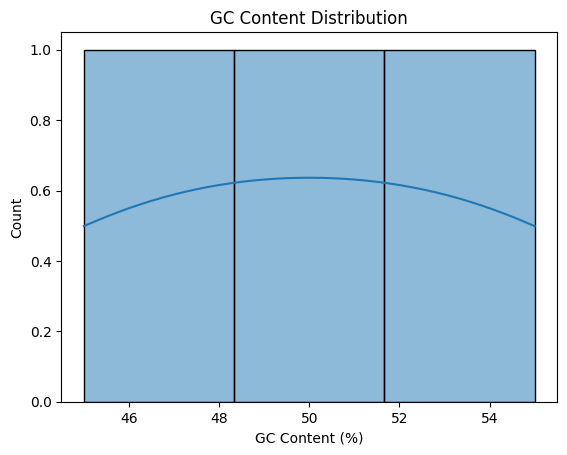
\includegraphics{cnu_introduction_files/figure-pdf/cell-10-output-1.png}

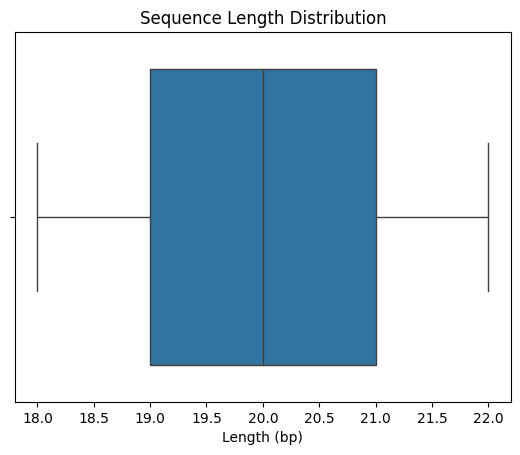
\includegraphics{cnu_introduction_files/figure-pdf/cell-10-output-2.png}

\bookmarksetup{startatroot}

\chapter{Python Basics}\label{python-basics}

\section{구글 드라이브
연결}\label{uxad6cuxae00-uxb4dcuxb77cuxc774uxbe0c-uxc5f0uxacb0}

\begin{itemize}
\tightlist
\item
  세션이 다시 시작 될 때에도 실행 필요
\end{itemize}

\begin{Shaded}
\begin{Highlighting}[]
\OperatorTok{!}\NormalTok{pwd}
\end{Highlighting}
\end{Shaded}

\begin{Shaded}
\begin{Highlighting}[]
\ImportTok{from}\NormalTok{ google.colab }\ImportTok{import}\NormalTok{ drive}
\ImportTok{import}\NormalTok{ os}

\NormalTok{drive.mount(}\StringTok{\textquotesingle{}/content/drive\textquotesingle{}}\NormalTok{)}
\NormalTok{os.chdir(}\StringTok{\textquotesingle{}drive/MyDrive/2024{-}cnu{-}lecture\textquotesingle{}}\NormalTok{)}
\end{Highlighting}
\end{Shaded}

\begin{Shaded}
\begin{Highlighting}[]
\OperatorTok{!}\NormalTok{pwd}
\end{Highlighting}
\end{Shaded}

\section{{[}User{]}}\label{user-2}

{ Okay, I'll learn ``1. Basic Python Programming''. Can you teach me
with a brief explanation and examples }

\section{{[}ChatGPT{]}}\label{chatgpt-2}

Absolutely! Let's start with the basics of Python programming. I'll
cover fundamental concepts with brief explanations and examples to get
you started.

\section{Python Syntax and Semantics}\label{python-syntax-and-semantics}

\subsection{Hello World}\label{hello-world}

The simplest Python program:

\begin{Shaded}
\begin{Highlighting}[]
\BuiltInTok{print}\NormalTok{(}\StringTok{"Hello, World!"}\NormalTok{)}
\end{Highlighting}
\end{Shaded}

\section{Variables and Data Types}\label{variables-and-data-types}

Python supports various data types including integers, floats, strings,
and booleans.

\begin{Shaded}
\begin{Highlighting}[]
\CommentTok{\# Integer}
\NormalTok{a }\OperatorTok{=} \DecValTok{10}

\CommentTok{\# Float}
\NormalTok{b }\OperatorTok{=} \FloatTok{3.14}

\CommentTok{\# String}
\NormalTok{c }\OperatorTok{=} \StringTok{"Hello, Python"}

\CommentTok{\# Boolean}
\NormalTok{d }\OperatorTok{=} \VariableTok{True}

\BuiltInTok{print}\NormalTok{(a, b, c, d)}
\end{Highlighting}
\end{Shaded}

\begin{verbatim}
10 3.14 Hello, Python True
\end{verbatim}

\section{Control Structures}\label{control-structures}

\subsection{If-Else Statements}\label{if-else-statements}

Used for decision making.

\begin{Shaded}
\begin{Highlighting}[]
\NormalTok{x }\OperatorTok{=} \DecValTok{10}
\ControlFlowTok{if}\NormalTok{ x }\OperatorTok{\textgreater{}} \DecValTok{5}\NormalTok{:}
    \BuiltInTok{print}\NormalTok{(}\StringTok{"x is greater than 5"}\NormalTok{)}
\ControlFlowTok{else}\NormalTok{:}
    \BuiltInTok{print}\NormalTok{(}\StringTok{"x is 5 or less"}\NormalTok{)}
\end{Highlighting}
\end{Shaded}

\begin{verbatim}
x is greater than 5
\end{verbatim}

\subsection{Loops}\label{loops}

For repeating tasks.

\begin{Shaded}
\begin{Highlighting}[]
\ControlFlowTok{for}\NormalTok{ i }\KeywordTok{in} \BuiltInTok{range}\NormalTok{(}\DecValTok{5}\NormalTok{):}
    \BuiltInTok{print}\NormalTok{(i)}
\end{Highlighting}
\end{Shaded}

\begin{verbatim}
0
1
2
3
4
\end{verbatim}

\begin{Shaded}
\begin{Highlighting}[]
\NormalTok{i }\OperatorTok{=} \DecValTok{0}
\ControlFlowTok{while}\NormalTok{ i }\OperatorTok{\textless{}} \DecValTok{5}\NormalTok{:}
    \BuiltInTok{print}\NormalTok{(i)}
\NormalTok{    i }\OperatorTok{+=} \DecValTok{1}
\end{Highlighting}
\end{Shaded}

\begin{verbatim}
0
1
2
3
4
\end{verbatim}

\subsection{Functions}\label{functions}

\subsubsection{Defining Functions}\label{defining-functions}

Reusable blocks of code.

\begin{Shaded}
\begin{Highlighting}[]
\KeywordTok{def}\NormalTok{ greet(name):}
    \ControlFlowTok{return} \SpecialStringTok{f"Hello, }\SpecialCharTok{\{}\NormalTok{name}\SpecialCharTok{\}}\SpecialStringTok{"}

\BuiltInTok{print}\NormalTok{(greet(}\StringTok{"Alice"}\NormalTok{))}
\end{Highlighting}
\end{Shaded}

\begin{verbatim}
Hello, Alice
\end{verbatim}

\begin{Shaded}
\begin{Highlighting}[]
\NormalTok{names }\OperatorTok{=}\NormalTok{ [}\StringTok{"Alice"}\NormalTok{, }\StringTok{"Bob"}\NormalTok{, }\StringTok{"Charlie"}\NormalTok{]}

\ControlFlowTok{for}\NormalTok{ name }\KeywordTok{in}\NormalTok{ names:}
  \BuiltInTok{print}\NormalTok{ (}\StringTok{"My name is "}\NormalTok{, name)}
\end{Highlighting}
\end{Shaded}

\begin{verbatim}
My name is  Alice
My name is  Bob
My name is  Charlie
\end{verbatim}

\begin{itemize}
\tightlist
\item
  리스트 값 평균 리턴하는 함수
\end{itemize}

\begin{Shaded}
\begin{Highlighting}[]
\KeywordTok{def}\NormalTok{ average(}\BuiltInTok{input}\NormalTok{):}
    \ControlFlowTok{if} \BuiltInTok{len}\NormalTok{(}\BuiltInTok{input}\NormalTok{) }\OperatorTok{==} \DecValTok{0}\NormalTok{:}
        \ControlFlowTok{return} \VariableTok{None}
    \ControlFlowTok{return} \BuiltInTok{sum}\NormalTok{(}\BuiltInTok{input}\NormalTok{) }\OperatorTok{/} \BuiltInTok{len}\NormalTok{(}\BuiltInTok{input}\NormalTok{)}

\NormalTok{x }\OperatorTok{=}\NormalTok{ [}\DecValTok{1}\NormalTok{,}\DecValTok{2}\NormalTok{,}\DecValTok{3}\NormalTok{,}\DecValTok{4}\NormalTok{,}\DecValTok{5}\NormalTok{,}\DecValTok{6}\NormalTok{,}\DecValTok{7}\NormalTok{,}\DecValTok{8}\NormalTok{,}\DecValTok{9}\NormalTok{,}\DecValTok{10}\NormalTok{]}
\BuiltInTok{print}\NormalTok{(average(x))}
\end{Highlighting}
\end{Shaded}

\begin{verbatim}
5.5
\end{verbatim}

\begin{itemize}
\tightlist
\item
  함수에 대한 개념 이해 중요
\item
  실습과 예제를 통해 이해 필요 (마지막 예제에서 실습)
\end{itemize}

\subsubsection{f-string}\label{f-string}

\begin{itemize}
\tightlist
\item
  f와 \texttt{\{\}} 조합으로 표현할 수 있으며 출력이 고정된 문자열 맨
  앞에 f를 붙여주고, 출력하고 싶은 변수값 등은 중괄호로 표현
\end{itemize}

\begin{Shaded}
\begin{Highlighting}[]
\NormalTok{name }\OperatorTok{=} \StringTok{"Alice"}
\NormalTok{mystr }\OperatorTok{=} \SpecialStringTok{f"My name is }\SpecialCharTok{\{}\NormalTok{name}\SpecialCharTok{\}}\SpecialStringTok{"}

\BuiltInTok{print}\NormalTok{(mystr)}
\end{Highlighting}
\end{Shaded}

\begin{verbatim}
My name is Alice
\end{verbatim}

\begin{Shaded}
\begin{Highlighting}[]
\NormalTok{names }\OperatorTok{=}\NormalTok{ [}\StringTok{"Alice"}\NormalTok{, }\StringTok{"Alisa"}\NormalTok{, }\StringTok{"Alister"}\NormalTok{]}
\NormalTok{mystr }\OperatorTok{=} \SpecialStringTok{f"My name is }\SpecialCharTok{\{}\NormalTok{names}\SpecialCharTok{\}}\SpecialStringTok{"}

\BuiltInTok{print}\NormalTok{(mystr)}
\end{Highlighting}
\end{Shaded}

\begin{verbatim}
My name is ['Alice', 'Alisa', 'Alister']
\end{verbatim}

\begin{Shaded}
\begin{Highlighting}[]
\NormalTok{names }\OperatorTok{=}\NormalTok{ [}\StringTok{"Alice"}\NormalTok{, }\StringTok{"Alisa"}\NormalTok{, }\StringTok{"Alister"}\NormalTok{]}

\ControlFlowTok{for}\NormalTok{ name }\KeywordTok{in}\NormalTok{ names:}
\NormalTok{  mystr }\OperatorTok{=} \SpecialStringTok{f"My name is }\SpecialCharTok{\{}\NormalTok{name}\SpecialCharTok{\}}\SpecialStringTok{"}
  \BuiltInTok{print}\NormalTok{(mystr)}
\end{Highlighting}
\end{Shaded}

\begin{verbatim}
My name is Alice
My name is Alisa
My name is Alister
\end{verbatim}

\section{Lists and Dictionaries}\label{lists-and-dictionaries}

\begin{itemize}
\tightlist
\item
  리스트나 딕셔너리는 파이썬에서 데이터를 저장하는 변수의 자료형임
\item
  여러 종류의 데이터를 효율적으로 활용하기 위한 자료 구조임
\end{itemize}

\subsection{Lists (리스트)}\label{lists-uxb9acuxc2a4uxd2b8}

\begin{itemize}
\tightlist
\item
  Ordered, mutable collections.
\end{itemize}

\begin{Shaded}
\begin{Highlighting}[]
\NormalTok{fruits }\OperatorTok{=}\NormalTok{ [}\StringTok{"apple"}\NormalTok{, }\StringTok{"banana"}\NormalTok{, }\StringTok{"cherry"}\NormalTok{]}
\BuiltInTok{print}\NormalTok{(fruits[}\DecValTok{0}\NormalTok{])  }\CommentTok{\# Accessing elements}
\NormalTok{fruits.append(}\StringTok{"date"}\NormalTok{)  }\CommentTok{\# Adding an element}
\BuiltInTok{print}\NormalTok{(fruits)}
\end{Highlighting}
\end{Shaded}

\begin{verbatim}
apple
['apple', 'banana', 'cherry', 'date']
\end{verbatim}

\begin{itemize}
\tightlist
\item
  인덱싱은 값 자체 (1은 두 번째값)
\item
  슬라이싱은 값 사이 경계선 (1은 첫 번째 값과 두 번째 값 사이)
\item
  아래 그림과 여러 실습 예제를 통한 이해 필요
\end{itemize}

\begin{figure}[H]

{\centering 
\includegraphics{index_files/mediabag/indexing.png}

}

\caption{indexing}

\end{figure}%

\begin{Shaded}
\begin{Highlighting}[]
\NormalTok{geneids }\OperatorTok{=}\NormalTok{ [x }\ControlFlowTok{for}\NormalTok{ x }\KeywordTok{in} \BuiltInTok{range}\NormalTok{(}\DecValTok{10}\NormalTok{)] }\CommentTok{\# 리스트 컴프리헨션}
\BuiltInTok{print}\NormalTok{(geneids)}
\BuiltInTok{print}\NormalTok{(geneids[}\DecValTok{0}\NormalTok{])}
\BuiltInTok{print}\NormalTok{(geneids[}\OperatorTok{{-}}\DecValTok{1}\NormalTok{])}
\BuiltInTok{print}\NormalTok{(geneids[}\DecValTok{2}\NormalTok{:}\DecValTok{5}\NormalTok{])}
\BuiltInTok{print}\NormalTok{(geneids[}\DecValTok{2}\NormalTok{:}\OperatorTok{{-}}\DecValTok{3}\NormalTok{])}
\BuiltInTok{print}\NormalTok{(geneids[:])}
\BuiltInTok{print}\NormalTok{(geneids[:}\OperatorTok{{-}}\DecValTok{1}\NormalTok{])}
\BuiltInTok{print}\NormalTok{(geneids[}\DecValTok{1}\NormalTok{:])}
\end{Highlighting}
\end{Shaded}

\begin{verbatim}
[0, 1, 2, 3, 4, 5, 6, 7, 8, 9]
0
9
[2, 3, 4]
[2, 3, 4, 5, 6]
[0, 1, 2, 3, 4, 5, 6, 7, 8, 9]
[0, 1, 2, 3, 4, 5, 6, 7, 8]
[1, 2, 3, 4, 5, 6, 7, 8, 9]
\end{verbatim}

\begin{itemize}
\tightlist
\item
  리스트 데이터 삽입 삭제
\end{itemize}

\begin{Shaded}
\begin{Highlighting}[]
\NormalTok{geneids }\OperatorTok{=}\NormalTok{ [}\DecValTok{1}\NormalTok{, }\DecValTok{2}\NormalTok{, }\DecValTok{3}\NormalTok{]}
\BuiltInTok{print}\NormalTok{(geneids)}
\NormalTok{geneids.append(}\DecValTok{4}\NormalTok{)}
\BuiltInTok{print}\NormalTok{(geneids)}
\BuiltInTok{print}\NormalTok{(}\StringTok{"length: }\SpecialCharTok{\%d}\StringTok{"} \OperatorTok{\%} \BuiltInTok{len}\NormalTok{(geneids))}
\NormalTok{geneids[}\BuiltInTok{len}\NormalTok{(geneids):] }\OperatorTok{=}\NormalTok{ [}\DecValTok{5}\NormalTok{]}
\BuiltInTok{print}\NormalTok{(geneids)}
\BuiltInTok{print}\NormalTok{(geneids.pop())}
\BuiltInTok{print}\NormalTok{(geneids)}
\end{Highlighting}
\end{Shaded}

\begin{verbatim}
[1, 2, 3]
[1, 2, 3, 4]
length: 4
[1, 2, 3, 4, 5]
5
[1, 2, 3, 4]
\end{verbatim}

\subsection{Tuple (튜플)}\label{tuple-uxd29cuxd50c}

\begin{itemize}
\tightlist
\item
  리스트와 같은 기능이지만 `(', ')'를 사용하고 원소를 변경할 수 없음\\
\item
  리스트보다 빠른 속도, 리스트와 동일한 인덱싱 방법
\end{itemize}

\begin{Shaded}
\begin{Highlighting}[]
\NormalTok{geneids }\OperatorTok{=}\NormalTok{ (}\DecValTok{1}\NormalTok{, }\DecValTok{2}\NormalTok{, }\DecValTok{3}\NormalTok{)}
\BuiltInTok{print}\NormalTok{(geneids[}\DecValTok{0}\NormalTok{:}\DecValTok{2}\NormalTok{])}
\CommentTok{\#geneids[0] = 4 \#\# error}
\end{Highlighting}
\end{Shaded}

\begin{verbatim}
(1, 2)
\end{verbatim}

\begin{itemize}
\tightlist
\item
  반복문에서 리스트 또는 튜플 활용
\end{itemize}

\begin{Shaded}
\begin{Highlighting}[]
\NormalTok{geneids }\OperatorTok{=}\NormalTok{ [}\StringTok{\textquotesingle{}123\textquotesingle{}}\NormalTok{, }\StringTok{\textquotesingle{}456\textquotesingle{}}\NormalTok{, }\StringTok{\textquotesingle{}789\textquotesingle{}}\NormalTok{]}
\ControlFlowTok{for}\NormalTok{ geneid }\KeywordTok{in}\NormalTok{ geneids:}
  \BuiltInTok{print}\NormalTok{(}\SpecialStringTok{f"geneid: }\SpecialCharTok{\{}\NormalTok{geneid}\SpecialCharTok{\}}\SpecialStringTok{"}\NormalTok{)}
\end{Highlighting}
\end{Shaded}

\begin{verbatim}
geneid: 123
geneid: 456
geneid: 789
\end{verbatim}

\subsection{Dictionaries
(딕셔너리)}\label{dictionaries-uxb515uxc154uxb108uxb9ac}

\begin{itemize}
\tightlist
\item
  Key-value pairs, unordered.
\end{itemize}

\begin{Shaded}
\begin{Highlighting}[]
\NormalTok{person }\OperatorTok{=}\NormalTok{ \{}\StringTok{"name"}\NormalTok{: }\StringTok{"Alice"}\NormalTok{, }\StringTok{"age"}\NormalTok{: }\DecValTok{25}\NormalTok{\}}
\BuiltInTok{print}\NormalTok{(person[}\StringTok{"name"}\NormalTok{])}
\NormalTok{person[}\StringTok{"age"}\NormalTok{] }\OperatorTok{=} \DecValTok{26}  \CommentTok{\# Updating value}
\BuiltInTok{print}\NormalTok{(person)}
\end{Highlighting}
\end{Shaded}

\begin{verbatim}
Alice
{'name': 'Alice', 'age': 26}
\end{verbatim}

\begin{itemize}
\tightlist
\item
  키(key)와 값(value)을 쌍으로 저장, `\{'와'\}'를 사용
\end{itemize}

\begin{Shaded}
\begin{Highlighting}[]
\NormalTok{gene\_expr }\OperatorTok{=}\NormalTok{ \{\}}
\NormalTok{gene\_expr[}\StringTok{\textquotesingle{}A\textquotesingle{}}\NormalTok{] }\OperatorTok{=} \FloatTok{0.5}
\BuiltInTok{print}\NormalTok{(gene\_expr)}
\NormalTok{gene\_expr[}\StringTok{\textquotesingle{}B\textquotesingle{}}\NormalTok{] }\OperatorTok{=} \FloatTok{1.2}
\BuiltInTok{print}\NormalTok{(gene\_expr)}
\BuiltInTok{print}\NormalTok{(}\BuiltInTok{len}\NormalTok{(gene\_expr))}
\end{Highlighting}
\end{Shaded}

\begin{verbatim}
{'A': 0.5}
{'A': 0.5, 'B': 1.2}
2
\end{verbatim}

\begin{itemize}
\tightlist
\item
  인덱싱은 `{[}', '{]}' 사용, 키 값으로 인덱싱, 정수값 인덱싱 불가
\end{itemize}

\begin{Shaded}
\begin{Highlighting}[]
\BuiltInTok{print}\NormalTok{(gene\_expr[}\StringTok{\textquotesingle{}A\textquotesingle{}}\NormalTok{])}
\CommentTok{\#\# gene\_expr[0] \# error}
\end{Highlighting}
\end{Shaded}

\begin{verbatim}
0.5
\end{verbatim}

\begin{itemize}
\tightlist
\item
  데이터 추가는 key값 value값으로 수행, 삭제는 del 함수 이용
\end{itemize}

\begin{Shaded}
\begin{Highlighting}[]
\NormalTok{gene\_expr[}\StringTok{\textquotesingle{}C\textquotesingle{}}\NormalTok{] }\OperatorTok{=} \FloatTok{0.3}
\BuiltInTok{print}\NormalTok{(gene\_expr)}
\KeywordTok{del}\NormalTok{ gene\_expr[}\StringTok{\textquotesingle{}C\textquotesingle{}}\NormalTok{]}
\BuiltInTok{print}\NormalTok{(gene\_expr)}
\end{Highlighting}
\end{Shaded}

\begin{verbatim}
{'A': 0.5, 'B': 1.2, 'C': 0.3}
{'A': 0.5, 'B': 1.2}
\end{verbatim}

\begin{itemize}
\tightlist
\item
  key 값과 value 값 구하기
\end{itemize}

\begin{Shaded}
\begin{Highlighting}[]
\NormalTok{gene\_expr\_keys }\OperatorTok{=} \BuiltInTok{list}\NormalTok{(gene\_expr.keys())}
\BuiltInTok{print}\NormalTok{(}\StringTok{"keys:"}\NormalTok{, gene\_expr\_keys)}
\NormalTok{gene\_expr\_values }\OperatorTok{=} \BuiltInTok{list}\NormalTok{(gene\_expr.values())}
\BuiltInTok{print}\NormalTok{(}\StringTok{"values:"}\NormalTok{, gene\_expr\_values)}
\end{Highlighting}
\end{Shaded}

\begin{verbatim}
keys: ['A', 'B']
values: [0.5, 1.2]
\end{verbatim}

\begin{itemize}
\tightlist
\item
  in 활용 키 값 탐색
\end{itemize}

\begin{Shaded}
\begin{Highlighting}[]
\BuiltInTok{print}\NormalTok{(}\StringTok{\textquotesingle{}D\textquotesingle{}} \KeywordTok{in}\NormalTok{ gene\_expr\_keys)}
\BuiltInTok{print}\NormalTok{(}\StringTok{\textquotesingle{}D\textquotesingle{}} \KeywordTok{in}\NormalTok{ gene\_expr)}
\BuiltInTok{print}\NormalTok{(}\StringTok{\textquotesingle{}A\textquotesingle{}} \KeywordTok{in}\NormalTok{ gene\_expr)}
\end{Highlighting}
\end{Shaded}

\begin{verbatim}
False
False
True
\end{verbatim}

\begin{itemize}
\tightlist
\item
  반복문에서 딕셔너리 활용 items()
\end{itemize}

\begin{Shaded}
\begin{Highlighting}[]
\NormalTok{gene\_expr }\OperatorTok{=}\NormalTok{ \{}\StringTok{\textquotesingle{}A\textquotesingle{}}\NormalTok{:}\FloatTok{0.5}\NormalTok{, }\StringTok{\textquotesingle{}B\textquotesingle{}}\NormalTok{:}\FloatTok{1.2}\NormalTok{, }\StringTok{\textquotesingle{}C\textquotesingle{}}\NormalTok{:}\FloatTok{0.3}\NormalTok{, }\StringTok{\textquotesingle{}D\textquotesingle{}}\NormalTok{:}\FloatTok{3.2}\NormalTok{\}}
\ControlFlowTok{for}\NormalTok{ key, val }\KeywordTok{in}\NormalTok{ gene\_expr.items():}
  \BuiltInTok{print}\NormalTok{(}\SpecialStringTok{f"}\SpecialCharTok{\{}\NormalTok{key}\SpecialCharTok{\}}\SpecialStringTok{ expression value is }\SpecialCharTok{\{}\NormalTok{val}\SpecialCharTok{\}}\SpecialStringTok{"}\NormalTok{)}
  \CommentTok{\#print("\%s expression value is \%s" \%(geneid, expval))}
\end{Highlighting}
\end{Shaded}

\begin{verbatim}
A expression value is 0.5
B expression value is 1.2
C expression value is 0.3
D expression value is 3.2
\end{verbatim}

\section{Modules and Packages}\label{modules-and-packages}

\subsection{Importing Modules}\label{importing-modules}

Using standard libraries.

\begin{Shaded}
\begin{Highlighting}[]
\ImportTok{import}\NormalTok{ math}

\BuiltInTok{print}\NormalTok{(math.sqrt(}\DecValTok{16}\NormalTok{))}
\end{Highlighting}
\end{Shaded}

\begin{verbatim}
4.0
\end{verbatim}

\subsection{Importing Specific
Functions}\label{importing-specific-functions}

\begin{Shaded}
\begin{Highlighting}[]
\ImportTok{from}\NormalTok{ math }\ImportTok{import}\NormalTok{ sqrt}

\BuiltInTok{print}\NormalTok{(sqrt(}\DecValTok{25}\NormalTok{))}
\end{Highlighting}
\end{Shaded}

\begin{verbatim}
5.0
\end{verbatim}

\begin{itemize}
\tightlist
\item
  위 average 함수를 mystat.py 라는 이름의 파일로 저장, 모듈로 활용
\end{itemize}

\begin{Shaded}
\begin{Highlighting}[]
\CommentTok{\#import mystat}
\CommentTok{\#x = list(range(10))}
\CommentTok{\#print(mystat.average(x))}
\end{Highlighting}
\end{Shaded}

\begin{itemize}
\tightlist
\item
  모듈 직접 실행시 모듈 내 test 코드 실행 (\textbf{name} ==
  \textbf{main}, True)
\end{itemize}

\begin{Shaded}
\begin{Highlighting}[]
\CommentTok{\#\%run mystat}
\end{Highlighting}
\end{Shaded}

\begin{itemize}
\tightlist
\item
  모듈 임포트
\end{itemize}

\begin{Shaded}
\begin{Highlighting}[]
\ImportTok{import}\NormalTok{ os}
\NormalTok{os.getcwd()}
\end{Highlighting}
\end{Shaded}

\begin{verbatim}
'/home/haseong/lecture/cnu-deeplearning-2024'
\end{verbatim}

\begin{Shaded}
\begin{Highlighting}[]
\ImportTok{from}\NormalTok{ os }\ImportTok{import}\NormalTok{ getcwd}
\NormalTok{getcwd()}
\end{Highlighting}
\end{Shaded}

\begin{verbatim}
'/home/haseong/lecture/cnu-deeplearning-2024'
\end{verbatim}

\section{File I/O}\label{file-io}

\subsection{Writing to a File}\label{writing-to-a-file}

\begin{Shaded}
\begin{Highlighting}[]
\ControlFlowTok{with} \BuiltInTok{open}\NormalTok{(}\StringTok{\textquotesingle{}example.txt\textquotesingle{}}\NormalTok{, }\StringTok{\textquotesingle{}w\textquotesingle{}}\NormalTok{) }\ImportTok{as} \BuiltInTok{file}\NormalTok{:}
    \BuiltInTok{file}\NormalTok{.write(}\StringTok{"Hello, World!"}\NormalTok{)}
\end{Highlighting}
\end{Shaded}

\subsection{Reading from a File}\label{reading-from-a-file}

\begin{Shaded}
\begin{Highlighting}[]

\ControlFlowTok{with} \BuiltInTok{open}\NormalTok{(}\StringTok{\textquotesingle{}example.txt\textquotesingle{}}\NormalTok{, }\StringTok{\textquotesingle{}r\textquotesingle{}}\NormalTok{) }\ImportTok{as} \BuiltInTok{file}\NormalTok{:}
\NormalTok{    content }\OperatorTok{=} \BuiltInTok{file}\NormalTok{.read()}
    \BuiltInTok{print}\NormalTok{(content)}
\end{Highlighting}
\end{Shaded}

\subsection{Example: Basic DNA Sequence
Manipulation}\label{example-basic-dna-sequence-manipulation}

Let's put some of these concepts together with a simple example that
manipulates a DNA sequence.

\begin{Shaded}
\begin{Highlighting}[]
\CommentTok{\# Define a DNA sequence}
\NormalTok{dna\_seq }\OperatorTok{=} \StringTok{"ATGCGTACGTAGCTAGCTAG"}

\CommentTok{\# Function to compute GC content}
\KeywordTok{def}\NormalTok{ gc\_content(seq):}
\NormalTok{    gc\_count }\OperatorTok{=}\NormalTok{ seq.count(}\StringTok{\textquotesingle{}G\textquotesingle{}}\NormalTok{) }\OperatorTok{+}\NormalTok{ seq.count(}\StringTok{\textquotesingle{}C\textquotesingle{}}\NormalTok{)}
    \ControlFlowTok{return}\NormalTok{ gc\_count }\OperatorTok{/} \BuiltInTok{len}\NormalTok{(seq) }\OperatorTok{*} \DecValTok{100}

\CommentTok{\# Function to get the reverse complement of the sequence}
\KeywordTok{def}\NormalTok{ reverse\_complement(seq):}
\NormalTok{    complement }\OperatorTok{=}\NormalTok{ \{}\StringTok{\textquotesingle{}A\textquotesingle{}}\NormalTok{: }\StringTok{\textquotesingle{}T\textquotesingle{}}\NormalTok{, }\StringTok{\textquotesingle{}T\textquotesingle{}}\NormalTok{: }\StringTok{\textquotesingle{}A\textquotesingle{}}\NormalTok{, }\StringTok{\textquotesingle{}C\textquotesingle{}}\NormalTok{: }\StringTok{\textquotesingle{}G\textquotesingle{}}\NormalTok{, }\StringTok{\textquotesingle{}G\textquotesingle{}}\NormalTok{: }\StringTok{\textquotesingle{}C\textquotesingle{}}\NormalTok{\}}
    \ControlFlowTok{return} \StringTok{\textquotesingle{}\textquotesingle{}}\NormalTok{.join(complement[base] }\ControlFlowTok{for}\NormalTok{ base }\KeywordTok{in} \BuiltInTok{reversed}\NormalTok{(seq))}

\CommentTok{\# Compute GC content}
\NormalTok{gc }\OperatorTok{=}\NormalTok{ gc\_content(dna\_seq)}
\BuiltInTok{print}\NormalTok{(}\SpecialStringTok{f"GC Content: }\SpecialCharTok{\{}\NormalTok{gc}\SpecialCharTok{:.2f\}}\SpecialStringTok{\%"}\NormalTok{)}

\CommentTok{\# Get reverse complement}
\NormalTok{rev\_comp }\OperatorTok{=}\NormalTok{ reverse\_complement(dna\_seq)}
\BuiltInTok{print}\NormalTok{(}\SpecialStringTok{f"Reverse Complement: }\SpecialCharTok{\{}\NormalTok{rev\_comp}\SpecialCharTok{\}}\SpecialStringTok{"}\NormalTok{)}
\end{Highlighting}
\end{Shaded}

\begin{verbatim}
GC Content: 50.00%
Reverse Complement: CTAGCTAGCTACGTACGCAT
\end{verbatim}

\subsection{String join (문자열
붙이기)}\label{string-join-uxbb38uxc790uxc5f4-uxbd99uxc774uxae30}

\begin{Shaded}
\begin{Highlighting}[]
\NormalTok{seq1 }\OperatorTok{=} \StringTok{"ATGC"}
\NormalTok{seq2 }\OperatorTok{=} \StringTok{"TAGC"}
\NormalTok{dna\_seq }\OperatorTok{=}\NormalTok{ seq1 }\OperatorTok{+}\NormalTok{ seq2}

\ControlFlowTok{for}\NormalTok{ base }\KeywordTok{in}\NormalTok{ dna\_seq:}
  \BuiltInTok{print}\NormalTok{(base)}

\BuiltInTok{print}\NormalTok{(}\BuiltInTok{type}\NormalTok{(dna\_seq))}
\end{Highlighting}
\end{Shaded}

\begin{verbatim}
A
T
G
C
T
A
G
C
<class 'str'>
\end{verbatim}

\begin{Shaded}
\begin{Highlighting}[]
\NormalTok{complement }\OperatorTok{=}\NormalTok{ \{}\StringTok{\textquotesingle{}A\textquotesingle{}}\NormalTok{: }\StringTok{\textquotesingle{}T\textquotesingle{}}\NormalTok{, }\StringTok{\textquotesingle{}T\textquotesingle{}}\NormalTok{: }\StringTok{\textquotesingle{}A\textquotesingle{}}\NormalTok{, }\StringTok{\textquotesingle{}C\textquotesingle{}}\NormalTok{: }\StringTok{\textquotesingle{}G\textquotesingle{}}\NormalTok{, }\StringTok{\textquotesingle{}G\textquotesingle{}}\NormalTok{: }\StringTok{\textquotesingle{}C\textquotesingle{}}\NormalTok{\}}

\ControlFlowTok{for}\NormalTok{ base }\KeywordTok{in}\NormalTok{ dna\_seq:}
  \BuiltInTok{print}\NormalTok{(complement [base])}

\NormalTok{dna\_seq\_list }\OperatorTok{=}\NormalTok{ []}
\ControlFlowTok{for}\NormalTok{ base }\KeywordTok{in}\NormalTok{ dna\_seq:}
\NormalTok{  dna\_seq\_list.append(complement[base])}

\BuiltInTok{print}\NormalTok{(dna\_seq\_list)}
\BuiltInTok{print}\NormalTok{(}\BuiltInTok{type}\NormalTok{(dna\_seq\_list))}

\NormalTok{dna\_seq\_comp }\OperatorTok{=} \StringTok{""}\NormalTok{.join (dna\_seq\_list)}
\BuiltInTok{print}\NormalTok{(dna\_seq\_comp)}
\BuiltInTok{print}\NormalTok{(}\BuiltInTok{type}\NormalTok{(dna\_seq\_comp))}
\end{Highlighting}
\end{Shaded}

\begin{verbatim}
T
A
C
G
A
T
C
G
['T', 'A', 'C', 'G', 'A', 'T', 'C', 'G']
<class 'list'>
TACGATCG
<class 'str'>
\end{verbatim}

\begin{Shaded}
\begin{Highlighting}[]
\NormalTok{dna\_seq\_list }\OperatorTok{=}\NormalTok{ [complement[base] }\ControlFlowTok{for}\NormalTok{ base }\KeywordTok{in}\NormalTok{ dna\_seq]}
\BuiltInTok{print}\NormalTok{(dna\_seq\_list)}

\NormalTok{dna\_seq\_comp }\OperatorTok{=} \StringTok{""}\NormalTok{.join(dna\_seq\_list)}
\BuiltInTok{print}\NormalTok{(dna\_seq\_comp)}

\BuiltInTok{print}\NormalTok{(}\StringTok{""}\NormalTok{.join([complement[base] }\ControlFlowTok{for}\NormalTok{ base }\KeywordTok{in}\NormalTok{ dna\_seq]))}
\BuiltInTok{print}\NormalTok{(}\StringTok{""}\NormalTok{.join([complement[base] }\ControlFlowTok{for}\NormalTok{ base }\KeywordTok{in}\NormalTok{ dna\_seq }\ControlFlowTok{if}\NormalTok{ base }\OperatorTok{==} \StringTok{"A"} \KeywordTok{or}\NormalTok{ base }\OperatorTok{==} \StringTok{"T"}\NormalTok{]))}
\end{Highlighting}
\end{Shaded}

\begin{verbatim}
['T', 'A', 'C', 'G', 'A', 'T', 'C', 'G']
TACGATCG
TACGATCG
TAAT
\end{verbatim}

\section{클래스}\label{uxd074uxb798uxc2a4}

\begin{itemize}
\tightlist
\item
  Gene, Strain class 생성 연습
\item
  Gene attribute: name, chromosomal location, length\\
\item
  Strain attribute (변수): name, length of chromosome\\
\item
  Strain method (함수): compute average length of the genes
\end{itemize}

\begin{Shaded}
\begin{Highlighting}[]
\ImportTok{import}\NormalTok{ statistics}
\KeywordTok{class}\NormalTok{ ORF:}
    \KeywordTok{def} \FunctionTok{\_\_init\_\_}\NormalTok{(}\VariableTok{self}\NormalTok{, location, length, seq):}
        \VariableTok{self}\NormalTok{.location }\OperatorTok{=}\NormalTok{ location}
        \VariableTok{self}\NormalTok{.length }\OperatorTok{=}\NormalTok{ length}
        \VariableTok{self}\NormalTok{.sequence }\OperatorTok{=}\NormalTok{ seq}

\KeywordTok{class}\NormalTok{ Strain:}
    \KeywordTok{def} \FunctionTok{\_\_init\_\_}\NormalTok{(}\VariableTok{self}\NormalTok{, name, chrlength):}
        \VariableTok{self}\NormalTok{.name }\OperatorTok{=}\NormalTok{ name}
        \VariableTok{self}\NormalTok{.chr\_length }\OperatorTok{=}\NormalTok{ chrlength}
        \VariableTok{self}\NormalTok{.orfs }\OperatorTok{=}\NormalTok{ []}
    \KeywordTok{def}\NormalTok{ add\_orf(}\VariableTok{self}\NormalTok{, location, length, seq):}
        \VariableTok{self}\NormalTok{.orfs.append(ORF(location, length, seq))}
    \KeywordTok{def}\NormalTok{ orf\_length\_average(}\VariableTok{self}\NormalTok{):}
        \ControlFlowTok{return}\NormalTok{ statistics.mean([s.length }\ControlFlowTok{for}\NormalTok{ s }\KeywordTok{in} \VariableTok{self}\NormalTok{.orfs])}
\end{Highlighting}
\end{Shaded}

\begin{Shaded}
\begin{Highlighting}[]
\NormalTok{ecoli }\OperatorTok{=}\NormalTok{ Strain(}\StringTok{"ecoli"}\NormalTok{, }\DecValTok{5000000}\NormalTok{)}
\NormalTok{ecoli.add\_orf(}\DecValTok{1}\NormalTok{, }\DecValTok{1000}\NormalTok{, }\StringTok{"ATG"}\NormalTok{)}
\NormalTok{ecoli.add\_orf(}\DecValTok{1001}\NormalTok{, }\DecValTok{2000}\NormalTok{, }\StringTok{"CCT"}\NormalTok{)}
\NormalTok{ecoli.add\_orf(}\DecValTok{2001}\NormalTok{, }\DecValTok{3000}\NormalTok{, }\StringTok{"ATC"}\NormalTok{)}
\end{Highlighting}
\end{Shaded}

\begin{Shaded}
\begin{Highlighting}[]
\BuiltInTok{print}\NormalTok{([g.location }\ControlFlowTok{for}\NormalTok{ g }\KeywordTok{in}\NormalTok{ ecoli.orfs])}
\BuiltInTok{print}\NormalTok{([g.sequence }\ControlFlowTok{for}\NormalTok{ g }\KeywordTok{in}\NormalTok{ ecoli.orfs])}
\NormalTok{ecoli.orf\_length\_average()}
\end{Highlighting}
\end{Shaded}

\begin{verbatim}
[1, 1001, 2001]
['ATG', 'CCT', 'ATC']
\end{verbatim}

\begin{verbatim}
2000
\end{verbatim}

\begin{itemize}
\tightlist
\item
  상속
\end{itemize}

\begin{Shaded}
\begin{Highlighting}[]
\KeywordTok{class}\NormalTok{ Gene(ORF):}
    \KeywordTok{def}\NormalTok{ add\_protein(}\VariableTok{self}\NormalTok{, prot\_name, prot\_seq):}
        \VariableTok{self}\NormalTok{.prot\_name }\OperatorTok{=}\NormalTok{ prot\_name}
        \VariableTok{self}\NormalTok{.prot\_sequence }\OperatorTok{=}\NormalTok{ prot\_seq}
        
\end{Highlighting}
\end{Shaded}

\begin{Shaded}
\begin{Highlighting}[]
\NormalTok{gene1 }\OperatorTok{=}\NormalTok{ Gene(}\DecValTok{1}\NormalTok{, }\DecValTok{1000}\NormalTok{, }\StringTok{"ATG"}\NormalTok{)}
\BuiltInTok{print}\NormalTok{(gene1.location)}
\NormalTok{gene1.add\_protein(}\StringTok{"myprotein"}\NormalTok{, }\StringTok{"M"}\NormalTok{)}
\BuiltInTok{print}\NormalTok{(gene1.prot\_name)}
\end{Highlighting}
\end{Shaded}

\begin{verbatim}
1
myprotein
\end{verbatim}

\section{Example: Synonymous Mutant Library
Generation}\label{example-synonymous-mutant-library-generation}

\subsection{{[}User{]}}\label{user-3}

I want to generate mutant library of a protein. I have a nucleotide
genbank file for the target protein. I wan to generate all the mutants
by changing synonymous codons for each residue. can you give me the
python code?

\subsection{{[}ChatGPT{]}}\label{chatgpt-3}

Certainly! To generate a mutant library by changing synonymous codons
for each residue of a protein, we'll need to:

\begin{enumerate}
\def\labelenumi{\arabic{enumi}.}
\tightlist
\item
  Read the nucleotide sequence from a GenBank file.
\item
  Translate the nucleotide sequence to a protein sequence.
\item
  Identify synonymous codons for each amino acid.
\item
  Generate all possible synonymous mutants for the target protein.
\end{enumerate}

Here is the Python code that accomplishes these tasks:

\begin{itemize}
\tightlist
\item
  이 예제는 위 프롬프트로 ChatGPT가 만든 코드입니다
\end{itemize}

\subsubsection{Install Necessary
Libraries}\label{install-necessary-libraries}

Make sure you have Biopython installed:

\begin{Shaded}
\begin{Highlighting}[]
\OperatorTok{!}\NormalTok{pip install biopython}
\end{Highlighting}
\end{Shaded}

\subsubsection{Python Script to Generate Synonymous Mutant
Library}\label{python-script-to-generate-synonymous-mutant-library}

\begin{Shaded}
\begin{Highlighting}[]
\ImportTok{from}\NormalTok{ Bio }\ImportTok{import}\NormalTok{ SeqIO}
\ImportTok{from}\NormalTok{ Bio.Seq }\ImportTok{import}\NormalTok{ Seq}
\ImportTok{from}\NormalTok{ itertools }\ImportTok{import}\NormalTok{ product}

\CommentTok{\# Synonymous codon table}
\NormalTok{synonymous\_codons }\OperatorTok{=}\NormalTok{ \{}
    \StringTok{\textquotesingle{}F\textquotesingle{}}\NormalTok{: [}\StringTok{\textquotesingle{}TTT\textquotesingle{}}\NormalTok{, }\StringTok{\textquotesingle{}TTC\textquotesingle{}}\NormalTok{],}
    \StringTok{\textquotesingle{}L\textquotesingle{}}\NormalTok{: [}\StringTok{\textquotesingle{}TTA\textquotesingle{}}\NormalTok{, }\StringTok{\textquotesingle{}TTG\textquotesingle{}}\NormalTok{, }\StringTok{\textquotesingle{}CTT\textquotesingle{}}\NormalTok{, }\StringTok{\textquotesingle{}CTC\textquotesingle{}}\NormalTok{, }\StringTok{\textquotesingle{}CTA\textquotesingle{}}\NormalTok{, }\StringTok{\textquotesingle{}CTG\textquotesingle{}}\NormalTok{],}
    \StringTok{\textquotesingle{}I\textquotesingle{}}\NormalTok{: [}\StringTok{\textquotesingle{}ATT\textquotesingle{}}\NormalTok{, }\StringTok{\textquotesingle{}ATC\textquotesingle{}}\NormalTok{, }\StringTok{\textquotesingle{}ATA\textquotesingle{}}\NormalTok{],}
    \StringTok{\textquotesingle{}M\textquotesingle{}}\NormalTok{: [}\StringTok{\textquotesingle{}ATG\textquotesingle{}}\NormalTok{],}
    \StringTok{\textquotesingle{}V\textquotesingle{}}\NormalTok{: [}\StringTok{\textquotesingle{}GTT\textquotesingle{}}\NormalTok{, }\StringTok{\textquotesingle{}GTC\textquotesingle{}}\NormalTok{, }\StringTok{\textquotesingle{}GTA\textquotesingle{}}\NormalTok{, }\StringTok{\textquotesingle{}GTG\textquotesingle{}}\NormalTok{],}
    \StringTok{\textquotesingle{}S\textquotesingle{}}\NormalTok{: [}\StringTok{\textquotesingle{}TCT\textquotesingle{}}\NormalTok{, }\StringTok{\textquotesingle{}TCC\textquotesingle{}}\NormalTok{, }\StringTok{\textquotesingle{}TCA\textquotesingle{}}\NormalTok{, }\StringTok{\textquotesingle{}TCG\textquotesingle{}}\NormalTok{, }\StringTok{\textquotesingle{}AGT\textquotesingle{}}\NormalTok{, }\StringTok{\textquotesingle{}AGC\textquotesingle{}}\NormalTok{],}
    \StringTok{\textquotesingle{}P\textquotesingle{}}\NormalTok{: [}\StringTok{\textquotesingle{}CCT\textquotesingle{}}\NormalTok{, }\StringTok{\textquotesingle{}CCC\textquotesingle{}}\NormalTok{, }\StringTok{\textquotesingle{}CCA\textquotesingle{}}\NormalTok{, }\StringTok{\textquotesingle{}CCG\textquotesingle{}}\NormalTok{],}
    \StringTok{\textquotesingle{}T\textquotesingle{}}\NormalTok{: [}\StringTok{\textquotesingle{}ACT\textquotesingle{}}\NormalTok{, }\StringTok{\textquotesingle{}ACC\textquotesingle{}}\NormalTok{, }\StringTok{\textquotesingle{}ACA\textquotesingle{}}\NormalTok{, }\StringTok{\textquotesingle{}ACG\textquotesingle{}}\NormalTok{],}
    \StringTok{\textquotesingle{}A\textquotesingle{}}\NormalTok{: [}\StringTok{\textquotesingle{}GCT\textquotesingle{}}\NormalTok{, }\StringTok{\textquotesingle{}GCC\textquotesingle{}}\NormalTok{, }\StringTok{\textquotesingle{}GCA\textquotesingle{}}\NormalTok{, }\StringTok{\textquotesingle{}GCG\textquotesingle{}}\NormalTok{],}
    \StringTok{\textquotesingle{}Y\textquotesingle{}}\NormalTok{: [}\StringTok{\textquotesingle{}TAT\textquotesingle{}}\NormalTok{, }\StringTok{\textquotesingle{}TAC\textquotesingle{}}\NormalTok{],}
    \StringTok{\textquotesingle{}H\textquotesingle{}}\NormalTok{: [}\StringTok{\textquotesingle{}CAT\textquotesingle{}}\NormalTok{, }\StringTok{\textquotesingle{}CAC\textquotesingle{}}\NormalTok{],}
    \StringTok{\textquotesingle{}Q\textquotesingle{}}\NormalTok{: [}\StringTok{\textquotesingle{}CAA\textquotesingle{}}\NormalTok{, }\StringTok{\textquotesingle{}CAG\textquotesingle{}}\NormalTok{],}
    \StringTok{\textquotesingle{}N\textquotesingle{}}\NormalTok{: [}\StringTok{\textquotesingle{}AAT\textquotesingle{}}\NormalTok{, }\StringTok{\textquotesingle{}AAC\textquotesingle{}}\NormalTok{],}
    \StringTok{\textquotesingle{}K\textquotesingle{}}\NormalTok{: [}\StringTok{\textquotesingle{}AAA\textquotesingle{}}\NormalTok{, }\StringTok{\textquotesingle{}AAG\textquotesingle{}}\NormalTok{],}
    \StringTok{\textquotesingle{}D\textquotesingle{}}\NormalTok{: [}\StringTok{\textquotesingle{}GAT\textquotesingle{}}\NormalTok{, }\StringTok{\textquotesingle{}GAC\textquotesingle{}}\NormalTok{],}
    \StringTok{\textquotesingle{}E\textquotesingle{}}\NormalTok{: [}\StringTok{\textquotesingle{}GAA\textquotesingle{}}\NormalTok{, }\StringTok{\textquotesingle{}GAG\textquotesingle{}}\NormalTok{],}
    \StringTok{\textquotesingle{}C\textquotesingle{}}\NormalTok{: [}\StringTok{\textquotesingle{}TGT\textquotesingle{}}\NormalTok{, }\StringTok{\textquotesingle{}TGC\textquotesingle{}}\NormalTok{],}
    \StringTok{\textquotesingle{}W\textquotesingle{}}\NormalTok{: [}\StringTok{\textquotesingle{}TGG\textquotesingle{}}\NormalTok{],}
    \StringTok{\textquotesingle{}R\textquotesingle{}}\NormalTok{: [}\StringTok{\textquotesingle{}CGT\textquotesingle{}}\NormalTok{, }\StringTok{\textquotesingle{}CGC\textquotesingle{}}\NormalTok{, }\StringTok{\textquotesingle{}CGA\textquotesingle{}}\NormalTok{, }\StringTok{\textquotesingle{}CGG\textquotesingle{}}\NormalTok{, }\StringTok{\textquotesingle{}AGA\textquotesingle{}}\NormalTok{, }\StringTok{\textquotesingle{}AGG\textquotesingle{}}\NormalTok{],}
    \StringTok{\textquotesingle{}G\textquotesingle{}}\NormalTok{: [}\StringTok{\textquotesingle{}GGT\textquotesingle{}}\NormalTok{, }\StringTok{\textquotesingle{}GGC\textquotesingle{}}\NormalTok{, }\StringTok{\textquotesingle{}GGA\textquotesingle{}}\NormalTok{, }\StringTok{\textquotesingle{}GGG\textquotesingle{}}\NormalTok{],}
    \StringTok{\textquotesingle{}*\textquotesingle{}}\NormalTok{: [}\StringTok{\textquotesingle{}TAA\textquotesingle{}}\NormalTok{, }\StringTok{\textquotesingle{}TAG\textquotesingle{}}\NormalTok{, }\StringTok{\textquotesingle{}TGA\textquotesingle{}}\NormalTok{]}
\NormalTok{\}}

\CommentTok{\# Function to read the GenBank file and extract the coding sequence}
\KeywordTok{def}\NormalTok{ read\_cds\_from\_genbank(file\_path):}
\NormalTok{    record }\OperatorTok{=}\NormalTok{ SeqIO.read(file\_path, }\StringTok{"genbank"}\NormalTok{)}
    \ControlFlowTok{for}\NormalTok{ feature }\KeywordTok{in}\NormalTok{ record.features:}
        \ControlFlowTok{if}\NormalTok{ feature.}\BuiltInTok{type} \OperatorTok{==} \StringTok{"CDS"}\NormalTok{:}
            \ControlFlowTok{return}\NormalTok{ feature.location.extract(record).seq}
    \ControlFlowTok{raise} \PreprocessorTok{ValueError}\NormalTok{(}\StringTok{"No CDS found in the GenBank file."}\NormalTok{)}

\CommentTok{\# Function to generate synonymous mutants}
\KeywordTok{def}\NormalTok{ generate\_synonymous\_mutants(cds\_seq):}
\NormalTok{    protein\_seq }\OperatorTok{=}\NormalTok{ cds\_seq.translate()}
\NormalTok{    codon\_options }\OperatorTok{=}\NormalTok{ []}

    \ControlFlowTok{for}\NormalTok{ aa }\KeywordTok{in}\NormalTok{ protein\_seq[:}\DecValTok{5}\NormalTok{]:}
\NormalTok{        codons }\OperatorTok{=}\NormalTok{ synonymous\_codons.get(aa, [])}
        \ControlFlowTok{if} \KeywordTok{not}\NormalTok{ codons:}
            \ControlFlowTok{raise} \PreprocessorTok{ValueError}\NormalTok{(}\SpecialStringTok{f"Unknown amino acid }\SpecialCharTok{\{}\NormalTok{aa}\SpecialCharTok{\}}\SpecialStringTok{ encountered."}\NormalTok{)}
\NormalTok{        codon\_options.append(codons)}

    \CommentTok{\# Generate all combinations of synonymous codons}
\NormalTok{    all\_mutants }\OperatorTok{=} \BuiltInTok{list}\NormalTok{(product(}\OperatorTok{*}\NormalTok{codon\_options))}
    \ControlFlowTok{return}\NormalTok{ [}\StringTok{\textquotesingle{}\textquotesingle{}}\NormalTok{.join(mutant) }\ControlFlowTok{for}\NormalTok{ mutant }\KeywordTok{in}\NormalTok{ all\_mutants]}

\CommentTok{\# Main function}
\KeywordTok{def}\NormalTok{ main(genbank\_file, output\_file):}
\NormalTok{    cds\_seq }\OperatorTok{=}\NormalTok{ read\_cds\_from\_genbank(genbank\_file)}
\NormalTok{    mutants }\OperatorTok{=}\NormalTok{ generate\_synonymous\_mutants(cds\_seq)}

    \CommentTok{\# Write the mutants to a FASTA file}
    \ControlFlowTok{with} \BuiltInTok{open}\NormalTok{(output\_file, }\StringTok{\textquotesingle{}w\textquotesingle{}}\NormalTok{) }\ImportTok{as}\NormalTok{ f:}
        \ControlFlowTok{for}\NormalTok{ i, mutant }\KeywordTok{in} \BuiltInTok{enumerate}\NormalTok{(mutants):}
\NormalTok{            f.write(}\SpecialStringTok{f"\textgreater{}Mutant\_}\SpecialCharTok{\{}\NormalTok{i}\OperatorTok{+}\DecValTok{1}\SpecialCharTok{\}}\CharTok{\textbackslash{}n}\SpecialCharTok{\{}\NormalTok{mutant}\SpecialCharTok{\}}\CharTok{\textbackslash{}n}\SpecialStringTok{"}\NormalTok{)}

\CommentTok{\# Example usage}
\NormalTok{genbank\_file }\OperatorTok{=} \StringTok{\textquotesingle{}data/egfp.gb\textquotesingle{}}  \CommentTok{\# Replace with your GenBank file path}
\NormalTok{output\_file }\OperatorTok{=} \StringTok{\textquotesingle{}mutant\_library.fasta\textquotesingle{}}
\NormalTok{main(genbank\_file, output\_file)}
\end{Highlighting}
\end{Shaded}

\begin{itemize}
\tightlist
\item
  위 코드를 두 개의 파일로 나누어 (함수모음 파일, 실행 파일) 모듈 실습
  가능
\end{itemize}

\bookmarksetup{startatroot}

\chapter{Data handling}\label{data-handling}

\textbf{구글 드라이브 연결}

\begin{Shaded}
\begin{Highlighting}[]
\OperatorTok{!}\NormalTok{pwd}
\end{Highlighting}
\end{Shaded}

\begin{verbatim}
/home/haseong/lecture/cnu-deeplearning-2024
\end{verbatim}

\begin{Shaded}
\begin{Highlighting}[]
\ImportTok{from}\NormalTok{ google.colab }\ImportTok{import}\NormalTok{ drive}
\ImportTok{import}\NormalTok{ os}

\NormalTok{drive.mount(}\StringTok{\textquotesingle{}/content/drive\textquotesingle{}}\NormalTok{)}
\NormalTok{os.chdir(}\StringTok{\textquotesingle{}drive/MyDrive/2024{-}cnu{-}lecture\textquotesingle{}}\NormalTok{)}
\end{Highlighting}
\end{Shaded}

\begin{Shaded}
\begin{Highlighting}[]
\OperatorTok{!}\NormalTok{pwd}
\end{Highlighting}
\end{Shaded}

\subsection{{[}User{]}}\label{user-4}

{ I want to learn ``2. Data Handling and Analysis''. can you explain me
a brief explanation and examples? }

\subsection{{[}ChatGPT{]}}\label{chatgpt-4}

Sure! Data handling and analysis are essential skills in Python,
especially for tasks like manipulating datasets, performing statistical
analyses, and creating visualizations. We'll focus on the key libraries
used for these purposes: NumPy, Pandas, and Matplotlib/Seaborn.

\subsection{1. NumPy}\label{numpy}

NumPy is a powerful library for numerical operations and handling
arrays.

\subsubsection{Basics of NumPy}\label{basics-of-numpy}

\textbf{Installation:}

\begin{Shaded}
\begin{Highlighting}[]
\ExtensionTok{!pip}\NormalTok{ install numpy}
\end{Highlighting}
\end{Shaded}

\begin{Shaded}
\begin{Highlighting}[]
\ImportTok{import}\NormalTok{ numpy }\ImportTok{as}\NormalTok{ np}


\CommentTok{\# Creating a 1D array}
\NormalTok{arr1 }\OperatorTok{=}\NormalTok{ np.array([}\DecValTok{1}\NormalTok{, }\DecValTok{2}\NormalTok{, }\DecValTok{3}\NormalTok{, }\DecValTok{4}\NormalTok{, }\DecValTok{5}\NormalTok{])}

\CommentTok{\# Creating a 2D array}
\NormalTok{arr2 }\OperatorTok{=}\NormalTok{ np.array([[}\DecValTok{1}\NormalTok{, }\DecValTok{2}\NormalTok{, }\DecValTok{3}\NormalTok{], [}\DecValTok{4}\NormalTok{, }\DecValTok{5}\NormalTok{, }\DecValTok{6}\NormalTok{]])}

\BuiltInTok{print}\NormalTok{(arr1)}
\BuiltInTok{print}\NormalTok{(arr2)}


\CommentTok{\# Element{-}wise operations}
\NormalTok{arr3 }\OperatorTok{=}\NormalTok{ arr1 }\OperatorTok{*} \DecValTok{2}
\BuiltInTok{print}\NormalTok{(arr3)}

\CommentTok{\# Mathematical functions}
\BuiltInTok{print}\NormalTok{(np.sqrt(arr1))}
\end{Highlighting}
\end{Shaded}

\begin{verbatim}
[1 2 3 4 5]
[[1 2 3]
 [4 5 6]]
[ 2  4  6  8 10]
[1.         1.41421356 1.73205081 2.         2.23606798]
\end{verbatim}

\subsubsection{Numpy 자료구조
ndarray}\label{numpy-uxc790uxb8ccuxad6cuxc870-ndarray}

\begin{itemize}
\tightlist
\item
  행렬이나 다차원 배열 처리용 파이썬 라이브러리
\item
  같은 타입의 데이터만 허용
\item
  리스트에 비해 20배 이상 빠른 속도
\end{itemize}

\begin{figure}[H]

{\centering 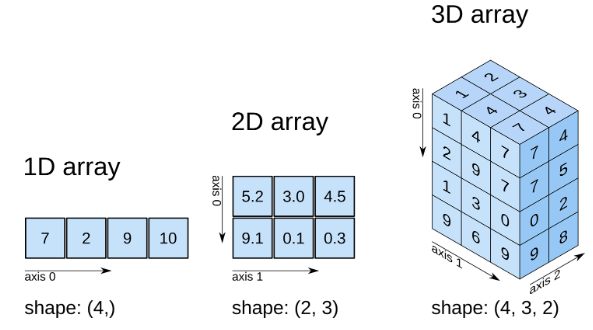
\includegraphics{index_files/mediabag/numpy.png}

}

\caption{from
https://www.oreilly.com/library/view/elegant-scipy/9781491922927/ch01.html}

\end{figure}%

\begin{itemize}
\tightlist
\item
  numpy 객체 만들기
\end{itemize}

\begin{Shaded}
\begin{Highlighting}[]
\ImportTok{import}\NormalTok{ numpy }\ImportTok{as}\NormalTok{ np}

\NormalTok{arr }\OperatorTok{=}\NormalTok{ [}\DecValTok{1}\NormalTok{, }\DecValTok{2}\NormalTok{, }\DecValTok{3}\NormalTok{]}
\BuiltInTok{print}\NormalTok{(arr)}
\BuiltInTok{print}\NormalTok{(}\BuiltInTok{type}\NormalTok{(arr))}

\NormalTok{a }\OperatorTok{=}\NormalTok{ np.array([}\DecValTok{1}\NormalTok{,}\DecValTok{2}\NormalTok{,}\DecValTok{3}\NormalTok{])}
\BuiltInTok{print}\NormalTok{(a)}
\BuiltInTok{print}\NormalTok{(a.dtype)}
\BuiltInTok{print}\NormalTok{(a.shape)}
\BuiltInTok{print}\NormalTok{(}\BuiltInTok{type}\NormalTok{(a))}
\end{Highlighting}
\end{Shaded}

\begin{verbatim}
[1, 2, 3]
<class 'list'>
[1 2 3]
int64
(3,)
<class 'numpy.ndarray'>
\end{verbatim}

\begin{Shaded}
\begin{Highlighting}[]
\NormalTok{arr2 }\OperatorTok{=}\NormalTok{ np.array([[}\DecValTok{1}\NormalTok{,}\DecValTok{2}\NormalTok{,}\DecValTok{3}\NormalTok{], [}\DecValTok{4}\NormalTok{,}\DecValTok{5}\NormalTok{,}\DecValTok{6}\NormalTok{]])}
\BuiltInTok{print}\NormalTok{(arr2)}
\BuiltInTok{print}\NormalTok{(}\BuiltInTok{type}\NormalTok{(arr2))}
\BuiltInTok{print}\NormalTok{(arr2.shape)}
\BuiltInTok{print}\NormalTok{(arr2.dtype)}
\end{Highlighting}
\end{Shaded}

\begin{verbatim}
[[1 2 3]
 [4 5 6]]
<class 'numpy.ndarray'>
(2, 3)
int64
\end{verbatim}

\begin{itemize}
\tightlist
\item
  numpy 자료형

  \begin{itemize}
  \tightlist
  \item
    부호가 있는 정수 int(8, 16, 32, 64)
  \item
    부호가 없는 정수 uint(8 ,16, 32, 54)
  \item
    실수 float(16, 32, 64, 128)
  \item
    복소수 complex(64, 128, 256)
  \item
    불리언 bool
  \item
    문자열 string\_
  \item
    파이썬 오프젝트 object
  \item
    유니코드 unicode\_
  \end{itemize}
\item
  np.zeros(), np.ones(), np.arange()
\item
  행렬 연산 지원
\end{itemize}

\begin{Shaded}
\begin{Highlighting}[]
\NormalTok{a }\OperatorTok{=}\NormalTok{ np.arange(}\DecValTok{1}\NormalTok{, }\DecValTok{10}\NormalTok{).reshape(}\DecValTok{3}\NormalTok{,}\DecValTok{3}\NormalTok{) }\CommentTok{\# [1, 10)}
\BuiltInTok{print}\NormalTok{(a)}
\NormalTok{a }\OperatorTok{=}\NormalTok{ np.ones((}\DecValTok{3}\NormalTok{,}\DecValTok{4}\NormalTok{), dtype}\OperatorTok{=}\NormalTok{np.int16)}
\NormalTok{b }\OperatorTok{=}\NormalTok{ np.ones((}\DecValTok{3}\NormalTok{,}\DecValTok{4}\NormalTok{), dtype}\OperatorTok{=}\NormalTok{np.int16)}
\BuiltInTok{print}\NormalTok{(a)}
\BuiltInTok{print}\NormalTok{(b)}
\BuiltInTok{print}\NormalTok{(a}\OperatorTok{+}\NormalTok{b)}
\BuiltInTok{print}\NormalTok{(a}\OperatorTok{{-}}\NormalTok{b)}
\end{Highlighting}
\end{Shaded}

\begin{verbatim}
[[1 2 3]
 [4 5 6]
 [7 8 9]]
[[1 1 1 1]
 [1 1 1 1]
 [1 1 1 1]]
[[1 1 1 1]
 [1 1 1 1]
 [1 1 1 1]]
[[2 2 2 2]
 [2 2 2 2]
 [2 2 2 2]]
[[0 0 0 0]
 [0 0 0 0]
 [0 0 0 0]]
\end{verbatim}

\begin{itemize}
\tightlist
\item
  numpy 함수

  \begin{itemize}
  \tightlist
  \item
    np.sqrt()
  \item
    np.log()
  \item
    np.square()
  \item
    np.log()
  \item
    np.ceil()
  \item
    np.floor()
  \item
    np.isnan()
  \item
    np.sum()
  \item
    np.mean()
  \item
    np.std()
  \item
    np.min()
  \end{itemize}
\end{itemize}

\begin{Shaded}
\begin{Highlighting}[]
\BuiltInTok{dir}\NormalTok{(np)}
\end{Highlighting}
\end{Shaded}

\subsection{2. Pandas}\label{pandas}

Pandas is a powerful library for data manipulation and analysis. It
provides data structures like DataFrame, which is similar to tables in
databases or spreadsheets.

\subsubsection{Installation}\label{installation}

\begin{Shaded}
\begin{Highlighting}[]
\ExtensionTok{pip}\NormalTok{ install pandas}
\end{Highlighting}
\end{Shaded}

\begin{itemize}
\tightlist
\item
  Pandas의 Series는 1차원, DataFrame은 2차원 데이터를 다루는 자료구조
\item
  DataFrames are the primary data structure in pandas, representing
  tabular data with rows and columns.
\item
  index, column, values 로 이루어짐
\item
  리스트와 딕셔너리로부터 생성 가능
\item
  숫자형, 문자형, 범주형 등의 다양한 데이터 입력 가능
\end{itemize}

\begin{figure}[H]

{\centering 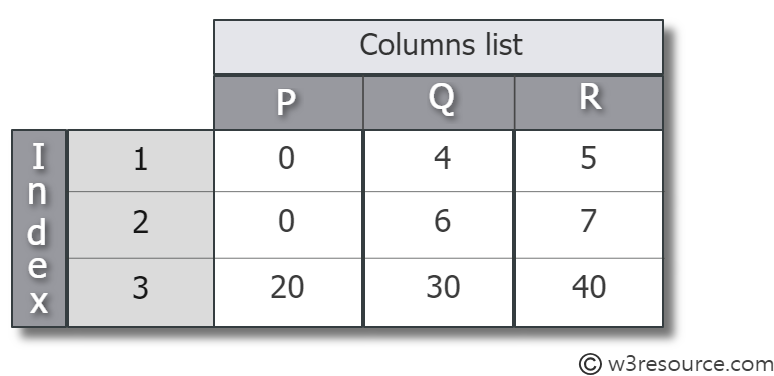
\includegraphics{images/pandas-dataframe-structure.png}

}

\caption{alt text}

\end{figure}%

\begin{Shaded}
\begin{Highlighting}[]
\ImportTok{from}\NormalTok{ pandas }\ImportTok{import}\NormalTok{ Series, DataFrame}
\end{Highlighting}
\end{Shaded}

\begin{Shaded}
\begin{Highlighting}[]
\NormalTok{genes }\OperatorTok{=}\NormalTok{ Series([}\FloatTok{0.1}\NormalTok{, }\FloatTok{0.2}\NormalTok{, }\FloatTok{1.4}\NormalTok{, }\FloatTok{0.6}\NormalTok{, }\FloatTok{1.1}\NormalTok{])}
\BuiltInTok{print}\NormalTok{(genes)}
\end{Highlighting}
\end{Shaded}

\begin{verbatim}
0    0.1
1    0.2
2    1.4
3    0.6
4    1.1
dtype: float64
\end{verbatim}

\begin{Shaded}
\begin{Highlighting}[]
\NormalTok{genes }\OperatorTok{=}\NormalTok{ Series([}\FloatTok{0.1}\NormalTok{, }\FloatTok{0.2}\NormalTok{, }\FloatTok{1.4}\NormalTok{, }\FloatTok{0.6}\NormalTok{, }\FloatTok{1.1}\NormalTok{], index}\OperatorTok{=}\NormalTok{[}\StringTok{\textquotesingle{}A\textquotesingle{}}\NormalTok{, }\StringTok{\textquotesingle{}B\textquotesingle{}}\NormalTok{, }\StringTok{\textquotesingle{}C\textquotesingle{}}\NormalTok{, }\StringTok{\textquotesingle{}D\textquotesingle{}}\NormalTok{, }\StringTok{\textquotesingle{}E\textquotesingle{}}\NormalTok{])}
\BuiltInTok{print}\NormalTok{(genes)}
\end{Highlighting}
\end{Shaded}

\begin{verbatim}
A    0.1
B    0.2
C    1.4
D    0.6
E    1.1
dtype: float64
\end{verbatim}

\subsubsection{Make a DataFrame}\label{make-a-dataframe}

\begin{itemize}
\tightlist
\item
  Create from a list
\end{itemize}

\begin{Shaded}
\begin{Highlighting}[]
\ImportTok{import}\NormalTok{ pandas }\ImportTok{as}\NormalTok{ pd}

\NormalTok{df }\OperatorTok{=}\NormalTok{ pd.DataFrame([[}\DecValTok{0}\NormalTok{, }\DecValTok{4}\NormalTok{, }\DecValTok{5}\NormalTok{], [}\DecValTok{0}\NormalTok{, }\DecValTok{6}\NormalTok{, }\DecValTok{7}\NormalTok{], [}\DecValTok{20}\NormalTok{, }\DecValTok{30}\NormalTok{, }\DecValTok{40}\NormalTok{]],}
\NormalTok{                  index}\OperatorTok{=}\NormalTok{[}\DecValTok{1}\NormalTok{, }\DecValTok{2}\NormalTok{, }\DecValTok{3}\NormalTok{], columns}\OperatorTok{=}\NormalTok{[}\StringTok{\textquotesingle{}P\textquotesingle{}}\NormalTok{, }\StringTok{\textquotesingle{}Q\textquotesingle{}}\NormalTok{, }\StringTok{\textquotesingle{}R\textquotesingle{}}\NormalTok{])}

\BuiltInTok{print}\NormalTok{(df)}
\end{Highlighting}
\end{Shaded}

\begin{verbatim}
    P   Q   R
1   0   4   5
2   0   6   7
3  20  30  40
\end{verbatim}

\begin{itemize}
\tightlist
\item
  Create dataframe from a dictionary
\end{itemize}

\begin{figure}[H]

{\centering 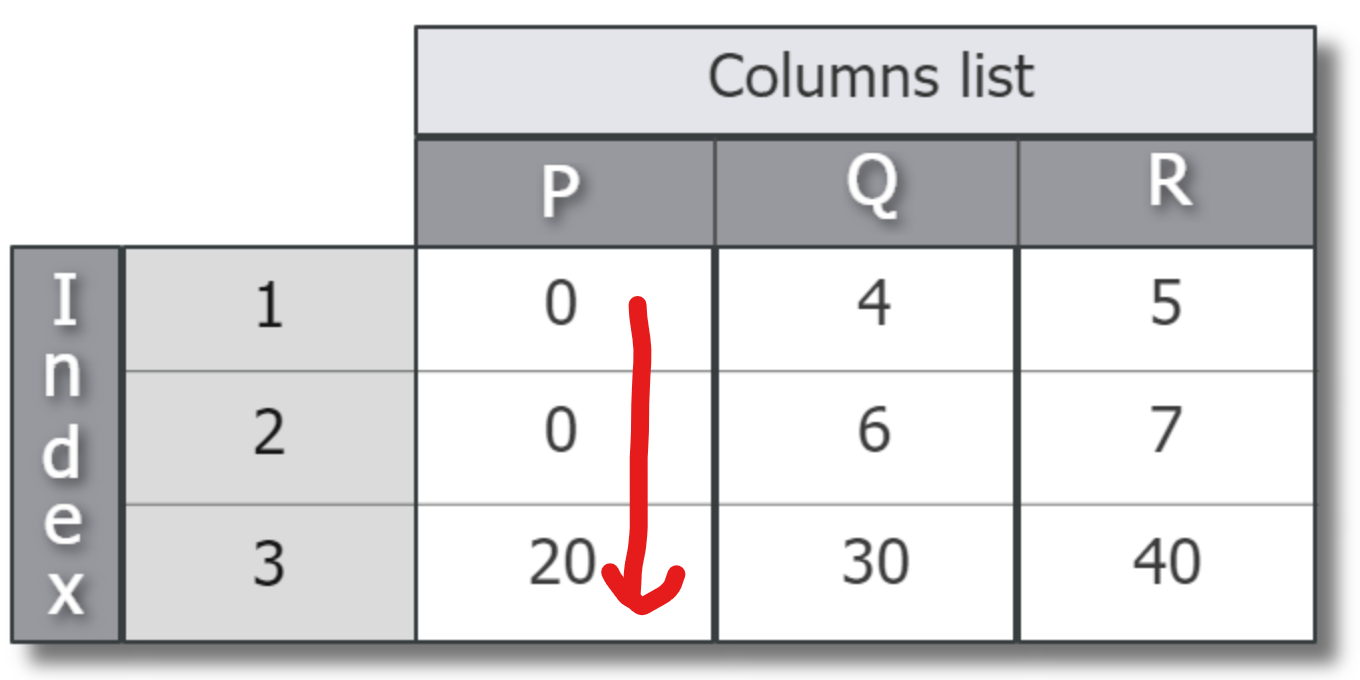
\includegraphics{images/df_from_dic1.png}

}

\caption{alt text}

\end{figure}%

\begin{Shaded}
\begin{Highlighting}[]
\ImportTok{import}\NormalTok{ pandas }\ImportTok{as}\NormalTok{ pd}

\NormalTok{data }\OperatorTok{=}\NormalTok{ \{}
    \StringTok{\textquotesingle{}Name\textquotesingle{}}\NormalTok{: [}\StringTok{\textquotesingle{}Alice\textquotesingle{}}\NormalTok{, }\StringTok{\textquotesingle{}Bob\textquotesingle{}}\NormalTok{, }\StringTok{\textquotesingle{}Charlie\textquotesingle{}}\NormalTok{],}
    \StringTok{\textquotesingle{}Age\textquotesingle{}}\NormalTok{: [}\DecValTok{25}\NormalTok{, }\DecValTok{30}\NormalTok{, }\DecValTok{35}\NormalTok{],}
    \StringTok{\textquotesingle{}Height\textquotesingle{}}\NormalTok{: [}\FloatTok{5.5}\NormalTok{, }\FloatTok{6.0}\NormalTok{, }\FloatTok{5.8}\NormalTok{]}
\NormalTok{\}}

\NormalTok{df }\OperatorTok{=}\NormalTok{ pd.DataFrame(data)}
\BuiltInTok{print}\NormalTok{(df)}
\end{Highlighting}
\end{Shaded}

\begin{verbatim}
      Name  Age  Height
0    Alice   25     5.5
1      Bob   30     6.0
2  Charlie   35     5.8
\end{verbatim}

\begin{itemize}
\tightlist
\item
  Create from a list of dictionary
\end{itemize}

\begin{figure}[H]

{\centering 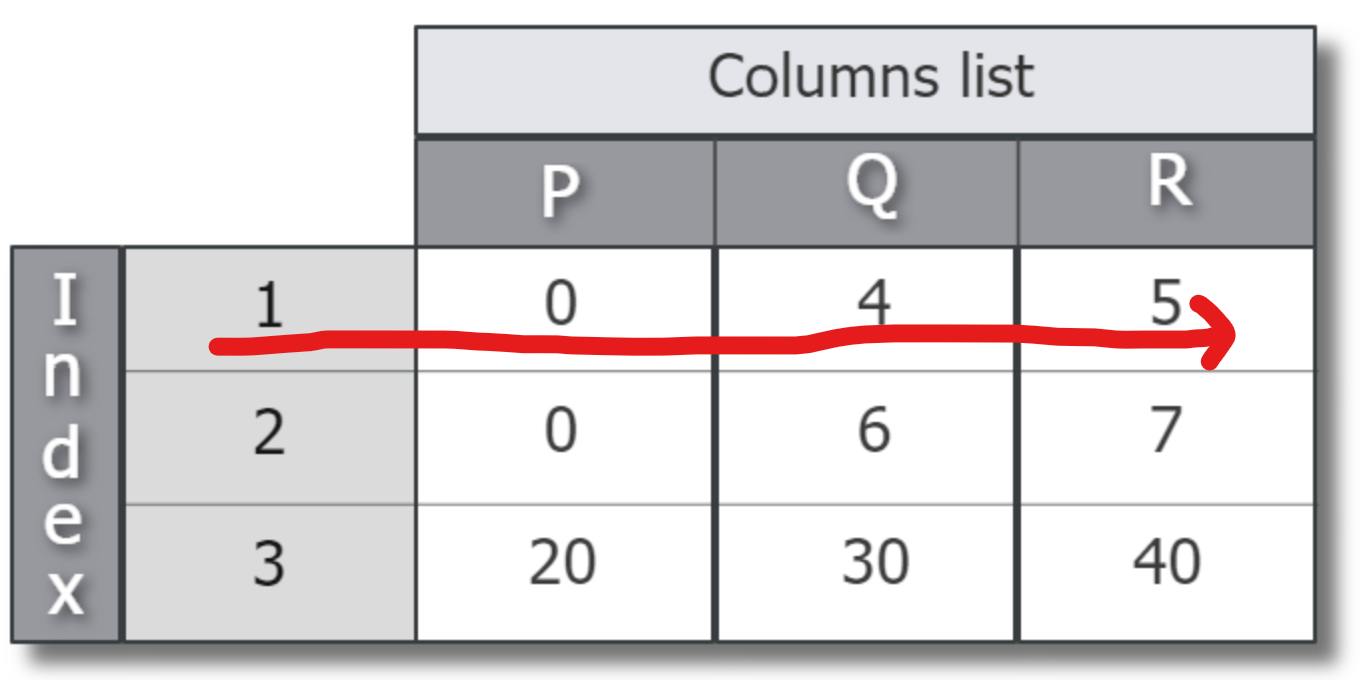
\includegraphics{images/df_from_dic2.png}

}

\caption{alt text}

\end{figure}%

\begin{Shaded}
\begin{Highlighting}[]
\NormalTok{data }\OperatorTok{=}\NormalTok{ [}
\NormalTok{    \{}\StringTok{\textquotesingle{}Name\textquotesingle{}}\NormalTok{: }\StringTok{\textquotesingle{}Alice\textquotesingle{}}\NormalTok{, }\StringTok{\textquotesingle{}Age\textquotesingle{}}\NormalTok{: }\DecValTok{25}\NormalTok{, }\StringTok{\textquotesingle{}Height\textquotesingle{}}\NormalTok{: }\FloatTok{5.5}\NormalTok{\},}
\NormalTok{    \{}\StringTok{\textquotesingle{}Name\textquotesingle{}}\NormalTok{: }\StringTok{\textquotesingle{}Bob\textquotesingle{}}\NormalTok{, }\StringTok{\textquotesingle{}Age\textquotesingle{}}\NormalTok{: }\DecValTok{30}\NormalTok{, }\StringTok{\textquotesingle{}Height\textquotesingle{}}\NormalTok{: }\FloatTok{6.0}\NormalTok{\},}
\NormalTok{    \{}\StringTok{\textquotesingle{}Name\textquotesingle{}}\NormalTok{: }\StringTok{\textquotesingle{}Charlie\textquotesingle{}}\NormalTok{, }\StringTok{\textquotesingle{}Age\textquotesingle{}}\NormalTok{: }\DecValTok{35}\NormalTok{, }\StringTok{\textquotesingle{}Height\textquotesingle{}}\NormalTok{: }\FloatTok{5.8}\NormalTok{\}}
\NormalTok{]}

\NormalTok{df }\OperatorTok{=}\NormalTok{ pd.DataFrame(data)}
\BuiltInTok{print}\NormalTok{(df)}
\end{Highlighting}
\end{Shaded}

\begin{verbatim}
      Name  Age  Height
0    Alice   25     5.5
1      Bob   30     6.0
2  Charlie   35     5.8
\end{verbatim}

\begin{itemize}
\tightlist
\item
  Create from Series
\end{itemize}

\begin{Shaded}
\begin{Highlighting}[]
\NormalTok{genes }\OperatorTok{=}\NormalTok{ \{}\StringTok{\textquotesingle{}A\textquotesingle{}}\NormalTok{: [}\FloatTok{0.5}\NormalTok{, }\FloatTok{0.1}\NormalTok{, }\FloatTok{0.3}\NormalTok{],}
         \StringTok{\textquotesingle{}B\textquotesingle{}}\NormalTok{: [}\FloatTok{0.8}\NormalTok{, }\FloatTok{0.9}\NormalTok{, }\FloatTok{0.4}\NormalTok{]\}}
\BuiltInTok{print}\NormalTok{(genes)}
\NormalTok{genes\_df }\OperatorTok{=}\NormalTok{ DataFrame(genes)}
\BuiltInTok{print}\NormalTok{(genes\_df)}
\BuiltInTok{print}\NormalTok{(genes\_df[}\StringTok{\textquotesingle{}A\textquotesingle{}}\NormalTok{])}
\BuiltInTok{print}\NormalTok{(}\BuiltInTok{type}\NormalTok{(genes\_df[}\StringTok{\textquotesingle{}A\textquotesingle{}}\NormalTok{]))}


\NormalTok{genes\_df }\OperatorTok{=}\NormalTok{ DataFrame(genes, columns}\OperatorTok{=}\NormalTok{[}\StringTok{\textquotesingle{}B\textquotesingle{}}\NormalTok{, }\StringTok{\textquotesingle{}A\textquotesingle{}}\NormalTok{], index}\OperatorTok{=}\NormalTok{[}\StringTok{\textquotesingle{}day1\textquotesingle{}}\NormalTok{, }\StringTok{\textquotesingle{}day2\textquotesingle{}}\NormalTok{, }\StringTok{\textquotesingle{}day3\textquotesingle{}}\NormalTok{])}
\BuiltInTok{print}\NormalTok{(genes\_df)}
\end{Highlighting}
\end{Shaded}

\begin{verbatim}
{'A': [0.5, 0.1, 0.3], 'B': [0.8, 0.9, 0.4]}
     A    B
0  0.5  0.8
1  0.1  0.9
2  0.3  0.4
0    0.5
1    0.1
2    0.3
Name: A, dtype: float64
<class 'pandas.core.series.Series'>
        B    A
day1  0.8  0.5
day2  0.9  0.1
day3  0.4  0.3
\end{verbatim}

\subsubsection{Dataframe operations}\label{dataframe-operations}

\begin{Shaded}
\begin{Highlighting}[]
\NormalTok{data }\OperatorTok{=}\NormalTok{ [}
\NormalTok{    \{}\StringTok{\textquotesingle{}Name\textquotesingle{}}\NormalTok{: }\StringTok{\textquotesingle{}Alice\textquotesingle{}}\NormalTok{, }\StringTok{\textquotesingle{}Age\textquotesingle{}}\NormalTok{: }\DecValTok{25}\NormalTok{, }\StringTok{\textquotesingle{}Height\textquotesingle{}}\NormalTok{: }\FloatTok{5.5}\NormalTok{\},}
\NormalTok{    \{}\StringTok{\textquotesingle{}Name\textquotesingle{}}\NormalTok{: }\StringTok{\textquotesingle{}Bob\textquotesingle{}}\NormalTok{, }\StringTok{\textquotesingle{}Age\textquotesingle{}}\NormalTok{: }\DecValTok{30}\NormalTok{, }\StringTok{\textquotesingle{}Height\textquotesingle{}}\NormalTok{: }\FloatTok{6.0}\NormalTok{\},}
\NormalTok{    \{}\StringTok{\textquotesingle{}Name\textquotesingle{}}\NormalTok{: }\StringTok{\textquotesingle{}Charlie\textquotesingle{}}\NormalTok{, }\StringTok{\textquotesingle{}Age\textquotesingle{}}\NormalTok{: }\DecValTok{35}\NormalTok{, }\StringTok{\textquotesingle{}Height\textquotesingle{}}\NormalTok{: }\FloatTok{5.8}\NormalTok{\}}
\NormalTok{]}

\NormalTok{df }\OperatorTok{=}\NormalTok{ pd.DataFrame(data)}
\BuiltInTok{print}\NormalTok{(df)}

\end{Highlighting}
\end{Shaded}

\begin{verbatim}
      Name  Age  Height
0    Alice   25     5.5
1      Bob   30     6.0
2  Charlie   35     5.8
\end{verbatim}

\begin{Shaded}
\begin{Highlighting}[]
\CommentTok{\# Selecting columns}
\NormalTok{ages }\OperatorTok{=}\NormalTok{ df[}\StringTok{\textquotesingle{}Age\textquotesingle{}}\NormalTok{]}
\BuiltInTok{print}\NormalTok{(ages)}

\CommentTok{\# Filtering rows}
\NormalTok{adults }\OperatorTok{=}\NormalTok{ df[df[}\StringTok{\textquotesingle{}Age\textquotesingle{}}\NormalTok{] }\OperatorTok{\textgreater{}} \DecValTok{18}\NormalTok{]}
\BuiltInTok{print}\NormalTok{(adults)}

\CommentTok{\# Adding a new column}
\NormalTok{df[}\StringTok{\textquotesingle{}Weight\textquotesingle{}}\NormalTok{] }\OperatorTok{=}\NormalTok{ [}\DecValTok{65}\NormalTok{, }\DecValTok{70}\NormalTok{, }\DecValTok{75}\NormalTok{]}
\BuiltInTok{print}\NormalTok{(df)}

\CommentTok{\# Grouping and Aggregating}
\NormalTok{grouped }\OperatorTok{=}\NormalTok{ df.groupby(}\StringTok{\textquotesingle{}Name\textquotesingle{}}\NormalTok{).mean()}
\BuiltInTok{print}\NormalTok{(grouped)}
\end{Highlighting}
\end{Shaded}

\begin{verbatim}
0    25
1    30
2    35
Name: Age, dtype: int64
      Name  Age  Height
0    Alice   25     5.5
1      Bob   30     6.0
2  Charlie   35     5.8
      Name  Age  Height  Weight
0    Alice   25     5.5      65
1      Bob   30     6.0      70
2  Charlie   35     5.8      75
          Age  Height  Weight
Name                         
Alice    25.0     5.5    65.0
Bob      30.0     6.0    70.0
Charlie  35.0     5.8    75.0
\end{verbatim}

\begin{itemize}
\tightlist
\item
  인덱스 자동 정렬, 행렬 연산
\end{itemize}

\begin{Shaded}
\begin{Highlighting}[]
\NormalTok{genes1 }\OperatorTok{=}\NormalTok{ Series([}\FloatTok{0.1}\NormalTok{, }\FloatTok{0.2}\NormalTok{, }\FloatTok{1.4}\NormalTok{, }\FloatTok{0.6}\NormalTok{, }\FloatTok{1.1}\NormalTok{], index}\OperatorTok{=}\NormalTok{[}\StringTok{\textquotesingle{}A\textquotesingle{}}\NormalTok{, }\StringTok{\textquotesingle{}B\textquotesingle{}}\NormalTok{, }\StringTok{\textquotesingle{}C\textquotesingle{}}\NormalTok{, }\StringTok{\textquotesingle{}D\textquotesingle{}}\NormalTok{, }\StringTok{\textquotesingle{}E\textquotesingle{}}\NormalTok{])}
\NormalTok{genes2 }\OperatorTok{=}\NormalTok{ Series([}\FloatTok{0.1}\NormalTok{, }\FloatTok{0.2}\NormalTok{, }\FloatTok{1.4}\NormalTok{, }\FloatTok{0.6}\NormalTok{, }\FloatTok{1.1}\NormalTok{], index}\OperatorTok{=}\NormalTok{[}\StringTok{\textquotesingle{}B\textquotesingle{}}\NormalTok{, }\StringTok{\textquotesingle{}C\textquotesingle{}}\NormalTok{, }\StringTok{\textquotesingle{}D\textquotesingle{}}\NormalTok{, }\StringTok{\textquotesingle{}E\textquotesingle{}}\NormalTok{, }\StringTok{\textquotesingle{}A\textquotesingle{}}\NormalTok{])}
\NormalTok{genes1 }\OperatorTok{+}\NormalTok{ genes2}
\end{Highlighting}
\end{Shaded}

\begin{verbatim}
A    1.2
B    0.3
C    1.6
D    2.0
E    1.7
dtype: float64
\end{verbatim}

\begin{Shaded}
\begin{Highlighting}[]
\BuiltInTok{print}\NormalTok{(genes2.sort\_values())}
\BuiltInTok{print}\NormalTok{(genes2.sort\_index())}
\end{Highlighting}
\end{Shaded}

\begin{verbatim}
B    0.1
C    0.2
E    0.6
A    1.1
D    1.4
dtype: float64
A    1.1
B    0.1
C    0.2
D    1.4
E    0.6
dtype: float64
\end{verbatim}

\begin{Shaded}
\begin{Highlighting}[]
\NormalTok{genes }\OperatorTok{=}\NormalTok{ \{}\StringTok{\textquotesingle{}A\textquotesingle{}}\NormalTok{: [}\FloatTok{0.5}\NormalTok{, }\FloatTok{0.1}\NormalTok{, }\FloatTok{0.3}\NormalTok{],}
         \StringTok{\textquotesingle{}B\textquotesingle{}}\NormalTok{: [}\FloatTok{0.8}\NormalTok{, }\FloatTok{0.9}\NormalTok{, }\FloatTok{0.4}\NormalTok{]\}}

\NormalTok{genes\_df }\OperatorTok{=}\NormalTok{ DataFrame(genes, columns}\OperatorTok{=}\NormalTok{[}\StringTok{\textquotesingle{}B\textquotesingle{}}\NormalTok{, }\StringTok{\textquotesingle{}A\textquotesingle{}}\NormalTok{], index}\OperatorTok{=}\NormalTok{[}\StringTok{\textquotesingle{}day1\textquotesingle{}}\NormalTok{, }\StringTok{\textquotesingle{}day2\textquotesingle{}}\NormalTok{, }\StringTok{\textquotesingle{}day3\textquotesingle{}}\NormalTok{])}
\BuiltInTok{print}\NormalTok{(genes)}
\BuiltInTok{print}\NormalTok{(genes\_df)}
\end{Highlighting}
\end{Shaded}

\begin{verbatim}
{'A': [0.5, 0.1, 0.3], 'B': [0.8, 0.9, 0.4]}
        B    A
day1  0.8  0.5
day2  0.9  0.1
day3  0.4  0.3
\end{verbatim}

\begin{Shaded}
\begin{Highlighting}[]
\BuiltInTok{print}\NormalTok{(genes\_df[}\StringTok{\textquotesingle{}A\textquotesingle{}}\NormalTok{])}
\BuiltInTok{print}\NormalTok{(genes\_df.loc[}\StringTok{\textquotesingle{}day1\textquotesingle{}}\NormalTok{])}
\BuiltInTok{print}\NormalTok{(genes\_df.index)}
\BuiltInTok{print}\NormalTok{(}\BuiltInTok{list}\NormalTok{(genes\_df.columns))}
\end{Highlighting}
\end{Shaded}

\begin{verbatim}
day1    0.5
day2    0.1
day3    0.3
Name: A, dtype: float64
B    0.8
A    0.5
Name: day1, dtype: float64
Index(['day1', 'day2', 'day3'], dtype='object')
['B', 'A']
\end{verbatim}

\subsection{3. Matplotlib/Seaborn}\label{matplotlibseaborn}

Matplotlib is a plotting library for creating static, animated, and
interactive visualizations. Seaborn is built on top of Matplotlib and
provides a high-level interface for drawing attractive statistical
graphics.

\textbf{Installation:}

\begin{Shaded}
\begin{Highlighting}[]
\ExtensionTok{pip}\NormalTok{ install matplotlib seaborn}
\end{Highlighting}
\end{Shaded}

\begin{Shaded}
\begin{Highlighting}[]
\ImportTok{import}\NormalTok{ matplotlib.pyplot }\ImportTok{as}\NormalTok{ plt}

\CommentTok{\# Line plot}
\NormalTok{plt.plot([}\DecValTok{1}\NormalTok{, }\DecValTok{2}\NormalTok{, }\DecValTok{3}\NormalTok{, }\DecValTok{4}\NormalTok{], [}\DecValTok{1}\NormalTok{, }\DecValTok{4}\NormalTok{, }\DecValTok{9}\NormalTok{, }\DecValTok{16}\NormalTok{])}
\NormalTok{plt.xlabel(}\StringTok{\textquotesingle{}X{-}axis\textquotesingle{}}\NormalTok{)}
\NormalTok{plt.ylabel(}\StringTok{\textquotesingle{}Y{-}axis\textquotesingle{}}\NormalTok{)}
\NormalTok{plt.title(}\StringTok{\textquotesingle{}Line Plot\textquotesingle{}}\NormalTok{)}
\NormalTok{plt.show()}
\end{Highlighting}
\end{Shaded}

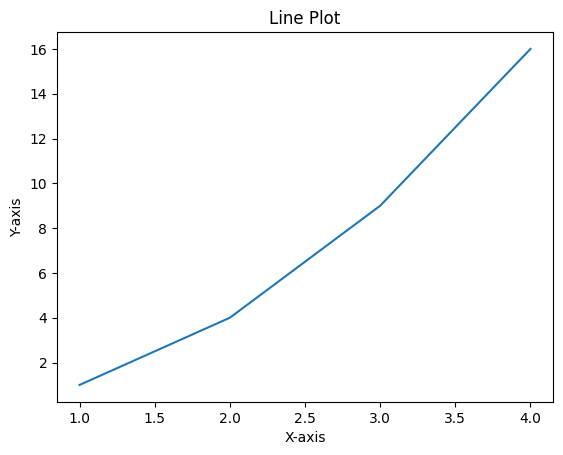
\includegraphics{cnu_data_handling_files/figure-pdf/cell-23-output-1.png}

\begin{Shaded}
\begin{Highlighting}[]
\ImportTok{import}\NormalTok{ matplotlib.pyplot }\ImportTok{as}\NormalTok{ plt}
\ImportTok{import}\NormalTok{ seaborn }\ImportTok{as}\NormalTok{ sns}

\NormalTok{data }\OperatorTok{=}\NormalTok{ [}
\NormalTok{    \{}\StringTok{\textquotesingle{}Name\textquotesingle{}}\NormalTok{: }\StringTok{\textquotesingle{}Alice\textquotesingle{}}\NormalTok{, }\StringTok{\textquotesingle{}Age\textquotesingle{}}\NormalTok{: }\DecValTok{25}\NormalTok{, }\StringTok{\textquotesingle{}Height\textquotesingle{}}\NormalTok{: }\FloatTok{5.5}\NormalTok{\},}
\NormalTok{    \{}\StringTok{\textquotesingle{}Name\textquotesingle{}}\NormalTok{: }\StringTok{\textquotesingle{}Bob\textquotesingle{}}\NormalTok{, }\StringTok{\textquotesingle{}Age\textquotesingle{}}\NormalTok{: }\DecValTok{30}\NormalTok{, }\StringTok{\textquotesingle{}Height\textquotesingle{}}\NormalTok{: }\FloatTok{6.0}\NormalTok{\},}
\NormalTok{    \{}\StringTok{\textquotesingle{}Name\textquotesingle{}}\NormalTok{: }\StringTok{\textquotesingle{}Charlie\textquotesingle{}}\NormalTok{, }\StringTok{\textquotesingle{}Age\textquotesingle{}}\NormalTok{: }\DecValTok{35}\NormalTok{, }\StringTok{\textquotesingle{}Height\textquotesingle{}}\NormalTok{: }\FloatTok{5.8}\NormalTok{\}}
\NormalTok{]}

\NormalTok{df }\OperatorTok{=}\NormalTok{ pd.DataFrame(data)}
\BuiltInTok{print}\NormalTok{(df)}

\CommentTok{\# Scatter plot with Seaborn}
\NormalTok{sns.scatterplot(x}\OperatorTok{=}\StringTok{\textquotesingle{}Age\textquotesingle{}}\NormalTok{, y}\OperatorTok{=}\StringTok{\textquotesingle{}Height\textquotesingle{}}\NormalTok{, data}\OperatorTok{=}\NormalTok{df)}
\NormalTok{plt.title(}\StringTok{\textquotesingle{}Age vs Height\textquotesingle{}}\NormalTok{)}
\NormalTok{plt.show()}
\end{Highlighting}
\end{Shaded}

\begin{verbatim}
      Name  Age  Height
0    Alice   25     5.5
1      Bob   30     6.0
2  Charlie   35     5.8
\end{verbatim}

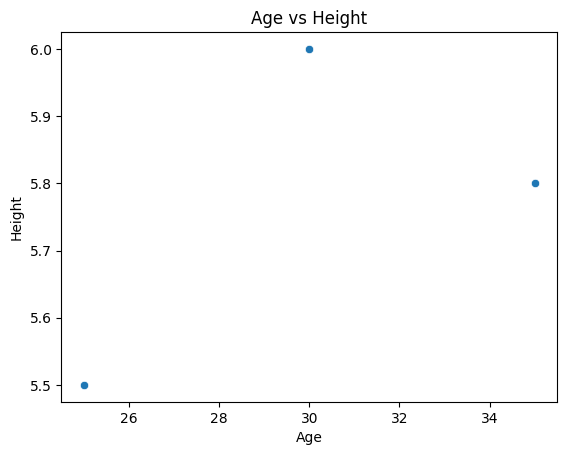
\includegraphics{cnu_data_handling_files/figure-pdf/cell-24-output-2.png}

\begin{Shaded}
\begin{Highlighting}[]
\BuiltInTok{dir}\NormalTok{(sns)}
\end{Highlighting}
\end{Shaded}

\subsection{Example: Analyzing and Visualizing DNA Sequence
Data}\label{example-analyzing-and-visualizing-dna-sequence-data}

\begin{figure}[H]

{\centering 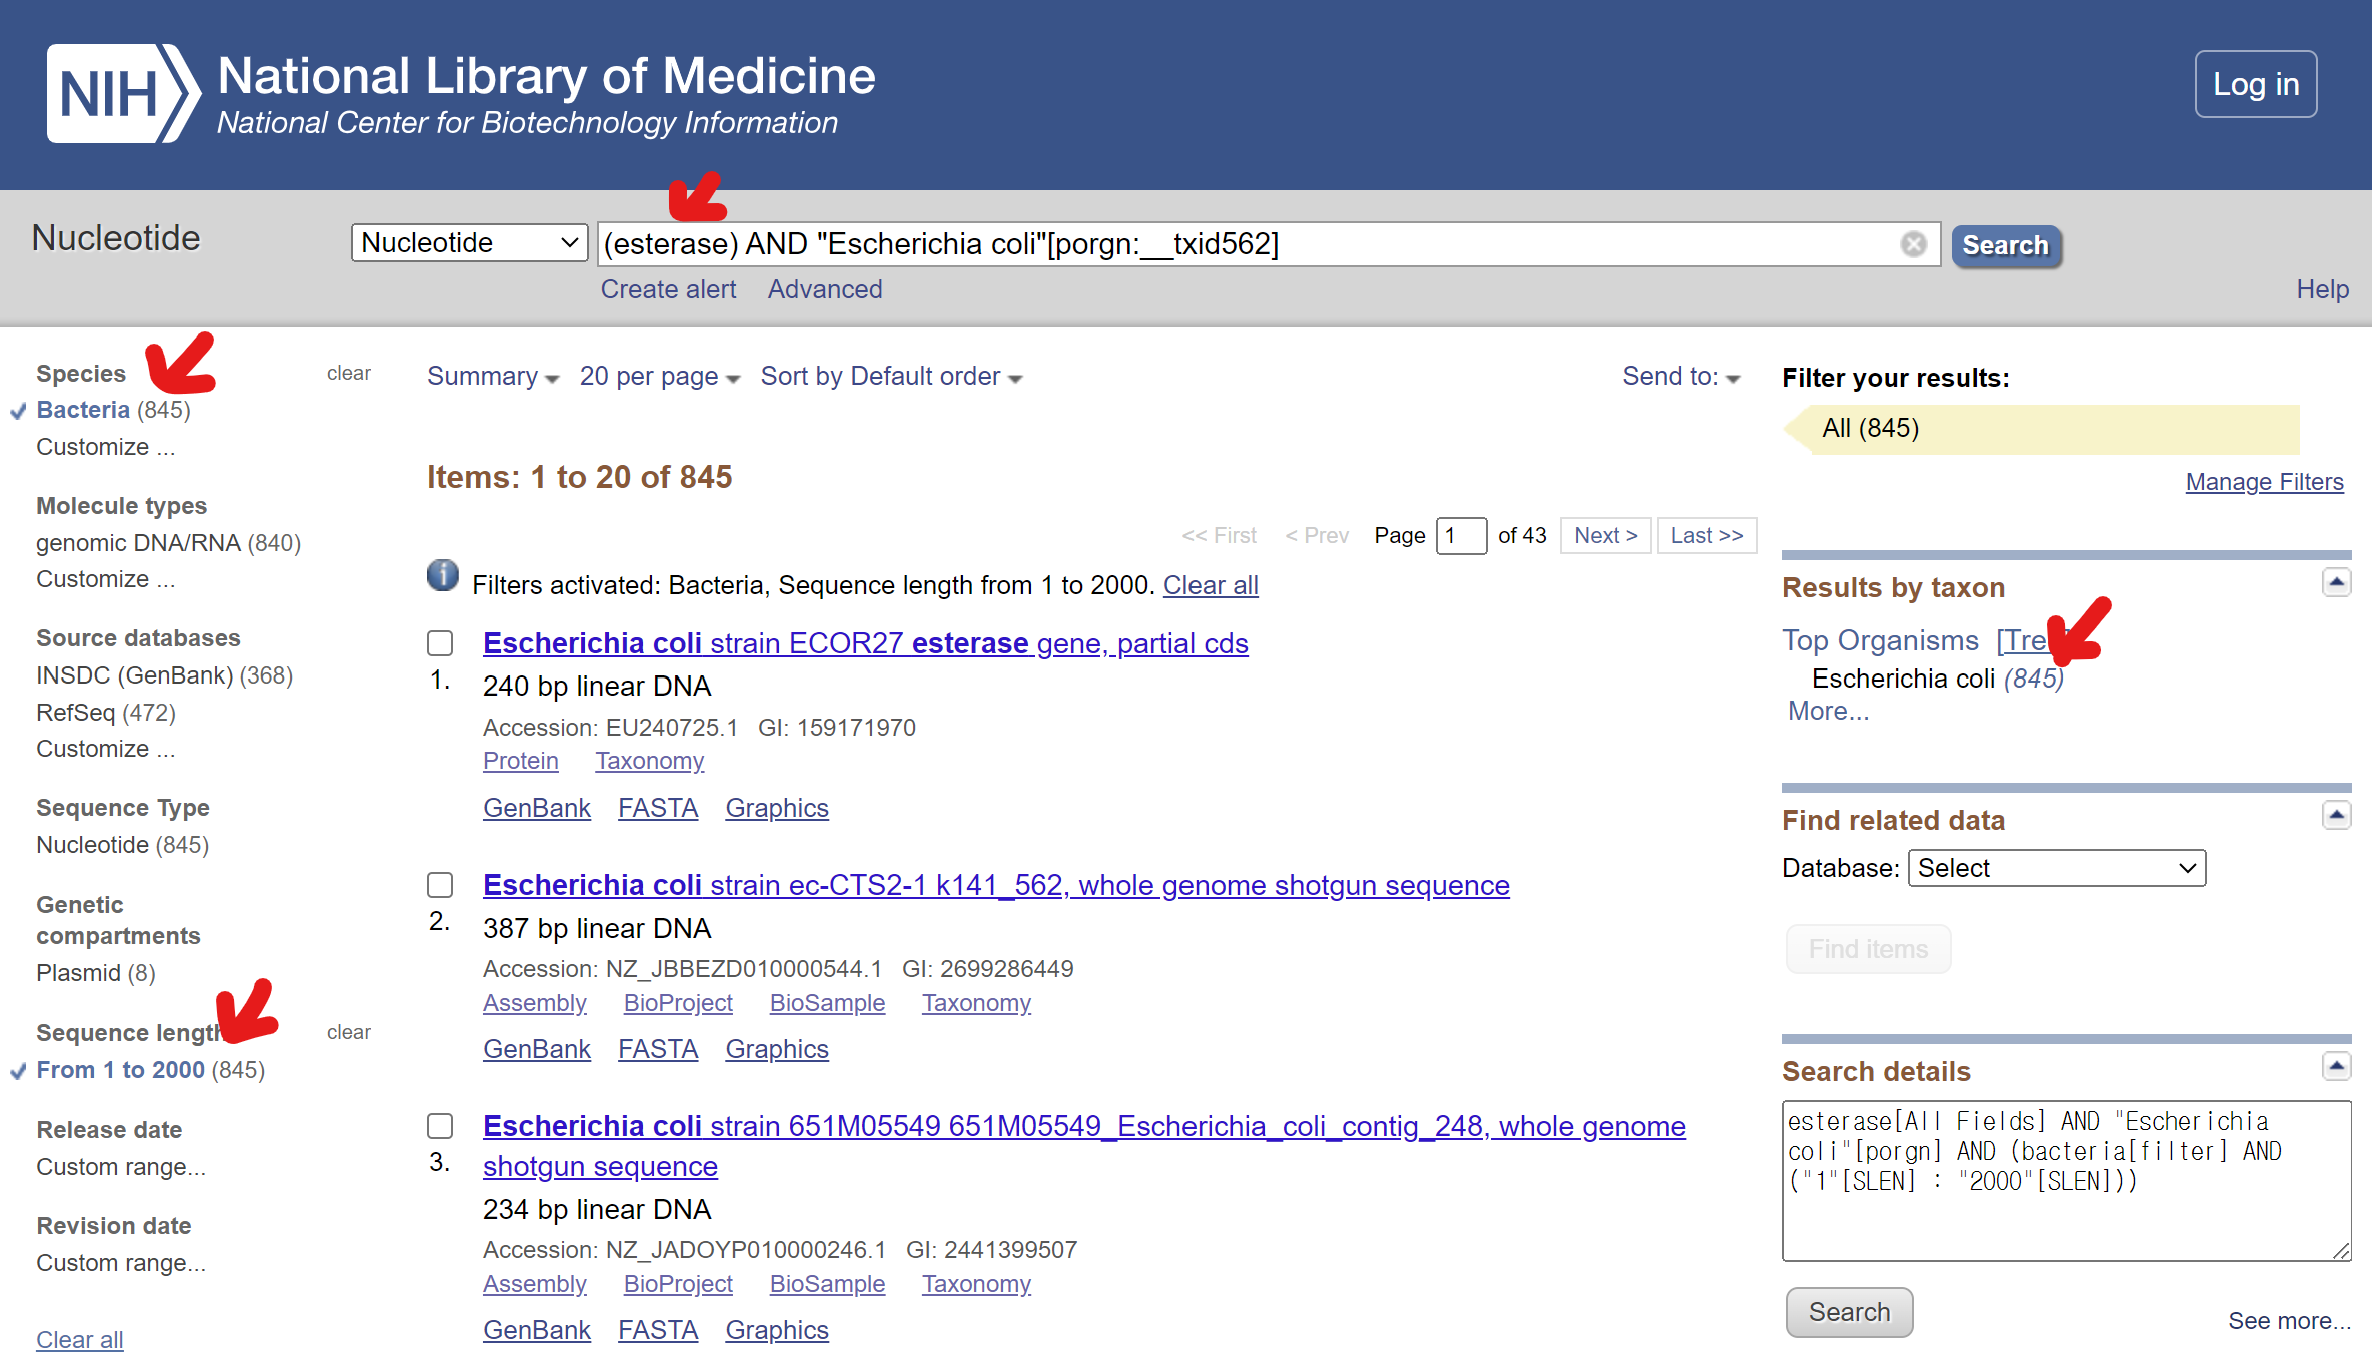
\includegraphics{images/ncbi_esterase2.png}

}

\caption{alt text}

\end{figure}%%
\begin{figure}[H]

{\centering 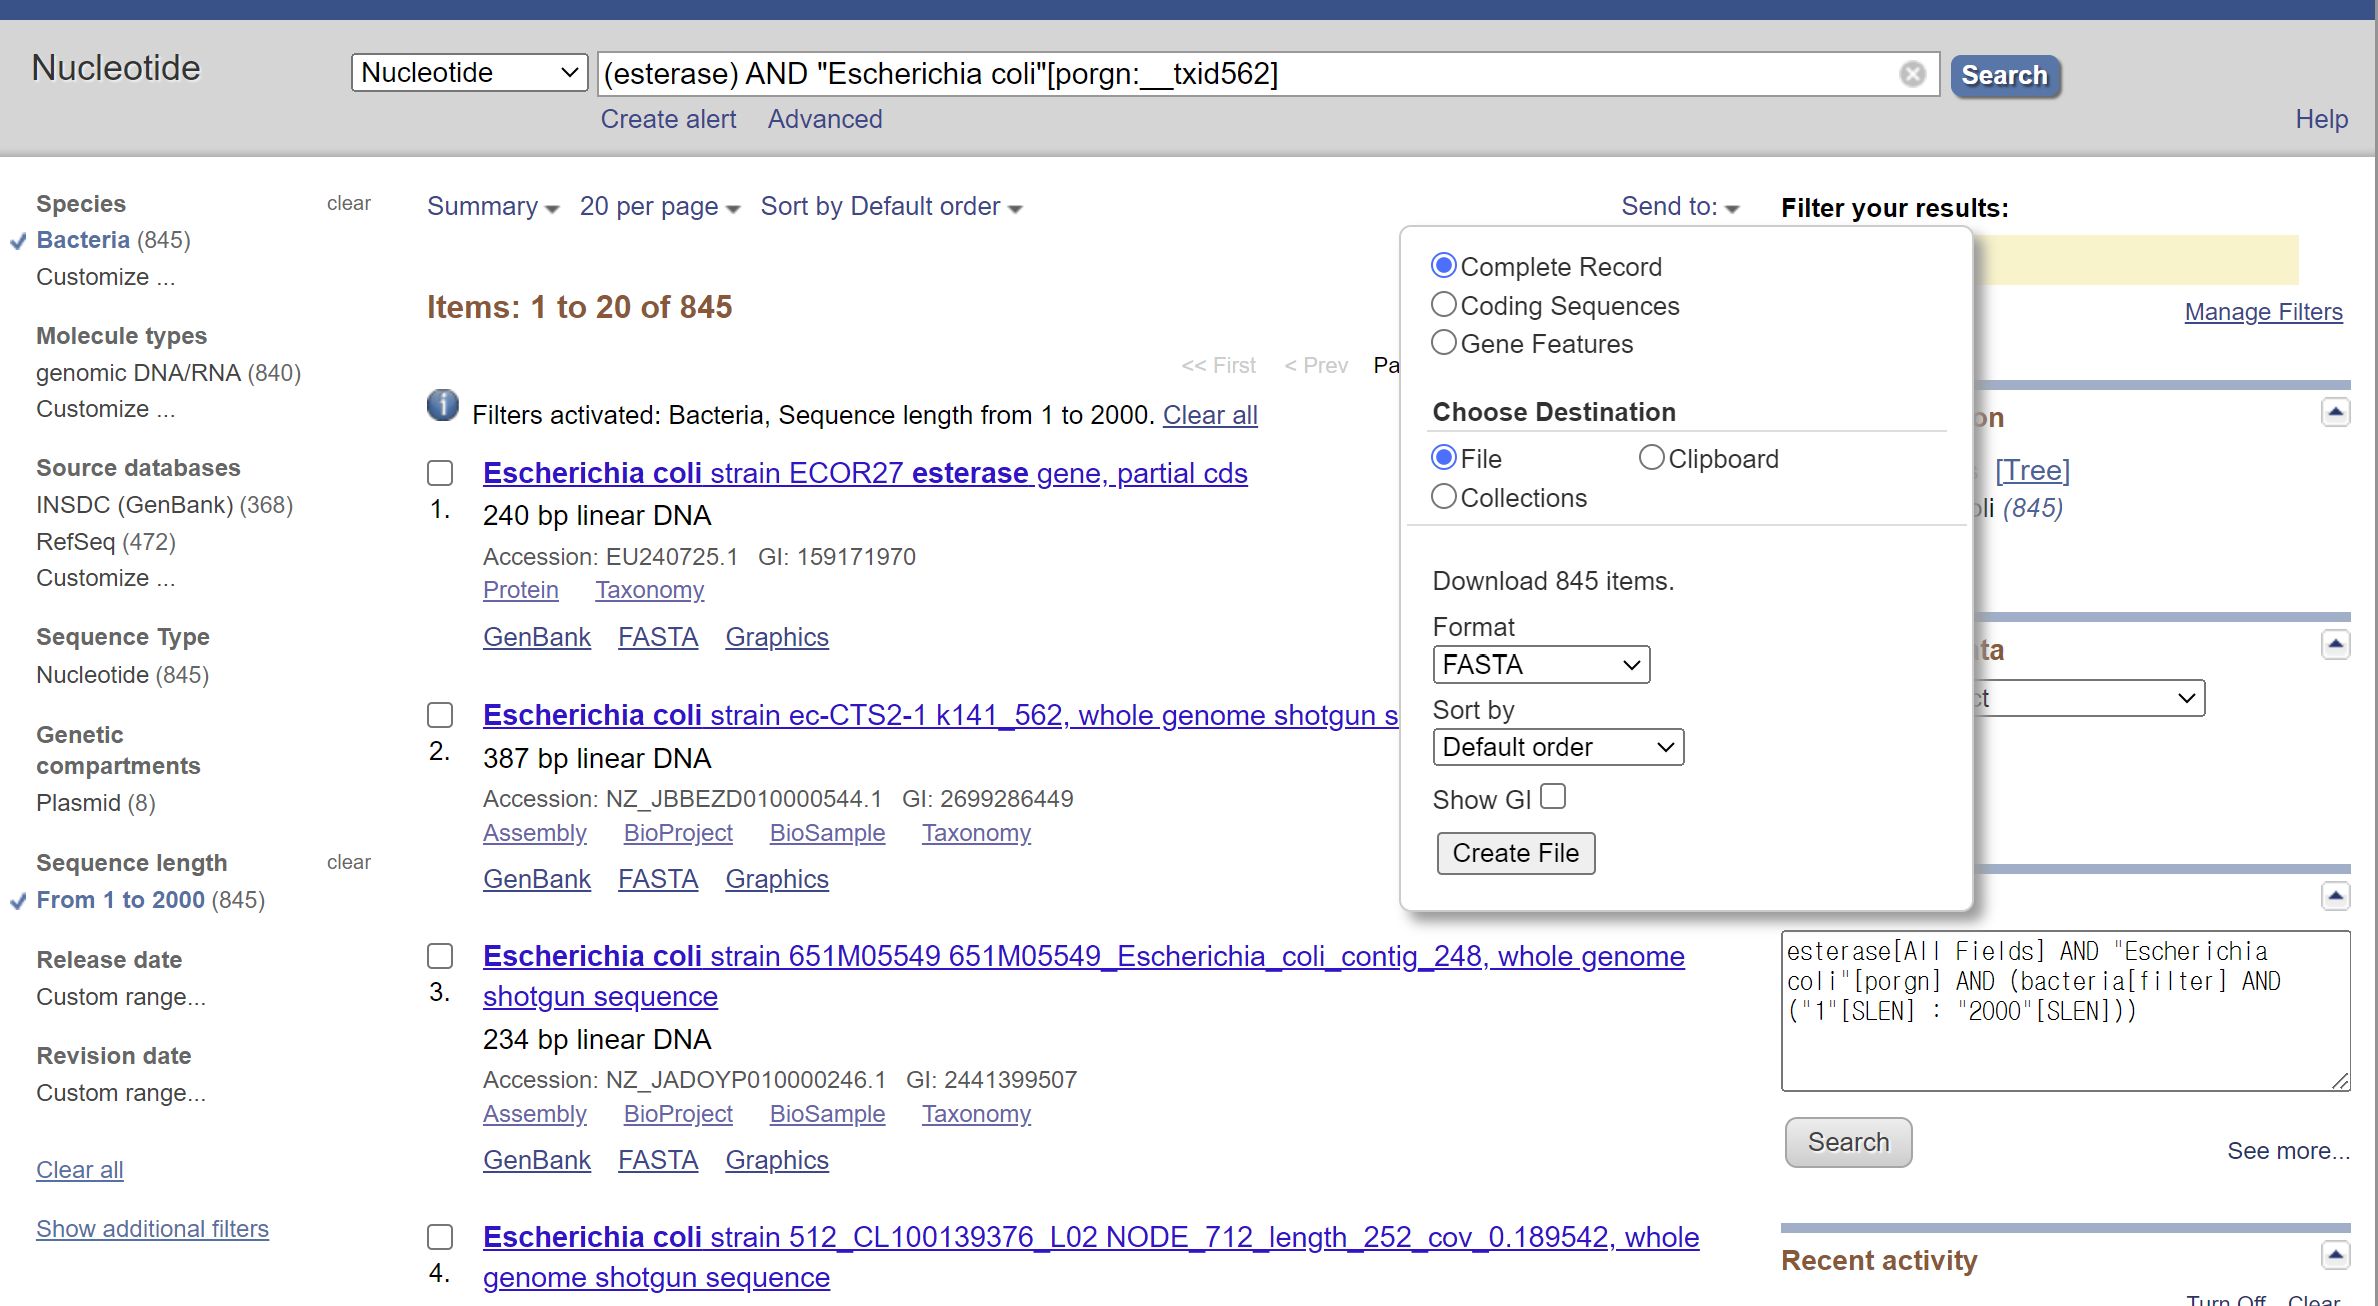
\includegraphics{images/ncbi_esterase_download_fasta.png}

}

\caption{alt text}

\end{figure}%

\subsubsection{{[}User{]}}\label{user-5}

{ I have downloaded a fasta file containing 800 esterase nucleotide
sequences. the file is saved at ``data/esterase.fa''. can you provide a
python code that can read the sequences and compute their length and GC
contents ratio? }

\subsubsection{{[}ChatGPT{]}}\label{chatgpt-5}

Certainly! To read a FASTA file containing 800 esterase nucleotide
sequences and compute their lengths and GC content ratios, you can use
the Biopython library. Here is a Python script that accomplishes this:

\textbf{Installation}

First, make sure you have Biopython installed:

\begin{Shaded}
\begin{Highlighting}[]
\ExtensionTok{pip}\NormalTok{ install biopython}
\end{Highlighting}
\end{Shaded}

\begin{Shaded}
\begin{Highlighting}[]
\ImportTok{from}\NormalTok{ Bio }\ImportTok{import}\NormalTok{ SeqIO}
\ImportTok{from}\NormalTok{ Bio.SeqUtils }\ImportTok{import}\NormalTok{ gc\_fraction}

\CommentTok{\# Function to compute sequence length and GC content}
\KeywordTok{def}\NormalTok{ compute\_sequence\_stats(seq):}
\NormalTok{    length }\OperatorTok{=} \BuiltInTok{len}\NormalTok{(seq)}
\NormalTok{    gc\_content }\OperatorTok{=}\NormalTok{ gc\_fraction(seq) }\OperatorTok{*} \DecValTok{100}  \CommentTok{\# Convert to percentage}
    \ControlFlowTok{return}\NormalTok{ length, gc\_content}

\CommentTok{\# Read the FASTA file and process each sequence}
\KeywordTok{def}\NormalTok{ process\_fasta\_file(file\_path):}
\NormalTok{    records }\OperatorTok{=}\NormalTok{ SeqIO.parse(file\_path, }\StringTok{"fasta"}\NormalTok{)}
\NormalTok{    esterase\_stats }\OperatorTok{=}\NormalTok{ []}

    \ControlFlowTok{for}\NormalTok{ record }\KeywordTok{in}\NormalTok{ records:}
\NormalTok{        length, gc\_content }\OperatorTok{=}\NormalTok{ compute\_sequence\_stats(record.seq)}
\NormalTok{        esterase\_stats.append(\{}
            \StringTok{"ID"}\NormalTok{: record.}\BuiltInTok{id}\NormalTok{,}
            \StringTok{"Length"}\NormalTok{: length,}
            \StringTok{"GC\_Content"}\NormalTok{: gc\_content}
\NormalTok{        \})}

    \ControlFlowTok{return}\NormalTok{ esterase\_stats}

\CommentTok{\# Example usage}
\NormalTok{fasta\_file }\OperatorTok{=} \StringTok{\textquotesingle{}data/esterases.fasta\textquotesingle{}}  \CommentTok{\# Replace with your FASTA file path}
\NormalTok{esterase\_stats }\OperatorTok{=}\NormalTok{ process\_fasta\_file(fasta\_file)}

\CommentTok{\# Print the results}
\ControlFlowTok{for}\NormalTok{ esterase }\KeywordTok{in}\NormalTok{ esterase\_stats:}
    \BuiltInTok{print}\NormalTok{(}\SpecialStringTok{f"ID: }\SpecialCharTok{\{}\NormalTok{esterase[}\StringTok{\textquotesingle{}ID\textquotesingle{}}\NormalTok{]}\SpecialCharTok{\}}\SpecialStringTok{, Length: }\SpecialCharTok{\{}\NormalTok{esterase[}\StringTok{\textquotesingle{}Length\textquotesingle{}}\NormalTok{]}\SpecialCharTok{\}}\SpecialStringTok{ bp, GC Content: }\SpecialCharTok{\{}\NormalTok{esterase[}\StringTok{\textquotesingle{}GC\_Content\textquotesingle{}}\NormalTok{]}\SpecialCharTok{:.2f\}}\SpecialStringTok{\%"}\NormalTok{)}
\end{Highlighting}
\end{Shaded}

\subsubsection{{[}User{]}}\label{user-6}

{ I want to store the result above in a file with json csv format. Than
I need a code to read the file and convert the data in a DataFrame
format. }

\subsubsection{{[}ChatGPT{]}}\label{chatgpt-6}

Sure! Let's modify the script to store the results in both JSON and CSV
formats. Then, we'll write a separate script to read these files and
convert the data into a Pandas DataFrame.

\begin{Shaded}
\begin{Highlighting}[]
\ImportTok{import}\NormalTok{ json}
\ImportTok{import}\NormalTok{ csv}
\ImportTok{from}\NormalTok{ Bio }\ImportTok{import}\NormalTok{ SeqIO}
\ImportTok{from}\NormalTok{ Bio.SeqUtils }\ImportTok{import}\NormalTok{ gc\_fraction}

\CommentTok{\# Function to compute sequence length and GC content}
\KeywordTok{def}\NormalTok{ compute\_sequence\_stats(seq):}
\NormalTok{    length }\OperatorTok{=} \BuiltInTok{len}\NormalTok{(seq)}
\NormalTok{    gc\_content }\OperatorTok{=}\NormalTok{ gc\_fraction(seq) }\OperatorTok{*} \DecValTok{100}  \CommentTok{\# Convert to percentage}
    \ControlFlowTok{return}\NormalTok{ length, gc\_content}

\CommentTok{\# Read the FASTA file and process each sequence}
\KeywordTok{def}\NormalTok{ process\_fasta\_file(file\_path):}
\NormalTok{    records }\OperatorTok{=}\NormalTok{ SeqIO.parse(file\_path, }\StringTok{"fasta"}\NormalTok{)}
\NormalTok{    esterase\_stats }\OperatorTok{=}\NormalTok{ []}

    \ControlFlowTok{for}\NormalTok{ record }\KeywordTok{in}\NormalTok{ records:}
\NormalTok{        length, gc\_content }\OperatorTok{=}\NormalTok{ compute\_sequence\_stats(record.seq)}
\NormalTok{        esterase\_stats.append(\{}
            \StringTok{"ID"}\NormalTok{: record.}\BuiltInTok{id}\NormalTok{,}
            \StringTok{"Length"}\NormalTok{: length,}
            \StringTok{"GC\_Content"}\NormalTok{: gc\_content}
\NormalTok{        \})}

    \ControlFlowTok{return}\NormalTok{ esterase\_stats}

\CommentTok{\# Save results to JSON and CSV}
\KeywordTok{def}\NormalTok{ save\_results(esterase\_stats, json\_file, csv\_file):}
    \CommentTok{\# Save to JSON}
    \ControlFlowTok{with} \BuiltInTok{open}\NormalTok{(json\_file, }\StringTok{\textquotesingle{}w\textquotesingle{}}\NormalTok{) }\ImportTok{as}\NormalTok{ jf:}
\NormalTok{        json.dump(esterase\_stats, jf, indent}\OperatorTok{=}\DecValTok{4}\NormalTok{)}

    \CommentTok{\# Save to CSV}
    \ControlFlowTok{with} \BuiltInTok{open}\NormalTok{(csv\_file, }\StringTok{\textquotesingle{}w\textquotesingle{}}\NormalTok{, newline}\OperatorTok{=}\StringTok{\textquotesingle{}\textquotesingle{}}\NormalTok{) }\ImportTok{as}\NormalTok{ cf:}
\NormalTok{        writer }\OperatorTok{=}\NormalTok{ csv.DictWriter(cf, fieldnames}\OperatorTok{=}\NormalTok{[}\StringTok{\textquotesingle{}ID\textquotesingle{}}\NormalTok{, }\StringTok{\textquotesingle{}Length\textquotesingle{}}\NormalTok{, }\StringTok{\textquotesingle{}GC\_Content\textquotesingle{}}\NormalTok{])}
\NormalTok{        writer.writeheader()}
        \ControlFlowTok{for}\NormalTok{ esterase }\KeywordTok{in}\NormalTok{ esterase\_stats:}
\NormalTok{            writer.writerow(esterase)}

\CommentTok{\# Example usage}
\NormalTok{fasta\_file }\OperatorTok{=} \StringTok{\textquotesingle{}data/esterases.fasta\textquotesingle{}}  \CommentTok{\# Replace with your FASTA file path}
\NormalTok{json\_file }\OperatorTok{=} \StringTok{\textquotesingle{}data/esterase\_stats.json\textquotesingle{}}
\NormalTok{csv\_file }\OperatorTok{=} \StringTok{\textquotesingle{}data/esterase\_stats.csv\textquotesingle{}}

\NormalTok{esterase\_stats }\OperatorTok{=}\NormalTok{ process\_fasta\_file(fasta\_file)}
\NormalTok{save\_results(esterase\_stats, json\_file, csv\_file)}

\BuiltInTok{print}\NormalTok{(}\SpecialStringTok{f"Results saved to }\SpecialCharTok{\{}\NormalTok{json\_file}\SpecialCharTok{\}}\SpecialStringTok{ and }\SpecialCharTok{\{}\NormalTok{csv\_file}\SpecialCharTok{\}}\SpecialStringTok{"}\NormalTok{)}
\end{Highlighting}
\end{Shaded}

\begin{verbatim}
Results saved to data/esterase_stats.json and data/esterase_stats.csv
\end{verbatim}

\begin{Shaded}
\begin{Highlighting}[]
\ImportTok{import}\NormalTok{ pandas }\ImportTok{as}\NormalTok{ pd}
\ImportTok{import}\NormalTok{ json}

\CommentTok{\# Load data from JSON file}
\ControlFlowTok{with} \BuiltInTok{open}\NormalTok{(}\StringTok{\textquotesingle{}data/esterase\_stats.json\textquotesingle{}}\NormalTok{, }\StringTok{\textquotesingle{}r\textquotesingle{}}\NormalTok{) }\ImportTok{as}\NormalTok{ jf:}
\NormalTok{    esterase\_stats\_json }\OperatorTok{=}\NormalTok{ json.load(jf)}

\CommentTok{\# Convert to DataFrame}
\NormalTok{df\_json }\OperatorTok{=}\NormalTok{ pd.DataFrame(esterase\_stats\_json)}
\BuiltInTok{print}\NormalTok{(}\StringTok{"DataFrame from JSON file:"}\NormalTok{)}
\BuiltInTok{print}\NormalTok{(df\_json.head())}

\CommentTok{\# Load data from CSV file}
\NormalTok{df\_csv }\OperatorTok{=}\NormalTok{ pd.read\_csv(}\StringTok{\textquotesingle{}data/esterase\_stats.csv\textquotesingle{}}\NormalTok{)}
\BuiltInTok{print}\NormalTok{(}\StringTok{"DataFrame from CSV file:"}\NormalTok{)}
\BuiltInTok{print}\NormalTok{(df\_csv.head())}
\end{Highlighting}
\end{Shaded}

\begin{verbatim}
DataFrame from JSON file:
                     ID  Length  GC_Content
0            EU240725.1     240   50.833333
1  NZ_JBBEZD010000544.1     387   48.062016
2  NZ_JADOYP010000246.1     234   55.982906
3  NZ_JAJAQZ010000712.1     252   52.777778
4  NZ_JABFYM010000640.1     769   52.405722
DataFrame from CSV file:
                     ID  Length  GC_Content
0            EU240725.1     240   50.833333
1  NZ_JBBEZD010000544.1     387   48.062016
2  NZ_JADOYP010000246.1     234   55.982906
3  NZ_JAJAQZ010000712.1     252   52.777778
4  NZ_JABFYM010000640.1     769   52.405722
\end{verbatim}

\subsubsection{{[}User{]}}\label{user-7}

{ I want a python code that display the statistics of the GC
distribution and boxplot of the length. }

\subsubsection{{[}ChatGPT{]}}\label{chatgpt-7}

Sure! Let's create a Python script that reads the data from the
previously saved JSON or CSV file, computes statistics for the GC
content distribution, and generates a boxplot for the sequence lengths
using Pandas and Matplotlib.

\begin{Shaded}
\begin{Highlighting}[]
\ImportTok{import}\NormalTok{ pandas }\ImportTok{as}\NormalTok{ pd}
\ImportTok{import}\NormalTok{ matplotlib.pyplot }\ImportTok{as}\NormalTok{ plt}
\ImportTok{import}\NormalTok{ seaborn }\ImportTok{as}\NormalTok{ sns}

\CommentTok{\# Load data from CSV file}
\NormalTok{df }\OperatorTok{=}\NormalTok{ pd.read\_csv(}\StringTok{\textquotesingle{}data/esterase\_stats.csv\textquotesingle{}}\NormalTok{)}

\CommentTok{\# Compute statistics for GC content distribution}
\NormalTok{gc\_stats }\OperatorTok{=}\NormalTok{ df[}\StringTok{\textquotesingle{}GC\_Content\textquotesingle{}}\NormalTok{].describe()}
\BuiltInTok{print}\NormalTok{(}\StringTok{"GC Content Distribution Statistics:"}\NormalTok{)}
\BuiltInTok{print}\NormalTok{(gc\_stats)}

\CommentTok{\# Generate a histogram for GC content distribution}
\NormalTok{plt.figure(figsize}\OperatorTok{=}\NormalTok{(}\DecValTok{10}\NormalTok{, }\DecValTok{6}\NormalTok{))}
\NormalTok{sns.histplot(df[}\StringTok{\textquotesingle{}GC\_Content\textquotesingle{}}\NormalTok{], bins}\OperatorTok{=}\DecValTok{30}\NormalTok{, kde}\OperatorTok{=}\VariableTok{True}\NormalTok{)}
\NormalTok{plt.title(}\StringTok{\textquotesingle{}GC Content Distribution\textquotesingle{}}\NormalTok{)}
\NormalTok{plt.xlabel(}\StringTok{\textquotesingle{}GC Content (\%)\textquotesingle{}}\NormalTok{)}
\NormalTok{plt.ylabel(}\StringTok{\textquotesingle{}Frequency\textquotesingle{}}\NormalTok{)}
\NormalTok{plt.show()}

\CommentTok{\# Generate a boxplot for sequence lengths}
\NormalTok{plt.figure(figsize}\OperatorTok{=}\NormalTok{(}\DecValTok{10}\NormalTok{, }\DecValTok{6}\NormalTok{))}
\NormalTok{sns.boxplot(x}\OperatorTok{=}\NormalTok{df[}\StringTok{\textquotesingle{}Length\textquotesingle{}}\NormalTok{])}
\NormalTok{plt.title(}\StringTok{\textquotesingle{}Boxplot of Sequence Lengths\textquotesingle{}}\NormalTok{)}
\NormalTok{plt.xlabel(}\StringTok{\textquotesingle{}Sequence Length (bp)\textquotesingle{}}\NormalTok{)}
\NormalTok{plt.show()}
\end{Highlighting}
\end{Shaded}

\begin{verbatim}
GC Content Distribution Statistics:
count    355.000000
mean      51.362399
std        5.551809
min       29.739777
25%       50.052780
50%       51.901566
75%       54.322222
max       75.683891
Name: GC_Content, dtype: float64
\end{verbatim}

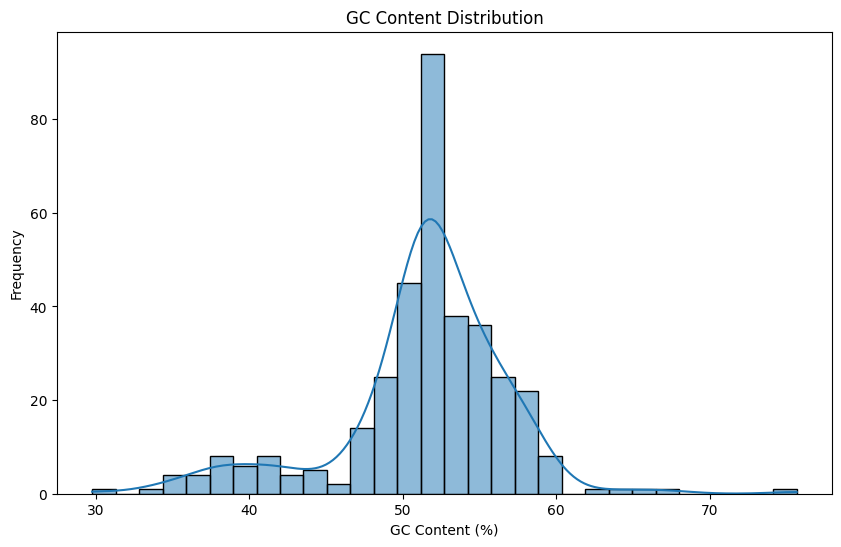
\includegraphics{cnu_data_handling_files/figure-pdf/cell-29-output-2.png}

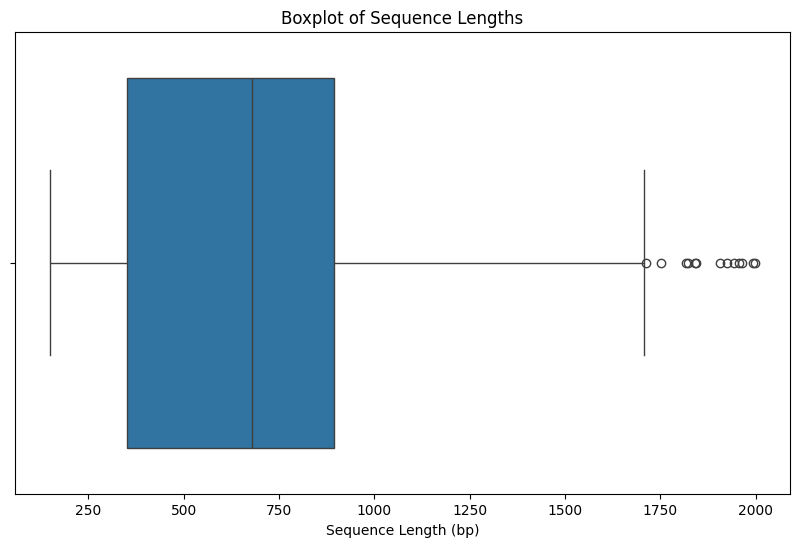
\includegraphics{cnu_data_handling_files/figure-pdf/cell-29-output-3.png}

\begin{itemize}
\tightlist
\item
  Script
\end{itemize}

\begin{Shaded}
\begin{Highlighting}[]
\ImportTok{from}\NormalTok{ Bio }\ImportTok{import}\NormalTok{ SeqIO}
\ImportTok{from}\NormalTok{ Bio.SeqUtils }\ImportTok{import}\NormalTok{ gc\_fraction}

\CommentTok{\# Read a FASTA file}
\NormalTok{fasta\_file }\OperatorTok{=} \StringTok{\textquotesingle{}data/esterases.fasta\textquotesingle{}}
\NormalTok{results }\OperatorTok{=}\NormalTok{ SeqIO.parse(fasta\_file, }\StringTok{\textquotesingle{}fasta\textquotesingle{}}\NormalTok{)}

\ControlFlowTok{for}\NormalTok{ record }\KeywordTok{in}\NormalTok{ results:}
    \BuiltInTok{print}\NormalTok{(record.}\BuiltInTok{id}\NormalTok{)}
    \BuiltInTok{print}\NormalTok{(record.seq)}
    \BuiltInTok{print}\NormalTok{(gc\_fraction(record.seq))}

\BuiltInTok{print}\NormalTok{(results)}
\end{Highlighting}
\end{Shaded}

\begin{itemize}
\tightlist
\item
  Calculate
\end{itemize}

\begin{Shaded}
\begin{Highlighting}[]
\ImportTok{from}\NormalTok{ Bio }\ImportTok{import}\NormalTok{ SeqIO}
\ImportTok{from}\NormalTok{ Bio.SeqUtils }\ImportTok{import}\NormalTok{ gc\_fraction}

\CommentTok{\# Read a FASTA file}
\NormalTok{fasta\_file }\OperatorTok{=} \StringTok{\textquotesingle{}data/esterases.fasta\textquotesingle{}}
\NormalTok{results }\OperatorTok{=}\NormalTok{ SeqIO.parse(fasta\_file, }\StringTok{\textquotesingle{}fasta\textquotesingle{}}\NormalTok{)}

\ControlFlowTok{for}\NormalTok{ record }\KeywordTok{in}\NormalTok{ results:}
\NormalTok{    seq }\OperatorTok{=}\NormalTok{ record.seq}
\NormalTok{    length }\OperatorTok{=} \BuiltInTok{len}\NormalTok{(seq)}
\NormalTok{    gc\_content }\OperatorTok{=}\NormalTok{ gc\_fraction(seq) }\OperatorTok{*} \DecValTok{100}  \CommentTok{\# Convert to percentage}
    \BuiltInTok{print}\NormalTok{(}\SpecialStringTok{f"ID: }\SpecialCharTok{\{}\NormalTok{record}\SpecialCharTok{.}\BuiltInTok{id}\SpecialCharTok{\}}\SpecialStringTok{, Length: }\SpecialCharTok{\{}\NormalTok{length}\SpecialCharTok{\}}\SpecialStringTok{ bp, GC Content: }\SpecialCharTok{\{}\NormalTok{gc\_content}\SpecialCharTok{:.2f\}}\SpecialStringTok{\%"}\NormalTok{)}
    
\end{Highlighting}
\end{Shaded}

\begin{itemize}
\tightlist
\item
  store in a list
\end{itemize}

\begin{Shaded}
\begin{Highlighting}[]
\ImportTok{from}\NormalTok{ Bio }\ImportTok{import}\NormalTok{ SeqIO}
\ImportTok{from}\NormalTok{ Bio.SeqUtils }\ImportTok{import}\NormalTok{ gc\_fraction}
\ImportTok{import}\NormalTok{ pandas }\ImportTok{as}\NormalTok{ pd}

\CommentTok{\# Read a FASTA file}
\NormalTok{fasta\_file }\OperatorTok{=} \StringTok{\textquotesingle{}data/esterases.fasta\textquotesingle{}}
\NormalTok{results }\OperatorTok{=}\NormalTok{ SeqIO.parse(fasta\_file, }\StringTok{\textquotesingle{}fasta\textquotesingle{}}\NormalTok{)}
\NormalTok{esterase\_stats }\OperatorTok{=}\NormalTok{ []}

\ControlFlowTok{for}\NormalTok{ record }\KeywordTok{in}\NormalTok{ results:}
\NormalTok{    seq }\OperatorTok{=}\NormalTok{ record.seq}
\NormalTok{    length }\OperatorTok{=} \BuiltInTok{len}\NormalTok{(seq)}
\NormalTok{    gc\_content }\OperatorTok{=}\NormalTok{ gc\_fraction(seq) }\OperatorTok{*} \DecValTok{100}  \CommentTok{\# Convert to percentage}
\NormalTok{    esterase\_stats.append(\{}
        \StringTok{"ID"}\NormalTok{: record.}\BuiltInTok{id}\NormalTok{,}
        \StringTok{"Length"}\NormalTok{: length,}
        \StringTok{"GC\_Content"}\NormalTok{: gc\_content}
\NormalTok{    \})}

\BuiltInTok{print}\NormalTok{(esterase\_stats) }
\NormalTok{pd.DataFrame(esterase\_stats)}
\end{Highlighting}
\end{Shaded}

\begin{itemize}
\tightlist
\item
  make a function
\end{itemize}

\begin{Shaded}
\begin{Highlighting}[]
\ImportTok{from}\NormalTok{ Bio }\ImportTok{import}\NormalTok{ SeqIO}
\ImportTok{from}\NormalTok{ Bio.SeqUtils }\ImportTok{import}\NormalTok{ gc\_fraction}
\ImportTok{import}\NormalTok{ pandas }\ImportTok{as}\NormalTok{ pd}

\CommentTok{\# Read a FASTA file}
\NormalTok{fasta\_file }\OperatorTok{=} \StringTok{\textquotesingle{}data/esterases.fasta\textquotesingle{}}
\NormalTok{results }\OperatorTok{=}\NormalTok{ SeqIO.parse(fasta\_file, }\StringTok{\textquotesingle{}fasta\textquotesingle{}}\NormalTok{)}
\NormalTok{esterase\_stats }\OperatorTok{=}\NormalTok{ []}

\CommentTok{\# Function to compute sequence length and GC content}
\KeywordTok{def}\NormalTok{ compute\_sequence\_stats(seq):}
\NormalTok{    length }\OperatorTok{=} \BuiltInTok{len}\NormalTok{(seq)}
\NormalTok{    gc\_content }\OperatorTok{=}\NormalTok{ gc\_fraction(seq) }\OperatorTok{*} \DecValTok{100}  \CommentTok{\# Convert to percentage}
    \ControlFlowTok{return}\NormalTok{ length, gc\_content}


\ControlFlowTok{for}\NormalTok{ record }\KeywordTok{in}\NormalTok{ results:}
\NormalTok{    seq }\OperatorTok{=}\NormalTok{ record.seq}
\NormalTok{    length, gc\_content }\OperatorTok{=}\NormalTok{ compute\_sequence\_stats(seq)}
\NormalTok{    esterase\_stats.append(\{}
        \StringTok{"ID"}\NormalTok{: record.}\BuiltInTok{id}\NormalTok{,}
        \StringTok{"Length"}\NormalTok{: length,}
        \StringTok{"GC\_Content"}\NormalTok{: gc\_content}
\NormalTok{    \})}

\BuiltInTok{print}\NormalTok{(esterase\_stats) }
\NormalTok{pd.DataFrame(esterase\_stats)}
\end{Highlighting}
\end{Shaded}

\bookmarksetup{startatroot}

\chapter{Bioinformatics}\label{bioinformatics}

\section{{[}User{]}}\label{user-8}

{ I want to learn about ``3. Bioinformatics Libraries''. Can you explain
it with example codes? }

\section{{[}ChatGPT{]}}\label{chatgpt-8}

Certainly! Bioinformatics libraries in Python, such as Biopython and
scikit-bio, provide tools and functions to handle biological data,
including sequence analysis, structure analysis, and more. Here's a
brief introduction to these libraries with example codes.

\section{Biopython}\label{biopython}

Biopython is one of the most widely used libraries for bioinformatics in
Python. It provides tools for reading and writing different
bioinformatics file formats, performing sequence analysis, and
interacting with biological databases.

\begin{Shaded}
\begin{Highlighting}[]
\ImportTok{from}\NormalTok{ google.colab }\ImportTok{import}\NormalTok{ drive}
\ImportTok{import}\NormalTok{ os}

\NormalTok{drive.mount(}\StringTok{\textquotesingle{}/content/drive\textquotesingle{}}\NormalTok{)}
\NormalTok{os.chdir(}\StringTok{\textquotesingle{}drive/MyDrive/2024{-}cnu{-}lecture\textquotesingle{}}\NormalTok{)}
\end{Highlighting}
\end{Shaded}

\begin{verbatim}
Mounted at /content/drive
\end{verbatim}

\subsection{Installation}\label{installation-1}

\begin{Shaded}
\begin{Highlighting}[]
\OperatorTok{!}\NormalTok{pip install biopython}
\end{Highlighting}
\end{Shaded}

\begin{verbatim}
Collecting biopython
  Downloading biopython-1.83-cp310-cp310-manylinux_2_17_x86_64.manylinux2014_x86_64.whl (3.1 MB)
     ━━━━━━━━━━━━━━━━━━━━━━━━━━━━━━━━━━━━━━━━ 3.1/3.1 MB 13.3 MB/s eta 0:00:00
Requirement already satisfied: numpy in /usr/local/lib/python3.10/dist-packages (from biopython) (1.25.2)
Installing collected packages: biopython
Successfully installed biopython-1.83
\end{verbatim}

\subsection{Sequence objects}\label{sequence-objects}

\begin{Shaded}
\begin{Highlighting}[]
\ImportTok{from}\NormalTok{ Bio.Seq }\ImportTok{import}\NormalTok{ Seq}
\NormalTok{my\_seq }\OperatorTok{=}\NormalTok{ Seq(}\StringTok{"AGTACACTGGT"}\NormalTok{)}
\NormalTok{my\_seq}
\end{Highlighting}
\end{Shaded}

\begin{verbatim}
Seq('AGTACACTGGT')
\end{verbatim}

\begin{Shaded}
\begin{Highlighting}[]
\ControlFlowTok{for}\NormalTok{ index, letter }\KeywordTok{in} \BuiltInTok{enumerate}\NormalTok{(my\_seq):}
    \BuiltInTok{print}\NormalTok{(}\StringTok{"}\SpecialCharTok{\%i}\StringTok{ }\SpecialCharTok{\%s}\StringTok{ "} \OperatorTok{\%}\NormalTok{ (index, letter))}
\end{Highlighting}
\end{Shaded}

\begin{verbatim}
0 A 
1 G 
2 T 
3 A 
4 C 
5 A 
6 C 
7 T 
8 G 
9 G 
10 T 
\end{verbatim}

\begin{Shaded}
\begin{Highlighting}[]
\NormalTok{x }\OperatorTok{=}\NormalTok{ [}\DecValTok{1}\NormalTok{, }\DecValTok{4}\NormalTok{, }\DecValTok{5}\NormalTok{, }\DecValTok{7}\NormalTok{, }\DecValTok{8}\NormalTok{]}
\ControlFlowTok{for}\NormalTok{ i }\KeywordTok{in} \BuiltInTok{enumerate}\NormalTok{(x):}
    \BuiltInTok{print}\NormalTok{(i)}

\ControlFlowTok{for}\NormalTok{ i }\KeywordTok{in}\NormalTok{ x:}
    \BuiltInTok{print}\NormalTok{(i)}
\end{Highlighting}
\end{Shaded}

\begin{verbatim}
(0, 1)
(1, 4)
(2, 5)
(3, 7)
(4, 8)
1
4
5
7
8
\end{verbatim}

\begin{Shaded}
\begin{Highlighting}[]
\BuiltInTok{print}\NormalTok{(my\_seq)}
\BuiltInTok{print}\NormalTok{(my\_seq[}\DecValTok{0}\NormalTok{:}\DecValTok{3}\NormalTok{])}
\BuiltInTok{print}\NormalTok{(my\_seq[}\DecValTok{0}\NormalTok{::}\DecValTok{2}\NormalTok{])}
\BuiltInTok{print}\NormalTok{(}\BuiltInTok{str}\NormalTok{(my\_seq))}
\BuiltInTok{print}\NormalTok{(my\_seq }\OperatorTok{+} \StringTok{"ATG"}\NormalTok{)}
\BuiltInTok{print}\NormalTok{(my\_seq}\OperatorTok{==}\StringTok{"ATG"}\NormalTok{)}
\BuiltInTok{print}\NormalTok{(}\StringTok{"AGT"} \KeywordTok{in}\NormalTok{ my\_seq)}
\end{Highlighting}
\end{Shaded}

\begin{verbatim}
AGTACACTGGT
AGT
ATCCGT
AGTACACTGGT
AGTACACTGGTATG
False
True
\end{verbatim}

\begin{Shaded}
\begin{Highlighting}[]
\NormalTok{my\_seq\_low }\OperatorTok{=}\NormalTok{ my\_seq.lower()}
\BuiltInTok{print}\NormalTok{(my\_seq\_low)}
\BuiltInTok{print}\NormalTok{(my\_seq\_low.upper())}
\BuiltInTok{print}\NormalTok{(my\_seq.complement())}
\BuiltInTok{print}\NormalTok{(my\_seq.reverse\_complement())}
\end{Highlighting}
\end{Shaded}

\begin{verbatim}
agtacactggt
AGTACACTGGT
TCATGTGACCA
ACCAGTGTACT
\end{verbatim}

\begin{itemize}
\tightlist
\item
  Transcription, Translation
\end{itemize}

\begin{Shaded}
\begin{Highlighting}[]
\NormalTok{mrna }\OperatorTok{=}\NormalTok{ my\_seq.transcribe()}
\BuiltInTok{print}\NormalTok{(mrna)}
\NormalTok{prot }\OperatorTok{=}\NormalTok{ mrna.translate() }\CommentTok{\#\# truncated}
\BuiltInTok{print}\NormalTok{(prot)}
\BuiltInTok{print}\NormalTok{(my\_seq.translate())}
\end{Highlighting}
\end{Shaded}

\begin{verbatim}
AGUACACUGGU
STL
STL
\end{verbatim}

\begin{verbatim}
/home/haseong/anaconda3/envs/biopy/lib/python3.11/site-packages/Bio/Seq.py:2880: BiopythonWarning: Partial codon, len(sequence) not a multiple of three. Explicitly trim the sequence or add trailing N before translation. This may become an error in future.
  warnings.warn(
\end{verbatim}

\begin{Shaded}
\begin{Highlighting}[]
\ImportTok{from}\NormalTok{ Bio.Data }\ImportTok{import}\NormalTok{ CodonTable}
\NormalTok{standard\_table }\OperatorTok{=}\NormalTok{ CodonTable.unambiguous\_dna\_by\_id[}\DecValTok{1}\NormalTok{]}
\BuiltInTok{print}\NormalTok{(standard\_table)}
\BuiltInTok{print}\NormalTok{(standard\_table.start\_codons)}
\BuiltInTok{print}\NormalTok{(standard\_table.stop\_codons)}
\BuiltInTok{print}\NormalTok{(}\BuiltInTok{type}\NormalTok{(standard\_table))}
\end{Highlighting}
\end{Shaded}

\begin{verbatim}
Table 1 Standard, SGC0

  |  T      |  C      |  A      |  G      |
--+---------+---------+---------+---------+--
T | TTT F   | TCT S   | TAT Y   | TGT C   | T
T | TTC F   | TCC S   | TAC Y   | TGC C   | C
T | TTA L   | TCA S   | TAA Stop| TGA Stop| A
T | TTG L(s)| TCG S   | TAG Stop| TGG W   | G
--+---------+---------+---------+---------+--
C | CTT L   | CCT P   | CAT H   | CGT R   | T
C | CTC L   | CCC P   | CAC H   | CGC R   | C
C | CTA L   | CCA P   | CAA Q   | CGA R   | A
C | CTG L(s)| CCG P   | CAG Q   | CGG R   | G
--+---------+---------+---------+---------+--
A | ATT I   | ACT T   | AAT N   | AGT S   | T
A | ATC I   | ACC T   | AAC N   | AGC S   | C
A | ATA I   | ACA T   | AAA K   | AGA R   | A
A | ATG M(s)| ACG T   | AAG K   | AGG R   | G
--+---------+---------+---------+---------+--
G | GTT V   | GCT A   | GAT D   | GGT G   | T
G | GTC V   | GCC A   | GAC D   | GGC G   | C
G | GTA V   | GCA A   | GAA E   | GGA G   | A
G | GTG V   | GCG A   | GAG E   | GGG G   | G
--+---------+---------+---------+---------+--
['TTG', 'CTG', 'ATG']
['TAA', 'TAG', 'TGA']
<class 'Bio.Data.CodonTable.NCBICodonTableDNA'>
\end{verbatim}

\begin{itemize}
\tightlist
\item
  MutableSeq objects
\end{itemize}

\begin{Shaded}
\begin{Highlighting}[]
\ImportTok{from}\NormalTok{ Bio.Seq }\ImportTok{import}\NormalTok{ Seq}
\NormalTok{my\_seq }\OperatorTok{=}\NormalTok{ Seq(}\StringTok{"AGTACACTGGT"}\NormalTok{)}
\NormalTok{my\_seq[}\DecValTok{5}\NormalTok{] }\OperatorTok{=} \StringTok{"G"}
\end{Highlighting}
\end{Shaded}

\begin{verbatim}
TypeError: 'Seq' object does not support item assignment
\end{verbatim}

\begin{Shaded}
\begin{Highlighting}[]
\ImportTok{from}\NormalTok{ Bio.Seq }\ImportTok{import}\NormalTok{ MutableSeq}

\NormalTok{mutable\_seq }\OperatorTok{=}\NormalTok{ MutableSeq(my\_seq)}
\NormalTok{mutable\_seq}

\NormalTok{mutable\_seq[}\DecValTok{5}\NormalTok{] }\OperatorTok{=} \StringTok{"G"}
\NormalTok{mutable\_seq}

\NormalTok{new\_seq }\OperatorTok{=}\NormalTok{ Seq(mutable\_seq)}
\NormalTok{new\_seq}
\end{Highlighting}
\end{Shaded}

\begin{verbatim}
Seq('AGTACGCTGGT')
\end{verbatim}

\begin{itemize}
\tightlist
\item
  Finding subsequence
\end{itemize}

\begin{Shaded}
\begin{Highlighting}[]
\NormalTok{seq }\OperatorTok{=}\NormalTok{ Seq(}\StringTok{"GCCATTGTAATGGGCCGCTGAAAGGGTGCCCGA"}\NormalTok{)}
\BuiltInTok{print}\NormalTok{(seq.index(}\StringTok{"ATG"}\NormalTok{))}
\BuiltInTok{print}\NormalTok{(seq.find(}\StringTok{"ATG"}\NormalTok{))}
\BuiltInTok{print}\NormalTok{(seq.find(}\StringTok{"AAAAA"}\NormalTok{))}
\end{Highlighting}
\end{Shaded}

\begin{verbatim}
9
9
-1
\end{verbatim}

\subsection{SeqRecord}\label{seqrecord}

\begin{itemize}
\tightlist
\item
  Sequence annotation objects
\item
  특정 서열의 identifier나 feature 정보 포함
\end{itemize}

\begin{Shaded}
\begin{Highlighting}[]
\ImportTok{from}\NormalTok{ Bio.Seq }\ImportTok{import}\NormalTok{ Seq}
\ImportTok{from}\NormalTok{ Bio.SeqRecord }\ImportTok{import}\NormalTok{ SeqRecord}

\NormalTok{simple\_seq }\OperatorTok{=}\NormalTok{ Seq(}\StringTok{"GATC"}\NormalTok{)}
\NormalTok{simple\_seq\_r }\OperatorTok{=}\NormalTok{ SeqRecord(simple\_seq)}
\end{Highlighting}
\end{Shaded}

\begin{Shaded}
\begin{Highlighting}[]
\BuiltInTok{help}\NormalTok{(SeqRecord)}
\end{Highlighting}
\end{Shaded}

\begin{verbatim}
Help on class SeqRecord in module Bio.SeqRecord:

class SeqRecord(builtins.object)
 |  SeqRecord(seq: Union[ForwardRef('Seq'), ForwardRef('MutableSeq'), NoneType], id: Optional[str] = '<unknown id>', name: str = '<unknown name>', description: str = '<unknown description>', dbxrefs: Optional[List[str]] = None, features: Optional[List[ForwardRef('SeqFeature')]] = None, annotations: Optional[Dict[str, Union[str, int]]] = None, letter_annotations: Optional[Dict[str, Sequence[Any]]] = None) -> None
 |  
 |  A SeqRecord object holds a sequence and information about it.
 |  
 |  Main attributes:
 |   - id          - Identifier such as a locus tag (string)
 |   - seq         - The sequence itself (Seq object or similar)
 |  
 |  Additional attributes:
 |   - name        - Sequence name, e.g. gene name (string)
 |   - description - Additional text (string)
 |   - dbxrefs     - List of database cross references (list of strings)
 |   - features    - Any (sub)features defined (list of SeqFeature objects)
 |   - annotations - Further information about the whole sequence (dictionary).
 |     Most entries are strings, or lists of strings.
 |   - letter_annotations - Per letter/symbol annotation (restricted
 |     dictionary). This holds Python sequences (lists, strings
 |     or tuples) whose length matches that of the sequence.
 |     A typical use would be to hold a list of integers
 |     representing sequencing quality scores, or a string
 |     representing the secondary structure.
 |  
 |  You will typically use Bio.SeqIO to read in sequences from files as
 |  SeqRecord objects.  However, you may want to create your own SeqRecord
 |  objects directly (see the __init__ method for further details):
 |  
 |  >>> from Bio.Seq import Seq
 |  >>> from Bio.SeqRecord import SeqRecord
 |  >>> record = SeqRecord(Seq("MKQHKAMIVALIVICITAVVAALVTRKDLCEVHIRTGQTEVAVF"),
 |  ...                    id="YP_025292.1", name="HokC",
 |  ...                    description="toxic membrane protein")
 |  >>> print(record)
 |  ID: YP_025292.1
 |  Name: HokC
 |  Description: toxic membrane protein
 |  Number of features: 0
 |  Seq('MKQHKAMIVALIVICITAVVAALVTRKDLCEVHIRTGQTEVAVF')
 |  
 |  If you want to save SeqRecord objects to a sequence file, use Bio.SeqIO
 |  for this.  For the special case where you want the SeqRecord turned into
 |  a string in a particular file format there is a format method which uses
 |  Bio.SeqIO internally:
 |  
 |  >>> print(record.format("fasta"))
 |  >YP_025292.1 toxic membrane protein
 |  MKQHKAMIVALIVICITAVVAALVTRKDLCEVHIRTGQTEVAVF
 |  <BLANKLINE>
 |  
 |  You can also do things like slicing a SeqRecord, checking its length, etc
 |  
 |  >>> len(record)
 |  44
 |  >>> edited = record[:10] + record[11:]
 |  >>> print(edited.seq)
 |  MKQHKAMIVAIVICITAVVAALVTRKDLCEVHIRTGQTEVAVF
 |  >>> print(record.seq)
 |  MKQHKAMIVALIVICITAVVAALVTRKDLCEVHIRTGQTEVAVF
 |  
 |  Methods defined here:
 |  
 |  __add__(self, other: Union[ForwardRef('SeqRecord'), ForwardRef('Seq'), ForwardRef('MutableSeq'), str]) -> 'SeqRecord'
 |      Add another sequence or string to this sequence.
 |      
 |      The other sequence can be a SeqRecord object, a Seq object (or
 |      similar, e.g. a MutableSeq) or a plain Python string. If you add
 |      a plain string or a Seq (like) object, the new SeqRecord will simply
 |      have this appended to the existing data. However, any per letter
 |      annotation will be lost:
 |      
 |      >>> from Bio import SeqIO
 |      >>> record = SeqIO.read("Quality/solexa_faked.fastq", "fastq-solexa")
 |      >>> print("%s %s" % (record.id, record.seq))
 |      slxa_0001_1_0001_01 ACGTACGTACGTACGTACGTACGTACGTACGTACGTACGTNNNNNN
 |      >>> print(list(record.letter_annotations))
 |      ['solexa_quality']
 |      
 |      >>> new = record + "ACT"
 |      >>> print("%s %s" % (new.id, new.seq))
 |      slxa_0001_1_0001_01 ACGTACGTACGTACGTACGTACGTACGTACGTACGTACGTNNNNNNACT
 |      >>> print(list(new.letter_annotations))
 |      []
 |      
 |      The new record will attempt to combine the annotation, but for any
 |      ambiguities (e.g. different names) it defaults to omitting that
 |      annotation.
 |      
 |      >>> from Bio import SeqIO
 |      >>> with open("GenBank/pBAD30.gb") as handle:
 |      ...     plasmid = SeqIO.read(handle, "gb")
 |      >>> print("%s %i" % (plasmid.id, len(plasmid)))
 |      pBAD30 4923
 |      
 |      Now let's cut the plasmid into two pieces, and join them back up the
 |      other way round (i.e. shift the starting point on this plasmid, have
 |      a look at the annotated features in the original file to see why this
 |      particular split point might make sense):
 |      
 |      >>> left = plasmid[:3765]
 |      >>> right = plasmid[3765:]
 |      >>> new = right + left
 |      >>> print("%s %i" % (new.id, len(new)))
 |      pBAD30 4923
 |      >>> str(new.seq) == str(right.seq + left.seq)
 |      True
 |      >>> len(new.features) == len(left.features) + len(right.features)
 |      True
 |      
 |      When we add the left and right SeqRecord objects, their annotation
 |      is all consistent, so it is all conserved in the new SeqRecord:
 |      
 |      >>> new.id == left.id == right.id == plasmid.id
 |      True
 |      >>> new.name == left.name == right.name == plasmid.name
 |      True
 |      >>> new.description == plasmid.description
 |      True
 |      >>> new.annotations == left.annotations == right.annotations
 |      True
 |      >>> new.letter_annotations == plasmid.letter_annotations
 |      True
 |      >>> new.dbxrefs == left.dbxrefs == right.dbxrefs
 |      True
 |      
 |      However, we should point out that when we sliced the SeqRecord,
 |      any annotations dictionary or dbxrefs list entries were lost.
 |      You can explicitly copy them like this:
 |      
 |      >>> new.annotations = plasmid.annotations.copy()
 |      >>> new.dbxrefs = plasmid.dbxrefs[:]
 |  
 |  __bool__(self) -> bool
 |      Boolean value of an instance of this class (True).
 |      
 |      This behaviour is for backwards compatibility, since until the
 |      __len__ method was added, a SeqRecord always evaluated as True.
 |      
 |      Note that in comparison, a Seq object will evaluate to False if it
 |      has a zero length sequence.
 |      
 |      WARNING: The SeqRecord may in future evaluate to False when its
 |      sequence is of zero length (in order to better match the Seq
 |      object behaviour)!
 |  
 |  __bytes__(self) -> bytes
 |  
 |  __contains__(self, char: str) -> bool
 |      Implement the 'in' keyword, searches the sequence.
 |      
 |      e.g.
 |      
 |      >>> from Bio import SeqIO
 |      >>> record = SeqIO.read("Fasta/sweetpea.nu", "fasta")
 |      >>> "GAATTC" in record
 |      False
 |      >>> "AAA" in record
 |      True
 |      
 |      This essentially acts as a proxy for using "in" on the sequence:
 |      
 |      >>> "GAATTC" in record.seq
 |      False
 |      >>> "AAA" in record.seq
 |      True
 |      
 |      Note that you can also use Seq objects as the query,
 |      
 |      >>> from Bio.Seq import Seq
 |      >>> Seq("AAA") in record
 |      True
 |      
 |      See also the Seq object's __contains__ method.
 |  
 |  __eq__(self, other: object) -> NoReturn
 |      Define the equal-to operand (not implemented).
 |  
 |  __format__(self, format_spec: str) -> str
 |      Return the record as a string in the specified file format.
 |      
 |      This method supports the Python format() function and f-strings.
 |      The format_spec should be a lower case string supported by
 |      Bio.SeqIO as a text output file format. Requesting a binary file
 |      format raises a ValueError. e.g.
 |      
 |      >>> from Bio.Seq import Seq
 |      >>> from Bio.SeqRecord import SeqRecord
 |      >>> record = SeqRecord(Seq("MKQHKAMIVALIVICITAVVAALVTRKDLCEVHIRTGQTEVAVF"),
 |      ...                    id="YP_025292.1", name="HokC",
 |      ...                    description="toxic membrane protein")
 |      ...
 |      >>> format(record, "fasta")
 |      '>YP_025292.1 toxic membrane protein\nMKQHKAMIVALIVICITAVVAALVTRKDLCEVHIRTGQTEVAVF\n'
 |      >>> print(f"Here is {record.id} in FASTA format:\n{record:fasta}")
 |      Here is YP_025292.1 in FASTA format:
 |      >YP_025292.1 toxic membrane protein
 |      MKQHKAMIVALIVICITAVVAALVTRKDLCEVHIRTGQTEVAVF
 |      <BLANKLINE>
 |      
 |      See also the SeqRecord's format() method.
 |  
 |  __ge__(self, other: Any) -> NoReturn
 |      Define the greater-than-or-equal-to operand (not implemented).
 |  
 |  __getitem__(self, index)
 |      Return a sub-sequence or an individual letter.
 |      
 |      Slicing, e.g. my_record[5:10], returns a new SeqRecord for
 |      that sub-sequence with some annotation preserved as follows:
 |      
 |      * The name, id and description are kept as-is.
 |      * Any per-letter-annotations are sliced to match the requested
 |        sub-sequence.
 |      * Unless a stride is used, all those features which fall fully
 |        within the subsequence are included (with their locations
 |        adjusted accordingly). If you want to preserve any truncated
 |        features (e.g. GenBank/EMBL source features), you must
 |        explicitly add them to the new SeqRecord yourself.
 |      * With the exception of any molecule type, the annotations
 |        dictionary and the dbxrefs list are not used for the new
 |        SeqRecord, as in general they may not apply to the
 |        subsequence. If you want to preserve them, you must explicitly
 |        copy them to the new SeqRecord yourself.
 |      
 |      Using an integer index, e.g. my_record[5] is shorthand for
 |      extracting that letter from the sequence, my_record.seq[5].
 |      
 |      For example, consider this short protein and its secondary
 |      structure as encoded by the PDB (e.g. H for alpha helices),
 |      plus a simple feature for its histidine self phosphorylation
 |      site:
 |      
 |      >>> from Bio.Seq import Seq
 |      >>> from Bio.SeqRecord import SeqRecord
 |      >>> from Bio.SeqFeature import SeqFeature, SimpleLocation
 |      >>> rec = SeqRecord(Seq("MAAGVKQLADDRTLLMAGVSHDLRTPLTRIRLAT"
 |      ...                     "EMMSEQDGYLAESINKDIEECNAIIEQFIDYLR"),
 |      ...                 id="1JOY", name="EnvZ",
 |      ...                 description="Homodimeric domain of EnvZ from E. coli")
 |      >>> rec.letter_annotations["secondary_structure"] = "  S  SSSSSSHHHHHTTTHHHHHHHHHHHHHHHHHHHHHHTHHHHHHHHHHHHHHHHHHHHHTT  "
 |      >>> rec.features.append(SeqFeature(SimpleLocation(20, 21),
 |      ...                     type = "Site"))
 |      
 |      Now let's have a quick look at the full record,
 |      
 |      >>> print(rec)
 |      ID: 1JOY
 |      Name: EnvZ
 |      Description: Homodimeric domain of EnvZ from E. coli
 |      Number of features: 1
 |      Per letter annotation for: secondary_structure
 |      Seq('MAAGVKQLADDRTLLMAGVSHDLRTPLTRIRLATEMMSEQDGYLAESINKDIEE...YLR')
 |      >>> rec.letter_annotations["secondary_structure"]
 |      '  S  SSSSSSHHHHHTTTHHHHHHHHHHHHHHHHHHHHHHTHHHHHHHHHHHHHHHHHHHHHTT  '
 |      >>> print(rec.features[0].location)
 |      [20:21]
 |      
 |      Now let's take a sub sequence, here chosen as the first (fractured)
 |      alpha helix which includes the histidine phosphorylation site:
 |      
 |      >>> sub = rec[11:41]
 |      >>> print(sub)
 |      ID: 1JOY
 |      Name: EnvZ
 |      Description: Homodimeric domain of EnvZ from E. coli
 |      Number of features: 1
 |      Per letter annotation for: secondary_structure
 |      Seq('RTLLMAGVSHDLRTPLTRIRLATEMMSEQD')
 |      >>> sub.letter_annotations["secondary_structure"]
 |      'HHHHHTTTHHHHHHHHHHHHHHHHHHHHHH'
 |      >>> print(sub.features[0].location)
 |      [9:10]
 |      
 |      You can also of course omit the start or end values, for
 |      example to get the first ten letters only:
 |      
 |      >>> print(rec[:10])
 |      ID: 1JOY
 |      Name: EnvZ
 |      Description: Homodimeric domain of EnvZ from E. coli
 |      Number of features: 0
 |      Per letter annotation for: secondary_structure
 |      Seq('MAAGVKQLAD')
 |      
 |      Or for the last ten letters:
 |      
 |      >>> print(rec[-10:])
 |      ID: 1JOY
 |      Name: EnvZ
 |      Description: Homodimeric domain of EnvZ from E. coli
 |      Number of features: 0
 |      Per letter annotation for: secondary_structure
 |      Seq('IIEQFIDYLR')
 |      
 |      If you omit both, then you get a copy of the original record (although
 |      lacking the annotations and dbxrefs):
 |      
 |      >>> print(rec[:])
 |      ID: 1JOY
 |      Name: EnvZ
 |      Description: Homodimeric domain of EnvZ from E. coli
 |      Number of features: 1
 |      Per letter annotation for: secondary_structure
 |      Seq('MAAGVKQLADDRTLLMAGVSHDLRTPLTRIRLATEMMSEQDGYLAESINKDIEE...YLR')
 |      
 |      Finally, indexing with a simple integer is shorthand for pulling out
 |      that letter from the sequence directly:
 |      
 |      >>> rec[5]
 |      'K'
 |      >>> rec.seq[5]
 |      'K'
 |  
 |  __gt__(self, other: Any) -> NoReturn
 |      Define the greater-than operand (not implemented).
 |  
 |  __init__(self, seq: Union[ForwardRef('Seq'), ForwardRef('MutableSeq'), NoneType], id: Optional[str] = '<unknown id>', name: str = '<unknown name>', description: str = '<unknown description>', dbxrefs: Optional[List[str]] = None, features: Optional[List[ForwardRef('SeqFeature')]] = None, annotations: Optional[Dict[str, Union[str, int]]] = None, letter_annotations: Optional[Dict[str, Sequence[Any]]] = None) -> None
 |      Create a SeqRecord.
 |      
 |      Arguments:
 |       - seq         - Sequence, required (Seq or MutableSeq)
 |       - id          - Sequence identifier, recommended (string)
 |       - name        - Sequence name, optional (string)
 |       - description - Sequence description, optional (string)
 |       - dbxrefs     - Database cross references, optional (list of strings)
 |       - features    - Any (sub)features, optional (list of SeqFeature objects)
 |       - annotations - Dictionary of annotations for the whole sequence
 |       - letter_annotations - Dictionary of per-letter-annotations, values
 |         should be strings, list or tuples of the same length as the full
 |         sequence.
 |      
 |      You will typically use Bio.SeqIO to read in sequences from files as
 |      SeqRecord objects.  However, you may want to create your own SeqRecord
 |      objects directly.
 |      
 |      Note that while an id is optional, we strongly recommend you supply a
 |      unique id string for each record.  This is especially important
 |      if you wish to write your sequences to a file.
 |      
 |      You can create a 'blank' SeqRecord object, and then populate the
 |      attributes later.
 |  
 |  __iter__(self) -> Iterable[Union[ForwardRef('Seq'), ForwardRef('MutableSeq')]]
 |      Iterate over the letters in the sequence.
 |      
 |      For example, using Bio.SeqIO to read in a protein FASTA file:
 |      
 |      >>> from Bio import SeqIO
 |      >>> record = SeqIO.read("Fasta/loveliesbleeding.pro", "fasta")
 |      >>> for amino in record:
 |      ...     print(amino)
 |      ...     if amino == "L": break
 |      X
 |      A
 |      G
 |      L
 |      >>> print(record.seq[3])
 |      L
 |      
 |      This is just a shortcut for iterating over the sequence directly:
 |      
 |      >>> for amino in record.seq:
 |      ...     print(amino)
 |      ...     if amino == "L": break
 |      X
 |      A
 |      G
 |      L
 |      >>> print(record.seq[3])
 |      L
 |      
 |      Note that this does not facilitate iteration together with any
 |      per-letter-annotation.  However, you can achieve that using the
 |      python zip function on the record (or its sequence) and the relevant
 |      per-letter-annotation:
 |      
 |      >>> from Bio import SeqIO
 |      >>> rec = SeqIO.read("Quality/solexa_faked.fastq", "fastq-solexa")
 |      >>> print("%s %s" % (rec.id, rec.seq))
 |      slxa_0001_1_0001_01 ACGTACGTACGTACGTACGTACGTACGTACGTACGTACGTNNNNNN
 |      >>> print(list(rec.letter_annotations))
 |      ['solexa_quality']
 |      >>> for nuc, qual in zip(rec, rec.letter_annotations["solexa_quality"]):
 |      ...     if qual > 35:
 |      ...         print("%s %i" % (nuc, qual))
 |      A 40
 |      C 39
 |      G 38
 |      T 37
 |      A 36
 |      
 |      You may agree that using zip(rec.seq, ...) is more explicit than using
 |      zip(rec, ...) as shown above.
 |  
 |  __le__(self, other: Any) -> NoReturn
 |      Define the less-than-or-equal-to operand (not implemented).
 |  
 |  __len__(self) -> int
 |      Return the length of the sequence.
 |      
 |      For example, using Bio.SeqIO to read in a FASTA nucleotide file:
 |      
 |      >>> from Bio import SeqIO
 |      >>> record = SeqIO.read("Fasta/sweetpea.nu", "fasta")
 |      >>> len(record)
 |      309
 |      >>> len(record.seq)
 |      309
 |  
 |  __lt__(self, other: Any) -> NoReturn
 |      Define the less-than operand (not implemented).
 |  
 |  __ne__(self, other: object) -> NoReturn
 |      Define the not-equal-to operand (not implemented).
 |  
 |  __radd__(self, other: Union[ForwardRef('Seq'), ForwardRef('MutableSeq'), str]) -> 'SeqRecord'
 |      Add another sequence or string to this sequence (from the left).
 |      
 |      This method handles adding a Seq object (or similar, e.g. MutableSeq)
 |      or a plain Python string (on the left) to a SeqRecord (on the right).
 |      See the __add__ method for more details, but for example:
 |      
 |      >>> from Bio import SeqIO
 |      >>> record = SeqIO.read("Quality/solexa_faked.fastq", "fastq-solexa")
 |      >>> print("%s %s" % (record.id, record.seq))
 |      slxa_0001_1_0001_01 ACGTACGTACGTACGTACGTACGTACGTACGTACGTACGTNNNNNN
 |      >>> print(list(record.letter_annotations))
 |      ['solexa_quality']
 |      
 |      >>> new = "ACT" + record
 |      >>> print("%s %s" % (new.id, new.seq))
 |      slxa_0001_1_0001_01 ACTACGTACGTACGTACGTACGTACGTACGTACGTACGTACGTNNNNNN
 |      >>> print(list(new.letter_annotations))
 |      []
 |  
 |  __repr__(self) -> str
 |      Return a concise summary of the record for debugging (string).
 |      
 |      The python built in function repr works by calling the object's __repr__
 |      method.  e.g.
 |      
 |      >>> from Bio.Seq import Seq
 |      >>> from Bio.SeqRecord import SeqRecord
 |      >>> rec = SeqRecord(Seq("MASRGVNKVILVGNLGQDPEVRYMPNGGAVANITLATSESWRDKAT"
 |      ...                     "GEMKEQTEWHRVVLFGKLAEVASEYLRKGSQVYIEGQLRTRKWTDQ"
 |      ...                     "SGQDRYTTEVVVNVGGTMQMLGGRQGGGAPAGGNIGGGQPQGGWGQ"
 |      ...                     "PQQPQGGNQFSGGAQSRPQQSAPAAPSNEPPMDFDDDIPF"),
 |      ...                 id="NP_418483.1", name="b4059",
 |      ...                 description="ssDNA-binding protein",
 |      ...                 dbxrefs=["ASAP:13298", "GI:16131885", "GeneID:948570"])
 |      >>> print(repr(rec))
 |      SeqRecord(seq=Seq('MASRGVNKVILVGNLGQDPEVRYMPNGGAVANITLATSESWRDKATGEMKEQTE...IPF'), id='NP_418483.1', name='b4059', description='ssDNA-binding protein', dbxrefs=['ASAP:13298', 'GI:16131885', 'GeneID:948570'])
 |      
 |      At the python prompt you can also use this shorthand:
 |      
 |      >>> rec
 |      SeqRecord(seq=Seq('MASRGVNKVILVGNLGQDPEVRYMPNGGAVANITLATSESWRDKATGEMKEQTE...IPF'), id='NP_418483.1', name='b4059', description='ssDNA-binding protein', dbxrefs=['ASAP:13298', 'GI:16131885', 'GeneID:948570'])
 |      
 |      Note that long sequences are shown truncated. Also note that any
 |      annotations, letter_annotations and features are not shown (as they
 |      would lead to a very long string).
 |  
 |  __str__(self) -> str
 |      Return a human readable summary of the record and its annotation (string).
 |      
 |      The python built in function str works by calling the object's __str__
 |      method.  e.g.
 |      
 |      >>> from Bio.Seq import Seq
 |      >>> from Bio.SeqRecord import SeqRecord
 |      >>> record = SeqRecord(Seq("MKQHKAMIVALIVICITAVVAALVTRKDLCEVHIRTGQTEVAVF"),
 |      ...                    id="YP_025292.1", name="HokC",
 |      ...                    description="toxic membrane protein, small")
 |      >>> print(str(record))
 |      ID: YP_025292.1
 |      Name: HokC
 |      Description: toxic membrane protein, small
 |      Number of features: 0
 |      Seq('MKQHKAMIVALIVICITAVVAALVTRKDLCEVHIRTGQTEVAVF')
 |      
 |      In this example you don't actually need to call str explicitly, as the
 |      print command does this automatically:
 |      
 |      >>> print(record)
 |      ID: YP_025292.1
 |      Name: HokC
 |      Description: toxic membrane protein, small
 |      Number of features: 0
 |      Seq('MKQHKAMIVALIVICITAVVAALVTRKDLCEVHIRTGQTEVAVF')
 |      
 |      Note that long sequences are shown truncated.
 |  
 |  count(self, sub, start=None, end=None)
 |      Return the number of non-overlapping occurrences of sub in seq[start:end].
 |      
 |      Optional arguments start and end are interpreted as in slice notation.
 |      This method behaves as the count method of Python strings.
 |  
 |  format(self, format: str) -> str
 |      Return the record as a string in the specified file format.
 |      
 |      The format should be a lower case string supported as an output
 |      format by Bio.SeqIO, which is used to turn the SeqRecord into a
 |      string.  e.g.
 |      
 |      >>> from Bio.Seq import Seq
 |      >>> from Bio.SeqRecord import SeqRecord
 |      >>> record = SeqRecord(Seq("MKQHKAMIVALIVICITAVVAALVTRKDLCEVHIRTGQTEVAVF"),
 |      ...                    id="YP_025292.1", name="HokC",
 |      ...                    description="toxic membrane protein")
 |      >>> record.format("fasta")
 |      '>YP_025292.1 toxic membrane protein\nMKQHKAMIVALIVICITAVVAALVTRKDLCEVHIRTGQTEVAVF\n'
 |      >>> print(record.format("fasta"))
 |      >YP_025292.1 toxic membrane protein
 |      MKQHKAMIVALIVICITAVVAALVTRKDLCEVHIRTGQTEVAVF
 |      <BLANKLINE>
 |      
 |      The Python print function automatically appends a new line, meaning
 |      in this example a blank line is shown.  If you look at the string
 |      representation you can see there is a trailing new line (shown as
 |      slash n) which is important when writing to a file or if
 |      concatenating multiple sequence strings together.
 |      
 |      Note that this method will NOT work on every possible file format
 |      supported by Bio.SeqIO (e.g. some are for multiple sequences only,
 |      and binary formats are not supported).
 |  
 |  islower(self)
 |      Return True if all ASCII characters in the record's sequence are lowercase.
 |      
 |      If there are no cased characters, the method returns False.
 |  
 |  isupper(self)
 |      Return True if all ASCII characters in the record's sequence are uppercase.
 |      
 |      If there are no cased characters, the method returns False.
 |  
 |  lower(self) -> 'SeqRecord'
 |      Return a copy of the record with a lower case sequence.
 |      
 |      All the annotation is preserved unchanged. e.g.
 |      
 |      >>> from Bio import SeqIO
 |      >>> record = SeqIO.read("Fasta/aster.pro", "fasta")
 |      >>> print(record.format("fasta"))
 |      >gi|3298468|dbj|BAA31520.1| SAMIPF
 |      GGHVNPAVTFGAFVGGNITLLRGIVYIIAQLLGSTVACLLLKFVTNDMAVGVFSLSAGVG
 |      VTNALVFEIVMTFGLVYTVYATAIDPKKGSLGTIAPIAIGFIVGANI
 |      <BLANKLINE>
 |      >>> print(record.lower().format("fasta"))
 |      >gi|3298468|dbj|BAA31520.1| SAMIPF
 |      gghvnpavtfgafvggnitllrgivyiiaqllgstvaclllkfvtndmavgvfslsagvg
 |      vtnalvfeivmtfglvytvyataidpkkgslgtiapiaigfivgani
 |      <BLANKLINE>
 |      
 |      To take a more annotation rich example,
 |      
 |      >>> from Bio import SeqIO
 |      >>> old = SeqIO.read("EMBL/TRBG361.embl", "embl")
 |      >>> len(old.features)
 |      3
 |      >>> new = old.lower()
 |      >>> len(old.features) == len(new.features)
 |      True
 |      >>> old.annotations["organism"] == new.annotations["organism"]
 |      True
 |      >>> old.dbxrefs == new.dbxrefs
 |      True
 |  
 |  reverse_complement(self, id: bool = False, name: bool = False, description: bool = False, features: bool = True, annotations: bool = False, letter_annotations: bool = True, dbxrefs: bool = False) -> 'SeqRecord'
 |      Return new SeqRecord with reverse complement sequence.
 |      
 |      By default the new record does NOT preserve the sequence identifier,
 |      name, description, general annotation or database cross-references -
 |      these are unlikely to apply to the reversed sequence.
 |      
 |      You can specify the returned record's id, name and description as
 |      strings, or True to keep that of the parent, or False for a default.
 |      
 |      You can specify the returned record's features with a list of
 |      SeqFeature objects, or True to keep that of the parent, or False to
 |      omit them. The default is to keep the original features (with the
 |      strand and locations adjusted).
 |      
 |      You can also specify both the returned record's annotations and
 |      letter_annotations as dictionaries, True to keep that of the parent,
 |      or False to omit them. The default is to keep the original
 |      annotations (with the letter annotations reversed).
 |      
 |      To show what happens to the pre-letter annotations, consider an
 |      example Solexa variant FASTQ file with a single entry, which we'll
 |      read in as a SeqRecord:
 |      
 |      >>> from Bio import SeqIO
 |      >>> record = SeqIO.read("Quality/solexa_faked.fastq", "fastq-solexa")
 |      >>> print("%s %s" % (record.id, record.seq))
 |      slxa_0001_1_0001_01 ACGTACGTACGTACGTACGTACGTACGTACGTACGTACGTNNNNNN
 |      >>> print(list(record.letter_annotations))
 |      ['solexa_quality']
 |      >>> print(record.letter_annotations["solexa_quality"])
 |      [40, 39, 38, 37, 36, 35, 34, 33, 32, 31, 30, 29, 28, 27, 26, 25, 24, 23, 22, 21, 20, 19, 18, 17, 16, 15, 14, 13, 12, 11, 10, 9, 8, 7, 6, 5, 4, 3, 2, 1, 0, -1, -2, -3, -4, -5]
 |      
 |      Now take the reverse complement, here we explicitly give a new
 |      identifier (the old identifier with a suffix):
 |      
 |      >>> rc_record = record.reverse_complement(id=record.id + "_rc")
 |      >>> print("%s %s" % (rc_record.id, rc_record.seq))
 |      slxa_0001_1_0001_01_rc NNNNNNACGTACGTACGTACGTACGTACGTACGTACGTACGTACGT
 |      
 |      Notice that the per-letter-annotations have also been reversed,
 |      although this may not be appropriate for all cases.
 |      
 |      >>> print(rc_record.letter_annotations["solexa_quality"])
 |      [-5, -4, -3, -2, -1, 0, 1, 2, 3, 4, 5, 6, 7, 8, 9, 10, 11, 12, 13, 14, 15, 16, 17, 18, 19, 20, 21, 22, 23, 24, 25, 26, 27, 28, 29, 30, 31, 32, 33, 34, 35, 36, 37, 38, 39, 40]
 |      
 |      Now for the features, we need a different example. Parsing a GenBank
 |      file is probably the easiest way to get an nice example with features
 |      in it...
 |      
 |      >>> from Bio import SeqIO
 |      >>> with open("GenBank/pBAD30.gb") as handle:
 |      ...     plasmid = SeqIO.read(handle, "gb")
 |      >>> print("%s %i" % (plasmid.id, len(plasmid)))
 |      pBAD30 4923
 |      >>> plasmid.seq
 |      Seq('GCTAGCGGAGTGTATACTGGCTTACTATGTTGGCACTGATGAGGGTGTCAGTGA...ATG')
 |      >>> len(plasmid.features)
 |      13
 |      
 |      Now, let's take the reverse complement of this whole plasmid:
 |      
 |      >>> rc_plasmid = plasmid.reverse_complement(id=plasmid.id+"_rc")
 |      >>> print("%s %i" % (rc_plasmid.id, len(rc_plasmid)))
 |      pBAD30_rc 4923
 |      >>> rc_plasmid.seq
 |      Seq('CATGGGCAAATATTATACGCAAGGCGACAAGGTGCTGATGCCGCTGGCGATTCA...AGC')
 |      >>> len(rc_plasmid.features)
 |      13
 |      
 |      Let's compare the first CDS feature - it has gone from being the
 |      second feature (index 1) to the second last feature (index -2), its
 |      strand has changed, and the location switched round.
 |      
 |      >>> print(plasmid.features[1])
 |      type: CDS
 |      location: [1081:1960](-)
 |      qualifiers:
 |          Key: label, Value: ['araC']
 |          Key: note, Value: ['araC regulator of the arabinose BAD promoter']
 |          Key: vntifkey, Value: ['4']
 |      <BLANKLINE>
 |      >>> print(rc_plasmid.features[-2])
 |      type: CDS
 |      location: [2963:3842](+)
 |      qualifiers:
 |          Key: label, Value: ['araC']
 |          Key: note, Value: ['araC regulator of the arabinose BAD promoter']
 |          Key: vntifkey, Value: ['4']
 |      <BLANKLINE>
 |      
 |      You can check this new location, based on the length of the plasmid:
 |      
 |      >>> len(plasmid) - 1081
 |      3842
 |      >>> len(plasmid) - 1960
 |      2963
 |      
 |      Note that if the SeqFeature annotation includes any strand specific
 |      information (e.g. base changes for a SNP), this information is not
 |      amended, and would need correction after the reverse complement.
 |      
 |      Note trying to reverse complement a protein SeqRecord raises an
 |      exception:
 |      
 |      >>> from Bio.Seq import Seq
 |      >>> from Bio.SeqRecord import SeqRecord
 |      >>> protein_rec = SeqRecord(Seq("MAIVMGR"), id="Test",
 |      ...                         annotations={"molecule_type": "protein"})
 |      >>> protein_rec.reverse_complement()
 |      Traceback (most recent call last):
 |         ...
 |      ValueError: Proteins do not have complements!
 |      
 |      If you have RNA without any U bases, it must be annotated as RNA
 |      otherwise it will be treated as DNA by default with A mapped to T:
 |      
 |      >>> from Bio.Seq import Seq
 |      >>> from Bio.SeqRecord import SeqRecord
 |      >>> rna1 = SeqRecord(Seq("ACG"), id="Test")
 |      >>> rna2 = SeqRecord(Seq("ACG"), id="Test", annotations={"molecule_type": "RNA"})
 |      >>> print(rna1.reverse_complement(id="RC", description="unk").format("fasta"))
 |      >RC unk
 |      CGT
 |      <BLANKLINE>
 |      >>> print(rna2.reverse_complement(id="RC", description="RNA").format("fasta"))
 |      >RC RNA
 |      CGU
 |      <BLANKLINE>
 |      
 |      Also note you can reverse complement a SeqRecord using a MutableSeq:
 |      
 |      >>> from Bio.Seq import MutableSeq
 |      >>> from Bio.SeqRecord import SeqRecord
 |      >>> rec = SeqRecord(MutableSeq("ACGT"), id="Test")
 |      >>> rec.seq[0] = "T"
 |      >>> print("%s %s" % (rec.id, rec.seq))
 |      Test TCGT
 |      >>> rc = rec.reverse_complement(id=True)
 |      >>> print("%s %s" % (rc.id, rc.seq))
 |      Test ACGA
 |  
 |  translate(self, table: str = 'Standard', stop_symbol: str = '*', to_stop: bool = False, cds: bool = False, gap: Optional[str] = None, id: bool = False, name: bool = False, description: bool = False, features: bool = False, annotations: bool = False, letter_annotations: bool = False, dbxrefs: bool = False) -> 'SeqRecord'
 |      Return new SeqRecord with translated sequence.
 |      
 |      This calls the record's .seq.translate() method (which describes
 |      the translation related arguments, like table for the genetic code),
 |      
 |      By default the new record does NOT preserve the sequence identifier,
 |      name, description, general annotation or database cross-references -
 |      these are unlikely to apply to the translated sequence.
 |      
 |      You can specify the returned record's id, name and description as
 |      strings, or True to keep that of the parent, or False for a default.
 |      
 |      You can specify the returned record's features with a list of
 |      SeqFeature objects, or False (default) to omit them.
 |      
 |      You can also specify both the returned record's annotations and
 |      letter_annotations as dictionaries, True to keep that of the parent
 |      (annotations only), or False (default) to omit them.
 |      
 |      e.g. Loading a FASTA gene and translating it,
 |      
 |      >>> from Bio import SeqIO
 |      >>> gene_record = SeqIO.read("Fasta/sweetpea.nu", "fasta")
 |      >>> print(gene_record.format("fasta"))
 |      >gi|3176602|gb|U78617.1|LOU78617 Lathyrus odoratus phytochrome A (PHYA) gene, partial cds
 |      CAGGCTGCGCGGTTTCTATTTATGAAGAACAAGGTCCGTATGATAGTTGATTGTCATGCA
 |      AAACATGTGAAGGTTCTTCAAGACGAAAAACTCCCATTTGATTTGACTCTGTGCGGTTCG
 |      ACCTTAAGAGCTCCACATAGTTGCCATTTGCAGTACATGGCTAACATGGATTCAATTGCT
 |      TCATTGGTTATGGCAGTGGTCGTCAATGACAGCGATGAAGATGGAGATAGCCGTGACGCA
 |      GTTCTACCACAAAAGAAAAAGAGACTTTGGGGTTTGGTAGTTTGTCATAACACTACTCCG
 |      AGGTTTGTT
 |      <BLANKLINE>
 |      
 |      And now translating the record, specifying the new ID and description:
 |      
 |      >>> protein_record = gene_record.translate(table=11,
 |      ...                                        id="phya",
 |      ...                                        description="translation")
 |      >>> print(protein_record.format("fasta"))
 |      >phya translation
 |      QAARFLFMKNKVRMIVDCHAKHVKVLQDEKLPFDLTLCGSTLRAPHSCHLQYMANMDSIA
 |      SLVMAVVVNDSDEDGDSRDAVLPQKKKRLWGLVVCHNTTPRFV
 |      <BLANKLINE>
 |  
 |  upper(self) -> 'SeqRecord'
 |      Return a copy of the record with an upper case sequence.
 |      
 |      All the annotation is preserved unchanged. e.g.
 |      
 |      >>> from Bio.Seq import Seq
 |      >>> from Bio.SeqRecord import SeqRecord
 |      >>> record = SeqRecord(Seq("acgtACGT"), id="Test",
 |      ...                    description = "Made up for this example")
 |      >>> record.letter_annotations["phred_quality"] = [1, 2, 3, 4, 5, 6, 7, 8]
 |      >>> print(record.upper().format("fastq"))
 |      @Test Made up for this example
 |      ACGTACGT
 |      +
 |      "#$%&'()
 |      <BLANKLINE>
 |      
 |      Naturally, there is a matching lower method:
 |      
 |      >>> print(record.lower().format("fastq"))
 |      @Test Made up for this example
 |      acgtacgt
 |      +
 |      "#$%&'()
 |      <BLANKLINE>
 |  
 |  ----------------------------------------------------------------------
 |  Data descriptors defined here:
 |  
 |  __dict__
 |      dictionary for instance variables (if defined)
 |  
 |  __weakref__
 |      list of weak references to the object (if defined)
 |  
 |  letter_annotations
 |      Dictionary of per-letter-annotation for the sequence.
 |      
 |      For example, this can hold quality scores used in FASTQ or QUAL files.
 |      Consider this example using Bio.SeqIO to read in an example Solexa
 |      variant FASTQ file as a SeqRecord:
 |      
 |      >>> from Bio import SeqIO
 |      >>> record = SeqIO.read("Quality/solexa_faked.fastq", "fastq-solexa")
 |      >>> print("%s %s" % (record.id, record.seq))
 |      slxa_0001_1_0001_01 ACGTACGTACGTACGTACGTACGTACGTACGTACGTACGTNNNNNN
 |      >>> print(list(record.letter_annotations))
 |      ['solexa_quality']
 |      >>> print(record.letter_annotations["solexa_quality"])
 |      [40, 39, 38, 37, 36, 35, 34, 33, 32, 31, 30, 29, 28, 27, 26, 25, 24, 23, 22, 21, 20, 19, 18, 17, 16, 15, 14, 13, 12, 11, 10, 9, 8, 7, 6, 5, 4, 3, 2, 1, 0, -1, -2, -3, -4, -5]
 |      
 |      The letter_annotations get sliced automatically if you slice the
 |      parent SeqRecord, for example taking the last ten bases:
 |      
 |      >>> sub_record = record[-10:]
 |      >>> print("%s %s" % (sub_record.id, sub_record.seq))
 |      slxa_0001_1_0001_01 ACGTNNNNNN
 |      >>> print(sub_record.letter_annotations["solexa_quality"])
 |      [4, 3, 2, 1, 0, -1, -2, -3, -4, -5]
 |      
 |      Any python sequence (i.e. list, tuple or string) can be recorded in
 |      the SeqRecord's letter_annotations dictionary as long as the length
 |      matches that of the SeqRecord's sequence.  e.g.
 |      
 |      >>> len(sub_record.letter_annotations)
 |      1
 |      >>> sub_record.letter_annotations["dummy"] = "abcdefghij"
 |      >>> len(sub_record.letter_annotations)
 |      2
 |      
 |      You can delete entries from the letter_annotations dictionary as usual:
 |      
 |      >>> del sub_record.letter_annotations["solexa_quality"]
 |      >>> sub_record.letter_annotations
 |      {'dummy': 'abcdefghij'}
 |      
 |      You can completely clear the dictionary easily as follows:
 |      
 |      >>> sub_record.letter_annotations = {}
 |      >>> sub_record.letter_annotations
 |      {}
 |      
 |      Note that if replacing the record's sequence with a sequence of a
 |      different length you must first clear the letter_annotations dict.
 |  
 |  seq
 |      The sequence itself, as a Seq or MutableSeq object.
 |  
 |  ----------------------------------------------------------------------
 |  Data and other attributes defined here:
 |  
 |  __annotations__ = {'annotations': typing.Dict[str, typing.Union[str, i...
 |  
 |  __hash__ = None
\end{verbatim}

\begin{itemize}
\tightlist
\item
  class 개념 이해 필요
\end{itemize}

\begin{Shaded}
\begin{Highlighting}[]
\NormalTok{simple\_seq\_r.}\BuiltInTok{id} \OperatorTok{=} \StringTok{"AC12345"}
\NormalTok{simple\_seq\_r.description }\OperatorTok{=} \StringTok{"Made up sequence I wish I could write a paper about"}
\BuiltInTok{print}\NormalTok{(simple\_seq\_r.description)}
\BuiltInTok{print}\NormalTok{(simple\_seq\_r.seq)}
\end{Highlighting}
\end{Shaded}

\begin{verbatim}
Made up sequence I wish I could write a paper about
GATC
\end{verbatim}

\begin{itemize}
\tightlist
\item
  Read fasta file
\item
  https://www.ncbi.nlm.nih.gov/nuccore/MW015936.1
\item
  Zika virus isolate Zika virus/H.sapiens-tc/THA/2006/CVD\_06-020,
  complete genome
\end{itemize}

\begin{figure}[H]

{\centering 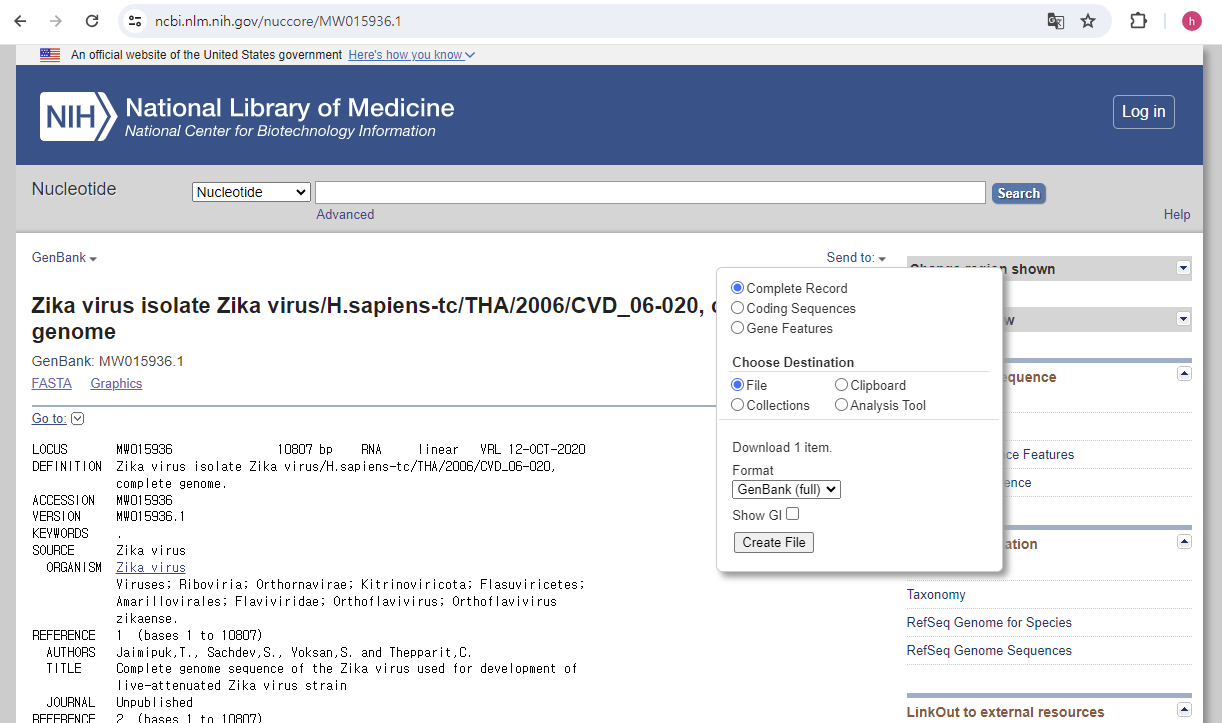
\includegraphics{images/zika.png}

}

\caption{alt text}

\end{figure}%

\begin{quote}
인용구 추가
\end{quote}

\begin{Shaded}
\begin{Highlighting}[]
\ImportTok{from}\NormalTok{ Bio }\ImportTok{import}\NormalTok{ SeqIO}
\NormalTok{record }\OperatorTok{=}\NormalTok{ SeqIO.read(}\StringTok{"data/MW015936.gb"}\NormalTok{, }\StringTok{"gb"}\NormalTok{)}
\end{Highlighting}
\end{Shaded}

\begin{Shaded}
\begin{Highlighting}[]
\BuiltInTok{print}\NormalTok{(record)}
\BuiltInTok{help}\NormalTok{(record)}
\end{Highlighting}
\end{Shaded}

\begin{verbatim}
ID: MW015936.1
Name: MW015936
Description: Zika virus isolate Zika virus/H.sapiens-tc/THA/2006/CVD_06-020, complete genome
Number of features: 17
/molecule_type=RNA
/topology=linear
/data_file_division=VRL
/date=12-OCT-2020
/accessions=['MW015936']
/sequence_version=1
/keywords=['']
/source=Zika virus
/organism=Zika virus
/taxonomy=['Viruses', 'Riboviria', 'Orthornavirae', 'Kitrinoviricota', 'Flasuviricetes', 'Amarillovirales', 'Flaviviridae', 'Orthoflavivirus', 'Orthoflavivirus zikaense']
/references=[Reference(title='Complete genome sequence of the Zika virus used for development of live-attenuated Zika virus strain', ...), Reference(title='Direct Submission', ...)]
/structured_comment=defaultdict(<class 'dict'>, {'Assembly-Data': {'Sequencing Technology': 'Sanger dideoxy sequencing'}})
Seq('AGTTGTTGATCTGTGTGAATCAGACTGCGACAGTTCGAGTTTGAAGCGAAAGCT...TCT')
Help on SeqRecord in module Bio.SeqRecord object:

class SeqRecord(builtins.object)
 |  SeqRecord(seq: Union[ForwardRef('Seq'), ForwardRef('MutableSeq'), NoneType], id: Optional[str] = '<unknown id>', name: str = '<unknown name>', description: str = '<unknown description>', dbxrefs: Optional[List[str]] = None, features: Optional[List[ForwardRef('SeqFeature')]] = None, annotations: Optional[Dict[str, Union[str, int]]] = None, letter_annotations: Optional[Dict[str, Sequence[Any]]] = None) -> None
 |  
 |  A SeqRecord object holds a sequence and information about it.
 |  
 |  Main attributes:
 |   - id          - Identifier such as a locus tag (string)
 |   - seq         - The sequence itself (Seq object or similar)
 |  
 |  Additional attributes:
 |   - name        - Sequence name, e.g. gene name (string)
 |   - description - Additional text (string)
 |   - dbxrefs     - List of database cross references (list of strings)
 |   - features    - Any (sub)features defined (list of SeqFeature objects)
 |   - annotations - Further information about the whole sequence (dictionary).
 |     Most entries are strings, or lists of strings.
 |   - letter_annotations - Per letter/symbol annotation (restricted
 |     dictionary). This holds Python sequences (lists, strings
 |     or tuples) whose length matches that of the sequence.
 |     A typical use would be to hold a list of integers
 |     representing sequencing quality scores, or a string
 |     representing the secondary structure.
 |  
 |  You will typically use Bio.SeqIO to read in sequences from files as
 |  SeqRecord objects.  However, you may want to create your own SeqRecord
 |  objects directly (see the __init__ method for further details):
 |  
 |  >>> from Bio.Seq import Seq
 |  >>> from Bio.SeqRecord import SeqRecord
 |  >>> record = SeqRecord(Seq("MKQHKAMIVALIVICITAVVAALVTRKDLCEVHIRTGQTEVAVF"),
 |  ...                    id="YP_025292.1", name="HokC",
 |  ...                    description="toxic membrane protein")
 |  >>> print(record)
 |  ID: YP_025292.1
 |  Name: HokC
 |  Description: toxic membrane protein
 |  Number of features: 0
 |  Seq('MKQHKAMIVALIVICITAVVAALVTRKDLCEVHIRTGQTEVAVF')
 |  
 |  If you want to save SeqRecord objects to a sequence file, use Bio.SeqIO
 |  for this.  For the special case where you want the SeqRecord turned into
 |  a string in a particular file format there is a format method which uses
 |  Bio.SeqIO internally:
 |  
 |  >>> print(record.format("fasta"))
 |  >YP_025292.1 toxic membrane protein
 |  MKQHKAMIVALIVICITAVVAALVTRKDLCEVHIRTGQTEVAVF
 |  <BLANKLINE>
 |  
 |  You can also do things like slicing a SeqRecord, checking its length, etc
 |  
 |  >>> len(record)
 |  44
 |  >>> edited = record[:10] + record[11:]
 |  >>> print(edited.seq)
 |  MKQHKAMIVAIVICITAVVAALVTRKDLCEVHIRTGQTEVAVF
 |  >>> print(record.seq)
 |  MKQHKAMIVALIVICITAVVAALVTRKDLCEVHIRTGQTEVAVF
 |  
 |  Methods defined here:
 |  
 |  __add__(self, other: Union[ForwardRef('SeqRecord'), ForwardRef('Seq'), ForwardRef('MutableSeq'), str]) -> 'SeqRecord'
 |      Add another sequence or string to this sequence.
 |      
 |      The other sequence can be a SeqRecord object, a Seq object (or
 |      similar, e.g. a MutableSeq) or a plain Python string. If you add
 |      a plain string or a Seq (like) object, the new SeqRecord will simply
 |      have this appended to the existing data. However, any per letter
 |      annotation will be lost:
 |      
 |      >>> from Bio import SeqIO
 |      >>> record = SeqIO.read("Quality/solexa_faked.fastq", "fastq-solexa")
 |      >>> print("%s %s" % (record.id, record.seq))
 |      slxa_0001_1_0001_01 ACGTACGTACGTACGTACGTACGTACGTACGTACGTACGTNNNNNN
 |      >>> print(list(record.letter_annotations))
 |      ['solexa_quality']
 |      
 |      >>> new = record + "ACT"
 |      >>> print("%s %s" % (new.id, new.seq))
 |      slxa_0001_1_0001_01 ACGTACGTACGTACGTACGTACGTACGTACGTACGTACGTNNNNNNACT
 |      >>> print(list(new.letter_annotations))
 |      []
 |      
 |      The new record will attempt to combine the annotation, but for any
 |      ambiguities (e.g. different names) it defaults to omitting that
 |      annotation.
 |      
 |      >>> from Bio import SeqIO
 |      >>> with open("GenBank/pBAD30.gb") as handle:
 |      ...     plasmid = SeqIO.read(handle, "gb")
 |      >>> print("%s %i" % (plasmid.id, len(plasmid)))
 |      pBAD30 4923
 |      
 |      Now let's cut the plasmid into two pieces, and join them back up the
 |      other way round (i.e. shift the starting point on this plasmid, have
 |      a look at the annotated features in the original file to see why this
 |      particular split point might make sense):
 |      
 |      >>> left = plasmid[:3765]
 |      >>> right = plasmid[3765:]
 |      >>> new = right + left
 |      >>> print("%s %i" % (new.id, len(new)))
 |      pBAD30 4923
 |      >>> str(new.seq) == str(right.seq + left.seq)
 |      True
 |      >>> len(new.features) == len(left.features) + len(right.features)
 |      True
 |      
 |      When we add the left and right SeqRecord objects, their annotation
 |      is all consistent, so it is all conserved in the new SeqRecord:
 |      
 |      >>> new.id == left.id == right.id == plasmid.id
 |      True
 |      >>> new.name == left.name == right.name == plasmid.name
 |      True
 |      >>> new.description == plasmid.description
 |      True
 |      >>> new.annotations == left.annotations == right.annotations
 |      True
 |      >>> new.letter_annotations == plasmid.letter_annotations
 |      True
 |      >>> new.dbxrefs == left.dbxrefs == right.dbxrefs
 |      True
 |      
 |      However, we should point out that when we sliced the SeqRecord,
 |      any annotations dictionary or dbxrefs list entries were lost.
 |      You can explicitly copy them like this:
 |      
 |      >>> new.annotations = plasmid.annotations.copy()
 |      >>> new.dbxrefs = plasmid.dbxrefs[:]
 |  
 |  __bool__(self) -> bool
 |      Boolean value of an instance of this class (True).
 |      
 |      This behaviour is for backwards compatibility, since until the
 |      __len__ method was added, a SeqRecord always evaluated as True.
 |      
 |      Note that in comparison, a Seq object will evaluate to False if it
 |      has a zero length sequence.
 |      
 |      WARNING: The SeqRecord may in future evaluate to False when its
 |      sequence is of zero length (in order to better match the Seq
 |      object behaviour)!
 |  
 |  __bytes__(self) -> bytes
 |  
 |  __contains__(self, char: str) -> bool
 |      Implement the 'in' keyword, searches the sequence.
 |      
 |      e.g.
 |      
 |      >>> from Bio import SeqIO
 |      >>> record = SeqIO.read("Fasta/sweetpea.nu", "fasta")
 |      >>> "GAATTC" in record
 |      False
 |      >>> "AAA" in record
 |      True
 |      
 |      This essentially acts as a proxy for using "in" on the sequence:
 |      
 |      >>> "GAATTC" in record.seq
 |      False
 |      >>> "AAA" in record.seq
 |      True
 |      
 |      Note that you can also use Seq objects as the query,
 |      
 |      >>> from Bio.Seq import Seq
 |      >>> Seq("AAA") in record
 |      True
 |      
 |      See also the Seq object's __contains__ method.
 |  
 |  __eq__(self, other: object) -> NoReturn
 |      Define the equal-to operand (not implemented).
 |  
 |  __format__(self, format_spec: str) -> str
 |      Return the record as a string in the specified file format.
 |      
 |      This method supports the Python format() function and f-strings.
 |      The format_spec should be a lower case string supported by
 |      Bio.SeqIO as a text output file format. Requesting a binary file
 |      format raises a ValueError. e.g.
 |      
 |      >>> from Bio.Seq import Seq
 |      >>> from Bio.SeqRecord import SeqRecord
 |      >>> record = SeqRecord(Seq("MKQHKAMIVALIVICITAVVAALVTRKDLCEVHIRTGQTEVAVF"),
 |      ...                    id="YP_025292.1", name="HokC",
 |      ...                    description="toxic membrane protein")
 |      ...
 |      >>> format(record, "fasta")
 |      '>YP_025292.1 toxic membrane protein\nMKQHKAMIVALIVICITAVVAALVTRKDLCEVHIRTGQTEVAVF\n'
 |      >>> print(f"Here is {record.id} in FASTA format:\n{record:fasta}")
 |      Here is YP_025292.1 in FASTA format:
 |      >YP_025292.1 toxic membrane protein
 |      MKQHKAMIVALIVICITAVVAALVTRKDLCEVHIRTGQTEVAVF
 |      <BLANKLINE>
 |      
 |      See also the SeqRecord's format() method.
 |  
 |  __ge__(self, other: Any) -> NoReturn
 |      Define the greater-than-or-equal-to operand (not implemented).
 |  
 |  __getitem__(self, index)
 |      Return a sub-sequence or an individual letter.
 |      
 |      Slicing, e.g. my_record[5:10], returns a new SeqRecord for
 |      that sub-sequence with some annotation preserved as follows:
 |      
 |      * The name, id and description are kept as-is.
 |      * Any per-letter-annotations are sliced to match the requested
 |        sub-sequence.
 |      * Unless a stride is used, all those features which fall fully
 |        within the subsequence are included (with their locations
 |        adjusted accordingly). If you want to preserve any truncated
 |        features (e.g. GenBank/EMBL source features), you must
 |        explicitly add them to the new SeqRecord yourself.
 |      * With the exception of any molecule type, the annotations
 |        dictionary and the dbxrefs list are not used for the new
 |        SeqRecord, as in general they may not apply to the
 |        subsequence. If you want to preserve them, you must explicitly
 |        copy them to the new SeqRecord yourself.
 |      
 |      Using an integer index, e.g. my_record[5] is shorthand for
 |      extracting that letter from the sequence, my_record.seq[5].
 |      
 |      For example, consider this short protein and its secondary
 |      structure as encoded by the PDB (e.g. H for alpha helices),
 |      plus a simple feature for its histidine self phosphorylation
 |      site:
 |      
 |      >>> from Bio.Seq import Seq
 |      >>> from Bio.SeqRecord import SeqRecord
 |      >>> from Bio.SeqFeature import SeqFeature, SimpleLocation
 |      >>> rec = SeqRecord(Seq("MAAGVKQLADDRTLLMAGVSHDLRTPLTRIRLAT"
 |      ...                     "EMMSEQDGYLAESINKDIEECNAIIEQFIDYLR"),
 |      ...                 id="1JOY", name="EnvZ",
 |      ...                 description="Homodimeric domain of EnvZ from E. coli")
 |      >>> rec.letter_annotations["secondary_structure"] = "  S  SSSSSSHHHHHTTTHHHHHHHHHHHHHHHHHHHHHHTHHHHHHHHHHHHHHHHHHHHHTT  "
 |      >>> rec.features.append(SeqFeature(SimpleLocation(20, 21),
 |      ...                     type = "Site"))
 |      
 |      Now let's have a quick look at the full record,
 |      
 |      >>> print(rec)
 |      ID: 1JOY
 |      Name: EnvZ
 |      Description: Homodimeric domain of EnvZ from E. coli
 |      Number of features: 1
 |      Per letter annotation for: secondary_structure
 |      Seq('MAAGVKQLADDRTLLMAGVSHDLRTPLTRIRLATEMMSEQDGYLAESINKDIEE...YLR')
 |      >>> rec.letter_annotations["secondary_structure"]
 |      '  S  SSSSSSHHHHHTTTHHHHHHHHHHHHHHHHHHHHHHTHHHHHHHHHHHHHHHHHHHHHTT  '
 |      >>> print(rec.features[0].location)
 |      [20:21]
 |      
 |      Now let's take a sub sequence, here chosen as the first (fractured)
 |      alpha helix which includes the histidine phosphorylation site:
 |      
 |      >>> sub = rec[11:41]
 |      >>> print(sub)
 |      ID: 1JOY
 |      Name: EnvZ
 |      Description: Homodimeric domain of EnvZ from E. coli
 |      Number of features: 1
 |      Per letter annotation for: secondary_structure
 |      Seq('RTLLMAGVSHDLRTPLTRIRLATEMMSEQD')
 |      >>> sub.letter_annotations["secondary_structure"]
 |      'HHHHHTTTHHHHHHHHHHHHHHHHHHHHHH'
 |      >>> print(sub.features[0].location)
 |      [9:10]
 |      
 |      You can also of course omit the start or end values, for
 |      example to get the first ten letters only:
 |      
 |      >>> print(rec[:10])
 |      ID: 1JOY
 |      Name: EnvZ
 |      Description: Homodimeric domain of EnvZ from E. coli
 |      Number of features: 0
 |      Per letter annotation for: secondary_structure
 |      Seq('MAAGVKQLAD')
 |      
 |      Or for the last ten letters:
 |      
 |      >>> print(rec[-10:])
 |      ID: 1JOY
 |      Name: EnvZ
 |      Description: Homodimeric domain of EnvZ from E. coli
 |      Number of features: 0
 |      Per letter annotation for: secondary_structure
 |      Seq('IIEQFIDYLR')
 |      
 |      If you omit both, then you get a copy of the original record (although
 |      lacking the annotations and dbxrefs):
 |      
 |      >>> print(rec[:])
 |      ID: 1JOY
 |      Name: EnvZ
 |      Description: Homodimeric domain of EnvZ from E. coli
 |      Number of features: 1
 |      Per letter annotation for: secondary_structure
 |      Seq('MAAGVKQLADDRTLLMAGVSHDLRTPLTRIRLATEMMSEQDGYLAESINKDIEE...YLR')
 |      
 |      Finally, indexing with a simple integer is shorthand for pulling out
 |      that letter from the sequence directly:
 |      
 |      >>> rec[5]
 |      'K'
 |      >>> rec.seq[5]
 |      'K'
 |  
 |  __gt__(self, other: Any) -> NoReturn
 |      Define the greater-than operand (not implemented).
 |  
 |  __init__(self, seq: Union[ForwardRef('Seq'), ForwardRef('MutableSeq'), NoneType], id: Optional[str] = '<unknown id>', name: str = '<unknown name>', description: str = '<unknown description>', dbxrefs: Optional[List[str]] = None, features: Optional[List[ForwardRef('SeqFeature')]] = None, annotations: Optional[Dict[str, Union[str, int]]] = None, letter_annotations: Optional[Dict[str, Sequence[Any]]] = None) -> None
 |      Create a SeqRecord.
 |      
 |      Arguments:
 |       - seq         - Sequence, required (Seq or MutableSeq)
 |       - id          - Sequence identifier, recommended (string)
 |       - name        - Sequence name, optional (string)
 |       - description - Sequence description, optional (string)
 |       - dbxrefs     - Database cross references, optional (list of strings)
 |       - features    - Any (sub)features, optional (list of SeqFeature objects)
 |       - annotations - Dictionary of annotations for the whole sequence
 |       - letter_annotations - Dictionary of per-letter-annotations, values
 |         should be strings, list or tuples of the same length as the full
 |         sequence.
 |      
 |      You will typically use Bio.SeqIO to read in sequences from files as
 |      SeqRecord objects.  However, you may want to create your own SeqRecord
 |      objects directly.
 |      
 |      Note that while an id is optional, we strongly recommend you supply a
 |      unique id string for each record.  This is especially important
 |      if you wish to write your sequences to a file.
 |      
 |      You can create a 'blank' SeqRecord object, and then populate the
 |      attributes later.
 |  
 |  __iter__(self) -> Iterable[Union[ForwardRef('Seq'), ForwardRef('MutableSeq')]]
 |      Iterate over the letters in the sequence.
 |      
 |      For example, using Bio.SeqIO to read in a protein FASTA file:
 |      
 |      >>> from Bio import SeqIO
 |      >>> record = SeqIO.read("Fasta/loveliesbleeding.pro", "fasta")
 |      >>> for amino in record:
 |      ...     print(amino)
 |      ...     if amino == "L": break
 |      X
 |      A
 |      G
 |      L
 |      >>> print(record.seq[3])
 |      L
 |      
 |      This is just a shortcut for iterating over the sequence directly:
 |      
 |      >>> for amino in record.seq:
 |      ...     print(amino)
 |      ...     if amino == "L": break
 |      X
 |      A
 |      G
 |      L
 |      >>> print(record.seq[3])
 |      L
 |      
 |      Note that this does not facilitate iteration together with any
 |      per-letter-annotation.  However, you can achieve that using the
 |      python zip function on the record (or its sequence) and the relevant
 |      per-letter-annotation:
 |      
 |      >>> from Bio import SeqIO
 |      >>> rec = SeqIO.read("Quality/solexa_faked.fastq", "fastq-solexa")
 |      >>> print("%s %s" % (rec.id, rec.seq))
 |      slxa_0001_1_0001_01 ACGTACGTACGTACGTACGTACGTACGTACGTACGTACGTNNNNNN
 |      >>> print(list(rec.letter_annotations))
 |      ['solexa_quality']
 |      >>> for nuc, qual in zip(rec, rec.letter_annotations["solexa_quality"]):
 |      ...     if qual > 35:
 |      ...         print("%s %i" % (nuc, qual))
 |      A 40
 |      C 39
 |      G 38
 |      T 37
 |      A 36
 |      
 |      You may agree that using zip(rec.seq, ...) is more explicit than using
 |      zip(rec, ...) as shown above.
 |  
 |  __le__(self, other: Any) -> NoReturn
 |      Define the less-than-or-equal-to operand (not implemented).
 |  
 |  __len__(self) -> int
 |      Return the length of the sequence.
 |      
 |      For example, using Bio.SeqIO to read in a FASTA nucleotide file:
 |      
 |      >>> from Bio import SeqIO
 |      >>> record = SeqIO.read("Fasta/sweetpea.nu", "fasta")
 |      >>> len(record)
 |      309
 |      >>> len(record.seq)
 |      309
 |  
 |  __lt__(self, other: Any) -> NoReturn
 |      Define the less-than operand (not implemented).
 |  
 |  __ne__(self, other: object) -> NoReturn
 |      Define the not-equal-to operand (not implemented).
 |  
 |  __radd__(self, other: Union[ForwardRef('Seq'), ForwardRef('MutableSeq'), str]) -> 'SeqRecord'
 |      Add another sequence or string to this sequence (from the left).
 |      
 |      This method handles adding a Seq object (or similar, e.g. MutableSeq)
 |      or a plain Python string (on the left) to a SeqRecord (on the right).
 |      See the __add__ method for more details, but for example:
 |      
 |      >>> from Bio import SeqIO
 |      >>> record = SeqIO.read("Quality/solexa_faked.fastq", "fastq-solexa")
 |      >>> print("%s %s" % (record.id, record.seq))
 |      slxa_0001_1_0001_01 ACGTACGTACGTACGTACGTACGTACGTACGTACGTACGTNNNNNN
 |      >>> print(list(record.letter_annotations))
 |      ['solexa_quality']
 |      
 |      >>> new = "ACT" + record
 |      >>> print("%s %s" % (new.id, new.seq))
 |      slxa_0001_1_0001_01 ACTACGTACGTACGTACGTACGTACGTACGTACGTACGTACGTNNNNNN
 |      >>> print(list(new.letter_annotations))
 |      []
 |  
 |  __repr__(self) -> str
 |      Return a concise summary of the record for debugging (string).
 |      
 |      The python built in function repr works by calling the object's __repr__
 |      method.  e.g.
 |      
 |      >>> from Bio.Seq import Seq
 |      >>> from Bio.SeqRecord import SeqRecord
 |      >>> rec = SeqRecord(Seq("MASRGVNKVILVGNLGQDPEVRYMPNGGAVANITLATSESWRDKAT"
 |      ...                     "GEMKEQTEWHRVVLFGKLAEVASEYLRKGSQVYIEGQLRTRKWTDQ"
 |      ...                     "SGQDRYTTEVVVNVGGTMQMLGGRQGGGAPAGGNIGGGQPQGGWGQ"
 |      ...                     "PQQPQGGNQFSGGAQSRPQQSAPAAPSNEPPMDFDDDIPF"),
 |      ...                 id="NP_418483.1", name="b4059",
 |      ...                 description="ssDNA-binding protein",
 |      ...                 dbxrefs=["ASAP:13298", "GI:16131885", "GeneID:948570"])
 |      >>> print(repr(rec))
 |      SeqRecord(seq=Seq('MASRGVNKVILVGNLGQDPEVRYMPNGGAVANITLATSESWRDKATGEMKEQTE...IPF'), id='NP_418483.1', name='b4059', description='ssDNA-binding protein', dbxrefs=['ASAP:13298', 'GI:16131885', 'GeneID:948570'])
 |      
 |      At the python prompt you can also use this shorthand:
 |      
 |      >>> rec
 |      SeqRecord(seq=Seq('MASRGVNKVILVGNLGQDPEVRYMPNGGAVANITLATSESWRDKATGEMKEQTE...IPF'), id='NP_418483.1', name='b4059', description='ssDNA-binding protein', dbxrefs=['ASAP:13298', 'GI:16131885', 'GeneID:948570'])
 |      
 |      Note that long sequences are shown truncated. Also note that any
 |      annotations, letter_annotations and features are not shown (as they
 |      would lead to a very long string).
 |  
 |  __str__(self) -> str
 |      Return a human readable summary of the record and its annotation (string).
 |      
 |      The python built in function str works by calling the object's __str__
 |      method.  e.g.
 |      
 |      >>> from Bio.Seq import Seq
 |      >>> from Bio.SeqRecord import SeqRecord
 |      >>> record = SeqRecord(Seq("MKQHKAMIVALIVICITAVVAALVTRKDLCEVHIRTGQTEVAVF"),
 |      ...                    id="YP_025292.1", name="HokC",
 |      ...                    description="toxic membrane protein, small")
 |      >>> print(str(record))
 |      ID: YP_025292.1
 |      Name: HokC
 |      Description: toxic membrane protein, small
 |      Number of features: 0
 |      Seq('MKQHKAMIVALIVICITAVVAALVTRKDLCEVHIRTGQTEVAVF')
 |      
 |      In this example you don't actually need to call str explicitly, as the
 |      print command does this automatically:
 |      
 |      >>> print(record)
 |      ID: YP_025292.1
 |      Name: HokC
 |      Description: toxic membrane protein, small
 |      Number of features: 0
 |      Seq('MKQHKAMIVALIVICITAVVAALVTRKDLCEVHIRTGQTEVAVF')
 |      
 |      Note that long sequences are shown truncated.
 |  
 |  count(self, sub, start=None, end=None)
 |      Return the number of non-overlapping occurrences of sub in seq[start:end].
 |      
 |      Optional arguments start and end are interpreted as in slice notation.
 |      This method behaves as the count method of Python strings.
 |  
 |  format(self, format: str) -> str
 |      Return the record as a string in the specified file format.
 |      
 |      The format should be a lower case string supported as an output
 |      format by Bio.SeqIO, which is used to turn the SeqRecord into a
 |      string.  e.g.
 |      
 |      >>> from Bio.Seq import Seq
 |      >>> from Bio.SeqRecord import SeqRecord
 |      >>> record = SeqRecord(Seq("MKQHKAMIVALIVICITAVVAALVTRKDLCEVHIRTGQTEVAVF"),
 |      ...                    id="YP_025292.1", name="HokC",
 |      ...                    description="toxic membrane protein")
 |      >>> record.format("fasta")
 |      '>YP_025292.1 toxic membrane protein\nMKQHKAMIVALIVICITAVVAALVTRKDLCEVHIRTGQTEVAVF\n'
 |      >>> print(record.format("fasta"))
 |      >YP_025292.1 toxic membrane protein
 |      MKQHKAMIVALIVICITAVVAALVTRKDLCEVHIRTGQTEVAVF
 |      <BLANKLINE>
 |      
 |      The Python print function automatically appends a new line, meaning
 |      in this example a blank line is shown.  If you look at the string
 |      representation you can see there is a trailing new line (shown as
 |      slash n) which is important when writing to a file or if
 |      concatenating multiple sequence strings together.
 |      
 |      Note that this method will NOT work on every possible file format
 |      supported by Bio.SeqIO (e.g. some are for multiple sequences only,
 |      and binary formats are not supported).
 |  
 |  islower(self)
 |      Return True if all ASCII characters in the record's sequence are lowercase.
 |      
 |      If there are no cased characters, the method returns False.
 |  
 |  isupper(self)
 |      Return True if all ASCII characters in the record's sequence are uppercase.
 |      
 |      If there are no cased characters, the method returns False.
 |  
 |  lower(self) -> 'SeqRecord'
 |      Return a copy of the record with a lower case sequence.
 |      
 |      All the annotation is preserved unchanged. e.g.
 |      
 |      >>> from Bio import SeqIO
 |      >>> record = SeqIO.read("Fasta/aster.pro", "fasta")
 |      >>> print(record.format("fasta"))
 |      >gi|3298468|dbj|BAA31520.1| SAMIPF
 |      GGHVNPAVTFGAFVGGNITLLRGIVYIIAQLLGSTVACLLLKFVTNDMAVGVFSLSAGVG
 |      VTNALVFEIVMTFGLVYTVYATAIDPKKGSLGTIAPIAIGFIVGANI
 |      <BLANKLINE>
 |      >>> print(record.lower().format("fasta"))
 |      >gi|3298468|dbj|BAA31520.1| SAMIPF
 |      gghvnpavtfgafvggnitllrgivyiiaqllgstvaclllkfvtndmavgvfslsagvg
 |      vtnalvfeivmtfglvytvyataidpkkgslgtiapiaigfivgani
 |      <BLANKLINE>
 |      
 |      To take a more annotation rich example,
 |      
 |      >>> from Bio import SeqIO
 |      >>> old = SeqIO.read("EMBL/TRBG361.embl", "embl")
 |      >>> len(old.features)
 |      3
 |      >>> new = old.lower()
 |      >>> len(old.features) == len(new.features)
 |      True
 |      >>> old.annotations["organism"] == new.annotations["organism"]
 |      True
 |      >>> old.dbxrefs == new.dbxrefs
 |      True
 |  
 |  reverse_complement(self, id: bool = False, name: bool = False, description: bool = False, features: bool = True, annotations: bool = False, letter_annotations: bool = True, dbxrefs: bool = False) -> 'SeqRecord'
 |      Return new SeqRecord with reverse complement sequence.
 |      
 |      By default the new record does NOT preserve the sequence identifier,
 |      name, description, general annotation or database cross-references -
 |      these are unlikely to apply to the reversed sequence.
 |      
 |      You can specify the returned record's id, name and description as
 |      strings, or True to keep that of the parent, or False for a default.
 |      
 |      You can specify the returned record's features with a list of
 |      SeqFeature objects, or True to keep that of the parent, or False to
 |      omit them. The default is to keep the original features (with the
 |      strand and locations adjusted).
 |      
 |      You can also specify both the returned record's annotations and
 |      letter_annotations as dictionaries, True to keep that of the parent,
 |      or False to omit them. The default is to keep the original
 |      annotations (with the letter annotations reversed).
 |      
 |      To show what happens to the pre-letter annotations, consider an
 |      example Solexa variant FASTQ file with a single entry, which we'll
 |      read in as a SeqRecord:
 |      
 |      >>> from Bio import SeqIO
 |      >>> record = SeqIO.read("Quality/solexa_faked.fastq", "fastq-solexa")
 |      >>> print("%s %s" % (record.id, record.seq))
 |      slxa_0001_1_0001_01 ACGTACGTACGTACGTACGTACGTACGTACGTACGTACGTNNNNNN
 |      >>> print(list(record.letter_annotations))
 |      ['solexa_quality']
 |      >>> print(record.letter_annotations["solexa_quality"])
 |      [40, 39, 38, 37, 36, 35, 34, 33, 32, 31, 30, 29, 28, 27, 26, 25, 24, 23, 22, 21, 20, 19, 18, 17, 16, 15, 14, 13, 12, 11, 10, 9, 8, 7, 6, 5, 4, 3, 2, 1, 0, -1, -2, -3, -4, -5]
 |      
 |      Now take the reverse complement, here we explicitly give a new
 |      identifier (the old identifier with a suffix):
 |      
 |      >>> rc_record = record.reverse_complement(id=record.id + "_rc")
 |      >>> print("%s %s" % (rc_record.id, rc_record.seq))
 |      slxa_0001_1_0001_01_rc NNNNNNACGTACGTACGTACGTACGTACGTACGTACGTACGTACGT
 |      
 |      Notice that the per-letter-annotations have also been reversed,
 |      although this may not be appropriate for all cases.
 |      
 |      >>> print(rc_record.letter_annotations["solexa_quality"])
 |      [-5, -4, -3, -2, -1, 0, 1, 2, 3, 4, 5, 6, 7, 8, 9, 10, 11, 12, 13, 14, 15, 16, 17, 18, 19, 20, 21, 22, 23, 24, 25, 26, 27, 28, 29, 30, 31, 32, 33, 34, 35, 36, 37, 38, 39, 40]
 |      
 |      Now for the features, we need a different example. Parsing a GenBank
 |      file is probably the easiest way to get an nice example with features
 |      in it...
 |      
 |      >>> from Bio import SeqIO
 |      >>> with open("GenBank/pBAD30.gb") as handle:
 |      ...     plasmid = SeqIO.read(handle, "gb")
 |      >>> print("%s %i" % (plasmid.id, len(plasmid)))
 |      pBAD30 4923
 |      >>> plasmid.seq
 |      Seq('GCTAGCGGAGTGTATACTGGCTTACTATGTTGGCACTGATGAGGGTGTCAGTGA...ATG')
 |      >>> len(plasmid.features)
 |      13
 |      
 |      Now, let's take the reverse complement of this whole plasmid:
 |      
 |      >>> rc_plasmid = plasmid.reverse_complement(id=plasmid.id+"_rc")
 |      >>> print("%s %i" % (rc_plasmid.id, len(rc_plasmid)))
 |      pBAD30_rc 4923
 |      >>> rc_plasmid.seq
 |      Seq('CATGGGCAAATATTATACGCAAGGCGACAAGGTGCTGATGCCGCTGGCGATTCA...AGC')
 |      >>> len(rc_plasmid.features)
 |      13
 |      
 |      Let's compare the first CDS feature - it has gone from being the
 |      second feature (index 1) to the second last feature (index -2), its
 |      strand has changed, and the location switched round.
 |      
 |      >>> print(plasmid.features[1])
 |      type: CDS
 |      location: [1081:1960](-)
 |      qualifiers:
 |          Key: label, Value: ['araC']
 |          Key: note, Value: ['araC regulator of the arabinose BAD promoter']
 |          Key: vntifkey, Value: ['4']
 |      <BLANKLINE>
 |      >>> print(rc_plasmid.features[-2])
 |      type: CDS
 |      location: [2963:3842](+)
 |      qualifiers:
 |          Key: label, Value: ['araC']
 |          Key: note, Value: ['araC regulator of the arabinose BAD promoter']
 |          Key: vntifkey, Value: ['4']
 |      <BLANKLINE>
 |      
 |      You can check this new location, based on the length of the plasmid:
 |      
 |      >>> len(plasmid) - 1081
 |      3842
 |      >>> len(plasmid) - 1960
 |      2963
 |      
 |      Note that if the SeqFeature annotation includes any strand specific
 |      information (e.g. base changes for a SNP), this information is not
 |      amended, and would need correction after the reverse complement.
 |      
 |      Note trying to reverse complement a protein SeqRecord raises an
 |      exception:
 |      
 |      >>> from Bio.Seq import Seq
 |      >>> from Bio.SeqRecord import SeqRecord
 |      >>> protein_rec = SeqRecord(Seq("MAIVMGR"), id="Test",
 |      ...                         annotations={"molecule_type": "protein"})
 |      >>> protein_rec.reverse_complement()
 |      Traceback (most recent call last):
 |         ...
 |      ValueError: Proteins do not have complements!
 |      
 |      If you have RNA without any U bases, it must be annotated as RNA
 |      otherwise it will be treated as DNA by default with A mapped to T:
 |      
 |      >>> from Bio.Seq import Seq
 |      >>> from Bio.SeqRecord import SeqRecord
 |      >>> rna1 = SeqRecord(Seq("ACG"), id="Test")
 |      >>> rna2 = SeqRecord(Seq("ACG"), id="Test", annotations={"molecule_type": "RNA"})
 |      >>> print(rna1.reverse_complement(id="RC", description="unk").format("fasta"))
 |      >RC unk
 |      CGT
 |      <BLANKLINE>
 |      >>> print(rna2.reverse_complement(id="RC", description="RNA").format("fasta"))
 |      >RC RNA
 |      CGU
 |      <BLANKLINE>
 |      
 |      Also note you can reverse complement a SeqRecord using a MutableSeq:
 |      
 |      >>> from Bio.Seq import MutableSeq
 |      >>> from Bio.SeqRecord import SeqRecord
 |      >>> rec = SeqRecord(MutableSeq("ACGT"), id="Test")
 |      >>> rec.seq[0] = "T"
 |      >>> print("%s %s" % (rec.id, rec.seq))
 |      Test TCGT
 |      >>> rc = rec.reverse_complement(id=True)
 |      >>> print("%s %s" % (rc.id, rc.seq))
 |      Test ACGA
 |  
 |  translate(self, table: str = 'Standard', stop_symbol: str = '*', to_stop: bool = False, cds: bool = False, gap: Optional[str] = None, id: bool = False, name: bool = False, description: bool = False, features: bool = False, annotations: bool = False, letter_annotations: bool = False, dbxrefs: bool = False) -> 'SeqRecord'
 |      Return new SeqRecord with translated sequence.
 |      
 |      This calls the record's .seq.translate() method (which describes
 |      the translation related arguments, like table for the genetic code),
 |      
 |      By default the new record does NOT preserve the sequence identifier,
 |      name, description, general annotation or database cross-references -
 |      these are unlikely to apply to the translated sequence.
 |      
 |      You can specify the returned record's id, name and description as
 |      strings, or True to keep that of the parent, or False for a default.
 |      
 |      You can specify the returned record's features with a list of
 |      SeqFeature objects, or False (default) to omit them.
 |      
 |      You can also specify both the returned record's annotations and
 |      letter_annotations as dictionaries, True to keep that of the parent
 |      (annotations only), or False (default) to omit them.
 |      
 |      e.g. Loading a FASTA gene and translating it,
 |      
 |      >>> from Bio import SeqIO
 |      >>> gene_record = SeqIO.read("Fasta/sweetpea.nu", "fasta")
 |      >>> print(gene_record.format("fasta"))
 |      >gi|3176602|gb|U78617.1|LOU78617 Lathyrus odoratus phytochrome A (PHYA) gene, partial cds
 |      CAGGCTGCGCGGTTTCTATTTATGAAGAACAAGGTCCGTATGATAGTTGATTGTCATGCA
 |      AAACATGTGAAGGTTCTTCAAGACGAAAAACTCCCATTTGATTTGACTCTGTGCGGTTCG
 |      ACCTTAAGAGCTCCACATAGTTGCCATTTGCAGTACATGGCTAACATGGATTCAATTGCT
 |      TCATTGGTTATGGCAGTGGTCGTCAATGACAGCGATGAAGATGGAGATAGCCGTGACGCA
 |      GTTCTACCACAAAAGAAAAAGAGACTTTGGGGTTTGGTAGTTTGTCATAACACTACTCCG
 |      AGGTTTGTT
 |      <BLANKLINE>
 |      
 |      And now translating the record, specifying the new ID and description:
 |      
 |      >>> protein_record = gene_record.translate(table=11,
 |      ...                                        id="phya",
 |      ...                                        description="translation")
 |      >>> print(protein_record.format("fasta"))
 |      >phya translation
 |      QAARFLFMKNKVRMIVDCHAKHVKVLQDEKLPFDLTLCGSTLRAPHSCHLQYMANMDSIA
 |      SLVMAVVVNDSDEDGDSRDAVLPQKKKRLWGLVVCHNTTPRFV
 |      <BLANKLINE>
 |  
 |  upper(self) -> 'SeqRecord'
 |      Return a copy of the record with an upper case sequence.
 |      
 |      All the annotation is preserved unchanged. e.g.
 |      
 |      >>> from Bio.Seq import Seq
 |      >>> from Bio.SeqRecord import SeqRecord
 |      >>> record = SeqRecord(Seq("acgtACGT"), id="Test",
 |      ...                    description = "Made up for this example")
 |      >>> record.letter_annotations["phred_quality"] = [1, 2, 3, 4, 5, 6, 7, 8]
 |      >>> print(record.upper().format("fastq"))
 |      @Test Made up for this example
 |      ACGTACGT
 |      +
 |      "#$%&'()
 |      <BLANKLINE>
 |      
 |      Naturally, there is a matching lower method:
 |      
 |      >>> print(record.lower().format("fastq"))
 |      @Test Made up for this example
 |      acgtacgt
 |      +
 |      "#$%&'()
 |      <BLANKLINE>
 |  
 |  ----------------------------------------------------------------------
 |  Data descriptors defined here:
 |  
 |  __dict__
 |      dictionary for instance variables
 |  
 |  __weakref__
 |      list of weak references to the object
 |  
 |  letter_annotations
 |      Dictionary of per-letter-annotation for the sequence.
 |      
 |      For example, this can hold quality scores used in FASTQ or QUAL files.
 |      Consider this example using Bio.SeqIO to read in an example Solexa
 |      variant FASTQ file as a SeqRecord:
 |      
 |      >>> from Bio import SeqIO
 |      >>> record = SeqIO.read("Quality/solexa_faked.fastq", "fastq-solexa")
 |      >>> print("%s %s" % (record.id, record.seq))
 |      slxa_0001_1_0001_01 ACGTACGTACGTACGTACGTACGTACGTACGTACGTACGTNNNNNN
 |      >>> print(list(record.letter_annotations))
 |      ['solexa_quality']
 |      >>> print(record.letter_annotations["solexa_quality"])
 |      [40, 39, 38, 37, 36, 35, 34, 33, 32, 31, 30, 29, 28, 27, 26, 25, 24, 23, 22, 21, 20, 19, 18, 17, 16, 15, 14, 13, 12, 11, 10, 9, 8, 7, 6, 5, 4, 3, 2, 1, 0, -1, -2, -3, -4, -5]
 |      
 |      The letter_annotations get sliced automatically if you slice the
 |      parent SeqRecord, for example taking the last ten bases:
 |      
 |      >>> sub_record = record[-10:]
 |      >>> print("%s %s" % (sub_record.id, sub_record.seq))
 |      slxa_0001_1_0001_01 ACGTNNNNNN
 |      >>> print(sub_record.letter_annotations["solexa_quality"])
 |      [4, 3, 2, 1, 0, -1, -2, -3, -4, -5]
 |      
 |      Any python sequence (i.e. list, tuple or string) can be recorded in
 |      the SeqRecord's letter_annotations dictionary as long as the length
 |      matches that of the SeqRecord's sequence.  e.g.
 |      
 |      >>> len(sub_record.letter_annotations)
 |      1
 |      >>> sub_record.letter_annotations["dummy"] = "abcdefghij"
 |      >>> len(sub_record.letter_annotations)
 |      2
 |      
 |      You can delete entries from the letter_annotations dictionary as usual:
 |      
 |      >>> del sub_record.letter_annotations["solexa_quality"]
 |      >>> sub_record.letter_annotations
 |      {'dummy': 'abcdefghij'}
 |      
 |      You can completely clear the dictionary easily as follows:
 |      
 |      >>> sub_record.letter_annotations = {}
 |      >>> sub_record.letter_annotations
 |      {}
 |      
 |      Note that if replacing the record's sequence with a sequence of a
 |      different length you must first clear the letter_annotations dict.
 |  
 |  seq
 |      The sequence itself, as a Seq or MutableSeq object.
 |  
 |  ----------------------------------------------------------------------
 |  Data and other attributes defined here:
 |  
 |  __annotations__ = {'annotations': typing.Dict[str, typing.Union[str, i...
 |  
 |  __hash__ = None
\end{verbatim}

\begin{Shaded}
\begin{Highlighting}[]
\BuiltInTok{print}\NormalTok{(record.}\BuiltInTok{id}\NormalTok{)}
\BuiltInTok{print}\NormalTok{(record.name)}
\BuiltInTok{print}\NormalTok{(record.description)}
\BuiltInTok{print}\NormalTok{(record.seq)}
\BuiltInTok{print}\NormalTok{(record.features)}
\end{Highlighting}
\end{Shaded}

\begin{verbatim}
MW015936.1
MW015936
Zika virus isolate Zika virus/H.sapiens-tc/THA/2006/CVD_06-020, complete genome
AGTTGTTGATCTGTGTGAATCAGACTGCGACAGTTCGAGTTTGAAGCGAAAGCTAGCAACAGTATCAACAGGTTTTATTTTGGATTTGGAAACGAGAGTTTCTGGTCATGAAAAACCCAAAGAAGAAATCCGGAGGATTCCGGATTGTCAATATGCTAAAACGCGGAGTAGCCCGTGTGAGCCCCTTTGGGGGCTTGAAGAGGCTGCCAGCCGGACTTCTGCTGGGTCATGGGCCCATCAGGATGGTCTTGGCGATTCTAGCCTTTTTGAGATTCACGGCAATCAAGCCATCACTGGGTCTCATCAATAGATGGGGTTCAGTGGGGAAAAAAGAGGCTATGGAAATAATAAAGAAGTTCAAGAAAGATCTGGCTGCCATGCTGAGAATAATCAATGCTAGGAAGGAGAAGAAGAGACGAGGCACAGATACTAGTGTCGGAATTGTTGGCCTCCTGCTGACCACAGCCATGGCAGTGGAGGTCACTAGACGTGGGAGTGCATACTATATGTACTTGGACAGAAGTGATGCTGGGGAGGCCATATCTTTTCCAACCACACTGGGGATGAATAAGTGTTATATACAGATCATGGATCTTGGACACATGTGTGATGCCACCATGAGCTATGAATGCCCTATGCTGGATGAGGGGGTAGAACCAGATGACGTCGATTGTTGGTGCAACACGACGTCAACTTGGGTTGTGTACGGAACCTGCCACCACAAAAAAGGTGAAGCACGGAGATCTAGAAGAGCTGTGACGCTCCCCTCCCATTCCACTAGGAAGCTGCAAACGCGGTCGCAGACCTGGTTGGAATCAAGAGAATACACAAAGCACTTGATTAGAGTCGAAAATTGGATATTCAGGAACCCTGGCTTCGCGTTAGCAGCAGCTGCCATCGCTTGGCTTTTGGGAAGCTCAACGAGCCAAAAAGTCATATACTTGGTCATGATACTGCTGATTGCCCCGGCATACAGCATCAGGTGCATAGGAGTCAGCAATAGGGACTTTGTGGAAGGTATGTCAGGTGGGACTTGGGTTGATGTTGTCTTGGAACATGGAGGTTGTGTTACCGTAATGGCACAGGACAAACCGACTGTCGACATAGAGCTGGTTACAACAACAGTCAGCAACATGGCGGAGGTAAGATCCTACTGCTATGAGGCATCAATATCGGACATGGCTTCGGACAGCCGCTGCCCAACACAAGGTGAAGCCTACCTTGACAAGCAATCAGACACTCAATATGTCTGCAAAAGAACGTTAGTGGACAGAGGCTGGGGAAATGGATGTGGACTTTTTGGCAAAGGGAGCCTGGTGACATGCGCTAAGTTTGCATGCTCTAAGAAAATGACCGGGAAGAGCATCCAGCCAGAGAATCTGGAGTACCGGATAATGCTGTCAGTTCATGGCTCCCAGCACAGTGGGATGATCGTTAATGACACAGGACATGAAACTGATGAGAATAGAGCGAAGGTTGAGATAACGCCCAATTCACCAAGAGCCGAAGCCACCCTGGGGGGTTTTGGAAGCCTAGGACTTGATTGTGAACCGAGGACAGGCCTTGACTTTTCAGACTTGTATTACTTGACTATGAATAACAAGCACTGGTTGGTTCACAAGGAGTGGTTCCACGACATTCCATTACCTTGGCATGCTGGGGCAGACACCGGAACTCCACACTGGAACAACAAAGAAGCACTGGTAGAGTTCAAGGACGCACATGCCAAAAGGCAAACTGCCGTGGTTCTAGGGAGTCAAGAAGGAGCAGTTCACACGGCCCTTGCTGGAGCTCTGGAGGCTGAGATGGATGGTGCAAAGGGAAGGCTGTCCTCTGGCCACTTGAAATGTCGCCTGAAAATGGATAAACTTAGATTGAAGGGCGTGTCATACTCCTTGTGTACCGCATCGTTCACATTCACTAAGATCCCGGCTGAAACACTGCACGGGACAGTCACAGTGGAGGTACAGTACGCAGGGACAGATGGACCTTGCAAGGTTCCAGCTCAGATGGCGGTGGACATGCAAACTCTGACCCCAGTTGGGAGGTTGATAACCGCTAACCCTGTAATCACTGAAAGCACTGAGAACTCTAAGATGATGCTGGAACTTGATCCACCATTTGGGGACTCTTACATTGTCATAGGAGTCGGGGAGAAGAAGATCACCCACCACTGGCACAGGAGTGGCAGCACCATTGGAAAAGCATTTGAAGCCACTGTGAGAGGTGCCAAGAGAATGGCAGTCTTGGGAGACACAGCCTGGGACTTTGGATCAGTTGGAGGTGCTCTCAACTCACTGGGCAAGGGCATCCATCAAATTTTTGGAGCAGCTTTCAAATCATTGTTTGGAGGAATGTCCTGGTTCTCACAAATTCTCATTGGAACGTTGCTGGTGTGGTTGGGTCTGAATACAAAGAATGGATCTATTTCCCTTATGTGCTTGGCCTTAGGGGGAGTGTTGATCTTCTTATCCACAGCCGTCTCTGCTGATGTGGGGTGCTCGGTGGACTTCTCAAAGAAGGAAACGAGATGCGGTACAGGGGTGTTCGTCTATAACGACGTTGAAGCCTGGAGGGACAGGTACAAGTACCATCCTGACTCCCCTCGTAGATTGGCAGCAGCAGTCAAGCAAGCCTGGGAAGATGGGATCTGTGGGATCTCCTCTGTTTCAAGAATGGAAAACATCATGTGGAGATCAGTAGAAGGGGAGCTCAACGCAATCCTGGAAGAGAATGGAGTTCAACTGACGGTCGTTGTGGGATCTGTAAAAAACCCCATGTGGAGAGGTCCACAGAGATTGCCCGTGCCTGTGAACGAGCTGCCCCACGGCTGGAAGGCTTGGGGGAAATCGTACTTCGTCAGAGCAGCAAAGACAAATAACAGCTTTGTCGTGGATGGTGACACACTGAAGGAATGCCCACTCAAACATAGAGCATGGAACAGCTTTCTTGTGGAGGATCATGGGTTCGGGGTATTTCACACTAGTGTCTGGCTCAAGGTTAGAGAAGATTATTCATTAGAGTGTGATCCAGCCGTCATTGGAACAGCCGCTAAGGGAAAGGAGGCTGTGCACAGTGATCTAGGCTACTGGATTGAGAGTGAGAAGAACGACACATGGAGGCTGAAGAGGGCCCACCTGATCGAGATAAAAACATGTGAATGGCCGAAGTCCCACACATTGTGGACAGATGGAATAGAAGAAAGTGATCTGATCATACCCAAGTCTTTAGCTGGGCCACTCAGCCATCACAACACCAGAGAGGGCTACAGGACCCAAATGAAAGGGCCATGGCACAGTGAAGAGCTTGAAATTCGGTTTGAGGAATGCCCAGGCACTAAGGTCCACGTGGAGGAAACATGTGGAACAAGAGGACCATCTCTGAGATCAACCACTGCAAGCGGAAGGGTGATCGAGGAATGGTGCTGCAGGGAGTGCACAATGCCCCCACTGTCGTTCCGGGCTAAAGATGGTTGTTGGTATGGAATGGAGATAAGGCCCAGGAAAGAACCAGAAAGTAACTTAGTAAGGTCAATGGTGACTGCAGGATCAACTGATCACATGGATCACTTCTCCCTTGGAGTGCTTGTGATTCTGCTCATGGTGCAGGAAGGGCTGAAGAAGAGAATGACCACAAAGATCATCATAAGCACATCAATGGCAGTGCTGGTAGCTATGATCCTGGGAGGATTTTCAATGAGTGACCTGGCTAAGCTTGCAATTTTGATGGGTGCCACCTTCGCGGAAATGAACACTGGAGGAGATGTAGCTCATCTGGCGCTGATAGCGGCATTCAAAGTCAGACCTGCGTTGCTGGTATCTTTCATCTTCAGAGCTAATTGGACACCCCGTGAGAGCATGCTGCTGGCCTTGGCCTCGTGTCTTCTGCAAACTGCGATCTCCGCCTTGGAAGGCGACCTGATGGTTCTCATCAATGGTTTTGCTTTGGCCTGGTTGGCAATACGAGCGATGGTTGTTCCACGCACTGACAACATCACCTTGGCAATCCTGGCTGCTCTGACACCACTGGCCCGGGGCACACTGCTTGTGGCGTGGAGAGCAGGCCTTGCTACTTGCGGGGGGTTCATGCTCCTCTCTCTGAAGGGGAGAGGCAGTGTGAAGAAGAACTTACCATTTGTCATGGCCCTGGGACTAACCGCTGTGAGGCTGGTCGACCCCATCAACGTGGTGGGACTGCTGTTGCTCACAAGGAGTGGGAAGCGGAGCTGGCCCCCTAGTGAAGTACTCACAGCTGTTGGCCTGATATGCGCATTGGCTGGAGGGTTCGCCAAGGCGGATATAGAGATGGCTGGGCCCATAGCCGCGGTCGGTCTGCTAATTGTCAGTTACGTGGTCTCAGGAAAGAGTGTGGACATGTACATTGAAAGAGCAGGTGACATCACATGGGAAAAAGATGCGGAAGTCACTGGAAACAGTCCCCGGCTCGATGTGGCACTAGATGAGAGTGGTGATTTCTCCCTAGTGGAGGATGATGGTCCCCCCATGAGAGAGATCATACTCAAAGTGGTCCTGATGGCCATCTGTGGCATGAACCCAATAGCCATACCCTTTGCAGCTGGAGCGTGGTACGTGTATGTGAAGACTGGAAAAAGGAGTGGTGCTCTATGGGATGTGCCTGCTCCCAAGGAAGTAAAAAAGGGGGAGACCACAGATGGAGTGTACAGAGTAATGACTCGCAGACTGCTAGGTTCAACACAAGTTGGAGTGGGAGTCATGCAAGAGGGGGTCTTCCACACTATGTGGCACGTCACAAAAGGATCCGCGCTGAGAAGCGGTGAAGGGAGACTTGATCCATACTGGGGAGATGTCAAGCAGGATCTGGTGTCATACTGTGGTCCATGGAAGCTAGATGCCGCCTGGGACGGGCACAGCGAGGTGCAGCTCTTGGCCGTGCCCCCCGGAGAGAGAGCGAGGAACATCCAGACTCTGCCCGGAATATTTAAGACAAAGGATGGGGACATTGGAGCAGTTGCGCTGGACTACCCAGCAGGAACTTCAGGATCTCCAATCCTAGATAAGTGTGGGAGAGTGATAGGACTCTATGGTAATGGGGTCGTGATCAAAAATGGGAGTTATGTTAGTGCCATCACCCAAGGGAGGAGGGAGGAAGAGACTCCTGTTGAGTGCTTCGAGCCTTCGATGCTGAAGAAGAAGCAGCTAACTGTCTTAGACTTGCATCCTGGAGCTGGGAAAACCAGGAGAGTTCTTCCCGAAATAGTCCGTGAAGCCATAAAAACAAGACTCCGTACTGTGATCTTAGCTCCAACCAGGGTTGTCGCTGCTGAAATGGAGGAAGCCCTTAGAGGGCTTCCAGTGCGTTATATGACAACAGCAGTCAATGTCACCCATTCTGGGACAGAAATCGTTGACTTAATGTGCCATGCCACCTTCACTTCACGTCTACTACAGCCAATCAGAGTCCCCAACTATAATCTGTATATTATGGATGAGGCCCACTTCACAGATCCCTCAAGTATAGCAGCAAGAGGATACATTTCAACAAGGGTTGAGATGGGCGAGGCGGCTGCCATCTTCATGACTGCCACGCCACCAGGAACCCGTGACGCATTCCCGGACTCCAACTCACCAATTATGGACACCGAAGTGGAAGTCCCAGAGAGAGCCTGGAGCTCAGGCTTTGATTGGGTGACGGATCATTCTGGAAAAACAGTTTGGTTTGTTCCAAGCGTGAGGAACGGCAATGAGATCGCAGCTTGTCTGACAAAGGCTGGAAAACGGGTCATACAGCTCAGCAGAAAGACTTTTGAGACAGAGTTCCAGAAAACAAAACATCAAGAGTGGGACTTCGTCGTGACAACTGACATTTCAGAGATGGGCGCCAACTTTAAAGCTGACCGTGTCATAGATTCCAGGAGATGCCTAAAGCCGGTCATACTTGATGGCGAGAGAGTCATTCTGGCTGGACCCATGCCTGTCACACATGCCAGCGCTGCCCAGAGGAGGGGGCGCATAGGCAGGAATCCCAACAAACCTGGAGATGAGTATCTGTATGGAGGTGGGTGCGCAGAGACTGATGAAGACCATGCACACTGGCTTGAAGCAAGAATGCTTCTTGACAACATTTACCTCCAAGATGGCCTCATAGCCTCGCTCTATCGACCTGAGGCCGACAAAGTAGCAGCTATTGAGGGAGAGTTCAAGCTTAGGACGGAGCAAAGGAAGACCTTTGTGGAACTCATGAAAAGAGGAGATCTTCCTGTTTGGCTGGCCTATCAGGTTGCATCTGCCGGAATAACCTACACAGATAGAAGATGGTGCTTTGATGGCACGACCAACAACACCATAATGGAAGACAGTGTGCCGGCAGAGGTGTGGACCAGATACGGAGAGAAAAGAGTGCTCAAACCGAGGTGGATGGACGCCAGAGTTTGTTCAGATCATGCGGCCCTGAAGTCATTCAAAGAGTTTGCCGCTGGGAAAAGAGGAGCGGCCTTTGGAGTGATGGAAGCCCTGGGAACACTGCCAGGACACATGACAGAGAGATTCCAGGAGGCCATTGACAACCTCGCTGTGCTCATGCGGGCAGAGACTGGAAGCAGGCCCTACAAAGCCGCGGCGGCCCAATTGCCGGAGACCCTAGAGACCATCATGCTTTTGGGGTTGCTGGGAACAGTCTCGCTGGGAATCTTTTTCGTCTTGATGCGGAACAAGGGCATAGGGAAGATGGGCTTTGGAATGGTGACTCTTGGGGCCAGCGCATGGCTTATGTGGCTCTCGGAAATTGAGCCAGCCAGAATTGCATGTGTCCTCATTGTTGTGTTCCTATTGCTGGTGGTGCTCATACCTGAGCCAGAAAAGCAAAGATCTCCCCAGGACAACCAAATGGCAATCATCATCATGGTAGCAGTGGGTCTTCTGGGCTTGATTACCGCCAATGAACTCGGATGGTTGGAGAGAACAAAGAGTGACCTAAGCCATCTAATGGGAAGGAGAGAGGAGGGGGCAACCATAGGATTCTCAATGGACATTGACCTGCGGCCAGCCTCAGCTTGGGCTATCTATGCTGCTCTGACAACTTTCATTACCCCAGCCGTCCAACATGCAGTGACCACTTCATACAACAACTACTCCTTAATGGCGATGGCCACGCAAGCTGGAGTGTTGTTTGGTATGGGTAAAGGGATGCCATTCTACGCATGGGACTTTGGAGTCCCGCTGCTAATGATAGGTTGCTACTCACAATTAACACCCCTGACCCTAATAGTGGCCATCATTTTGCTCGTGGCGCACTACATGTACTTGATCCCAGGGCTGCAGGCAGCAGCTGCGCGTGCTGCTCAGAAGAGAACGGCAGCTGGCATCATGAAGAACCCTGTTGTGGATGGAATAGTGGTGACTGACATTGACACAATGACAATTGACCCCCAAGTGGAGAAAAAGATGGGACAGGTGCTACTCATAGCAGTAGCCGTCTCCAGCGCCATACTGTCGCGGACCGCCTGGGGGTGGGGGGAGGCTGGGGCCCTGATCACAGCTGCAACTTCCACTTTGTGGGAAGGCTCTCCGAACAAGTACTGGAACTCCTCCACAGCCACTTCACTGTGTAACATTTTTAGGGGAAGTTACTTGGCTGGAGCTTCTCTAATCTACACAGTAACAAGAAACGCTGGCTTGGTCAAGAGACGTGGGGGTGGAACGGGAGAGACCCTGGGAGAGAAGTGGAAGGCCCGCCTGAACCAGATGTCGGCCCTGGAGTTCTACTCCTACAAAAAGTCAGGCATCACCGAGGTGTGCAGAGAAGAGGCCCGCCGCGCCCTCAAGGACGGTGTGGCAACGGGAGGCCATGCTGTGTCCCGAGGAAGTGCAAAGCTGAGATGGTTGGTGGAGAGGGGATACCTGCAGCCCTATGGAAAGGTCATTGATCTTGGATGTGGCAGAGGGGGCTGGAGTTACTACGCCGCCACCATCCGCAAAGTTCAAGAAGTGAAAGGATACACAAAAGGAGGCCCTGGTCATGAGGAACCCATGTTGGTGCAAAGCTATGGGTGGAACATAGTCCGTCTTAAGAGTGGGGTGGACGTCTTTCATATGGCGGCTGAGCCGTGTGACACGTTGCTGTGTGATATAGGTGAGTCATCATCTAGTCCTGAAGTGGAAGAAGCACGGACGCTCAGAGTCCTCTCCATGGTGGGGGATTGGCTTGAAAAAAGACCAGGAGCCTTTTGTATAAAAGTGTTGTGCCCATACACCAGCACTATGATGGAAACCCTGGAGCGACTGCAGCGTAGGTATGGGGGAGGACTGGTCAGAGTGCCACTCTCCCGCAACTCTACACATGAGATGTACTGGGTCTCTGGAGCGAAAAGCAACACCATAAAAAGTGTGTCCACCACGAGCCAGCTCCTCTTGGGGCGCATGGACGGGCCCAGGAGGCCAGTGAAATATGAGGAGGATGTGAATCTCGGCTCTGGCACGCGGGCTGTGGTAAGCTGCGCTGAAGCTCCCAACATGAAGATCATTGGTAACCGCATTGAGAGGATCCGCAGTGAGCACGCGGAAACGTGGTTCTTTGACGAGAACCACCCATATAGGACATGGGCTTACCATGGAAGCTACGAGGCCCCCACACAAGGGTCAGCGTCCTCTCTAATAAACGGGGTTGTCAGGCTCCTGTCAAAACCCTGGGATGTGGTGACTGGAGTCACAGGAATAGCCATGACCGACACCACACCGTATGGTCAGCAAAGAGTTTTCAAGGAAAAAGTGGACACTAGGGTGCCAGACCCCCAAGAAGGCACTCGTCAGGTTATGAGCATGGTCTCTTCCTGGTTGTGGAAAGAGCTAGGCAAACACAAACGGCCACGAGTCTGTACCAAAGAAGAGTTCATCAACAAGGTTCGTAGCAATGCAGCATTAGGGGCAATATTTGAAGAGGAAAAAGAGTGGAAGACTGCAGTGGAAGCTGTGAACGATCCAAGGTTCTGGGCTCTAGTGGACAAGGAAAGAGAGCACCACCTGAGAGGAGAGTGCCAGAGCTGTGTGTACAACATGATGGGAAAAAGAGAAAAGAAACAAGGGGAATTTGGAAAGGCCAAGGGCAGCCGCGCCATCTGGTACATGTGGCTAGGGGCTAGATTTCTAGAGTTCGAAGCCCTTGGATTCTTGAACGAGGATCACTGGATGGGGAGAGAGAATTCACGAGGTGGTGTTGAAGGGCTGGGATTACAAAGACTCGGATATGTCTTAGAAGAGATGAGTCGCATACCAGGAGGAAGGATGTATGCAGATGACACTGCTGGCTGGGACACCCGCATCAGCAGGTTTGATCTGGAGAATGAAGCTCTAATCACCAACCAAATGGAGAAAGGGCACAGGGCCTTGGCATTGGCCATAATCAAGTACACATACCAAAACAAAGTGGTAAAGGTCCTTAGACCAGCTGAAAAAGGGAAGACAGTTATGGACATTATTTCAAGACAAGACCAAAGGGGGAGCGGACAAGTTGTCACTTACGCTCTTAATACATTTACCAACCTAGTGGTGCAGCTCATTCGGAATATGGAGGCTGAGGAAGTTCTAGAGATGCAAGACTTGTGGCTGCTGCGGAGGTCAGAGAAAGTGACCAACTGGTTGCAGAGCAATGGATGGGATAGGCTCAAACGAATGGCAGTCAGTGGAGATGATTGCGTTGTGAAACCAATTGATGATAGGTTTGCACATGCTCTCAGGTTCTTGAATGATATGGGAAAAGTTAGGAAGGACACACAAGAGTGGAAACCCTCAACTGGATGGGACAACTGGGAAGAAGTTCCGTTTTGCTCCCACCACTTCAATAAGCTCCATCTCAAGGACGGGAGGTCCATTGTGGTTCCCTGCCGCCACCAAGATGAACTGATTGGCCGAGCCCGCGTCTCACCAGGGGCGGGATGGAGCATCCGGGAGACTGCTTGCCTAGCAAAATCATATGCGCAAATGTGGCAGCTCCTTTATTTCCACAGAAGGGACCTCCGACTGATGGCCAATGCCATTTGTTCATCTGTGCCAGTTGACTGGGTTCCAACTGGGAGAACTACCTGGTCAATCCATGGAAAGGGAGAATGGATGACCACTGAAGACATGCTTGTGGTGTGGAACAGAGTGTGGATTGAGGAGAACGACCACATGGAAGACAAGACCCCAGTTACGAAATGGACAGACATTCCCTATTTGGGAAAAAGGGAAGACTTGTGGTGTGGGTCTCTCATAGGGCACAGACCGCGCACCACCTGGGCTGAGAACATTAAAAACACAGTCAACATGATGCGCAGGATCATAGGTGATGAAGAAAAGTACATGGACTACCTATCCACCCAAGTTCGCTACTTGGGTGAAGAAGGGTCCACACCTGGAGTGCTATAAGCACCAGTCTTAGTGTTGTCAGGCCTGCTAGTCAGCCACAGCTTGGGGAAAGCTGTGCAGCCTGTGACCCCCCCAGGAGAAGCTGGGAAACCAAGCCCATAGTCAGGCCGAGAACGCCATGGCACGGAAGAAGCCATGCTGCCTGTGAGCCCCTCAGAGGACACTGAGTCAAAAAACCCCACGCGCTTGGAGGCGCAGGATGGGAAAAGAAGGTGGCGACCTTCCCCACCCTTCAATCTGGGGCCTGAACTGGAGATCAGCTGTGGATCTCCAGAAGAGGGACTAGTGGTTAGAGGAGACCCCCCGGAAAACGCAAAACAGCATATTGACGCTGGGAAAGACCAGAGACTCCATGAGTTTCCACCACGCTGGCCGCCAGGCACAGATCGCCGAATAGCGGCGGCCGGTGTGGGGAAATCCATGGGTCT
[SeqFeature(SimpleLocation(ExactPosition(0), ExactPosition(10807), strand=1), type='source', qualifiers=...), SeqFeature(SimpleLocation(ExactPosition(107), ExactPosition(10379), strand=1), type='gene', qualifiers=...), SeqFeature(SimpleLocation(ExactPosition(107), ExactPosition(10379), strand=1), type='CDS', qualifiers=...), SeqFeature(SimpleLocation(ExactPosition(107), ExactPosition(473), strand=1), type='mat_peptide', qualifiers=...), SeqFeature(SimpleLocation(ExactPosition(107), ExactPosition(419), strand=1), type='mat_peptide', qualifiers=...), SeqFeature(SimpleLocation(ExactPosition(473), ExactPosition(977), strand=1), type='mat_peptide', qualifiers=...), SeqFeature(SimpleLocation(ExactPosition(473), ExactPosition(752), strand=1), type='mat_peptide', qualifiers=...), SeqFeature(SimpleLocation(ExactPosition(752), ExactPosition(977), strand=1), type='mat_peptide', qualifiers=...), SeqFeature(SimpleLocation(ExactPosition(977), ExactPosition(2489), strand=1), type='mat_peptide', qualifiers=...), SeqFeature(SimpleLocation(ExactPosition(2489), ExactPosition(3545), strand=1), type='mat_peptide', qualifiers=...), SeqFeature(SimpleLocation(ExactPosition(3545), ExactPosition(4223), strand=1), type='mat_peptide', qualifiers=...), SeqFeature(SimpleLocation(ExactPosition(4223), ExactPosition(4613), strand=1), type='mat_peptide', qualifiers=...), SeqFeature(SimpleLocation(ExactPosition(4613), ExactPosition(6464), strand=1), type='mat_peptide', qualifiers=...), SeqFeature(SimpleLocation(ExactPosition(6464), ExactPosition(6845), strand=1), type='mat_peptide', qualifiers=...), SeqFeature(SimpleLocation(ExactPosition(6845), ExactPosition(6914), strand=1), type='mat_peptide', qualifiers=...), SeqFeature(SimpleLocation(ExactPosition(6914), ExactPosition(7667), strand=1), type='mat_peptide', qualifiers=...), SeqFeature(SimpleLocation(ExactPosition(7667), ExactPosition(10376), strand=1), type='mat_peptide', qualifiers=...)]
\end{verbatim}

\begin{Shaded}
\begin{Highlighting}[]
\BuiltInTok{print}\NormalTok{(}\BuiltInTok{len}\NormalTok{(record.seq))}
\BuiltInTok{list}\NormalTok{(record.features)}
\end{Highlighting}
\end{Shaded}

\begin{verbatim}
10807
\end{verbatim}

\begin{verbatim}
[SeqFeature(SimpleLocation(ExactPosition(0), ExactPosition(10807), strand=1), type='source', qualifiers=...),
 SeqFeature(SimpleLocation(ExactPosition(107), ExactPosition(10379), strand=1), type='gene', qualifiers=...),
 SeqFeature(SimpleLocation(ExactPosition(107), ExactPosition(10379), strand=1), type='CDS', qualifiers=...),
 SeqFeature(SimpleLocation(ExactPosition(107), ExactPosition(473), strand=1), type='mat_peptide', qualifiers=...),
 SeqFeature(SimpleLocation(ExactPosition(107), ExactPosition(419), strand=1), type='mat_peptide', qualifiers=...),
 SeqFeature(SimpleLocation(ExactPosition(473), ExactPosition(977), strand=1), type='mat_peptide', qualifiers=...),
 SeqFeature(SimpleLocation(ExactPosition(473), ExactPosition(752), strand=1), type='mat_peptide', qualifiers=...),
 SeqFeature(SimpleLocation(ExactPosition(752), ExactPosition(977), strand=1), type='mat_peptide', qualifiers=...),
 SeqFeature(SimpleLocation(ExactPosition(977), ExactPosition(2489), strand=1), type='mat_peptide', qualifiers=...),
 SeqFeature(SimpleLocation(ExactPosition(2489), ExactPosition(3545), strand=1), type='mat_peptide', qualifiers=...),
 SeqFeature(SimpleLocation(ExactPosition(3545), ExactPosition(4223), strand=1), type='mat_peptide', qualifiers=...),
 SeqFeature(SimpleLocation(ExactPosition(4223), ExactPosition(4613), strand=1), type='mat_peptide', qualifiers=...),
 SeqFeature(SimpleLocation(ExactPosition(4613), ExactPosition(6464), strand=1), type='mat_peptide', qualifiers=...),
 SeqFeature(SimpleLocation(ExactPosition(6464), ExactPosition(6845), strand=1), type='mat_peptide', qualifiers=...),
 SeqFeature(SimpleLocation(ExactPosition(6845), ExactPosition(6914), strand=1), type='mat_peptide', qualifiers=...),
 SeqFeature(SimpleLocation(ExactPosition(6914), ExactPosition(7667), strand=1), type='mat_peptide', qualifiers=...),
 SeqFeature(SimpleLocation(ExactPosition(7667), ExactPosition(10376), strand=1), type='mat_peptide', qualifiers=...)]
\end{verbatim}

\begin{figure}[H]

{\centering 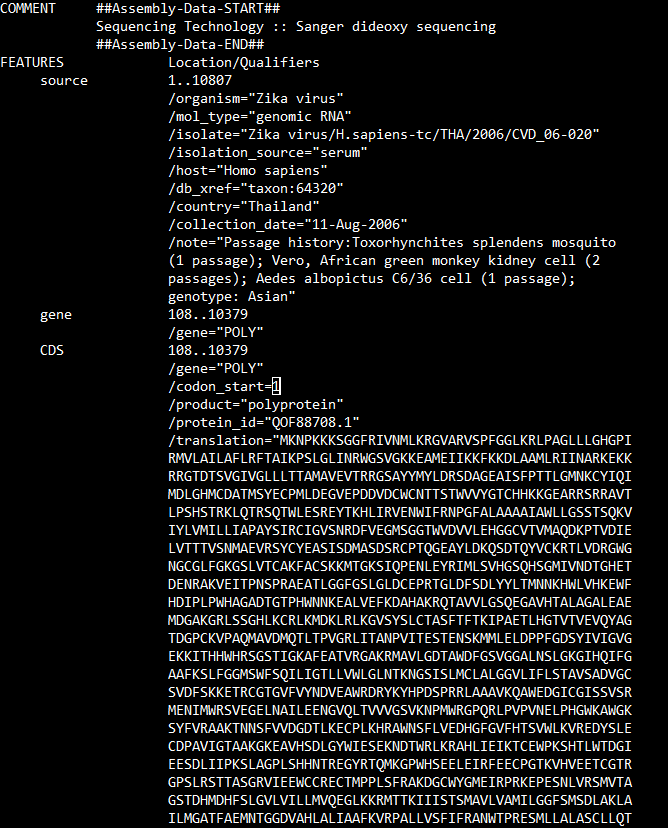
\includegraphics{images/zika-features.png}

}

\caption{alt text}

\end{figure}%

\begin{itemize}
\tightlist
\item
  Slicing
\end{itemize}

\begin{Shaded}
\begin{Highlighting}[]
\BuiltInTok{print}\NormalTok{(record.features[}\DecValTok{0}\NormalTok{])}
\BuiltInTok{print}\NormalTok{(record.features[}\DecValTok{1}\NormalTok{])}
\BuiltInTok{print}\NormalTok{(record.features[}\DecValTok{2}\NormalTok{])}
\end{Highlighting}
\end{Shaded}

\begin{verbatim}
type: source
location: [0:10807](+)
qualifiers:
    Key: collection_date, Value: ['11-Aug-2006']
    Key: country, Value: ['Thailand']
    Key: db_xref, Value: ['taxon:64320']
    Key: host, Value: ['Homo sapiens']
    Key: isolate, Value: ['Zika virus/H.sapiens-tc/THA/2006/CVD_06-020']
    Key: isolation_source, Value: ['serum']
    Key: mol_type, Value: ['genomic RNA']
    Key: note, Value: ['Passage history:Toxorhynchites splendens mosquito (1 passage); Vero, African green monkey kidney cell (2 passages); Aedes albopictus C6/36 cell (1 passage); genotype: Asian']
    Key: organism, Value: ['Zika virus']

type: gene
location: [107:10379](+)
qualifiers:
    Key: gene, Value: ['POLY']

type: CDS
location: [107:10379](+)
qualifiers:
    Key: codon_start, Value: ['1']
    Key: gene, Value: ['POLY']
    Key: product, Value: ['polyprotein']
    Key: protein_id, Value: ['QOF88708.1']
    Key: translation, Value: ['MKNPKKKSGGFRIVNMLKRGVARVSPFGGLKRLPAGLLLGHGPIRMVLAILAFLRFTAIKPSLGLINRWGSVGKKEAMEIIKKFKKDLAAMLRIINARKEKKRRGTDTSVGIVGLLLTTAMAVEVTRRGSAYYMYLDRSDAGEAISFPTTLGMNKCYIQIMDLGHMCDATMSYECPMLDEGVEPDDVDCWCNTTSTWVVYGTCHHKKGEARRSRRAVTLPSHSTRKLQTRSQTWLESREYTKHLIRVENWIFRNPGFALAAAAIAWLLGSSTSQKVIYLVMILLIAPAYSIRCIGVSNRDFVEGMSGGTWVDVVLEHGGCVTVMAQDKPTVDIELVTTTVSNMAEVRSYCYEASISDMASDSRCPTQGEAYLDKQSDTQYVCKRTLVDRGWGNGCGLFGKGSLVTCAKFACSKKMTGKSIQPENLEYRIMLSVHGSQHSGMIVNDTGHETDENRAKVEITPNSPRAEATLGGFGSLGLDCEPRTGLDFSDLYYLTMNNKHWLVHKEWFHDIPLPWHAGADTGTPHWNNKEALVEFKDAHAKRQTAVVLGSQEGAVHTALAGALEAEMDGAKGRLSSGHLKCRLKMDKLRLKGVSYSLCTASFTFTKIPAETLHGTVTVEVQYAGTDGPCKVPAQMAVDMQTLTPVGRLITANPVITESTENSKMMLELDPPFGDSYIVIGVGEKKITHHWHRSGSTIGKAFEATVRGAKRMAVLGDTAWDFGSVGGALNSLGKGIHQIFGAAFKSLFGGMSWFSQILIGTLLVWLGLNTKNGSISLMCLALGGVLIFLSTAVSADVGCSVDFSKKETRCGTGVFVYNDVEAWRDRYKYHPDSPRRLAAAVKQAWEDGICGISSVSRMENIMWRSVEGELNAILEENGVQLTVVVGSVKNPMWRGPQRLPVPVNELPHGWKAWGKSYFVRAAKTNNSFVVDGDTLKECPLKHRAWNSFLVEDHGFGVFHTSVWLKVREDYSLECDPAVIGTAAKGKEAVHSDLGYWIESEKNDTWRLKRAHLIEIKTCEWPKSHTLWTDGIEESDLIIPKSLAGPLSHHNTREGYRTQMKGPWHSEELEIRFEECPGTKVHVEETCGTRGPSLRSTTASGRVIEEWCCRECTMPPLSFRAKDGCWYGMEIRPRKEPESNLVRSMVTAGSTDHMDHFSLGVLVILLMVQEGLKKRMTTKIIISTSMAVLVAMILGGFSMSDLAKLAILMGATFAEMNTGGDVAHLALIAAFKVRPALLVSFIFRANWTPRESMLLALASCLLQTAISALEGDLMVLINGFALAWLAIRAMVVPRTDNITLAILAALTPLARGTLLVAWRAGLATCGGFMLLSLKGRGSVKKNLPFVMALGLTAVRLVDPINVVGLLLLTRSGKRSWPPSEVLTAVGLICALAGGFAKADIEMAGPIAAVGLLIVSYVVSGKSVDMYIERAGDITWEKDAEVTGNSPRLDVALDESGDFSLVEDDGPPMREIILKVVLMAICGMNPIAIPFAAGAWYVYVKTGKRSGALWDVPAPKEVKKGETTDGVYRVMTRRLLGSTQVGVGVMQEGVFHTMWHVTKGSALRSGEGRLDPYWGDVKQDLVSYCGPWKLDAAWDGHSEVQLLAVPPGERARNIQTLPGIFKTKDGDIGAVALDYPAGTSGSPILDKCGRVIGLYGNGVVIKNGSYVSAITQGRREEETPVECFEPSMLKKKQLTVLDLHPGAGKTRRVLPEIVREAIKTRLRTVILAPTRVVAAEMEEALRGLPVRYMTTAVNVTHSGTEIVDLMCHATFTSRLLQPIRVPNYNLYIMDEAHFTDPSSIAARGYISTRVEMGEAAAIFMTATPPGTRDAFPDSNSPIMDTEVEVPERAWSSGFDWVTDHSGKTVWFVPSVRNGNEIAACLTKAGKRVIQLSRKTFETEFQKTKHQEWDFVVTTDISEMGANFKADRVIDSRRCLKPVILDGERVILAGPMPVTHASAAQRRGRIGRNPNKPGDEYLYGGGCAETDEDHAHWLEARMLLDNIYLQDGLIASLYRPEADKVAAIEGEFKLRTEQRKTFVELMKRGDLPVWLAYQVASAGITYTDRRWCFDGTTNNTIMEDSVPAEVWTRYGEKRVLKPRWMDARVCSDHAALKSFKEFAAGKRGAAFGVMEALGTLPGHMTERFQEAIDNLAVLMRAETGSRPYKAAAAQLPETLETIMLLGLLGTVSLGIFFVLMRNKGIGKMGFGMVTLGASAWLMWLSEIEPARIACVLIVVFLLLVVLIPEPEKQRSPQDNQMAIIIMVAVGLLGLITANELGWLERTKSDLSHLMGRREEGATIGFSMDIDLRPASAWAIYAALTTFITPAVQHAVTTSYNNYSLMAMATQAGVLFGMGKGMPFYAWDFGVPLLMIGCYSQLTPLTLIVAIILLVAHYMYLIPGLQAAAARAAQKRTAAGIMKNPVVDGIVVTDIDTMTIDPQVEKKMGQVLLIAVAVSSAILSRTAWGWGEAGALITAATSTLWEGSPNKYWNSSTATSLCNIFRGSYLAGASLIYTVTRNAGLVKRRGGGTGETLGEKWKARLNQMSALEFYSYKKSGITEVCREEARRALKDGVATGGHAVSRGSAKLRWLVERGYLQPYGKVIDLGCGRGGWSYYAATIRKVQEVKGYTKGGPGHEEPMLVQSYGWNIVRLKSGVDVFHMAAEPCDTLLCDIGESSSSPEVEEARTLRVLSMVGDWLEKRPGAFCIKVLCPYTSTMMETLERLQRRYGGGLVRVPLSRNSTHEMYWVSGAKSNTIKSVSTTSQLLLGRMDGPRRPVKYEEDVNLGSGTRAVVSCAEAPNMKIIGNRIERIRSEHAETWFFDENHPYRTWAYHGSYEAPTQGSASSLINGVVRLLSKPWDVVTGVTGIAMTDTTPYGQQRVFKEKVDTRVPDPQEGTRQVMSMVSSWLWKELGKHKRPRVCTKEEFINKVRSNAALGAIFEEEKEWKTAVEAVNDPRFWALVDKEREHHLRGECQSCVYNMMGKREKKQGEFGKAKGSRAIWYMWLGARFLEFEALGFLNEDHWMGRENSRGGVEGLGLQRLGYVLEEMSRIPGGRMYADDTAGWDTRISRFDLENEALITNQMEKGHRALALAIIKYTYQNKVVKVLRPAEKGKTVMDIISRQDQRGSGQVVTYALNTFTNLVVQLIRNMEAEEVLEMQDLWLLRRSEKVTNWLQSNGWDRLKRMAVSGDDCVVKPIDDRFAHALRFLNDMGKVRKDTQEWKPSTGWDNWEEVPFCSHHFNKLHLKDGRSIVVPCRHQDELIGRARVSPGAGWSIRETACLAKSYAQMWQLLYFHRRDLRLMANAICSSVPVDWVPTGRTTWSIHGKGEWMTTEDMLVVWNRVWIEENDHMEDKTPVTKWTDIPYLGKREDLWCGSLIGHRPRTTWAENIKNTVNMMRRIIGDEEKYMDYLSTQVRYLGEEGSTPGVL']
\end{verbatim}

\begin{itemize}
\tightlist
\item
  extract sequence
\end{itemize}

\begin{Shaded}
\begin{Highlighting}[]
\NormalTok{record.features[}\DecValTok{2}\NormalTok{].extract(record.seq)}
\end{Highlighting}
\end{Shaded}

\begin{verbatim}
Seq('ATGAAAAACCCAAAGAAGAAATCCGGAGGATTCCGGATTGTCAATATGCTAAAA...TAA')
\end{verbatim}

\begin{itemize}
\tightlist
\item
  위치 탐색 in 활용
\end{itemize}

\begin{Shaded}
\begin{Highlighting}[]
\ControlFlowTok{for}\NormalTok{ feature }\KeywordTok{in}\NormalTok{ record.features:}
    \ControlFlowTok{if} \DecValTok{4350} \KeywordTok{in}\NormalTok{ feature:}
        \BuiltInTok{print}\NormalTok{(}\SpecialStringTok{f"type: }\SpecialCharTok{\{}\NormalTok{feature}\SpecialCharTok{.}\BuiltInTok{type}\SpecialCharTok{\}}\SpecialStringTok{ start: }\SpecialCharTok{\{}\NormalTok{feature}\SpecialCharTok{.}\NormalTok{location}\SpecialCharTok{.}\NormalTok{start}\SpecialCharTok{\}}\SpecialStringTok{ end: }\SpecialCharTok{\{}\NormalTok{feature}\SpecialCharTok{.}\NormalTok{location}\SpecialCharTok{.}\NormalTok{end}\SpecialCharTok{\}}\SpecialStringTok{"}\NormalTok{)}
\end{Highlighting}
\end{Shaded}

\begin{verbatim}
type: source start: 0 end: 10807
type: gene start: 107 end: 10379
type: CDS start: 107 end: 10379
type: mat_peptide start: 4223 end: 4613
\end{verbatim}

\begin{itemize}
\tightlist
\item
  서열 위치로 직접 슬라이싱
\end{itemize}

\begin{Shaded}
\begin{Highlighting}[]
\NormalTok{sub\_record }\OperatorTok{=}\NormalTok{ record[}\DecValTok{3000}\NormalTok{:}\DecValTok{5000}\NormalTok{]}
\BuiltInTok{print}\NormalTok{(sub\_record)}
\BuiltInTok{print}\NormalTok{(}\BuiltInTok{len}\NormalTok{(sub\_record))}
\BuiltInTok{print}\NormalTok{(}\BuiltInTok{len}\NormalTok{(sub\_record.features))}
\BuiltInTok{print}\NormalTok{(sub\_record.features[}\DecValTok{0}\NormalTok{])}
\BuiltInTok{print}\NormalTok{(sub\_record.features[}\DecValTok{1}\NormalTok{])}
\end{Highlighting}
\end{Shaded}

\begin{verbatim}
ID: MW015936.1
Name: MW015936
Description: Zika virus isolate Zika virus/H.sapiens-tc/THA/2006/CVD_06-020, complete genome
Number of features: 2
/molecule_type=RNA
Seq('TTAGAGAAGATTATTCATTAGAGTGTGATCCAGCCGTCATTGGAACAGCCGCTA...GAC')
2000
2
type: mat_peptide
location: [545:1223](+)
qualifiers:
    Key: gene, Value: ['POLY']
    Key: product, Value: ['nonstructural protein NS2A']

type: mat_peptide
location: [1223:1613](+)
qualifiers:
    Key: gene, Value: ['POLY']
    Key: product, Value: ['nonstructural protein NS2B']
\end{verbatim}

\subsubsection{Example - find features and
plot}\label{example---find-features-and-plot}

{[}User{]}

{ I have a genbank file. I want extract all the features of
``mat\_peptide'' type in the file and calculate their length. can you
show me a python code? }

{[}ChatGPT{]}

Certainly! You can use Biopython to read a GenBank file and extract
features of a specific type, such as ``mat\_peptide''. Here's how you
can do it:

\textbf{Python Script}

Here is the Python script that extracts all ``mat\_peptide'' features
from a GenBank file and calculates their lengths:

\begin{Shaded}
\begin{Highlighting}[]
\ImportTok{from}\NormalTok{ Bio }\ImportTok{import}\NormalTok{ SeqIO}

\CommentTok{\# Function to extract mat\_peptide features and calculate their lengths}
\KeywordTok{def}\NormalTok{ extract\_mat\_peptide\_features(file\_path):}
\NormalTok{    record }\OperatorTok{=}\NormalTok{ SeqIO.read(file\_path, }\StringTok{"genbank"}\NormalTok{)}
\NormalTok{    mat\_peptides }\OperatorTok{=}\NormalTok{ []}

    \ControlFlowTok{for}\NormalTok{ feature }\KeywordTok{in}\NormalTok{ record.features:}
        \ControlFlowTok{if}\NormalTok{ feature.}\BuiltInTok{type} \OperatorTok{==} \StringTok{"mat\_peptide"}\NormalTok{:}
\NormalTok{            start }\OperatorTok{=}\NormalTok{ feature.location.start.position}
\NormalTok{            end }\OperatorTok{=}\NormalTok{ feature.location.end.position}
\NormalTok{            length }\OperatorTok{=}\NormalTok{ end }\OperatorTok{{-}}\NormalTok{ start}
\NormalTok{            mat\_peptides.append(\{}
                \StringTok{"ID"}\NormalTok{: feature.qualifiers.get(}\StringTok{"product"}\NormalTok{, [}\StringTok{"Unknown"}\NormalTok{])[}\DecValTok{0}\NormalTok{],}
                \StringTok{"Start"}\NormalTok{: start,}
                \StringTok{"End"}\NormalTok{: end,}
                \StringTok{"Length"}\NormalTok{: length}
\NormalTok{            \})}
    
    \ControlFlowTok{return}\NormalTok{ mat\_peptides}

\CommentTok{\# Example usage}
\NormalTok{genbank\_file }\OperatorTok{=} \StringTok{\textquotesingle{}example.gb\textquotesingle{}}  \CommentTok{\# Replace with your GenBank file path}
\NormalTok{mat\_peptide\_features }\OperatorTok{=}\NormalTok{ extract\_mat\_peptide\_features(genbank\_file)}

\CommentTok{\# Print the results}
\ControlFlowTok{for}\NormalTok{ peptide }\KeywordTok{in}\NormalTok{ mat\_peptide\_features:}
    \BuiltInTok{print}\NormalTok{(}\SpecialStringTok{f"ID: }\SpecialCharTok{\{}\NormalTok{peptide[}\StringTok{\textquotesingle{}ID\textquotesingle{}}\NormalTok{]}\SpecialCharTok{\}}\SpecialStringTok{, Start: }\SpecialCharTok{\{}\NormalTok{peptide[}\StringTok{\textquotesingle{}Start\textquotesingle{}}\NormalTok{]}\SpecialCharTok{\}}\SpecialStringTok{, End: }\SpecialCharTok{\{}\NormalTok{peptide[}\StringTok{\textquotesingle{}End\textquotesingle{}}\NormalTok{]}\SpecialCharTok{\}}\SpecialStringTok{, Length: }\SpecialCharTok{\{}\NormalTok{peptide[}\StringTok{\textquotesingle{}Length\textquotesingle{}}\NormalTok{]}\SpecialCharTok{\}}\SpecialStringTok{ bp"}\NormalTok{)}
\end{Highlighting}
\end{Shaded}

\textbf{Explanation}

\begin{enumerate}
\def\labelenumi{\arabic{enumi}.}
\tightlist
\item
  \textbf{Import Libraries}: Import the necessary modules from
  Biopython.
\item
  \textbf{extract\_mat\_peptide\_features Function}: This function reads
  the GenBank file, extracts features of type ``mat\_peptide'',
  calculates their start and end positions, and determines their
  lengths.
\item
  \textbf{Example Usage}: Replace
  \texttt{\textquotesingle{}example.gb\textquotesingle{}} with the path
  to your GenBank file. The script will read the file, extract the
  ``mat\_peptide'' features, and print their IDs, start and end
  positions, and lengths.
\end{enumerate}

\textbf{Running the Script}

\begin{enumerate}
\def\labelenumi{\arabic{enumi}.}
\item
  Save the script to a file, for example,
  \texttt{extract\_mat\_peptides.py}.
\item
  Ensure you have the GenBank file (e.g., \texttt{example.gb}) in the
  same directory.
\item
  Run the script from the command line:

\begin{Shaded}
\begin{Highlighting}[]
\ExtensionTok{python}\NormalTok{ extract\_mat\_peptides.py}
\end{Highlighting}
\end{Shaded}
\end{enumerate}

This script will read the GenBank file, extract all ``mat\_peptide''
features, calculate their lengths, and print the details. If you have
any specific questions or need further assistance, feel free to ask!

\begin{itemize}
\tightlist
\item
  Find a specific feature
\end{itemize}

\begin{Shaded}
\begin{Highlighting}[]
\ImportTok{from}\NormalTok{ Bio }\ImportTok{import}\NormalTok{ SeqIO}

\NormalTok{records }\OperatorTok{=}\NormalTok{ SeqIO.parse(}\StringTok{"data/MW015936.gb"}\NormalTok{, }\StringTok{"genbank"}\NormalTok{)}
\ControlFlowTok{for}\NormalTok{ feature }\KeywordTok{in}\NormalTok{ record.features:}
    \ControlFlowTok{if}\NormalTok{ feature.}\BuiltInTok{type} \OperatorTok{==} \StringTok{"mat\_peptide"}\NormalTok{:}
        \BuiltInTok{print}\NormalTok{(feature.qualifiers[}\StringTok{"product"}\NormalTok{])}
        \BuiltInTok{print}\NormalTok{(feature.location.start, feature.location.end)}
\end{Highlighting}
\end{Shaded}

\begin{verbatim}
['anchored capsid protein C']
107 473
['capsid protein C']
107 419
['membrane glycoprotein precursor M']
473 977
['protein pr']
473 752
['membrane glycoprotein M']
752 977
['envelope protein E']
977 2489
['nonstructural protein NS1']
2489 3545
['nonstructural protein NS2A']
3545 4223
['nonstructural protein NS2B']
4223 4613
['nonstructural protein NS3']
4613 6464
['nonstructural protein NS4A']
6464 6845
['protein 2K']
6845 6914
['nonstructural protein NS4B']
6914 7667
['RNA-dependent RNA polymerase NS5']
7667 10376
\end{verbatim}

\begin{itemize}
\tightlist
\item
  get length and plot
\end{itemize}

\begin{Shaded}
\begin{Highlighting}[]
\ImportTok{from}\NormalTok{ Bio }\ImportTok{import}\NormalTok{ SeqIO}
\ImportTok{import}\NormalTok{ pandas }\ImportTok{as}\NormalTok{ pd}
\ImportTok{from}\NormalTok{ matplotlib }\ImportTok{import}\NormalTok{ pyplot }\ImportTok{as}\NormalTok{ plt}
\ImportTok{import}\NormalTok{ seaborn }\ImportTok{as}\NormalTok{ sns}

\NormalTok{mat\_peptides }\OperatorTok{=}\NormalTok{ []}
\NormalTok{records }\OperatorTok{=}\NormalTok{ SeqIO.parse(}\StringTok{"data/MW015936.gb"}\NormalTok{, }\StringTok{"genbank"}\NormalTok{)}
\ControlFlowTok{for}\NormalTok{ feature }\KeywordTok{in}\NormalTok{ record.features:}
    \ControlFlowTok{if}\NormalTok{ feature.}\BuiltInTok{type} \OperatorTok{==} \StringTok{"mat\_peptide"}\NormalTok{:}
\NormalTok{        mat\_peptides.append(\{}
            \StringTok{"id"}\NormalTok{: feature.qualifiers[}\StringTok{"product"}\NormalTok{],}
            \StringTok{"start"}\NormalTok{: feature.location.start,}
            \StringTok{"end"}\NormalTok{: feature.location.end,}
            \StringTok{"length"}\NormalTok{: feature.location.end }\OperatorTok{{-}}\NormalTok{ feature.location.start}
\NormalTok{        \})}

\NormalTok{df }\OperatorTok{=}\NormalTok{ pd.DataFrame(mat\_peptides)}

\NormalTok{plt.figure(figsize }\OperatorTok{=}\NormalTok{ (}\DecValTok{10}\NormalTok{, }\DecValTok{6}\NormalTok{))}
\CommentTok{\# df["length"].hist()}
\NormalTok{sns.histplot(df[}\StringTok{"length"}\NormalTok{])}
\NormalTok{plt.xticks(rotation }\OperatorTok{=} \DecValTok{90}\NormalTok{)}
\NormalTok{plt.show()}
\end{Highlighting}
\end{Shaded}

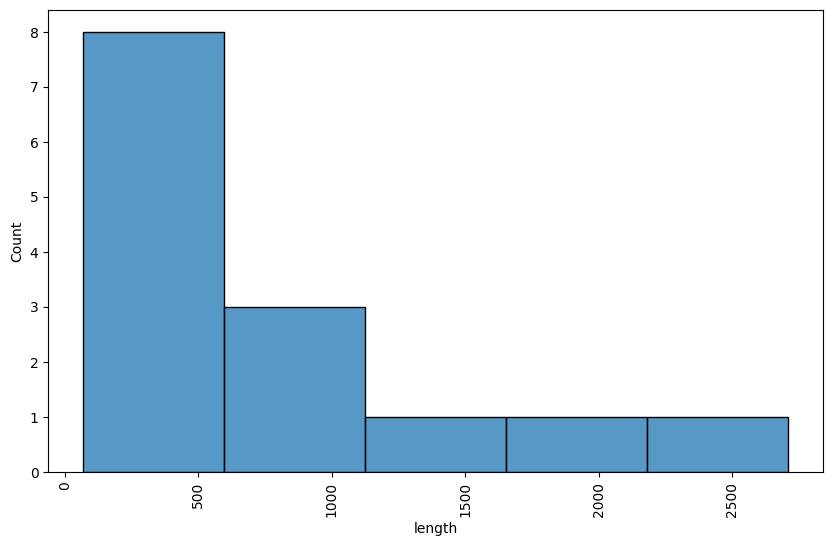
\includegraphics{cnu_bioinformatics_files/figure-pdf/cell-26-output-1.png}

\subsection{Entrez}\label{entrez}

\begin{itemize}
\tightlist
\item
  Provides code to access NCBI over the WWW
\item
  파일 읽기/쓰기 with 문 사용
\end{itemize}

\begin{Shaded}
\begin{Highlighting}[]
\ImportTok{from}\NormalTok{ Bio }\ImportTok{import}\NormalTok{ Entrez}
\NormalTok{Entrez.email }\OperatorTok{=} \StringTok{"kimhaseong@gmail.com"}

\CommentTok{\# Searching NCBI Nucleotide database}
\NormalTok{handle }\OperatorTok{=}\NormalTok{ Entrez.esearch(db}\OperatorTok{=}\StringTok{"nucleotide"}\NormalTok{, term}\OperatorTok{=}\StringTok{"Homo sapiens[Organism] AND BRCA1[Gene]"}\NormalTok{, retmax}\OperatorTok{=}\DecValTok{5}\NormalTok{)}
\NormalTok{record }\OperatorTok{=}\NormalTok{ Entrez.read(handle)}
\BuiltInTok{print}\NormalTok{(record[}\StringTok{"IdList"}\NormalTok{])}
\end{Highlighting}
\end{Shaded}

\begin{verbatim}
['262359905', '2703623457', '2703623455', '2703623453', '2703623451']
\end{verbatim}

\begin{Shaded}
\begin{Highlighting}[]
\ImportTok{from}\NormalTok{ Bio }\ImportTok{import}\NormalTok{ Entrez}
\ImportTok{from}\NormalTok{ Bio }\ImportTok{import}\NormalTok{ SeqIO}
\NormalTok{entid }\OperatorTok{=}\NormalTok{ record[}\StringTok{"IdList"}\NormalTok{][}\DecValTok{0}\NormalTok{]}

\ControlFlowTok{with}\NormalTok{ Entrez.efetch(db}\OperatorTok{=}\StringTok{"nucleotide"}\NormalTok{, rettype}\OperatorTok{=}\StringTok{"gb"}\NormalTok{, retmode}\OperatorTok{=}\StringTok{"text"}\NormalTok{, }\BuiltInTok{id}\OperatorTok{=}\NormalTok{entid) }\ImportTok{as}\NormalTok{ handle:}
\NormalTok{    seq\_record }\OperatorTok{=}\NormalTok{ SeqIO.read(handle, }\StringTok{"gb"}\NormalTok{)}
\BuiltInTok{print}\NormalTok{(}\SpecialStringTok{f"}\SpecialCharTok{\{}\NormalTok{seq\_record}\SpecialCharTok{.}\BuiltInTok{id}\SpecialCharTok{\}}\SpecialStringTok{ with }\SpecialCharTok{\{}\BuiltInTok{len}\NormalTok{(seq\_record.features)}\SpecialCharTok{\}}\SpecialStringTok{ features"}\NormalTok{)}
\BuiltInTok{print}\NormalTok{(}\BuiltInTok{type}\NormalTok{(seq\_record))}
\NormalTok{SeqIO.write(seq\_record, }\StringTok{"/content/drive/My Drive/2024{-}cnu{-}lecture/data/"}\OperatorTok{+}\NormalTok{seq\_record.}\BuiltInTok{id}\OperatorTok{+}\StringTok{".fa"}\NormalTok{, }\StringTok{"fasta"}\NormalTok{)}
\CommentTok{\#SeqIO.write(seq\_record, seq\_record.id+".fa", "fasta")}
\BuiltInTok{print}\NormalTok{(seq\_record)}
\end{Highlighting}
\end{Shaded}

\begin{verbatim}
NG_005905.2 with 130 features
<class 'Bio.SeqRecord.SeqRecord'>
ID: NG_005905.2
Name: NG_005905
Description: Homo sapiens BRCA1 DNA repair associated (BRCA1), RefSeqGene (LRG_292) on chromosome 17
Number of features: 130
/molecule_type=DNA
/topology=linear
/data_file_division=PRI
/date=09-JUN-2024
/accessions=['NG_005905']
/sequence_version=2
/keywords=['RefSeq', 'RefSeqGene']
/source=Homo sapiens (human)
/organism=Homo sapiens
/taxonomy=['Eukaryota', 'Metazoa', 'Chordata', 'Craniata', 'Vertebrata', 'Euteleostomi', 'Mammalia', 'Eutheria', 'Euarchontoglires', 'Primates', 'Haplorrhini', 'Catarrhini', 'Hominidae', 'Homo']
/references=[Reference(title='Emerging roles of BRCA1 alternative splicing', ...), Reference(title='Expression profiles of BRCA1 splice variants in asynchronous and in G1/S synchronized tumor cell lines', ...), Reference(title='BRCA1: a review of structure and putative functions', ...), Reference(title='Mutations and alternative splicing of the BRCA1 gene in UK breast/ovarian cancer families', ...), Reference(title='Differential subcellular localization, expression and biological toxicity of BRCA1 and the splice variant BRCA1-delta11b', ...), Reference(title='Localization of BRCA1 and a splice variant identifies the nuclear localization signal', ...), Reference(title='Characterization of functional messenger RNA splice variants of BRCA1 expressed in nonmalignant and tumor-derived breast cells', ...), Reference(title='Growth retardation and tumour inhibition by BRCA1', ...), Reference(title='Distinct transcription start sites generate two forms of BRCA1 mRNA', ...), Reference(title='A strong candidate for the breast and ovarian cancer susceptibility gene BRCA1', ...), Reference(title='Fanconi Anemia', ...), Reference(title='BRCA1- and BRCA2-Associated Hereditary Breast and Ovarian Cancer', ...)]
/comment=REVIEWED REFSEQ: This record has been curated by NCBI staff in
collaboration with Andrew Devereau, Nazneen Rahman. The reference
sequence was derived from AC109326.11, AC060780.18 and AC135721.4.
This sequence is a reference standard in the RefSeqGene project.
On Nov 4, 2009 this sequence version replaced NG_005905.1.
Summary: This gene encodes a 190 kD nuclear phosphoprotein that
plays a role in maintaining genomic stability, and it also acts as
a tumor suppressor. The BRCA1 gene contains 22 exons spanning about
110 kb of DNA. The encoded protein combines with other tumor
suppressors, DNA damage sensors, and signal transducers to form a
large multi-subunit protein complex known as the BRCA1-associated
genome surveillance complex (BASC). This gene product associates
with RNA polymerase II, and through the C-terminal domain, also
interacts with histone deacetylase complexes. This protein thus
plays a role in transcription, DNA repair of double-stranded
breaks, and recombination. Mutations in this gene are responsible
for approximately 40% of inherited breast cancers and more than 80%
of inherited breast and ovarian cancers. Alternative splicing plays
a role in modulating the subcellular localization and physiological
function of this gene. Many alternatively spliced transcript
variants, some of which are disease-associated mutations, have been
described for this gene, but the full-length natures of only some
of these variants has been described. A related pseudogene, which
is also located on chromosome 17, has been identified. [provided by
RefSeq, May 2020].
Seq('TGTGTGTATGAAGTTAACTTCAAAGCAAGCTTCCTGTGCTGAGGGGGTGGGAGG...GGC')
\end{verbatim}

\begin{itemize}
\tightlist
\item
  여러개 record에 대해서는 parse 함수를 사용
\end{itemize}

\begin{Shaded}
\begin{Highlighting}[]
\ImportTok{from}\NormalTok{ Bio }\ImportTok{import}\NormalTok{ SeqIO}

\NormalTok{entids }\OperatorTok{=}\NormalTok{ record[}\StringTok{"IdList"}\NormalTok{]}

\ControlFlowTok{with}\NormalTok{ Entrez.efetch(db}\OperatorTok{=}\StringTok{"nucleotide"}\NormalTok{, rettype}\OperatorTok{=}\StringTok{"gb"}\NormalTok{, retmode}\OperatorTok{=}\StringTok{"text"}\NormalTok{, }\BuiltInTok{id}\OperatorTok{=}\NormalTok{entids) }\ImportTok{as}\NormalTok{ handle:}
    \ControlFlowTok{for}\NormalTok{ seq\_record }\KeywordTok{in}\NormalTok{ SeqIO.parse(handle, }\StringTok{"gb"}\NormalTok{):}
        \BuiltInTok{print}\NormalTok{(}\SpecialStringTok{f"}\SpecialCharTok{\{}\NormalTok{seq\_record}\SpecialCharTok{.}\BuiltInTok{id}\SpecialCharTok{\}}\SpecialStringTok{ }\SpecialCharTok{\{}\NormalTok{seq\_record}\SpecialCharTok{.}\NormalTok{description[:}\DecValTok{50}\NormalTok{]}\SpecialCharTok{\}}\SpecialStringTok{"}\NormalTok{)}
        \BuiltInTok{print}\NormalTok{(}\SpecialStringTok{f"Sequence length }\SpecialCharTok{\{}\BuiltInTok{len}\NormalTok{(seq\_record)}\SpecialCharTok{\}}\SpecialStringTok{, }\SpecialCharTok{\{}\BuiltInTok{len}\NormalTok{(seq\_record.features)}\SpecialCharTok{\}}\SpecialStringTok{ }\CharTok{\textbackslash{}}
\SpecialStringTok{              features, from }\SpecialCharTok{\{}\NormalTok{seq\_record}\SpecialCharTok{.}\NormalTok{annotations[}\StringTok{\textquotesingle{}source\textquotesingle{}}\NormalTok{]}\SpecialCharTok{\}}\SpecialStringTok{"}\NormalTok{)}
        \BuiltInTok{print}\NormalTok{(}\StringTok{"}\CharTok{\textbackslash{}n}\StringTok{"}\NormalTok{)}
\NormalTok{        SeqIO.write(seq\_record, }\StringTok{"/content/drive/My Drive/2024{-}cnu{-}lecture/data/"}\OperatorTok{+}\NormalTok{seq\_record.}\BuiltInTok{id}\OperatorTok{+}\StringTok{".gb"}\NormalTok{, }\StringTok{"gb"}\NormalTok{)}
\end{Highlighting}
\end{Shaded}

\begin{verbatim}
NG_005905.2 Homo sapiens BRCA1 DNA repair associated (BRCA1), 
Sequence length 193689, 130               features, from Homo sapiens (human)


PP465840.1 Homo sapiens isolate TWH-3503-0-1 breast and ovari
Sequence length 5592, 3               features, from Homo sapiens (human)


PP465839.1 Homo sapiens isolate TWH-3747-0-1 truncated breast
Sequence length 891, 3               features, from Homo sapiens (human)


PP465838.1 Homo sapiens isolate TWH-3713-0-1 truncated breast
Sequence length 3462, 3               features, from Homo sapiens (human)


PP465837.1 Homo sapiens isolate OV-0673-0-1 truncated breast 
Sequence length 4167, 3               features, from Homo sapiens (human)

\end{verbatim}

\subsection{Pairwise sequence
alignment}\label{pairwise-sequence-alignment}

\begin{Shaded}
\begin{Highlighting}[]
\ImportTok{from}\NormalTok{ Bio }\ImportTok{import}\NormalTok{ Align}

\NormalTok{aligner }\OperatorTok{=}\NormalTok{ Align.PairwiseAligner()}
\NormalTok{aligner.mode }\OperatorTok{=} \StringTok{"global"}
\NormalTok{aligner.mismatch\_score }\OperatorTok{=} \OperatorTok{{-}}\DecValTok{10}
\NormalTok{alignments }\OperatorTok{=}\NormalTok{ aligner.align(}\StringTok{"AAACAAA"}\NormalTok{, }\StringTok{"ACGAAAGAAA"}\NormalTok{)}
\BuiltInTok{print}\NormalTok{(aligner)}
\BuiltInTok{print}\NormalTok{(}\BuiltInTok{len}\NormalTok{(alignments))}
\BuiltInTok{print}\NormalTok{(alignments.score)}

\BuiltInTok{print}\NormalTok{(alignments[}\DecValTok{0}\NormalTok{])}
\BuiltInTok{print}\NormalTok{(alignments[}\DecValTok{1}\NormalTok{])}
\BuiltInTok{print}\NormalTok{(alignments[}\DecValTok{2}\NormalTok{])}
\end{Highlighting}
\end{Shaded}

\begin{verbatim}
Pairwise sequence aligner with parameters
  wildcard: None
  match_score: 1.000000
  mismatch_score: -10.000000
  target_internal_open_gap_score: 0.000000
  target_internal_extend_gap_score: 0.000000
  target_left_open_gap_score: 0.000000
  target_left_extend_gap_score: 0.000000
  target_right_open_gap_score: 0.000000
  target_right_extend_gap_score: 0.000000
  query_internal_open_gap_score: 0.000000
  query_internal_extend_gap_score: 0.000000
  query_left_open_gap_score: 0.000000
  query_left_extend_gap_score: 0.000000
  query_right_open_gap_score: 0.000000
  query_right_extend_gap_score: 0.000000
  mode: global

12
6.0
target            0 A--AACA-AA-  7
                  0 |--||-|-||- 11
query             0 ACGAA-AGAAA 10

target            0 A--AACA-A-A  7
                  0 |--||-|-|-| 11
query             0 ACGAA-AGAAA 10

target            0 A--AACA--AA  7
                  0 |--||-|--|| 11
query             0 ACGAA-AGAAA 10
\end{verbatim}

\begin{Shaded}
\begin{Highlighting}[]
\NormalTok{aligner }\OperatorTok{=}\NormalTok{ Align.PairwiseAligner(mismatch\_score}\OperatorTok{={-}}\DecValTok{10}\NormalTok{, mode}\OperatorTok{=}\StringTok{"local"}\NormalTok{)}
\NormalTok{alignments }\OperatorTok{=}\NormalTok{ aligner.align(}\StringTok{"AAACAAA"}\NormalTok{, }\StringTok{"ACGAAAGAAA"}\NormalTok{)}
\BuiltInTok{print}\NormalTok{(}\BuiltInTok{len}\NormalTok{(alignments))}
\BuiltInTok{print}\NormalTok{(alignments.score)}

\BuiltInTok{print}\NormalTok{(alignments[}\DecValTok{0}\NormalTok{])}
\BuiltInTok{print}\NormalTok{(alignments[}\DecValTok{1}\NormalTok{])}
\BuiltInTok{print}\NormalTok{(alignments[}\DecValTok{2}\NormalTok{])}
\end{Highlighting}
\end{Shaded}

\begin{verbatim}
12
6.0
target            0 A--AACA-AA  7
                  0 |--||-|-|| 10
query             0 ACGAA-AGAA  9

target            0 A--AACA-A-A  7
                  0 |--||-|-|-| 11
query             0 ACGAA-AGAAA 10

target            0 A--AACA--AA  7
                  0 |--||-|--|| 11
query             0 ACGAA-AGAAA 10
\end{verbatim}

\subsubsection{Alignment objects}\label{alignment-objects}

\begin{Shaded}
\begin{Highlighting}[]

\BuiltInTok{print}\NormalTok{(alignments[}\DecValTok{0}\NormalTok{])}
\BuiltInTok{print}\NormalTok{(}\BuiltInTok{type}\NormalTok{(alignments[}\DecValTok{0}\NormalTok{]))}
\BuiltInTok{print}\NormalTok{(alignments[}\DecValTok{0}\NormalTok{].shape)}
\BuiltInTok{print}\NormalTok{(alignments[}\DecValTok{0}\NormalTok{].indices)}

\BuiltInTok{print}\NormalTok{(alignments[}\DecValTok{0}\NormalTok{].counts())}
\NormalTok{display(alignments[}\DecValTok{0}\NormalTok{].frequencies)}
\end{Highlighting}
\end{Shaded}

\begin{verbatim}
target            0 A--AACA-AA  7
                  0 |--||-|-|| 10
query             0 ACGAA-AGAA  9

<class 'Bio.Align.Alignment'>
(2, 10)
[[ 0 -1 -1  1  2  3  4 -1  5  6]
 [ 0  1  2  3  4 -1  5  6  7  8]]
AlignmentCounts(gaps=4, identities=6, mismatches=0)
\end{verbatim}

\begin{verbatim}
{'A': array([2., 0., 0., 2., 2., 0., 2., 0., 2., 2.]),
 '-': array([0., 1., 1., 0., 0., 1., 0., 1., 0., 0.]),
 'C': array([0., 1., 0., 0., 0., 1., 0., 0., 0., 0.]),
 'G': array([0., 0., 1., 0., 0., 0., 0., 1., 0., 0.])}
\end{verbatim}

\subsubsection{{[}User{]} biopython을 사용해서 NCBI에서 egfp 와 sfgfp
서열을 다운로드 받고 서열을 비교하는 코드를
알려줘}\label{user-biopythonuxc744-uxc0acuxc6a9uxd574uxc11c-ncbiuxc5d0uxc11c-egfp-uxc640-sfgfp-uxc11cuxc5f4uxc744-uxb2e4uxc6b4uxb85cuxb4dc-uxbc1buxace0-uxc11cuxc5f4uxc744-uxbe44uxad50uxd558uxb294-uxcf54uxb4dcuxb97c-uxc54cuxb824uxc918}

\subsubsection{{[}ChatGPT{]}}\label{chatgpt-9}

\begin{Shaded}
\begin{Highlighting}[]
\ImportTok{from}\NormalTok{ Bio }\ImportTok{import}\NormalTok{ Entrez, SeqIO}
\ImportTok{from}\NormalTok{ Bio.Seq }\ImportTok{import}\NormalTok{ Seq}
\ImportTok{from}\NormalTok{ Bio.SeqRecord }\ImportTok{import}\NormalTok{ SeqRecord}
\ImportTok{from}\NormalTok{ Bio }\ImportTok{import}\NormalTok{ pairwise2}
\ImportTok{from}\NormalTok{ Bio.pairwise2 }\ImportTok{import}\NormalTok{ format\_alignment}

\CommentTok{\# Always provide your email when using NCBI\textquotesingle{}s Entrez}
\NormalTok{Entrez.email }\OperatorTok{=} \StringTok{"your.email@example.com"}  \CommentTok{\# Replace with your email address}

\KeywordTok{def}\NormalTok{ download\_sequence(accession):}
    \CommentTok{"""Download a sequence by its accession number from NCBI."""}
\NormalTok{    handle }\OperatorTok{=}\NormalTok{ Entrez.efetch(db}\OperatorTok{=}\StringTok{"nucleotide"}\NormalTok{, }\BuiltInTok{id}\OperatorTok{=}\NormalTok{accession, rettype}\OperatorTok{=}\StringTok{"gb"}\NormalTok{, retmode}\OperatorTok{=}\StringTok{"text"}\NormalTok{)}
\NormalTok{    seq\_record }\OperatorTok{=}\NormalTok{ SeqIO.read(handle, }\StringTok{"genbank"}\NormalTok{)}
\NormalTok{    handle.close()}
    \ControlFlowTok{return}\NormalTok{ seq\_record}

\KeywordTok{def}\NormalTok{ compare\_sequences(seq1, seq2):}
    \CommentTok{"""Perform a simple sequence alignment between two sequences."""}
\NormalTok{    alignments }\OperatorTok{=}\NormalTok{ pairwise2.align.globalxx(seq1.seq, seq2.seq)}
    \ControlFlowTok{return}\NormalTok{ alignments[}\DecValTok{0}\NormalTok{]  }\CommentTok{\# Return the first alignment}

\CommentTok{\# Accession numbers for EGFP and sfGFP from NCBI}
\NormalTok{egfp\_accession }\OperatorTok{=} \StringTok{"U55762"}  \CommentTok{\# Example accession, update as necessary}
\NormalTok{sfgfp\_accession }\OperatorTok{=} \StringTok{"EU304438"}  \CommentTok{\# Example accession, update as necessary}

\CommentTok{\# Download sequences}
\NormalTok{egfp\_seq }\OperatorTok{=}\NormalTok{ download\_sequence(egfp\_accession)}
\NormalTok{sfgfp\_seq }\OperatorTok{=}\NormalTok{ download\_sequence(sfgfp\_accession)}

\CommentTok{\# Compare sequences}
\NormalTok{alignment }\OperatorTok{=}\NormalTok{ compare\_sequences(egfp\_seq, sfgfp\_seq)}

\CommentTok{\# Print alignment}
\BuiltInTok{print}\NormalTok{(format\_alignment(}\OperatorTok{*}\NormalTok{alignment))}
\end{Highlighting}
\end{Shaded}

\subsubsection{{[}User{]} 출력을 좀 더 보기 좋게
해줘}\label{user-uxcd9cuxb825uxc744-uxc880-uxb354-uxbcf4uxae30-uxc88buxac8c-uxd574uxc918}

\subsubsection{{[}ChatGTP{]}}\label{chatgtp}

\begin{Shaded}
\begin{Highlighting}[]
\ImportTok{from}\NormalTok{ Bio }\ImportTok{import}\NormalTok{ Entrez, SeqIO}
\ImportTok{from}\NormalTok{ Bio }\ImportTok{import}\NormalTok{ pairwise2}
\ImportTok{from}\NormalTok{ Bio.pairwise2 }\ImportTok{import}\NormalTok{ format\_alignment}

\CommentTok{\# Always provide your email when using NCBI\textquotesingle{}s Entrez}
\NormalTok{Entrez.email }\OperatorTok{=} \StringTok{"your.email@example.com"}  \CommentTok{\# Replace with your email address}

\KeywordTok{def}\NormalTok{ download\_sequence(accession):}
    \CommentTok{"""Download a sequence by its accession number from NCBI."""}
\NormalTok{    handle }\OperatorTok{=}\NormalTok{ Entrez.efetch(db}\OperatorTok{=}\StringTok{"nucleotide"}\NormalTok{, }\BuiltInTok{id}\OperatorTok{=}\NormalTok{accession, rettype}\OperatorTok{=}\StringTok{"gb"}\NormalTok{, retmode}\OperatorTok{=}\StringTok{"text"}\NormalTok{)}
\NormalTok{    seq\_record }\OperatorTok{=}\NormalTok{ SeqIO.read(handle, }\StringTok{"genbank"}\NormalTok{)}
\NormalTok{    handle.close()}
    \ControlFlowTok{return}\NormalTok{ seq\_record}

\KeywordTok{def}\NormalTok{ compare\_sequences(seq1, seq2):}
    \CommentTok{"""Perform a sequence alignment between two sequences and format the output."""}
    \CommentTok{\# Using a simple scoring: 1 point for match, {-}1 for mismatch, {-}2 for opening a gap, {-}0.5 for extending it}
\NormalTok{    alignments }\OperatorTok{=}\NormalTok{ pairwise2.align.globalms(seq1.seq, seq2.seq, }\DecValTok{2}\NormalTok{, }\OperatorTok{{-}}\DecValTok{1}\NormalTok{, }\OperatorTok{{-}}\DecValTok{2}\NormalTok{, }\OperatorTok{{-}}\FloatTok{0.5}\NormalTok{, one\_alignment\_only}\OperatorTok{=}\VariableTok{True}\NormalTok{)}
\NormalTok{    best\_alignment }\OperatorTok{=}\NormalTok{ alignments[}\DecValTok{0}\NormalTok{]}
    \ControlFlowTok{return}\NormalTok{ best\_alignment}

\KeywordTok{def}\NormalTok{ print\_alignment(alignment):}
    \CommentTok{"""Print formatted alignment."""}
\NormalTok{    aligned\_seq1, aligned\_seq2, score, start, end }\OperatorTok{=}\NormalTok{ alignment}
\NormalTok{    match\_line }\OperatorTok{=}\NormalTok{ []  }\CommentTok{\# To store the match symbols (\textquotesingle{}|\textquotesingle{}, \textquotesingle{} \textquotesingle{}, \textquotesingle{}*\textquotesingle{})}

    \ControlFlowTok{for}\NormalTok{ base1, base2 }\KeywordTok{in} \BuiltInTok{zip}\NormalTok{(aligned\_seq1, aligned\_seq2):}
        \ControlFlowTok{if}\NormalTok{ base1 }\OperatorTok{==}\NormalTok{ base2:}
\NormalTok{            match\_line.append(}\StringTok{\textquotesingle{}|\textquotesingle{}}\NormalTok{)  }\CommentTok{\# Match}
        \ControlFlowTok{else}\NormalTok{:}
\NormalTok{            match\_line.append(}\StringTok{\textquotesingle{} \textquotesingle{}}\NormalTok{)  }\CommentTok{\# Mismatch}

    \CommentTok{\# Print the results}
    \BuiltInTok{print}\NormalTok{(}\StringTok{"Alignment:"}\NormalTok{)}
    \BuiltInTok{print}\NormalTok{(}\StringTok{"Score:"}\NormalTok{, score)}
    \BuiltInTok{print}\NormalTok{(aligned\_seq1[start:end])}
    \BuiltInTok{print}\NormalTok{(}\StringTok{\textquotesingle{}\textquotesingle{}}\NormalTok{.join(match\_line[start:end]))}
    \BuiltInTok{print}\NormalTok{(aligned\_seq2[start:end])}

\CommentTok{\# Accession numbers for EGFP and sfGFP}
\NormalTok{egfp\_accession }\OperatorTok{=} \StringTok{"U55762"}  \CommentTok{\# Example accession, update as necessary}
\NormalTok{sfgfp\_accession }\OperatorTok{=} \StringTok{"EU304438"}  \CommentTok{\# Example accession, update as necessary}

\CommentTok{\# Download sequences}
\NormalTok{egfp\_seq }\OperatorTok{=}\NormalTok{ download\_sequence(egfp\_accession)}
\NormalTok{sfgfp\_seq }\OperatorTok{=}\NormalTok{ download\_sequence(sfgfp\_accession)}

\CommentTok{\# Compare sequences}
\NormalTok{alignment }\OperatorTok{=}\NormalTok{ compare\_sequences(egfp\_seq, sfgfp\_seq)}

\CommentTok{\# Print formatted alignment}
\NormalTok{print\_alignment(alignment)}
\end{Highlighting}
\end{Shaded}

\subsubsection{{[}User{]} 위 코드의 서열 비교 출력을 지정된 base pair
길이만큼 끊어서 보여주는 코드를
만들어줘}\label{user-uxc704-uxcf54uxb4dcuxc758-uxc11cuxc5f4-uxbe44uxad50-uxcd9cuxb825uxc744-uxc9c0uxc815uxb41c-base-pair-uxae38uxc774uxb9ccuxd07c-uxb04auxc5b4uxc11c-uxbcf4uxc5ecuxc8fcuxb294-uxcf54uxb4dcuxb97c-uxb9ccuxb4e4uxc5b4uxc918}

\subsubsection{{[}ChatGPT{]}}\label{chatgpt-10}

\begin{Shaded}
\begin{Highlighting}[]
\ImportTok{from}\NormalTok{ Bio }\ImportTok{import}\NormalTok{ Entrez, SeqIO}
\ImportTok{from}\NormalTok{ Bio }\ImportTok{import}\NormalTok{ pairwise2}
\ImportTok{from}\NormalTok{ Bio.pairwise2 }\ImportTok{import}\NormalTok{ format\_alignment}

\CommentTok{\# Always provide your email when using NCBI\textquotesingle{}s Entrez}
\NormalTok{Entrez.email }\OperatorTok{=} \StringTok{"your.email@example.com"}  \CommentTok{\# Replace with your email address}

\KeywordTok{def}\NormalTok{ download\_sequence(accession):}
    \CommentTok{"""Download a sequence by its accession number from NCBI."""}
\NormalTok{    handle }\OperatorTok{=}\NormalTok{ Entrez.efetch(db}\OperatorTok{=}\StringTok{"nucleotide"}\NormalTok{, }\BuiltInTok{id}\OperatorTok{=}\NormalTok{accession, rettype}\OperatorTok{=}\StringTok{"gb"}\NormalTok{, retmode}\OperatorTok{=}\StringTok{"text"}\NormalTok{)}
\NormalTok{    seq\_record }\OperatorTok{=}\NormalTok{ SeqIO.read(handle, }\StringTok{"genbank"}\NormalTok{)}
\NormalTok{    handle.close()}
    \ControlFlowTok{return}\NormalTok{ seq\_record}

\KeywordTok{def}\NormalTok{ compare\_sequences(seq1, seq2):}
    \CommentTok{"""Perform a sequence alignment between two sequences and format the output."""}
\NormalTok{    alignments }\OperatorTok{=}\NormalTok{ pairwise2.align.globalms(seq1.seq, seq2.seq, }\DecValTok{2}\NormalTok{, }\OperatorTok{{-}}\DecValTok{1}\NormalTok{, }\OperatorTok{{-}}\DecValTok{2}\NormalTok{, }\OperatorTok{{-}}\FloatTok{0.5}\NormalTok{, one\_alignment\_only}\OperatorTok{=}\VariableTok{True}\NormalTok{)}
    \ControlFlowTok{return}\NormalTok{ alignments[}\DecValTok{0}\NormalTok{]  }\CommentTok{\# Return the first alignment}

\KeywordTok{def}\NormalTok{ print\_alignment(alignment, chunk\_size}\OperatorTok{=}\DecValTok{60}\NormalTok{):}
    \CommentTok{"""Print formatted alignment in chunks."""}
\NormalTok{    aligned\_seq1, aligned\_seq2, score, start, end }\OperatorTok{=}\NormalTok{ alignment}
\NormalTok{    alignment\_length }\OperatorTok{=}\NormalTok{ end }\OperatorTok{{-}}\NormalTok{ start}
    \BuiltInTok{print}\NormalTok{(}\StringTok{"Alignment Score:"}\NormalTok{, score)}
    
    \ControlFlowTok{for}\NormalTok{ i }\KeywordTok{in} \BuiltInTok{range}\NormalTok{(}\DecValTok{0}\NormalTok{, alignment\_length, chunk\_size):}
\NormalTok{        subseq1 }\OperatorTok{=}\NormalTok{ aligned\_seq1[start}\OperatorTok{+}\NormalTok{i:start}\OperatorTok{+}\NormalTok{i}\OperatorTok{+}\NormalTok{chunk\_size]}
\NormalTok{        subseq2 }\OperatorTok{=}\NormalTok{ aligned\_seq2[start}\OperatorTok{+}\NormalTok{i:start}\OperatorTok{+}\NormalTok{i}\OperatorTok{+}\NormalTok{chunk\_size]}
        
        \CommentTok{\# Generate a matching line}
\NormalTok{        match\_line }\OperatorTok{=} \StringTok{\textquotesingle{}\textquotesingle{}}\NormalTok{.join(}\StringTok{\textquotesingle{}|\textquotesingle{}} \ControlFlowTok{if}\NormalTok{ b1 }\OperatorTok{==}\NormalTok{ b2 }\ControlFlowTok{else} \StringTok{\textquotesingle{} \textquotesingle{}} \ControlFlowTok{for}\NormalTok{ b1, b2 }\KeywordTok{in} \BuiltInTok{zip}\NormalTok{(subseq1, subseq2))}
        
        \CommentTok{\# Print the alignment in chunks}
        \BuiltInTok{print}\NormalTok{(}\StringTok{"}\CharTok{\textbackslash{}n}\StringTok{Alignment chunk from position"}\NormalTok{, start}\OperatorTok{+}\NormalTok{i}\OperatorTok{+}\DecValTok{1}\NormalTok{, }\StringTok{"to"}\NormalTok{, }\BuiltInTok{min}\NormalTok{(start}\OperatorTok{+}\NormalTok{i}\OperatorTok{+}\NormalTok{chunk\_size, alignment\_length))}
        \BuiltInTok{print}\NormalTok{(subseq1)}
        \BuiltInTok{print}\NormalTok{(match\_line)}
        \BuiltInTok{print}\NormalTok{(subseq2)}

\CommentTok{\# Accession numbers for EGFP and sfGFP}
\NormalTok{egfp\_accession }\OperatorTok{=} \StringTok{"U55762"}  \CommentTok{\# Example accession, update as necessary}
\NormalTok{sfgfp\_accession }\OperatorTok{=} \StringTok{"EU304438"}  \CommentTok{\# Example accession, update as necessary}

\CommentTok{\# Download sequences}
\NormalTok{egfp\_seq }\OperatorTok{=}\NormalTok{ download\_sequence(egfp\_accession)}
\NormalTok{sfgfp\_seq }\OperatorTok{=}\NormalTok{ download\_sequence(sfgfp\_accession)}

\CommentTok{\# Compare sequences}
\NormalTok{alignment }\OperatorTok{=}\NormalTok{ compare\_sequences(egfp\_seq, sfgfp\_seq)}

\CommentTok{\# Print formatted alignment}
\NormalTok{print\_alignment(alignment, chunk\_size}\OperatorTok{=}\DecValTok{60}\NormalTok{)  }\CommentTok{\# You can adjust the chunk size as needed}

\end{Highlighting}
\end{Shaded}

\subsubsection{{[}User{]} 출력 서열 앞쪽에 각 서열의 accession number를
붙여주고 마지막에는 총 길이와 다른 서열의 개수 등 통계를
출력해줘}\label{user-uxcd9cuxb825-uxc11cuxc5f4-uxc55euxcabduxc5d0-uxac01-uxc11cuxc5f4uxc758-accession-numberuxb97c-uxbd99uxc5ecuxc8fcuxace0-uxb9c8uxc9c0uxb9c9uxc5d0uxb294-uxcd1d-uxae38uxc774uxc640-uxb2e4uxb978-uxc11cuxc5f4uxc758-uxac1cuxc218-uxb4f1-uxd1b5uxacc4uxb97c-uxcd9cuxb825uxd574uxc918}

\subsubsection{{[}ChatGPT{]}}\label{chatgpt-11}

\begin{Shaded}
\begin{Highlighting}[]
\ImportTok{from}\NormalTok{ Bio }\ImportTok{import}\NormalTok{ Entrez, SeqIO}
\ImportTok{from}\NormalTok{ Bio }\ImportTok{import}\NormalTok{ pairwise2}
\ImportTok{from}\NormalTok{ Bio.pairwise2 }\ImportTok{import}\NormalTok{ format\_alignment}

\CommentTok{\# Always provide your email when using NCBI\textquotesingle{}s Entrez}
\NormalTok{Entrez.email }\OperatorTok{=} \StringTok{"your.email@example.com"}  \CommentTok{\# Replace with your email address}

\KeywordTok{def}\NormalTok{ download\_sequence(accession):}
    \CommentTok{"""Download a sequence by its accession number from NCBI."""}
\NormalTok{    handle }\OperatorTok{=}\NormalTok{ Entrez.efetch(db}\OperatorTok{=}\StringTok{"nucleotide"}\NormalTok{, }\BuiltInTok{id}\OperatorTok{=}\NormalTok{accession, rettype}\OperatorTok{=}\StringTok{"gb"}\NormalTok{, retmode}\OperatorTok{=}\StringTok{"text"}\NormalTok{)}
\NormalTok{    seq\_record }\OperatorTok{=}\NormalTok{ SeqIO.read(handle, }\StringTok{"genbank"}\NormalTok{)}
\NormalTok{    handle.close()}
    \ControlFlowTok{return}\NormalTok{ seq\_record}

\KeywordTok{def}\NormalTok{ compare\_sequences(seq1, seq2):}
    \CommentTok{"""Perform a sequence alignment between two sequences and format the output."""}
\NormalTok{    alignments }\OperatorTok{=}\NormalTok{ pairwise2.align.globalms(seq1.seq, seq2.seq, }\DecValTok{2}\NormalTok{, }\OperatorTok{{-}}\DecValTok{1}\NormalTok{, }\OperatorTok{{-}}\DecValTok{2}\NormalTok{, }\OperatorTok{{-}}\FloatTok{0.5}\NormalTok{, one\_alignment\_only}\OperatorTok{=}\VariableTok{True}\NormalTok{)}
    \ControlFlowTok{return}\NormalTok{ alignments[}\DecValTok{0}\NormalTok{]  }\CommentTok{\# Return the first alignment}

\KeywordTok{def}\NormalTok{ print\_alignment(alignment, seq1\_acc, seq2\_acc, chunk\_size}\OperatorTok{=}\DecValTok{60}\NormalTok{):}
    \CommentTok{"""Print formatted alignment in chunks, including accession numbers and statistics."""}
\NormalTok{    aligned\_seq1, aligned\_seq2, score, start, end }\OperatorTok{=}\NormalTok{ alignment}
\NormalTok{    alignment\_length }\OperatorTok{=}\NormalTok{ end }\OperatorTok{{-}}\NormalTok{ start}
\NormalTok{    total\_mismatches }\OperatorTok{=} \BuiltInTok{sum}\NormalTok{(}\DecValTok{1} \ControlFlowTok{for}\NormalTok{ b1, b2 }\KeywordTok{in} \BuiltInTok{zip}\NormalTok{(aligned\_seq1, aligned\_seq2) }\ControlFlowTok{if}\NormalTok{ b1 }\OperatorTok{!=}\NormalTok{ b2)}
    
    \BuiltInTok{print}\NormalTok{(}\SpecialStringTok{f"Alignment Score: }\SpecialCharTok{\{}\NormalTok{score}\SpecialCharTok{\}}\SpecialStringTok{"}\NormalTok{)}
    \BuiltInTok{print}\NormalTok{(}\SpecialStringTok{f"Total Length: }\SpecialCharTok{\{}\NormalTok{alignment\_length}\SpecialCharTok{\}}\SpecialStringTok{"}\NormalTok{)}
    \BuiltInTok{print}\NormalTok{(}\SpecialStringTok{f"Mismatches: }\SpecialCharTok{\{}\NormalTok{total\_mismatches}\SpecialCharTok{\}}\SpecialStringTok{"}\NormalTok{)}
    
    \ControlFlowTok{for}\NormalTok{ i }\KeywordTok{in} \BuiltInTok{range}\NormalTok{(}\DecValTok{0}\NormalTok{, alignment\_length, chunk\_size):}
\NormalTok{        subseq1 }\OperatorTok{=}\NormalTok{ aligned\_seq1[start}\OperatorTok{+}\NormalTok{i:start}\OperatorTok{+}\NormalTok{i}\OperatorTok{+}\NormalTok{chunk\_size]}
\NormalTok{        subseq2 }\OperatorTok{=}\NormalTok{ aligned\_seq2[start}\OperatorTok{+}\NormalTok{i:start}\OperatorTok{+}\NormalTok{i}\OperatorTok{+}\NormalTok{chunk\_size]}
        
        \CommentTok{\# Generate a matching line}
\NormalTok{        match\_line }\OperatorTok{=} \StringTok{\textquotesingle{}\textquotesingle{}}\NormalTok{.join(}\StringTok{\textquotesingle{}|\textquotesingle{}} \ControlFlowTok{if}\NormalTok{ b1 }\OperatorTok{==}\NormalTok{ b2 }\ControlFlowTok{else} \StringTok{\textquotesingle{} \textquotesingle{}} \ControlFlowTok{for}\NormalTok{ b1, b2 }\KeywordTok{in} \BuiltInTok{zip}\NormalTok{(subseq1, subseq2))}
        
        \CommentTok{\# Print the alignment in chunks}
        \BuiltInTok{print}\NormalTok{(}\SpecialStringTok{f"}\CharTok{\textbackslash{}n}\SpecialCharTok{\{}\NormalTok{seq1\_acc}\SpecialCharTok{\}}\SpecialStringTok{ (position }\SpecialCharTok{\{}\NormalTok{start}\OperatorTok{+}\NormalTok{i}\OperatorTok{+}\DecValTok{1}\SpecialCharTok{\}}\SpecialStringTok{ to }\SpecialCharTok{\{}\BuiltInTok{min}\NormalTok{(start}\OperatorTok{+}\NormalTok{i}\OperatorTok{+}\NormalTok{chunk\_size, alignment\_length)}\SpecialCharTok{\}}\SpecialStringTok{)"}\NormalTok{)}
        \BuiltInTok{print}\NormalTok{(subseq1)}
        \BuiltInTok{print}\NormalTok{(match\_line)}
        \BuiltInTok{print}\NormalTok{(}\SpecialStringTok{f"}\SpecialCharTok{\{}\NormalTok{seq2\_acc}\SpecialCharTok{\}}\SpecialStringTok{ (position }\SpecialCharTok{\{}\NormalTok{start}\OperatorTok{+}\NormalTok{i}\OperatorTok{+}\DecValTok{1}\SpecialCharTok{\}}\SpecialStringTok{ to }\SpecialCharTok{\{}\BuiltInTok{min}\NormalTok{(start}\OperatorTok{+}\NormalTok{i}\OperatorTok{+}\NormalTok{chunk\_size, alignment\_length)}\SpecialCharTok{\}}\SpecialStringTok{)"}\NormalTok{)}
        \BuiltInTok{print}\NormalTok{(subseq2)}

\CommentTok{\# Accession numbers for EGFP and sfGFP}
\NormalTok{egfp\_accession }\OperatorTok{=} \StringTok{"U55762"}  \CommentTok{\# Example accession, update as necessary}
\NormalTok{sfgfp\_accession }\OperatorTok{=} \StringTok{"EU304438"}  \CommentTok{\# Example accession, update as necessary}

\CommentTok{\# Download sequences}
\NormalTok{egfp\_seq }\OperatorTok{=}\NormalTok{ download\_sequence(egfp\_accession)}
\NormalTok{sfgfp\_seq }\OperatorTok{=}\NormalTok{ download\_sequence(sfgfp\_accession)}

\CommentTok{\# Compare sequences}
\NormalTok{alignment }\OperatorTok{=}\NormalTok{ compare\_sequences(egfp\_seq, sfgfp\_seq)}

\CommentTok{\# Print formatted alignment}
\NormalTok{print\_alignment(alignment, egfp\_accession, sfgfp\_accession, chunk\_size}\OperatorTok{=}\DecValTok{60}\NormalTok{)  }\CommentTok{\# You can adjust the chunk size as needed}
\end{Highlighting}
\end{Shaded}

\begin{Shaded}
\begin{Highlighting}[]
\OperatorTok{!}\NormalTok{pip install matplotlib}
\end{Highlighting}
\end{Shaded}

\begin{verbatim}
Requirement already satisfied: matplotlib in /usr/local/lib/python3.10/dist-packages (3.7.1)
Requirement already satisfied: contourpy>=1.0.1 in /usr/local/lib/python3.10/dist-packages (from matplotlib) (1.2.1)
Requirement already satisfied: cycler>=0.10 in /usr/local/lib/python3.10/dist-packages (from matplotlib) (0.12.1)
Requirement already satisfied: fonttools>=4.22.0 in /usr/local/lib/python3.10/dist-packages (from matplotlib) (4.53.0)
Requirement already satisfied: kiwisolver>=1.0.1 in /usr/local/lib/python3.10/dist-packages (from matplotlib) (1.4.5)
Requirement already satisfied: numpy>=1.20 in /usr/local/lib/python3.10/dist-packages (from matplotlib) (1.25.2)
Requirement already satisfied: packaging>=20.0 in /usr/local/lib/python3.10/dist-packages (from matplotlib) (24.0)
Requirement already satisfied: pillow>=6.2.0 in /usr/local/lib/python3.10/dist-packages (from matplotlib) (9.4.0)
Requirement already satisfied: pyparsing>=2.3.1 in /usr/local/lib/python3.10/dist-packages (from matplotlib) (3.1.2)
Requirement already satisfied: python-dateutil>=2.7 in /usr/local/lib/python3.10/dist-packages (from matplotlib) (2.8.2)
Requirement already satisfied: six>=1.5 in /usr/local/lib/python3.10/dist-packages (from python-dateutil>=2.7->matplotlib) (1.16.0)
\end{verbatim}

\subsubsection{{[}User{]} 위 비교 결과를 한 줄로 표현되는 그래프로
그려주는 코드를
알려줘}\label{user-uxc704-uxbe44uxad50-uxacb0uxacfcuxb97c-uxd55c-uxc904uxb85c-uxd45cuxd604uxb418uxb294-uxadf8uxb798uxd504uxb85c-uxadf8uxb824uxc8fcuxb294-uxcf54uxb4dcuxb97c-uxc54cuxb824uxc918}

\subsubsection{{[}ChatGPT{]}}\label{chatgpt-12}

\begin{Shaded}
\begin{Highlighting}[]
\ImportTok{from}\NormalTok{ Bio }\ImportTok{import}\NormalTok{ Entrez, SeqIO}
\ImportTok{from}\NormalTok{ Bio }\ImportTok{import}\NormalTok{ pairwise2}
\ImportTok{import}\NormalTok{ matplotlib.pyplot }\ImportTok{as}\NormalTok{ plt}

\CommentTok{\# Always provide your email when using NCBI\textquotesingle{}s Entrez}
\NormalTok{Entrez.email }\OperatorTok{=} \StringTok{"your.email@example.com"}  \CommentTok{\# Replace with your email address}

\KeywordTok{def}\NormalTok{ download\_sequence(accession):}
    \CommentTok{"""Download a sequence by its accession number from NCBI."""}
\NormalTok{    handle }\OperatorTok{=}\NormalTok{ Entrez.efetch(db}\OperatorTok{=}\StringTok{"nucleotide"}\NormalTok{, }\BuiltInTok{id}\OperatorTok{=}\NormalTok{accession, rettype}\OperatorTok{=}\StringTok{"gb"}\NormalTok{, retmode}\OperatorTok{=}\StringTok{"text"}\NormalTok{)}
\NormalTok{    seq\_record }\OperatorTok{=}\NormalTok{ SeqIO.read(handle, }\StringTok{"genbank"}\NormalTok{)}
\NormalTok{    handle.close()}
    \ControlFlowTok{return}\NormalTok{ seq\_record}

\KeywordTok{def}\NormalTok{ compare\_sequences(seq1, seq2):}
    \CommentTok{"""Perform a sequence alignment between two sequences and format the output."""}
\NormalTok{    alignments }\OperatorTok{=}\NormalTok{ pairwise2.align.globalms(seq1.seq, seq2.seq, }\DecValTok{2}\NormalTok{, }\OperatorTok{{-}}\DecValTok{1}\NormalTok{, }\OperatorTok{{-}}\DecValTok{2}\NormalTok{, }\OperatorTok{{-}}\FloatTok{0.5}\NormalTok{, one\_alignment\_only}\OperatorTok{=}\VariableTok{True}\NormalTok{)}
    \ControlFlowTok{return}\NormalTok{ alignments[}\DecValTok{0}\NormalTok{]  }\CommentTok{\# Return the first alignment}

\KeywordTok{def}\NormalTok{ plot\_alignment(alignment):}
    \CommentTok{"""Plot alignment as a line graph."""}
\NormalTok{    aligned\_seq1, aligned\_seq2, score, start, end }\OperatorTok{=}\NormalTok{ alignment}
    
    \CommentTok{\# Create match scores: 1 for match, 0 for mismatch}
\NormalTok{    match\_scores }\OperatorTok{=}\NormalTok{ [}\DecValTok{1} \ControlFlowTok{if}\NormalTok{ b1 }\OperatorTok{==}\NormalTok{ b2 }\ControlFlowTok{else} \DecValTok{0} \ControlFlowTok{for}\NormalTok{ b1, b2 }\KeywordTok{in} \BuiltInTok{zip}\NormalTok{(aligned\_seq1, aligned\_seq2)]}
    
    \CommentTok{\# Plot the results}
\NormalTok{    plt.figure(figsize}\OperatorTok{=}\NormalTok{(}\DecValTok{10}\NormalTok{, }\DecValTok{2}\NormalTok{))}
\NormalTok{    plt.plot(match\_scores, color}\OperatorTok{=}\StringTok{\textquotesingle{}blue\textquotesingle{}}\NormalTok{, linestyle}\OperatorTok{=}\StringTok{\textquotesingle{}{-}\textquotesingle{}}\NormalTok{, linewidth}\OperatorTok{=}\DecValTok{1}\NormalTok{)}
\NormalTok{    plt.title(}\StringTok{"Sequence Alignment"}\NormalTok{)}
\NormalTok{    plt.xlabel(}\StringTok{"Position"}\NormalTok{)}
\NormalTok{    plt.ylabel(}\StringTok{"Match (1) / Mismatch (0)"}\NormalTok{)}
\NormalTok{    plt.ylim(}\OperatorTok{{-}}\FloatTok{0.1}\NormalTok{, }\FloatTok{1.1}\NormalTok{)  }\CommentTok{\# Keep the y{-}axis tight to match/mismatch values}
\NormalTok{    plt.show()}

\CommentTok{\# Accession numbers for EGFP and sfGFP}
\NormalTok{egfp\_accession }\OperatorTok{=} \StringTok{"U55762"}
\NormalTok{sfgfp\_accession }\OperatorTok{=} \StringTok{"EU304438"}

\CommentTok{\# Download sequences}
\NormalTok{egfp\_seq }\OperatorTok{=}\NormalTok{ download\_sequence(egfp\_accession)}
\NormalTok{sfgfp\_seq }\OperatorTok{=}\NormalTok{ download\_sequence(sfgfp\_accession)}

\CommentTok{\# Compare sequences}
\NormalTok{alignment }\OperatorTok{=}\NormalTok{ compare\_sequences(egfp\_seq, sfgfp\_seq)}

\CommentTok{\# Plot the alignment graphically}
\NormalTok{plot\_alignment(alignment)}
\end{Highlighting}
\end{Shaded}

\subsection{Multiple sequence alignment
objects}\label{multiple-sequence-alignment-objects}

\begin{itemize}
\tightlist
\item
  http://biopython.org/DIST/docs/tutorial/Tutorial.html\#htoc70\\
\item
  Bio.AlignIO.read() returns a single MultipleSeqAlignment object\\
\item
  Bio.AlignIO.parse() returns MultipleSeqAlignment objects
\end{itemize}

\begin{Shaded}
\begin{Highlighting}[]
\ImportTok{from}\NormalTok{ Bio }\ImportTok{import}\NormalTok{ Entrez}
\NormalTok{Entrez.email }\OperatorTok{=} \StringTok{"kimhaseong@gmail.com"}

\CommentTok{\# Searching NCBI Nucleotide database}
\NormalTok{handle }\OperatorTok{=}\NormalTok{ Entrez.esearch(db}\OperatorTok{=}\StringTok{"nucleotide"}\NormalTok{, term}\OperatorTok{=}\StringTok{"esterase[All Fields] AND }\CharTok{\textbackslash{}"}\StringTok{Escherichia coli}\CharTok{\textbackslash{}"}\StringTok{[Primary Organism] AND (}\CharTok{\textbackslash{}"}\StringTok{580}\CharTok{\textbackslash{}"}\StringTok{[SLEN] : }\CharTok{\textbackslash{}"}\StringTok{600}\CharTok{\textbackslash{}"}\StringTok{[SLEN])"}\NormalTok{, idtype}\OperatorTok{=}\StringTok{"acc"}\NormalTok{)}
\NormalTok{record }\OperatorTok{=}\NormalTok{ Entrez.read(handle)}
\BuiltInTok{print}\NormalTok{(record[}\StringTok{"IdList"}\NormalTok{])}
\end{Highlighting}
\end{Shaded}

\begin{verbatim}
['NZ_CANUGE010000080.1', 'NZ_CANUHA010000080.1', 'NZ_CANUFW010000086.1', 'NZ_JAINSC010000053.1', 'NZ_JAUOTQ010000344.1', 'NZ_RQOE01000407.1', 'RQOE01000407.1', 'QFSK01000273.1', 'PTNY01001592.1', 'NSEG01000063.1', 'KP965724.1', 'AZLZ01000386.1']
\end{verbatim}

\begin{Shaded}
\begin{Highlighting}[]
\ImportTok{from}\NormalTok{ Bio }\ImportTok{import}\NormalTok{ SeqIO}

\NormalTok{myidx }\OperatorTok{=}\NormalTok{ [}\DecValTok{0}\NormalTok{, }\DecValTok{4}\NormalTok{, }\DecValTok{5}\NormalTok{]}
\NormalTok{entids }\OperatorTok{=}\NormalTok{ [record[}\StringTok{"IdList"}\NormalTok{][x] }\ControlFlowTok{for}\NormalTok{ x }\KeywordTok{in}\NormalTok{ myidx]}
\NormalTok{entids}

\NormalTok{stream }\OperatorTok{=}\NormalTok{ Entrez.efetch(db}\OperatorTok{=}\StringTok{"nucleotide"}\NormalTok{, rettype}\OperatorTok{=}\StringTok{"fasta"}\NormalTok{, retmode}\OperatorTok{=}\StringTok{"text"}\NormalTok{, }\BuiltInTok{id}\OperatorTok{=}\NormalTok{entids)}

\CommentTok{\#write to an output file}
\ControlFlowTok{with} \BuiltInTok{open}\NormalTok{(}\StringTok{"data/esterase.fasta"}\NormalTok{, }\StringTok{"w"}\NormalTok{) }\ImportTok{as}\NormalTok{ output:}
\NormalTok{    output.write(stream.read())}

\NormalTok{stream.close()}
\end{Highlighting}
\end{Shaded}

\begin{itemize}
\item
  Alignment tools
\item
  Clustalw를 이용한 서열 정렬 (cactus family Opuntia(선인장))
\end{itemize}

\begin{Shaded}
\begin{Highlighting}[]
\OperatorTok{!}\NormalTok{sudo apt}\OperatorTok{{-}}\NormalTok{get update}
\OperatorTok{!}\NormalTok{sudo apt}\OperatorTok{{-}}\NormalTok{get install }\OperatorTok{{-}}\NormalTok{y clustalw}
\end{Highlighting}
\end{Shaded}

\begin{verbatim}
0% [Working]            Get:1 https://cloud.r-project.org/bin/linux/ubuntu jammy-cran40/ InRelease [3,626 B]
Get:2 https://developer.download.nvidia.com/compute/cuda/repos/ubuntu2204/x86_64  InRelease [1,581 B]
Get:3 https://cloud.r-project.org/bin/linux/ubuntu jammy-cran40/ Packages [53.5 kB]
Get:4 http://security.ubuntu.com/ubuntu jammy-security InRelease [129 kB]
Hit:5 http://archive.ubuntu.com/ubuntu jammy InRelease
Get:6 https://developer.download.nvidia.com/compute/cuda/repos/ubuntu2204/x86_64  Packages [917 kB]
Get:7 http://archive.ubuntu.com/ubuntu jammy-updates InRelease [128 kB]
Hit:8 https://ppa.launchpadcontent.net/c2d4u.team/c2d4u4.0+/ubuntu jammy InRelease
Get:9 https://ppa.launchpadcontent.net/deadsnakes/ppa/ubuntu jammy InRelease [18.1 kB]
Get:10 http://archive.ubuntu.com/ubuntu jammy-backports InRelease [127 kB]
Get:11 http://security.ubuntu.com/ubuntu jammy-security/main amd64 Packages [1,885 kB]
Get:12 https://ppa.launchpadcontent.net/graphics-drivers/ppa/ubuntu jammy InRelease [24.3 kB]
Get:13 http://archive.ubuntu.com/ubuntu jammy-updates/main amd64 Packages [2,160 kB]
Hit:14 https://ppa.launchpadcontent.net/ubuntugis/ppa/ubuntu jammy InRelease
Get:15 https://ppa.launchpadcontent.net/deadsnakes/ppa/ubuntu jammy/main amd64 Packages [27.8 kB]
Get:16 https://ppa.launchpadcontent.net/graphics-drivers/ppa/ubuntu jammy/main amd64 Packages [47.9 kB]
Get:17 http://archive.ubuntu.com/ubuntu jammy-updates/universe amd64 Packages [1,389 kB]
Get:18 http://archive.ubuntu.com/ubuntu jammy-updates/multiverse amd64 Packages [51.5 kB]
Get:19 http://archive.ubuntu.com/ubuntu jammy-backports/universe amd64 Packages [31.8 kB]
Get:20 http://security.ubuntu.com/ubuntu jammy-security/restricted amd64 Packages [2,439 kB]
Get:21 http://security.ubuntu.com/ubuntu jammy-security/universe amd64 Packages [1,088 kB]
Fetched 10.5 MB in 14s (773 kB/s)
Reading package lists... Done
Reading package lists... Done
Building dependency tree... Done
Reading state information... Done
Suggested packages:
  clustalx seaview
The following NEW packages will be installed:
  clustalw
0 upgraded, 1 newly installed, 0 to remove and 49 not upgraded.
Need to get 275 kB of archives.
After this operation, 818 kB of additional disk space will be used.
Get:1 http://archive.ubuntu.com/ubuntu jammy/universe amd64 clustalw amd64 2.1+lgpl-7 [275 kB]
Fetched 275 kB in 1s (257 kB/s)
debconf: unable to initialize frontend: Dialog
debconf: (No usable dialog-like program is installed, so the dialog based frontend cannot be used. at /usr/share/perl5/Debconf/FrontEnd/Dialog.pm line 78, <> line 1.)
debconf: falling back to frontend: Readline
debconf: unable to initialize frontend: Readline
debconf: (This frontend requires a controlling tty.)
debconf: falling back to frontend: Teletype
dpkg-preconfigure: unable to re-open stdin: 
Selecting previously unselected package clustalw.
(Reading database ... 121913 files and directories currently installed.)
Preparing to unpack .../clustalw_2.1+lgpl-7_amd64.deb ...
Unpacking clustalw (2.1+lgpl-7) ...
Setting up clustalw (2.1+lgpl-7) ...
Processing triggers for man-db (2.10.2-1) ...
\end{verbatim}

\begin{Shaded}
\begin{Highlighting}[]
\OperatorTok{!}\NormalTok{clustalw }\OperatorTok{{-}}\BuiltInTok{help}
\end{Highlighting}
\end{Shaded}

\begin{verbatim}



 CLUSTAL 2.1 Multiple Sequence Alignments


                DATA (sequences)

-INFILE=file.ext                             :input sequences.
-PROFILE1=file.ext  and  -PROFILE2=file.ext  :profiles (old alignment).


                VERBS (do things)

-OPTIONS            :list the command line parameters
-HELP  or -CHECK    :outline the command line params.
-FULLHELP           :output full help content.
-ALIGN              :do full multiple alignment.
-TREE               :calculate NJ tree.
-PIM                :output percent identity matrix (while calculating the tree)
-BOOTSTRAP(=n)      :bootstrap a NJ tree (n= number of bootstraps; def. = 1000).
-CONVERT            :output the input sequences in a different file format.


                PARAMETERS (set things)

***General settings:****
-INTERACTIVE :read command line, then enter normal interactive menus
-QUICKTREE   :use FAST algorithm for the alignment guide tree
-TYPE=       :PROTEIN or DNA sequences
-NEGATIVE    :protein alignment with negative values in matrix
-OUTFILE=    :sequence alignment file name
-OUTPUT=     :CLUSTAL(default), GCG, GDE, PHYLIP, PIR, NEXUS and FASTA
-OUTORDER=   :INPUT or ALIGNED
-CASE        :LOWER or UPPER (for GDE output only)
-SEQNOS=     :OFF or ON (for Clustal output only)
-SEQNO_RANGE=:OFF or ON (NEW: for all output formats)
-RANGE=m,n   :sequence range to write starting m to m+n
-MAXSEQLEN=n :maximum allowed input sequence length
-QUIET       :Reduce console output to minimum
-STATS=      :Log some alignents statistics to file

***Fast Pairwise Alignments:***
-KTUPLE=n    :word size
-TOPDIAGS=n  :number of best diags.
-WINDOW=n    :window around best diags.
-PAIRGAP=n   :gap penalty
-SCORE       :PERCENT or ABSOLUTE


***Slow Pairwise Alignments:***
-PWMATRIX=    :Protein weight matrix=BLOSUM, PAM, GONNET, ID or filename
-PWDNAMATRIX= :DNA weight matrix=IUB, CLUSTALW or filename
-PWGAPOPEN=f  :gap opening penalty        
-PWGAPEXT=f   :gap opening penalty


***Multiple Alignments:***
-NEWTREE=      :file for new guide tree
-USETREE=      :file for old guide tree
-MATRIX=       :Protein weight matrix=BLOSUM, PAM, GONNET, ID or filename
-DNAMATRIX=    :DNA weight matrix=IUB, CLUSTALW or filename
-GAPOPEN=f     :gap opening penalty        
-GAPEXT=f      :gap extension penalty
-ENDGAPS       :no end gap separation pen. 
-GAPDIST=n     :gap separation pen. range
-NOPGAP        :residue-specific gaps off  
-NOHGAP        :hydrophilic gaps off
-HGAPRESIDUES= :list hydrophilic res.    
-MAXDIV=n      :% ident. for delay
-TYPE=         :PROTEIN or DNA
-TRANSWEIGHT=f :transitions weighting
-ITERATION=    :NONE or TREE or ALIGNMENT
-NUMITER=n     :maximum number of iterations to perform
-NOWEIGHTS     :disable sequence weighting


***Profile Alignments:***
-PROFILE      :Merge two alignments by profile alignment
-NEWTREE1=    :file for new guide tree for profile1
-NEWTREE2=    :file for new guide tree for profile2
-USETREE1=    :file for old guide tree for profile1
-USETREE2=    :file for old guide tree for profile2


***Sequence to Profile Alignments:***
-SEQUENCES   :Sequentially add profile2 sequences to profile1 alignment
-NEWTREE=    :file for new guide tree
-USETREE=    :file for old guide tree


***Structure Alignments:***
-NOSECSTR1     :do not use secondary structure-gap penalty mask for profile 1 
-NOSECSTR2     :do not use secondary structure-gap penalty mask for profile 2
-SECSTROUT=STRUCTURE or MASK or BOTH or NONE   :output in alignment file
-HELIXGAP=n    :gap penalty for helix core residues 
-STRANDGAP=n   :gap penalty for strand core residues
-LOOPGAP=n     :gap penalty for loop regions
-TERMINALGAP=n :gap penalty for structure termini
-HELIXENDIN=n  :number of residues inside helix to be treated as terminal
-HELIXENDOUT=n :number of residues outside helix to be treated as terminal
-STRANDENDIN=n :number of residues inside strand to be treated as terminal
-STRANDENDOUT=n:number of residues outside strand to be treated as terminal 


***Trees:***
-OUTPUTTREE=nj OR phylip OR dist OR nexus
-SEED=n        :seed number for bootstraps.
-KIMURA        :use Kimura's correction.   
-TOSSGAPS      :ignore positions with gaps.
-BOOTLABELS=node OR branch :position of bootstrap values in tree display
-CLUSTERING=   :NJ or UPGMA
\end{verbatim}

\begin{Shaded}
\begin{Highlighting}[]
\OperatorTok{!}\NormalTok{cat data}\OperatorTok{/}\NormalTok{esterase.fasta}
\end{Highlighting}
\end{Shaded}

\begin{verbatim}
>NZ_CANUGE010000080.1 Escherichia coli strain ROAR-416 / O18:H7 / fimH15 / 95 (ST Warwick) isolate Faeces NODE_80_length_585_cov_58.954717, whole genome shotgun sequence
GGCGGCCTCTATACCCGCTTATGGCATGACAGCGTCAGCAGTACTGCGCTCCATCGCCAGCACAACATGA
AGGAGGAAACCCCGGGATAGTTACTGGACACGTAATGTATTAAAAACACAGTCAGAAGCGGCGGTACCGT
GAATAGCCGCTTTAATTATTTATACTGACATCCTTAATTTTTAAAGAGTATGAATGCTGAACATGCAACA
ACATCCCTCTGCTATCGCCAGCCTGCGCAACCAACTGGCAGCGGGCCACATTGCTAACCTTACTGACTTC
TGGCGCGAAGCTGAGTCGCTGAATGTTCCTCTTGTGACGCCAGTCGAAGGAGCGGAAGATGAGCGAGAAG
TGACCTTTCTGTGGCGCGCCCGACATCCTCTGCAGGGCGTTTATCTGCGTCTGAACCGGGTGACGGATAA
AGAGCACGTAGAAAAAGGAATGATGAGCGCCCTTCCCGAAACGGATATCTGGACACTGACACTGCGTTTA
CCCGCAAGTTACTGCGGCTCCTATTCGCTGCTGGAAATCCCCCCCGGCACTACGGCTGAGACGATTGCAC
TGTCCGGAGGCCGTTTTGCCACCCT

>NZ_JAUOTQ010000344.1 Escherichia coli strain SCL2922 NODE_344_length_581_cov_2.811508, whole genome shotgun sequence
GAATGGAACGGCGGCTTCCACACCGGACAACTGCTTACCTCCATGCGCATTATCGCCGGGAAATCTCGCC
AGGTTCGGCTCTATATTCCGGACGTTGATATTTCTCAGCCCCTCGGGCTGGTCGTGCTGCCCGATGGTGA
AACCTGGTTTGATCACCTTGGCGTATGCGCGGCAATTGACGCCGCCATAAATAACAGGCGCATCGTGCCC
GTGGCTGTACTGGGCATTGACAACATTAATGAACATGAACGCACTGAGATACTCGGCGGGCGCAGCAAGC
TGATAAAGGATATCGCAGGACATCTGCTGCCGATGATCCGCGCTGAACAACCGCAGCGTCAGTGGGCAGA
CCGTTCGCGCACAGTGCTGGCCGGGCAGAGCCTCGGCGGGATCAGTGCACTAATGGGGGCTCGTTACGCA
CCGGAAACGTTCGGTCTGGTGCTCAGCCACTCTCCTTCAATGTGGTGGACGCCAGAAAGAACCAGTCTAC
CAGGCTTGTTCAGCGAAACCGATACCTCATGGGTGAGTGAGCATCTGCTTTCTGCCCCACCGCAGGGCGT
GCGTATCAGCCTGTGCGTGGG

>NZ_RQOE01000407.1 Escherichia coli strain S366 NODE_408_length_581_cov_1.19604, whole genome shotgun sequence
ACTGAATATCGCTCGGCAACGCCGCGGCTTATGGGGGCACTCCTACGGCGGCCTCTTCGTGCTGGATTCC
TGGCTGTCCTCCTCTTACTTCCGGTCGTACTACAGCGCCAGCCCGTCGTTGGGCAGAGGTTATGATGCTT
TGCTAAGCCGCGTTACGGCGGTTGAGCCTCTGCAATTCTGCGCCAAACACCTGGCGATAATGGAAGGCTC
GGCGACACAGGGTGATAACCGGGAAACGCATGCTGTCGGGGTGCTGTCGAAAATTCATACCACCCTCACT
ATACTGAAAGATAAAGGCGTCAATGCCGTATTTTGGGATTTCCCCAACCTAGGACACGGGCCGATGTTCA
ATGCCTCCTTTCGCCAGGCACTGTTAGATATCAGTGGTGAAAACGCAAATTACACAGCAGGTTGTCATGA
GTTAAGCCACTAAACACTGCCCGCTTTTACGCGGGCAGTACGCCTGAAACACTACGATCAGAATGATGCG
GTAACTCCGGCATAGTAAGCCCGGCCTGGCTCGTTATAGGTATTCGCCCCTTCAGAAGATCGGAAGATCT
GTTTATTGAGGATATTACTGA
\end{verbatim}

\begin{Shaded}
\begin{Highlighting}[]
\OperatorTok{!}\NormalTok{clustalw }\OperatorTok{{-}}\NormalTok{infile}\OperatorTok{=}\NormalTok{data}\OperatorTok{/}\NormalTok{esterase.fasta }\OperatorTok{{-}}\NormalTok{outfile}\OperatorTok{=}\NormalTok{data}\OperatorTok{/}\NormalTok{esterase.aln}
\end{Highlighting}
\end{Shaded}

\begin{verbatim}



 CLUSTAL 2.1 Multiple Sequence Alignments


Sequence format is Pearson
Sequence 1: NZ_CANUGE010000080.1   585 bp
Sequence 2: NZ_JAUOTQ010000344.1   581 bp
Sequence 3: NZ_RQOE01000407.1      581 bp
Start of Pairwise alignments
Aligning...

Sequences (1:2) Aligned. Score:  4
Sequences (1:3) Aligned. Score:  4
Sequences (2:3) Aligned. Score:  3
Guide tree file created:   [data/esterase.dnd]

There are 2 groups
Start of Multiple Alignment

Aligning...
Group 1:                     Delayed
Group 2:                     Delayed
Alignment Score 3099

CLUSTAL-Alignment file created  [data/esterase.aln]
\end{verbatim}

\begin{Shaded}
\begin{Highlighting}[]
\ImportTok{from}\NormalTok{ Bio }\ImportTok{import}\NormalTok{ AlignIO}
\NormalTok{align }\OperatorTok{=}\NormalTok{ AlignIO.read(}\StringTok{"data/esterase.aln"}\NormalTok{, }\StringTok{"clustal"}\NormalTok{)}
\BuiltInTok{print}\NormalTok{(align)}
\end{Highlighting}
\end{Shaded}

\begin{verbatim}
Alignment with 3 rows and 641 columns
--------------GGCGGCCTCTATACCCGCTTATGGCATGAC...CCT NZ_CANUGE010000080.1
-----GAATGGAACGGCGGCTTCCACACCGGACAACTGCTTACC...--- NZ_JAUOTQ010000344.1
ACTGAATATCGCTCGGCAACG-CCGCGGCTTATGGGGGCACTCC...--- NZ_RQOE01000407.1
\end{verbatim}

\begin{Shaded}
\begin{Highlighting}[]
\NormalTok{align.substitutions}
\end{Highlighting}
\end{Shaded}

\begin{Shaded}
\begin{Highlighting}[]
\ImportTok{from}\NormalTok{ Bio }\ImportTok{import}\NormalTok{ Phylo}
\NormalTok{tree }\OperatorTok{=}\NormalTok{ Phylo.read(}\StringTok{"data/esterase.dnd"}\NormalTok{, }\StringTok{"newick"}\NormalTok{)}
\NormalTok{Phylo.draw\_ascii(tree)}
\end{Highlighting}
\end{Shaded}

\begin{verbatim}
  ______________________________________________________ NZ_CANUGE010000080.1
 |
_|_______________________________________________________ NZ_JAUOTQ010000344.1
 |
 |________________________________________________________ NZ_RQOE01000407.1
\end{verbatim}

\subsubsection{Position specific scoring matrix (PSSM)
matrix}\label{position-specific-scoring-matrix-pssm-matrix}

\begin{Shaded}
\begin{Highlighting}[]
\ImportTok{from}\NormalTok{ Bio }\ImportTok{import}\NormalTok{ AlignIO}
\ImportTok{from}\NormalTok{ Bio.Align }\ImportTok{import}\NormalTok{ AlignInfo}
\end{Highlighting}
\end{Shaded}

\begin{itemize}
\tightlist
\item
  Pfam은 단백질 페밀리 database, 각 서열 그룹을 align 한 파일이 제공됨
\item
  Family: Sigma54\_activ\_2 (PF14532)
  https://www.ebi.ac.uk/interpro/entry/pfam/PF14532/
\end{itemize}

\begin{Shaded}
\begin{Highlighting}[]
\NormalTok{align }\OperatorTok{=}\NormalTok{ AlignIO.read(}\StringTok{"/content/drive/MyDrive/2024{-}cnu{-}lecture/data/PF14532\_full.txt"}\NormalTok{, }\StringTok{"stockholm"}\NormalTok{)}
\BuiltInTok{print}\NormalTok{(align)}
\BuiltInTok{print}\NormalTok{(}\BuiltInTok{len}\NormalTok{(align))}
\end{Highlighting}
\end{Shaded}

\begin{verbatim}
Alignment with 1240 rows and 765 columns
--------------------------------------------...--- A0A1F7TK17_9BACT/134-279
--------------------------------------------...--- A0A1H8MG25_9RHOB/297-456
--------------------------------------------...--- A0A0P1IVG1_9RHOB/141-283
--------------------------------------------...--- V7EPJ0_9RHOB/141-283
--------------------------------------------...--- B1ZTM1_OPITP/145-296
--------------------------------------------...--- W3ANH6_9FIRM/219-355
--------------------------------------------...--- Q6LNI3_PHOPR/144-289
--------------------------------------------...--- A0A1G8U4Y5_9RHOB/145-284
--------------------------------------------...--- W1HPT9_KLEPN/143-283
--------------------------------------------...--- A0A0D6TAT1_9RHOB/146-292
--------------------------------------------...--- A0A1M4UVA9_9CLOT/309-454
--------------------------------------------...--- A0A252BQ85_9PROT/8-137
--------------------------------------------...--- A0A0P1G5P1_9RHOB/143-285
--------------------------------------------...--- A0A1M6RYM0_PSETH/338-463
--------------------------------------------...--- A0A0P7EE64_9GAMM/139-307
--------------------------------------------...--- A0A1I6GDU4_9RHOB/146-282
--------------------------------------------...--- A0A1G0NB92_9PROT/137-274
--------------------------------------------...--- A0A0C5W5C5_9GAMM/145-290
...
--------------------------------------------...--- A0A2A4B1F3_9SPHN/145-294
1240
\end{verbatim}

\begin{itemize}
\tightlist
\item
  slicing alignment
\end{itemize}

\begin{Shaded}
\begin{Highlighting}[]
\BuiltInTok{print}\NormalTok{(align[}\DecValTok{3}\NormalTok{:}\DecValTok{8}\NormalTok{,}\DecValTok{100}\NormalTok{:}\DecValTok{200}\NormalTok{])}
\end{Highlighting}
\end{Shaded}

\begin{verbatim}
Alignment with 5 rows and 100 columns
--V---A---R---V---M--------N---T----D-------...K-- V7EPJ0_9RHOB/141-283
--V---K---K---L---A--------A---V----R-------...E-- B1ZTM1_OPITP/145-296
--A---E---K---L---S--------R---T----D-------...N-- W3ANH6_9FIRM/219-355
--I---A---N---I---A--------L---T----N-------...K-- Q6LNI3_PHOPR/144-289
--V---R---L---V---A--------R---A----G-------...E-- A0A1G8U4Y5_9RHOB/145-284
\end{verbatim}

\begin{itemize}
\tightlist
\item
  Turn the alignment object into an array of letters
\end{itemize}

\begin{Shaded}
\begin{Highlighting}[]
\ImportTok{import}\NormalTok{ numpy }\ImportTok{as}\NormalTok{ np}
\ImportTok{from}\NormalTok{ Bio }\ImportTok{import}\NormalTok{ AlignIO}
\NormalTok{align }\OperatorTok{=}\NormalTok{ AlignIO.read(}\StringTok{"/content/drive/MyDrive/2024{-}cnu{-}lecture/data/esterase.aln"}\NormalTok{, }\StringTok{"clustal"}\NormalTok{)}

\CommentTok{\# convert to character array}
\NormalTok{align\_array }\OperatorTok{=}\NormalTok{ np.array([}\BuiltInTok{list}\NormalTok{(rec) }\ControlFlowTok{for}\NormalTok{ rec }\KeywordTok{in}\NormalTok{ align], }\StringTok{\textquotesingle{}U\textquotesingle{}}\NormalTok{)}
\BuiltInTok{print}\NormalTok{(align\_array)}
\end{Highlighting}
\end{Shaded}

\begin{verbatim}
[['-' '-' '-' ... 'C' 'C' 'T']
 ['-' '-' '-' ... '-' '-' '-']
 ['A' 'C' 'T' ... '-' '-' '-']]
(3, 641)
\end{verbatim}

Note that this leaves the original Biopython alignment object and the
NumPy array in memory as separate objects - editing one will not update
the other!

\begin{Shaded}
\begin{Highlighting}[]
\NormalTok{align\_array.shape}
\end{Highlighting}
\end{Shaded}

\begin{verbatim}
(3, 641)
\end{verbatim}

\begin{itemize}
\tightlist
\item
  SummaryInfo 클래스
\item
  consensus sequence, position specific score matrix 계산
\item
  information content와 substitution 정보 계산 가능
\end{itemize}

\begin{Shaded}
\begin{Highlighting}[]
\NormalTok{summary\_align }\OperatorTok{=}\NormalTok{ AlignInfo.SummaryInfo(align)}
\NormalTok{consensus }\OperatorTok{=}\NormalTok{ summary\_align.dumb\_consensus()}
\BuiltInTok{print}\NormalTok{(consensus)}
\NormalTok{my\_pssm }\OperatorTok{=}\NormalTok{ summary\_align.pos\_specific\_score\_matrix(consensus, chars\_to\_ignore }\OperatorTok{=}\NormalTok{ [}\StringTok{\textquotesingle{}N\textquotesingle{}}\NormalTok{, }\StringTok{\textquotesingle{}{-}\textquotesingle{}}\NormalTok{])}
\CommentTok{\#print(my\_pssm)}
\CommentTok{\# your\_pssm[sequence\_number][residue\_count\_name]}
\NormalTok{[s }\ControlFlowTok{for}\NormalTok{ s }\KeywordTok{in}\NormalTok{ my\_pssm][:}\DecValTok{20}\NormalTok{]}
\end{Highlighting}
\end{Shaded}

\begin{verbatim}
ACTGAXXATXGXXCGGCXXCXTCXXXXXCXXXXXXXXGCXXXXCXXCXXXXGCXXXXXXGXXXXGXXXXXXXGXCXGXXXXXXXXXXAXXXXXXGXXXXXXXAXAXXXCXXXXXXXXXCGGXXTGGXCXXXXXXXXXXXTXXTGXXXCXXXGXXXXXXXACXXXGGXXXXXXCXXXGCAATXGXXGCXXXXAXXAXXXXXXXXXXXATXGXXXXXXXXXXXXXAXXGXGXXXXXAXCGGXXXXXXXATGCXXXXXXXXXXCXXTCGXXXATXXXXXXCXXXCXCAXXXXXCTGXXAXXXXXXXXCXXXXXXXXXXTXXTXXXGGAXXXXXXXXXCXXAXXAXXCGXXXXGXXXXTXXXXXXCXCCXXTXGXXXXXXXXXXXXXXXXXXCXGXXXXXXXXXXXXAAXTXAXXXXXCXXXXXXXXXXXXGXXAXXCXXXXXAXXXXXXXXXXCTXXXXCXXXXXCXXGTXXCXXXXXAXXXXCACGXXXXXXXXXGAAXGATGAXCXXXXXXXCXGXXXXXXXXAXCXXGXXACXGXXXCXXXXTXXXXXXGXXXGXXXXXGCXXXTXXXXXXXXXXGXXXGXXXTXXXXXXXXXXXXTXXXXXTGXGACGATTGCACTGTCCGGAGGCCGTTTTGCCACCCT
\end{verbatim}

\begin{verbatim}
[{'A': 1.0, 'C': 0, 'G': 0, 'T': 0},
 {'A': 0, 'C': 1.0, 'G': 0, 'T': 0},
 {'A': 0, 'C': 0, 'G': 0, 'T': 1.0},
 {'A': 0, 'C': 0, 'G': 1.0, 'T': 0},
 {'A': 1.0, 'C': 0, 'G': 0, 'T': 0},
 {'A': 1.0, 'C': 0, 'G': 1.0, 'T': 0},
 {'A': 1.0, 'C': 0, 'G': 0, 'T': 1.0},
 {'A': 2.0, 'C': 0, 'G': 0, 'T': 0},
 {'A': 0, 'C': 0, 'G': 0, 'T': 2.0},
 {'A': 0, 'C': 1.0, 'G': 1.0, 'T': 0},
 {'A': 0, 'C': 0, 'G': 2.0, 'T': 0},
 {'A': 1.0, 'C': 1.0, 'G': 0, 'T': 0},
 {'A': 1.0, 'C': 0, 'G': 0, 'T': 1.0},
 {'A': 0, 'C': 2.0, 'G': 0, 'T': 0},
 {'A': 0, 'C': 0, 'G': 3.0, 'T': 0},
 {'A': 0, 'C': 0, 'G': 3.0, 'T': 0},
 {'A': 0, 'C': 3.0, 'G': 0, 'T': 0},
 {'A': 1.0, 'C': 0, 'G': 2.0, 'T': 0},
 {'A': 1.0, 'C': 0, 'G': 2.0, 'T': 0},
 {'A': 0, 'C': 3.0, 'G': 0, 'T': 0}]
\end{verbatim}

\begin{Shaded}
\begin{Highlighting}[]
\NormalTok{instances }\OperatorTok{=}\NormalTok{ [al.seq }\ControlFlowTok{for}\NormalTok{ al }\KeywordTok{in}\NormalTok{ align[:}\DecValTok{10}\NormalTok{]]}
\BuiltInTok{print}\NormalTok{(instances)}
\end{Highlighting}
\end{Shaded}

\begin{verbatim}
[Seq('--------------GGCGGCCTCTATACCCGCTTATGGCATGACAGCGTCAGCA...CCT'), Seq('-----GAATGGAACGGCGGCTTCCACACCGGACAACTGCTTACCTCCATGCGCA...---'), Seq('ACTGAATATCGCTCGGCAACG-CCGCGGCTTATGGGGGCACTCCTACGGCGGCC...---')]
\end{verbatim}

\subsubsection{Motif}\label{motif}

\begin{itemize}
\tightlist
\item
  Bio.motifs package included in Biopython 1.61
\end{itemize}

\begin{Shaded}
\begin{Highlighting}[]
\ImportTok{from}\NormalTok{ Bio }\ImportTok{import}\NormalTok{ motifs}
\ImportTok{from}\NormalTok{ Bio.Seq }\ImportTok{import}\NormalTok{ Seq}
\end{Highlighting}
\end{Shaded}

\begin{Shaded}
\begin{Highlighting}[]
\NormalTok{instances }\OperatorTok{=}\NormalTok{ [Seq(}\StringTok{"TACAA"}\NormalTok{),}
\NormalTok{            Seq(}\StringTok{"TACGA"}\NormalTok{),}
\NormalTok{            Seq(}\StringTok{"TACAA"}\NormalTok{),}
\NormalTok{            Seq(}\StringTok{"TAGAA"}\NormalTok{),}
\NormalTok{            Seq(}\StringTok{"TACAA"}\NormalTok{),}
\NormalTok{            Seq(}\StringTok{"AACGA"}\NormalTok{),}
\NormalTok{           ]}
\end{Highlighting}
\end{Shaded}

\begin{Shaded}
\begin{Highlighting}[]
\NormalTok{m }\OperatorTok{=}\NormalTok{ motifs.create(instances)}
\BuiltInTok{print}\NormalTok{(m)}
\end{Highlighting}
\end{Shaded}

\begin{verbatim}
TACAA
TACGA
TACAA
TAGAA
TACAA
AACGA
\end{verbatim}

\begin{Shaded}
\begin{Highlighting}[]
\NormalTok{m.counts}
\end{Highlighting}
\end{Shaded}

\begin{verbatim}
{'A': [1.0, 6.0, 0.0, 4.0, 6.0],
 'C': [0.0, 0.0, 5.0, 0.0, 0.0],
 'G': [0.0, 0.0, 1.0, 2.0, 0.0],
 'T': [5.0, 0.0, 0.0, 0.0, 0.0]}
\end{verbatim}

\begin{Shaded}
\begin{Highlighting}[]
\NormalTok{m.counts[}\StringTok{"A"}\NormalTok{, }\DecValTok{1}\NormalTok{]}
\NormalTok{r }\OperatorTok{=}\NormalTok{ m.reverse\_complement()}
\BuiltInTok{print}\NormalTok{(r.consensus)}
\NormalTok{r.weblogo(}\StringTok{"data/mymotif.png"}\NormalTok{)}
\end{Highlighting}
\end{Shaded}

\begin{verbatim}
TTGTA
\end{verbatim}

\begin{Shaded}
\begin{Highlighting}[]
\ImportTok{from}\NormalTok{ IPython.display }\ImportTok{import}\NormalTok{ Image, display}
\NormalTok{display(Image(filename}\OperatorTok{=}\StringTok{"/content/drive/MyDrive/2024{-}cnu{-}lecture/data/mymotif.png"}\NormalTok{))}
\end{Highlighting}
\end{Shaded}

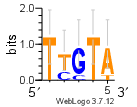
\includegraphics{cnu_bioinformatics_files/figure-pdf/cell-55-output-1.png}

\begin{itemize}
\tightlist
\item
  Position-weight matrices 계산
\item
  .counts 특성 사용
\end{itemize}

\begin{Shaded}
\begin{Highlighting}[]
\NormalTok{pwm }\OperatorTok{=}\NormalTok{ m.counts.normalize(pseudocounts}\OperatorTok{=}\FloatTok{0.5}\NormalTok{)}
\BuiltInTok{print}\NormalTok{(pwm)}
\end{Highlighting}
\end{Shaded}

\begin{verbatim}
        0      1      2      3      4
A:   0.19   0.81   0.06   0.56   0.81
C:   0.06   0.06   0.69   0.06   0.06
G:   0.06   0.06   0.19   0.31   0.06
T:   0.69   0.06   0.06   0.06   0.06
\end{verbatim}

\begin{Shaded}
\begin{Highlighting}[]
\NormalTok{pssm }\OperatorTok{=}\NormalTok{ pwm.log\_odds()}
\BuiltInTok{print}\NormalTok{(pssm)}
\end{Highlighting}
\end{Shaded}

\begin{verbatim}
        0      1      2      3      4
A:  -0.42   1.70  -2.00   1.17   1.70
C:  -2.00  -2.00   1.46  -2.00  -2.00
G:  -2.00  -2.00  -0.42   0.32  -2.00
T:   1.46  -2.00  -2.00  -2.00  -2.00
\end{verbatim}

\begin{Shaded}
\begin{Highlighting}[]
\NormalTok{background }\OperatorTok{=}\NormalTok{ \{}\StringTok{"A"}\NormalTok{:}\FloatTok{0.3}\NormalTok{,}\StringTok{"C"}\NormalTok{:}\FloatTok{0.2}\NormalTok{,}\StringTok{"G"}\NormalTok{:}\FloatTok{0.2}\NormalTok{,}\StringTok{"T"}\NormalTok{:}\FloatTok{0.3}\NormalTok{\}}
\NormalTok{pssm }\OperatorTok{=}\NormalTok{ pwm.log\_odds(background)}
\BuiltInTok{print}\NormalTok{(pssm)}
\end{Highlighting}
\end{Shaded}

\begin{verbatim}
        0      1      2      3      4
A:  -0.68   1.44  -2.26   0.91   1.44
C:  -1.68  -1.68   1.78  -1.68  -1.68
G:  -1.68  -1.68  -0.09   0.64  -1.68
T:   1.20  -2.26  -2.26  -2.26  -2.26
\end{verbatim}

\begin{itemize}
\tightlist
\item
  Using the PSSM score
\end{itemize}

\begin{Shaded}
\begin{Highlighting}[]
\ControlFlowTok{for}\NormalTok{ pos, score }\KeywordTok{in}\NormalTok{ pssm.search(test\_seq, threshold}\OperatorTok{=}\FloatTok{3.0}\NormalTok{):}
    \BuiltInTok{print}\NormalTok{(}\StringTok{"}\SpecialCharTok{\%d}\StringTok{, }\SpecialCharTok{\%f}\StringTok{ "} \OperatorTok{\%}\NormalTok{ (pos, score))}
\BuiltInTok{print}\NormalTok{(pssm.calculate(test\_seq))}
\end{Highlighting}
\end{Shaded}

\begin{verbatim}
0, 3.643981 
10, 6.759458 
[  3.643981    -8.560285    -2.4004133   -5.6533937   -4.2748823
  -0.05645879 -10.145247    -3.3293302   -5.9753222   -3.5703382
   6.759458    -5.3903594   -5.8598447   -0.81545067  -0.81545067
   0.7695118   -6.3903594   -3.5379167    0.4255574   -1.9309279
 -10.145247    -3.3293302 ]
\end{verbatim}

\includegraphics{PWMScanning.png}

\begin{Shaded}
\begin{Highlighting}[]
\NormalTok{m.pseudocounts }\OperatorTok{=} \FloatTok{0.1}
\BuiltInTok{print}\NormalTok{(m.counts)}
\BuiltInTok{print}\NormalTok{(m.pwm)}
\BuiltInTok{print}\NormalTok{(m.pssm)}
\end{Highlighting}
\end{Shaded}

\begin{verbatim}
        0      1      2      3      4
A:   1.00   6.00   0.00   4.00   6.00
C:   0.00   0.00   5.00   0.00   0.00
G:   0.00   0.00   1.00   2.00   0.00
T:   5.00   0.00   0.00   0.00   0.00

        0      1      2      3      4
A:   0.17   0.95   0.02   0.64   0.95
C:   0.02   0.02   0.80   0.02   0.02
G:   0.02   0.02   0.17   0.33   0.02
T:   0.80   0.02   0.02   0.02   0.02

        0      1      2      3      4
A:  -0.54   1.93  -4.00   1.36   1.93
C:  -4.00  -4.00   1.67  -4.00  -4.00
G:  -4.00  -4.00  -0.54   0.39  -4.00
T:   1.67  -4.00  -4.00  -4.00  -4.00
\end{verbatim}

\subsection{scikit-bio}\label{scikit-bio}

scikit-bio is another library focused on bioinformatics, providing
functionalities for sequence analysis, alignment, phylogenetics, and
more.

\subsubsection{Installation}\label{installation-2}

\begin{Shaded}
\begin{Highlighting}[]
\ExtensionTok{pip}\NormalTok{ install scikit{-}bio}
\end{Highlighting}
\end{Shaded}

\subsubsection{Basic Usage Examples}\label{basic-usage-examples}

\textbf{Reading and Writing Sequence Files:}

\begin{Shaded}
\begin{Highlighting}[]
\ImportTok{import}\NormalTok{ skbio}

\CommentTok{\# Reading a FASTA file}
\ControlFlowTok{for}\NormalTok{ seq }\KeywordTok{in}\NormalTok{ skbio.io.read(}\StringTok{"example.fasta"}\NormalTok{, }\BuiltInTok{format}\OperatorTok{=}\StringTok{"fasta"}\NormalTok{):}
    \BuiltInTok{print}\NormalTok{(seq.metadata[}\StringTok{\textquotesingle{}id\textquotesingle{}}\NormalTok{])}
    \BuiltInTok{print}\NormalTok{(seq)}

\CommentTok{\# Writing to a FASTA file}
\NormalTok{sequences }\OperatorTok{=}\NormalTok{ [seq }\ControlFlowTok{for}\NormalTok{ seq }\KeywordTok{in}\NormalTok{ skbio.io.read(}\StringTok{"example.fasta"}\NormalTok{, }\BuiltInTok{format}\OperatorTok{=}\StringTok{"fasta"}\NormalTok{)]}
\NormalTok{skbio.io.write(sequences, }\StringTok{"output.fasta"}\NormalTok{, }\BuiltInTok{format}\OperatorTok{=}\StringTok{"fasta"}\NormalTok{)}
\end{Highlighting}
\end{Shaded}

\textbf{Sequence Analysis:}

\begin{Shaded}
\begin{Highlighting}[]
\ImportTok{from}\NormalTok{ skbio }\ImportTok{import}\NormalTok{ DNA, RNA, Protein}

\CommentTok{\# Creating sequences}
\NormalTok{dna\_seq }\OperatorTok{=}\NormalTok{ DNA(}\StringTok{"AGTACACTGGT"}\NormalTok{)}
\NormalTok{rna\_seq }\OperatorTok{=}\NormalTok{ dna\_seq.transcribe()}
\NormalTok{protein\_seq }\OperatorTok{=}\NormalTok{ dna\_seq.translate()}

\BuiltInTok{print}\NormalTok{(}\StringTok{"DNA: "}\NormalTok{, dna\_seq)}
\BuiltInTok{print}\NormalTok{(}\StringTok{"RNA: "}\NormalTok{, rna\_seq)}
\BuiltInTok{print}\NormalTok{(}\StringTok{"Protein: "}\NormalTok{, protein\_seq)}
\end{Highlighting}
\end{Shaded}

\textbf{Alignment:}

\begin{Shaded}
\begin{Highlighting}[]
\ImportTok{from}\NormalTok{ skbio }\ImportTok{import}\NormalTok{ DNA}
\ImportTok{from}\NormalTok{ skbio.alignment }\ImportTok{import}\NormalTok{ local\_pairwise\_align\_ssw}

\NormalTok{seq1 }\OperatorTok{=}\NormalTok{ DNA(}\StringTok{"ACTGCTAGCTAG"}\NormalTok{)}
\NormalTok{seq2 }\OperatorTok{=}\NormalTok{ DNA(}\StringTok{"GCTAGCTAGGTA"}\NormalTok{)}

\NormalTok{alignment, score, start\_end\_positions }\OperatorTok{=}\NormalTok{ local\_pairwise\_align\_ssw(seq1, seq2)}

\BuiltInTok{print}\NormalTok{(}\StringTok{"Alignment:}\CharTok{\textbackslash{}n}\StringTok{"}\NormalTok{, alignment)}
\BuiltInTok{print}\NormalTok{(}\StringTok{"Score:"}\NormalTok{, score)}
\BuiltInTok{print}\NormalTok{(}\StringTok{"Start{-}End Positions:"}\NormalTok{, start\_end\_positions)}
\end{Highlighting}
\end{Shaded}

\textbf{Phylogenetic Tree Construction:}

\begin{Shaded}
\begin{Highlighting}[]
\ImportTok{from}\NormalTok{ skbio }\ImportTok{import}\NormalTok{ DistanceMatrix}
\ImportTok{from}\NormalTok{ skbio.tree }\ImportTok{import}\NormalTok{ nj}

\CommentTok{\# Example distance matrix}
\NormalTok{dm }\OperatorTok{=}\NormalTok{ DistanceMatrix([[}\FloatTok{0.0}\NormalTok{, }\FloatTok{0.2}\NormalTok{, }\FloatTok{0.4}\NormalTok{],}
\NormalTok{                     [}\FloatTok{0.2}\NormalTok{, }\FloatTok{0.0}\NormalTok{, }\FloatTok{0.6}\NormalTok{],}
\NormalTok{                     [}\FloatTok{0.4}\NormalTok{, }\FloatTok{0.6}\NormalTok{, }\FloatTok{0.0}\NormalTok{]],}
\NormalTok{                    [}\StringTok{\textquotesingle{}A\textquotesingle{}}\NormalTok{, }\StringTok{\textquotesingle{}B\textquotesingle{}}\NormalTok{, }\StringTok{\textquotesingle{}C\textquotesingle{}}\NormalTok{])}

\CommentTok{\# Constructing a phylogenetic tree using Neighbor{-}Joining}
\NormalTok{tree }\OperatorTok{=}\NormalTok{ nj(dm)}
\BuiltInTok{print}\NormalTok{(tree.ascii\_art())}
\end{Highlighting}
\end{Shaded}

\subsection{Example: Analyzing a Protein
Sequence}\label{example-analyzing-a-protein-sequence}

Let's put together an example that reads a protein sequence from a
GenBank file, performs some basic analysis using Biopython, and aligns
it using scikit-bio.

\begin{Shaded}
\begin{Highlighting}[]
\ImportTok{from}\NormalTok{ Bio }\ImportTok{import}\NormalTok{ SeqIO}
\ImportTok{from}\NormalTok{ Bio.Seq }\ImportTok{import}\NormalTok{ Seq}
\ImportTok{from}\NormalTok{ skbio }\ImportTok{import}\NormalTok{ Protein}
\ImportTok{from}\NormalTok{ skbio.alignment }\ImportTok{import}\NormalTok{ global\_pairwise\_align\_protein}

\CommentTok{\# Read a protein sequence from a GenBank file}
\NormalTok{record }\OperatorTok{=}\NormalTok{ SeqIO.read(}\StringTok{"example.gb"}\NormalTok{, }\StringTok{"genbank"}\NormalTok{)}
\NormalTok{protein\_seq }\OperatorTok{=}\NormalTok{ record.seq.translate()}

\BuiltInTok{print}\NormalTok{(}\StringTok{"Protein Sequence:"}\NormalTok{, protein\_seq)}

\CommentTok{\# Perform reverse translation to get the DNA sequence}
\NormalTok{dna\_seq }\OperatorTok{=}\NormalTok{ protein\_seq.reverse\_translate(table}\OperatorTok{=}\DecValTok{11}\NormalTok{)}
\BuiltInTok{print}\NormalTok{(}\StringTok{"Reverse Translated DNA Sequence:"}\NormalTok{, dna\_seq)}

\CommentTok{\# Perform alignment with another protein sequence}
\NormalTok{seq1 }\OperatorTok{=}\NormalTok{ Protein(}\BuiltInTok{str}\NormalTok{(protein\_seq))}
\NormalTok{seq2 }\OperatorTok{=}\NormalTok{ Protein(}\StringTok{"MKVLYNLKDG"}\NormalTok{)}

\NormalTok{alignment, score, start\_end\_positions }\OperatorTok{=}\NormalTok{ global\_pairwise\_align\_protein(seq1, seq2)}

\BuiltInTok{print}\NormalTok{(}\StringTok{"Alignment:}\CharTok{\textbackslash{}n}\StringTok{"}\NormalTok{, alignment)}
\BuiltInTok{print}\NormalTok{(}\StringTok{"Score:"}\NormalTok{, score)}
\BuiltInTok{print}\NormalTok{(}\StringTok{"Start{-}End Positions:"}\NormalTok{, start\_end\_positions)}
\end{Highlighting}
\end{Shaded}

\subsection{Explanation:}\label{explanation}

\begin{itemize}
\tightlist
\item
  \textbf{Reading Sequence}: We use Biopython to read a protein sequence
  from a GenBank file.
\item
  \textbf{Sequence Analysis}: We perform basic sequence operations like
  translation and reverse translation.
\item
  \textbf{Alignment}: We use scikit-bio to perform a global pairwise
  alignment between two protein sequences.
\end{itemize}

By mastering these bioinformatics libraries, you will be well-equipped
to handle a wide range of bioinformatics tasks and analyses in your
research. If you have specific questions or need further examples, feel
free to ask!

\bookmarksetup{startatroot}

\chapter{Machine Learning}\label{machine-learning}

\begin{Shaded}
\begin{Highlighting}[]
\ImportTok{import}\NormalTok{ os}

\NormalTok{os.chdir(}\StringTok{\textquotesingle{}drive/MyDrive/2024{-}cnu{-}lecture\textquotesingle{}}\NormalTok{)}
\end{Highlighting}
\end{Shaded}

\section{K-Nearest Neighbor (KNN)}\label{k-nearest-neighbor-knn}

\begin{itemize}
\tightlist
\item
  KNN은 지도학습의 한 종류로 거리 기반의 분류모델임
\item
  비지도학습의 클러스터링과 유사하나 Y값 (class, 반응값)이 있다는 점에서
  클러스터링과 차이
\item
  설명변수 X 값들을 이용해 반응변수 Y (분류)값을 설명하는 모형으로
\item
  새로운 데이터가 주어질 경우 K개의 인접한 데이터를 찾아서 이에 속한
  클래스로 분류 수행
\end{itemize}

\begin{Shaded}
\begin{Highlighting}[]
\ImportTok{import}\NormalTok{ numpy }\ImportTok{as}\NormalTok{ np}
\ImportTok{import}\NormalTok{ pandas }\ImportTok{as}\NormalTok{ pd}
\ImportTok{import}\NormalTok{ matplotlib.pyplot }\ImportTok{as}\NormalTok{ plt}

\ImportTok{from}\NormalTok{ sklearn.datasets }\ImportTok{import}\NormalTok{ load\_breast\_cancer}
\ImportTok{from}\NormalTok{ sklearn.metrics }\ImportTok{import}\NormalTok{ confusion\_matrix}
\ImportTok{from}\NormalTok{ sklearn.neighbors }\ImportTok{import}\NormalTok{ KNeighborsClassifier}
\ImportTok{from}\NormalTok{ sklearn.model\_selection }\ImportTok{import}\NormalTok{ train\_test\_split}

\ImportTok{import}\NormalTok{ seaborn }\ImportTok{as}\NormalTok{ sns}
\end{Highlighting}
\end{Shaded}

\begin{itemize}
\tightlist
\item
  https://github.com/HongleiXie/MLFromScratch
\item
  각종 ML 모형 (python, tensorflow 프레임워크)
\end{itemize}

\begin{Shaded}
\begin{Highlighting}[]
\NormalTok{breast\_cancer }\OperatorTok{=}\NormalTok{ load\_breast\_cancer()}
\end{Highlighting}
\end{Shaded}

\begin{Shaded}
\begin{Highlighting}[]
\BuiltInTok{dir}\NormalTok{(breast\_cancer)}
\BuiltInTok{print}\NormalTok{(breast\_cancer.DESCR)}
\end{Highlighting}
\end{Shaded}

\begin{Shaded}
\begin{Highlighting}[]
\BuiltInTok{print}\NormalTok{(breast\_cancer.data.shape)}
\NormalTok{X }\OperatorTok{=}\NormalTok{ pd.DataFrame(breast\_cancer.data, columns}\OperatorTok{=}\NormalTok{breast\_cancer.feature\_names)}
\NormalTok{X.head()}
\end{Highlighting}
\end{Shaded}

\begin{verbatim}
(569, 30)
\end{verbatim}

\begin{longtable}[]{@{}llllllllllllllllllllll@{}}
\toprule\noalign{}
& mean radius & mean texture & mean perimeter & mean area & mean
smoothness & mean compactness & mean concavity & mean concave points &
mean symmetry & mean fractal dimension & ... & worst radius & worst
texture & worst perimeter & worst area & worst smoothness & worst
compactness & worst concavity & worst concave points & worst symmetry &
worst fractal dimension \\
\midrule\noalign{}
\endhead
\bottomrule\noalign{}
\endlastfoot
0 & 17.99 & 10.38 & 122.80 & 1001.0 & 0.11840 & 0.27760 & 0.3001 &
0.14710 & 0.2419 & 0.07871 & ... & 25.38 & 17.33 & 184.60 & 2019.0 &
0.1622 & 0.6656 & 0.7119 & 0.2654 & 0.4601 & 0.11890 \\
1 & 20.57 & 17.77 & 132.90 & 1326.0 & 0.08474 & 0.07864 & 0.0869 &
0.07017 & 0.1812 & 0.05667 & ... & 24.99 & 23.41 & 158.80 & 1956.0 &
0.1238 & 0.1866 & 0.2416 & 0.1860 & 0.2750 & 0.08902 \\
2 & 19.69 & 21.25 & 130.00 & 1203.0 & 0.10960 & 0.15990 & 0.1974 &
0.12790 & 0.2069 & 0.05999 & ... & 23.57 & 25.53 & 152.50 & 1709.0 &
0.1444 & 0.4245 & 0.4504 & 0.2430 & 0.3613 & 0.08758 \\
3 & 11.42 & 20.38 & 77.58 & 386.1 & 0.14250 & 0.28390 & 0.2414 & 0.10520
& 0.2597 & 0.09744 & ... & 14.91 & 26.50 & 98.87 & 567.7 & 0.2098 &
0.8663 & 0.6869 & 0.2575 & 0.6638 & 0.17300 \\
4 & 20.29 & 14.34 & 135.10 & 1297.0 & 0.10030 & 0.13280 & 0.1980 &
0.10430 & 0.1809 & 0.05883 & ... & 22.54 & 16.67 & 152.20 & 1575.0 &
0.1374 & 0.2050 & 0.4000 & 0.1625 & 0.2364 & 0.07678 \\
\end{longtable}

\begin{itemize}
\tightlist
\item
  dummy y 변수 생성
\end{itemize}

\begin{Shaded}
\begin{Highlighting}[]
\NormalTok{y }\OperatorTok{=}\NormalTok{ pd.Categorical.from\_codes(breast\_cancer.target, breast\_cancer.target\_names)}
\NormalTok{y }\OperatorTok{=}\NormalTok{ pd.get\_dummies(y, drop\_first}\OperatorTok{=}\VariableTok{True}\NormalTok{)}
\NormalTok{y}
\end{Highlighting}
\end{Shaded}

\begin{longtable}[]{@{}ll@{}}
\toprule\noalign{}
& benign \\
\midrule\noalign{}
\endhead
\bottomrule\noalign{}
\endlastfoot
0 & False \\
1 & False \\
2 & False \\
3 & False \\
4 & False \\
... & ... \\
564 & False \\
565 & False \\
566 & False \\
567 & False \\
568 & True \\
\end{longtable}

\begin{itemize}
\tightlist
\item
  데이터셋 준비 (훈련/테스트셋)
\end{itemize}

\begin{Shaded}
\begin{Highlighting}[]
\NormalTok{X\_train, X\_test, y\_train, y\_test }\OperatorTok{=}\NormalTok{ train\_test\_split(X, y)}
\end{Highlighting}
\end{Shaded}

\begin{itemize}
\tightlist
\item
  모형 훈련 및 그래프
\end{itemize}

\begin{Shaded}
\begin{Highlighting}[]
\NormalTok{knn }\OperatorTok{=}\NormalTok{ KNeighborsClassifier(n\_neighbors}\OperatorTok{=}\DecValTok{5}\NormalTok{, metric}\OperatorTok{=}\StringTok{\textquotesingle{}euclidean\textquotesingle{}}\NormalTok{)}
\NormalTok{knn.fit(X\_train, y\_train)}
\NormalTok{y\_pred }\OperatorTok{=}\NormalTok{ knn.predict(X\_test)}
\NormalTok{sns.scatterplot(}
\NormalTok{    x}\OperatorTok{=}\StringTok{\textquotesingle{}mean area\textquotesingle{}}\NormalTok{,}
\NormalTok{    y}\OperatorTok{=}\StringTok{\textquotesingle{}mean compactness\textquotesingle{}}\NormalTok{,}
\NormalTok{    hue}\OperatorTok{=}\StringTok{\textquotesingle{}benign\textquotesingle{}}\NormalTok{,}
\NormalTok{    data}\OperatorTok{=}\NormalTok{X\_test.join(y\_test, how}\OperatorTok{=}\StringTok{\textquotesingle{}outer\textquotesingle{}}\NormalTok{)}
\NormalTok{)}
\end{Highlighting}
\end{Shaded}

\begin{verbatim}
/home/haseong/anaconda3/envs/biopy/lib/python3.11/site-packages/sklearn/neighbors/_classification.py:238: DataConversionWarning: A column-vector y was passed when a 1d array was expected. Please change the shape of y to (n_samples,), for example using ravel().
  return self._fit(X, y)
\end{verbatim}

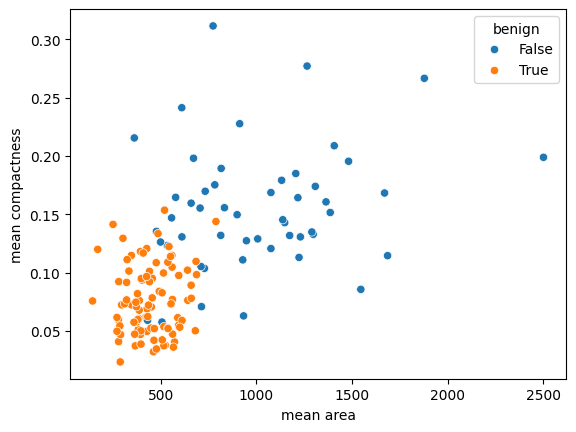
\includegraphics{cnu_machine_learning_files/figure-pdf/cell-9-output-2.png}

\begin{itemize}
\tightlist
\item
  예측 성능
\end{itemize}

\begin{Shaded}
\begin{Highlighting}[]
\NormalTok{results }\OperatorTok{=}\NormalTok{ pd.DataFrame([y\_test[}\StringTok{"benign"}\NormalTok{].values, y\_pred], index}\OperatorTok{=}\NormalTok{(}\StringTok{"test"}\NormalTok{, }\StringTok{"predict"}\NormalTok{)).T}
\BuiltInTok{print}\NormalTok{(results)}
\end{Highlighting}
\end{Shaded}

\begin{verbatim}
      test  predict
0    False     True
1     True     True
2    False    False
3    False    False
4     True     True
..     ...      ...
138  False    False
139  False    False
140   True     True
141   True     True
142   True     True

[143 rows x 2 columns]
\end{verbatim}

\begin{Shaded}
\begin{Highlighting}[]
\ImportTok{from}\NormalTok{ sklearn }\ImportTok{import}\NormalTok{ metrics}
\BuiltInTok{print}\NormalTok{(}\StringTok{"Accuracy:"}\NormalTok{,metrics.accuracy\_score(y\_test, y\_pred))}
\end{Highlighting}
\end{Shaded}

\begin{verbatim}
Accuracy: 0.9370629370629371
\end{verbatim}

\begin{itemize}
\tightlist
\item
  변수 중요도 탐색
\end{itemize}

\begin{Shaded}
\begin{Highlighting}[]
\ImportTok{from}\NormalTok{ sklearn.inspection }\ImportTok{import}\NormalTok{ permutation\_importance}

\CommentTok{\# Compute permutation feature importance}
\NormalTok{results }\OperatorTok{=}\NormalTok{ permutation\_importance(knn, X\_test, y\_test, n\_repeats}\OperatorTok{=}\DecValTok{5}\NormalTok{, random\_state}\OperatorTok{=}\DecValTok{40}\NormalTok{)}

\CommentTok{\# Get importance scores}
\NormalTok{feature\_importance }\OperatorTok{=}\NormalTok{ results.importances\_mean}

\CommentTok{\# Plot feature importance}
\NormalTok{plt.bar(}\BuiltInTok{range}\NormalTok{(X.shape[}\DecValTok{1}\NormalTok{]), feature\_importance, tick\_label}\OperatorTok{=}\NormalTok{breast\_cancer.feature\_names)}
\NormalTok{plt.xlabel(}\StringTok{\textquotesingle{}Features\textquotesingle{}}\NormalTok{)}
\NormalTok{plt.ylabel(}\StringTok{\textquotesingle{}Importance\textquotesingle{}}\NormalTok{)}
\NormalTok{plt.title(}\StringTok{\textquotesingle{}Feature Importance Using Permutation on Model\textquotesingle{}}\NormalTok{)}
\NormalTok{plt.xticks(rotation}\OperatorTok{=}\DecValTok{90}\NormalTok{)}
\NormalTok{plt.tight\_layout()}
\NormalTok{plt.show()}
\end{Highlighting}
\end{Shaded}

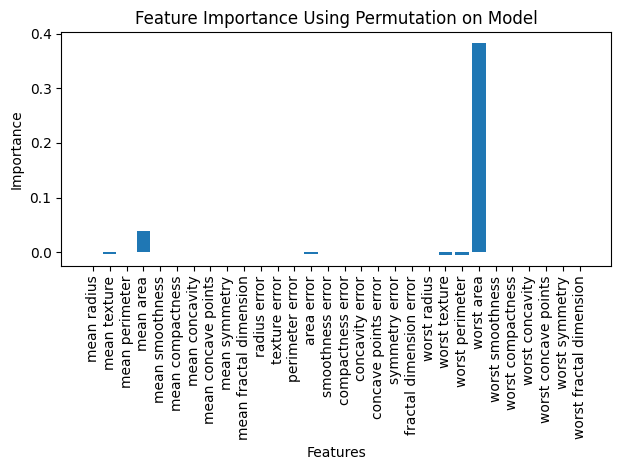
\includegraphics{cnu_machine_learning_files/figure-pdf/cell-12-output-1.png}

\bookmarksetup{startatroot}

\chapter{Deep Learning}\label{deep-learning}

\begin{Shaded}
\begin{Highlighting}[]
\ImportTok{import}\NormalTok{ os}

\NormalTok{os.chdir(}\StringTok{\textquotesingle{}drive/MyDrive/2024{-}cnu{-}lecture\textquotesingle{}}\NormalTok{)}
\end{Highlighting}
\end{Shaded}

\section{Convolutional Neual Network}\label{convolutional-neual-network}

\begin{itemize}
\tightlist
\item
  딥러닝 기반 DNA 서열 분석 가이드
\item
  http://www.btnews.or.kr/bbs/board.php?bo\_table=bt\_news\&wr\_id=342
\end{itemize}

\subsection{목표}\label{uxbaa9uxd45c}

\begin{itemize}
\tightlist
\item
  임의의 활성을 갖는 서열을 분류하는 CNN 모형 개발 (시뮬레이션)
\item
  예시) 임의의 전사인자가 결합하는 특정 DNA 모티프 찾는 모형 개발. 즉,
  모형 개발 후 임의의 DNA 서열을 모형에 넣었을 때 해당 전사인자가 입력
  DNA 서열에 붙으면 1 붙지 않으면 0 이라고 예측하는 모형 개발
\end{itemize}

\subsection{데이터}\label{uxb370uxc774uxd130}

딥러닝을 위해서는 라벨링 데이터가 필요함 (최근 self-supervised
learning에서는 필수는 아님). 서열분석의 경우에는 DNA 서열과 함께 해당
서열의 표현형이 라벨이 될 수 있음 (Genotype-phenotype 짝 데이터). 예를
들어 특정 전사인자가 결합하는 DNA 서열을 예측하는 딥러닝 모형을
학습하고자 할 경우 전사인자의 서열 데이터와 해당 전사인자가 DNA에 실제로
붙는지를 나타내는 True 또는 False 라벨이 붙은 데이터가 필요함.

일반적으로 통계적 분석을 위한 데이터는 샘플의 개수와 (행) 변수의 개수로
(열) 구분되어 2차원 배열 형태로 표현. 딥러닝에서도 같은 방식으로
데이터를 표현하며 필요한 샘플의 수는 학습할 모형의 복잡도에 따라서
달라질 수 있지만 최소 수천 개 이상이 필요하며 수 만개 이상의 가능한 많은
데이터를 사용 권장.

딥러닝을 위해서 수집된 데이터 세트는 모형 학습을 위한 Training 데이터와
Test 데이터로 나누어 사용되며 Training 데이터는 또다시 Training 데이터와
Validation 데이터로 나누어 구분.

\subsection{One-hot encoding}\label{one-hot-encoding}

딥러닝을 위해서 데이터는 숫자(기계가 인식 가능한)로 표현 필요. One-hot
encoding은 딥러닝에서 가장 널리 사용되는 방법 중 하나이며 4 종류의
염기를 갖는 DNA의 경우 ``A''는 {[}1,0,0,0{]}, ``T''는 {[}0,0,0,1{]},
``G''는 {[}0,0,1,0{]}, 그리고 ``C''는 {[}0,1,0,0{]} 으로 인코딩 할 수
있음

\begin{Shaded}
\begin{Highlighting}[]
\ImportTok{import}\NormalTok{ numpy }\ImportTok{as}\NormalTok{ np}

\NormalTok{my\_string}\OperatorTok{=}\StringTok{"ATACAA"}
\NormalTok{my\_array}\OperatorTok{=}\NormalTok{np.array(}\BuiltInTok{list}\NormalTok{(my\_string))}
\BuiltInTok{print}\NormalTok{(my\_array)}
\end{Highlighting}
\end{Shaded}

\begin{verbatim}
['A' 'T' 'A' 'C' 'A' 'A']
\end{verbatim}

\begin{Shaded}
\begin{Highlighting}[]
\BuiltInTok{list}\NormalTok{(my\_string)}
\end{Highlighting}
\end{Shaded}

\begin{verbatim}
['A', 'T', 'A', 'C', 'A', 'A']
\end{verbatim}

\begin{itemize}
\tightlist
\item
  Numpy Dimension 관련 내용은 앞서 강의 numpy 부분 참고
\end{itemize}

\begin{Shaded}
\begin{Highlighting}[]
\NormalTok{display(np.zeros(}\DecValTok{5}\NormalTok{))}
\NormalTok{display(np.zeros((}\DecValTok{7}\NormalTok{,}\DecValTok{5}\NormalTok{)))}
\end{Highlighting}
\end{Shaded}

\begin{verbatim}
array([0., 0., 0., 0., 0.])
\end{verbatim}

\begin{verbatim}
array([[0., 0., 0., 0., 0.],
       [0., 0., 0., 0., 0.],
       [0., 0., 0., 0., 0.],
       [0., 0., 0., 0., 0.],
       [0., 0., 0., 0., 0.],
       [0., 0., 0., 0., 0.],
       [0., 0., 0., 0., 0.]])
\end{verbatim}

\begin{Shaded}
\begin{Highlighting}[]
\NormalTok{box }\OperatorTok{=}\NormalTok{ np.zeros((}\DecValTok{3}\NormalTok{, }\DecValTok{7}\NormalTok{, }\DecValTok{5}\NormalTok{))}
\BuiltInTok{type}\NormalTok{(box)}
\end{Highlighting}
\end{Shaded}

\begin{verbatim}
numpy.ndarray
\end{verbatim}

\begin{Shaded}
\begin{Highlighting}[]
\NormalTok{onehot\_encode }\OperatorTok{=}\NormalTok{ np.zeros((}\BuiltInTok{len}\NormalTok{(my\_array),}\DecValTok{4}\NormalTok{), dtype}\OperatorTok{=}\BuiltInTok{int}\NormalTok{)}
\NormalTok{base\_dict }\OperatorTok{=}\NormalTok{ \{}\StringTok{"A"}\NormalTok{:}\DecValTok{0}\NormalTok{, }\StringTok{"C"}\NormalTok{:}\DecValTok{1}\NormalTok{, }\StringTok{"G"}\NormalTok{:}\DecValTok{2}\NormalTok{, }\StringTok{"T"}\NormalTok{:}\DecValTok{3}\NormalTok{\}}
\ControlFlowTok{for}\NormalTok{ i }\KeywordTok{in} \BuiltInTok{range}\NormalTok{(}\BuiltInTok{len}\NormalTok{(my\_array)):}
\NormalTok{    onehot\_encode[i, base\_dict[my\_array[i]]] }\OperatorTok{=} \DecValTok{1}

\BuiltInTok{print}\NormalTok{(onehot\_encode)}
\BuiltInTok{print}\NormalTok{(onehot\_encode.shape)}
\end{Highlighting}
\end{Shaded}

\begin{verbatim}
[[1 0 0 0]
 [0 0 0 1]
 [1 0 0 0]
 [0 1 0 0]
 [1 0 0 0]
 [1 0 0 0]]
(6, 4)
\end{verbatim}

\begin{itemize}
\tightlist
\item
  one-hot 방식으로 변환한 서열 데이터
\end{itemize}

\begin{figure}[H]

{\centering 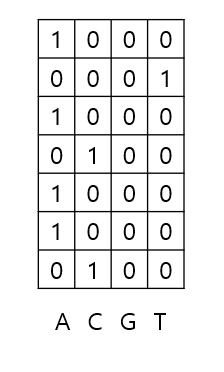
\includegraphics{images/64dm.png}

}

\caption{alt text}

\end{figure}%

\subsection{모티프 설정}\label{uxbaa8uxd2f0uxd504-uxc124uxc815}

PFM (Position Frequency Matrix)와 PWM (Position Weight Matrix) 개념 이해
필요. Alignment가 수행된 몇 개의 서열들을 가정하면 PFM은 이 서열들의
특정 위치에 A, T, G, C 각 염기들의 빈도수를 나타내며 PWM은 각 염기의
비율을 나타냄.

\begin{Shaded}
\begin{Highlighting}[]
\ImportTok{from}\NormalTok{ Bio }\ImportTok{import}\NormalTok{ motifs}
\ImportTok{from}\NormalTok{ Bio.Seq }\ImportTok{import}\NormalTok{ Seq}

\NormalTok{instances }\OperatorTok{=}\NormalTok{ [Seq(}\StringTok{"TACAA"}\NormalTok{), Seq(}\StringTok{"TACGA"}\NormalTok{), Seq(}\StringTok{"TACAA"}\NormalTok{)]}
\NormalTok{m }\OperatorTok{=}\NormalTok{ motifs.create(instances)}
\NormalTok{pfm }\OperatorTok{=}\NormalTok{ m.counts}
\BuiltInTok{print}\NormalTok{(pfm)}
\NormalTok{pwm }\OperatorTok{=}\NormalTok{ m.counts.normalize(pseudocounts}\OperatorTok{=}\FloatTok{0.5}\NormalTok{)}
\BuiltInTok{print}\NormalTok{ (pwm)}
\end{Highlighting}
\end{Shaded}

\begin{verbatim}
        0      1      2      3      4
A:   0.00   3.00   0.00   2.00   3.00
C:   0.00   0.00   3.00   0.00   0.00
G:   0.00   0.00   0.00   1.00   0.00
T:   3.00   0.00   0.00   0.00   0.00

        0      1      2      3      4
A:   0.10   0.70   0.10   0.50   0.70
C:   0.10   0.10   0.70   0.10   0.10
G:   0.10   0.10   0.10   0.30   0.10
T:   0.70   0.10   0.10   0.10   0.10
\end{verbatim}

pseudocounts는 계산시 NULL이나 0으로 나누어지는 경우 방지. 특정 서열
모티프의 PWM은 새로운 서열이 One-hot encoding 방식으로 주어져 있을 경우
서열 처음 위치부터 마지막까지 Sliding window 방식으로 해당 모티프가 있는
위치를 탐색할 수 있음. 다음은 위 주어진 pwm모티프를 0, 1로만 가정하여
해당 모티프의 존재 유무를 계산하는 방법을 보여줌.

\begin{figure}[H]

{\centering 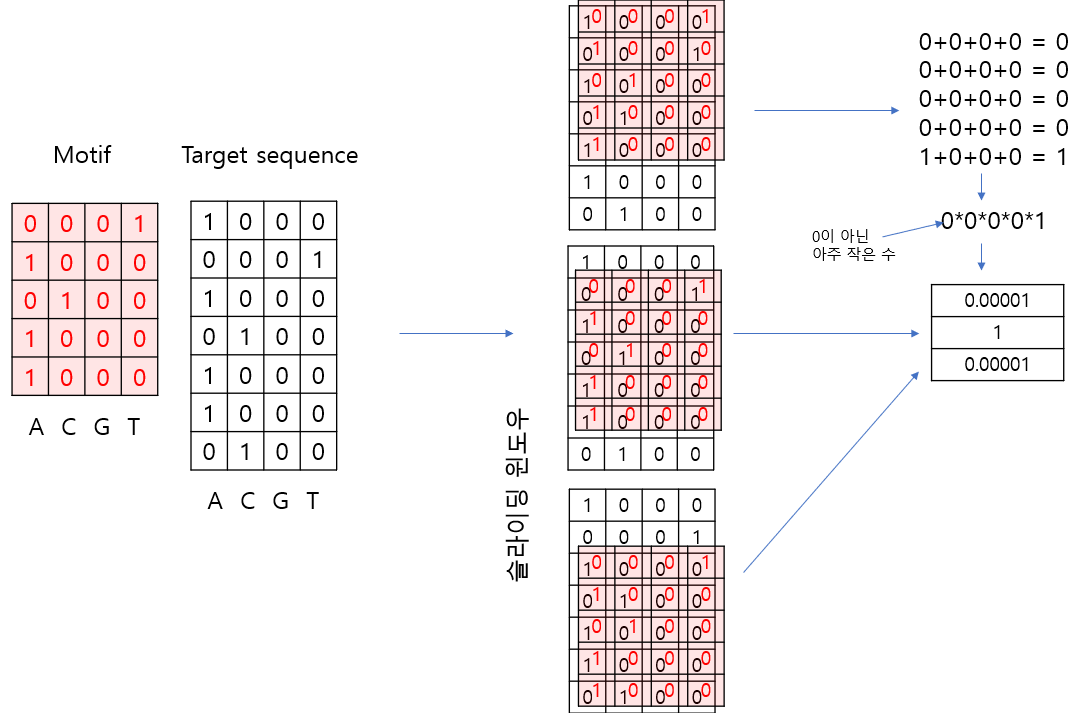
\includegraphics{images/sliding_window.png}

}

\caption{alt text}

\end{figure}%

위와 같이 길이3 배열에 1이 있을 경우 타깃 서열에 모티프와 같은 서열이
있음을 알 수 있음

앞서 ``ATACAA'' 서열에서 위 PWM 모티프가 존재하는지 탐색. ``ATACAA'' 는
길이 5인 슬라이딩 윈도우를 사용하면 ``ATACA''와 ``TACAA'' 두 개의 서열로
나눌 수 있음. 이 두 서열을 One-hot encoding으로 전환 후 위 PWM과
원소들끼리 곱하면 One-hot encoding에서 0이 아닌 위치와 동일 위치의 PWM
값들만 남게 되므로 0이 아닌 값들을 모두 곱한 후 log를 취해 주면 해당
서열이 모티프와 얼마나 비슷한지를 나타내는 스칼라 값이 구해짐.
이론적으로 이 값이 0이면 동일한 서열임.

\begin{Shaded}
\begin{Highlighting}[]
\NormalTok{pwm\_arr }\OperatorTok{=}\NormalTok{ np.array(}\BuiltInTok{list}\NormalTok{(pwm.values())).transpose()}
\BuiltInTok{print}\NormalTok{(pwm\_arr.shape)}

\BuiltInTok{print}\NormalTok{(onehot\_encode.shape)}
\BuiltInTok{print}\NormalTok{(onehot\_encode[}\DecValTok{0}\NormalTok{:}\DecValTok{5}\NormalTok{,].shape)}
\BuiltInTok{print}\NormalTok{(onehot\_encode[}\DecValTok{1}\NormalTok{:}\DecValTok{6}\NormalTok{,].shape)}

\NormalTok{s1 }\OperatorTok{=}\NormalTok{ np.multiply(onehot\_encode[}\DecValTok{0}\NormalTok{:}\DecValTok{5}\NormalTok{,], pwm\_arr)}
\NormalTok{s2 }\OperatorTok{=}\NormalTok{ np.multiply(onehot\_encode[}\DecValTok{1}\NormalTok{:}\DecValTok{6}\NormalTok{,], pwm\_arr)}
\BuiltInTok{print}\NormalTok{(s1)}
\BuiltInTok{print}\NormalTok{(s2)}

\BuiltInTok{print}\NormalTok{(np.}\BuiltInTok{sum}\NormalTok{(s1, axis}\OperatorTok{=}\DecValTok{1}\NormalTok{))}
\BuiltInTok{print}\NormalTok{(np.prod(np.}\BuiltInTok{sum}\NormalTok{(s1, axis}\OperatorTok{=}\DecValTok{1}\NormalTok{)))}

\BuiltInTok{print}\NormalTok{(np.log(np.prod(np.}\BuiltInTok{sum}\NormalTok{(s1, axis}\OperatorTok{=}\DecValTok{1}\NormalTok{)))) }\CommentTok{\#s1 score}
\BuiltInTok{print}\NormalTok{(np.log(np.prod(np.}\BuiltInTok{sum}\NormalTok{(s2, axis}\OperatorTok{=}\DecValTok{1}\NormalTok{)))) }\CommentTok{\#s2 score}
\end{Highlighting}
\end{Shaded}

\begin{verbatim}
(5, 4)
(6, 4)
(5, 4)
(5, 4)
[[0.1 0.  0.  0. ]
 [0.  0.  0.  0.1]
 [0.1 0.  0.  0. ]
 [0.  0.1 0.  0. ]
 [0.7 0.  0.  0. ]]
[[0.  0.  0.  0.7]
 [0.7 0.  0.  0. ]
 [0.  0.7 0.  0. ]
 [0.5 0.  0.  0. ]
 [0.7 0.  0.  0. ]]
[0.1 0.1 0.1 0.1 0.7]
7.000000000000002e-05
-9.567015315914915
-2.119846956314875
\end{verbatim}

\begin{itemize}
\tightlist
\item
  딥러닝 스타일로 배열을 가시화 할 경우 다음과 같이 표현 가능
\end{itemize}

\begin{figure}[H]

{\centering 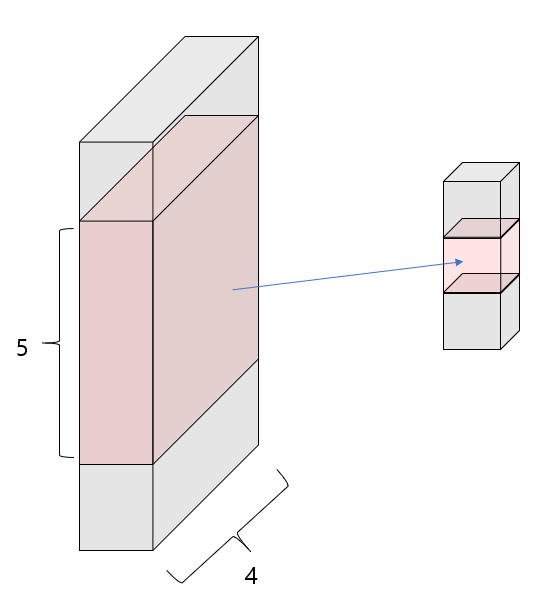
\includegraphics{images/deeplearning_dim.png}

}

\caption{alt text}

\end{figure}%

\section{모의 서열 데이터
생성}\label{uxbaa8uxc758-uxc11cuxc5f4-uxb370uxc774uxd130-uxc0dduxc131}

서열 중간 motif를 넣어서 임의의 시뮬레이션 positive 데이터를 1000개
생성하고 랜덤한 서열을 넣어 negative 데이터를 1000개 생성함

\begin{Shaded}
\begin{Highlighting}[]
\ImportTok{import}\NormalTok{ numpy }\ImportTok{as}\NormalTok{ np}
\NormalTok{seq\_length }\OperatorTok{=} \DecValTok{20}
\NormalTok{num\_sample }\OperatorTok{=} \DecValTok{1000}
\CommentTok{\#motif CCGGAA}
\NormalTok{motif\_pwm }\OperatorTok{=}\NormalTok{ np.array([[}\FloatTok{10.41}\NormalTok{, }\FloatTok{22.86}\NormalTok{, }\FloatTok{1.92}\NormalTok{, }\FloatTok{1.55}\NormalTok{, }\FloatTok{98.60}\NormalTok{, }\FloatTok{86.66}\NormalTok{],}
\NormalTok{            [}\FloatTok{68.20}\NormalTok{, }\FloatTok{65.25}\NormalTok{, }\FloatTok{0.50}\NormalTok{, }\FloatTok{0.35}\NormalTok{, }\FloatTok{0.25}\NormalTok{, }\FloatTok{2.57}\NormalTok{],}
\NormalTok{            [}\FloatTok{17.27}\NormalTok{, }\FloatTok{8.30}\NormalTok{, }\FloatTok{94.77}\NormalTok{, }\FloatTok{97.32}\NormalTok{, }\FloatTok{0.87}\NormalTok{, }\FloatTok{0.00}\NormalTok{],}
\NormalTok{            [}\FloatTok{4.13}\NormalTok{, }\FloatTok{3.59}\NormalTok{, }\FloatTok{2.81}\NormalTok{, }\FloatTok{0.78}\NormalTok{, }\FloatTok{0.28}\NormalTok{, }\FloatTok{10.77}\NormalTok{]])}
\NormalTok{pwm }\OperatorTok{=}\NormalTok{ np.hstack([np.ones((}\DecValTok{4}\NormalTok{, }\DecValTok{7}\NormalTok{)), motif\_pwm, np.ones((}\DecValTok{4}\NormalTok{, }\DecValTok{7}\NormalTok{))])}
\NormalTok{pos }\OperatorTok{=}\NormalTok{ np.array([np.random.choice( [}\StringTok{\textquotesingle{}A\textquotesingle{}}\NormalTok{, }\StringTok{\textquotesingle{}C\textquotesingle{}}\NormalTok{, }\StringTok{\textquotesingle{}G\textquotesingle{}}\NormalTok{, }\StringTok{\textquotesingle{}T\textquotesingle{}}\NormalTok{], num\_sample,}
\NormalTok{                                  p}\OperatorTok{=}\NormalTok{pwm[:,i]}\OperatorTok{/}\BuiltInTok{sum}\NormalTok{(pwm[:,i])) }\ControlFlowTok{for}\NormalTok{ i }\KeywordTok{in} \BuiltInTok{range}\NormalTok{(seq\_length)]).transpose()}
\NormalTok{neg }\OperatorTok{=}\NormalTok{ np.array([np.random.choice( [}\StringTok{\textquotesingle{}A\textquotesingle{}}\NormalTok{, }\StringTok{\textquotesingle{}C\textquotesingle{}}\NormalTok{, }\StringTok{\textquotesingle{}G\textquotesingle{}}\NormalTok{, }\StringTok{\textquotesingle{}T\textquotesingle{}}\NormalTok{], num\_sample,}
\NormalTok{                                  p}\OperatorTok{=}\NormalTok{np.array([}\DecValTok{1}\NormalTok{,}\DecValTok{1}\NormalTok{,}\DecValTok{1}\NormalTok{,}\DecValTok{1}\NormalTok{])}\OperatorTok{/}\DecValTok{4}\NormalTok{) }\ControlFlowTok{for}\NormalTok{ i }\KeywordTok{in} \BuiltInTok{range}\NormalTok{(seq\_length)]).transpose()}

\BuiltInTok{print}\NormalTok{(pos.shape)}
\NormalTok{display([}\StringTok{\textquotesingle{}\textquotesingle{}}\NormalTok{.join(x) }\ControlFlowTok{for}\NormalTok{ x }\KeywordTok{in}\NormalTok{ pos[}\DecValTok{1}\NormalTok{:}\DecValTok{5}\NormalTok{,]])}
\BuiltInTok{print}\NormalTok{()}
\NormalTok{display([}\StringTok{\textquotesingle{}\textquotesingle{}}\NormalTok{.join(x) }\ControlFlowTok{for}\NormalTok{ x }\KeywordTok{in}\NormalTok{ neg[}\DecValTok{1}\NormalTok{:}\DecValTok{5}\NormalTok{,]])}
\end{Highlighting}
\end{Shaded}

\begin{verbatim}
(1000, 20)
\end{verbatim}

\begin{verbatim}
['AGCGTAGGCGGAACATAATA',
 'GGATCGTCAGGATCACCGCC',
 'CCGAGTCACGGAATTAACTG',
 'AACATCAGCGGAAGCTTTGT']
\end{verbatim}

\begin{verbatim}
['TTCCAATTACCGACCTGGAT',
 'ATTGATTTCCTGCCAAGATC',
 'AGTGAGCTGCTTTAGGTCCC',
 'TGTGAGGGCTTAGATGAATG']
\end{verbatim}

\subsection{DNA 서열 데이터
전처리}\label{dna-uxc11cuxc5f4-uxb370uxc774uxd130-uxc804uxcc98uxb9ac}

\begin{Shaded}
\begin{Highlighting}[]
\NormalTok{base\_dict }\OperatorTok{=}\NormalTok{ \{}\StringTok{\textquotesingle{}A\textquotesingle{}}\NormalTok{:}\DecValTok{0}\NormalTok{, }\StringTok{\textquotesingle{}C\textquotesingle{}}\NormalTok{:}\DecValTok{1}\NormalTok{, }\StringTok{\textquotesingle{}G\textquotesingle{}}\NormalTok{:}\DecValTok{2}\NormalTok{, }\StringTok{\textquotesingle{}T\textquotesingle{}}\NormalTok{:}\DecValTok{3}\NormalTok{\}}

\CommentTok{\# response variable for pos}
\NormalTok{onehot\_encode\_pos }\OperatorTok{=}\NormalTok{ np.zeros((num\_sample, seq\_length, }\DecValTok{4}\NormalTok{))}
\NormalTok{onehot\_encode\_pos\_label }\OperatorTok{=}\NormalTok{ np.zeros((num\_sample, }\DecValTok{2}\NormalTok{), dtype}\OperatorTok{=}\BuiltInTok{int}\NormalTok{)}
\NormalTok{onehot\_encode\_pos\_label[:,}\DecValTok{0}\NormalTok{] }\OperatorTok{=} \DecValTok{1}
\CommentTok{\# print(onehot\_encode\_pos\_label)}

\CommentTok{\# response variable for pos}
\NormalTok{onehot\_encode\_neg }\OperatorTok{=}\NormalTok{ np.zeros((num\_sample, seq\_length, }\DecValTok{4}\NormalTok{))}
\NormalTok{onehot\_encode\_neg\_label }\OperatorTok{=}\NormalTok{ np.zeros((num\_sample, }\DecValTok{2}\NormalTok{), dtype}\OperatorTok{=}\BuiltInTok{int}\NormalTok{)}
\NormalTok{onehot\_encode\_neg\_label[:,}\DecValTok{1}\NormalTok{] }\OperatorTok{=} \DecValTok{1}
\CommentTok{\# print(onehot\_encode\_neg\_label)}

\CommentTok{\# convert sequence to onehot}
\ControlFlowTok{for}\NormalTok{ i }\KeywordTok{in} \BuiltInTok{range}\NormalTok{(num\_sample):}
    \ControlFlowTok{for}\NormalTok{ j }\KeywordTok{in} \BuiltInTok{range}\NormalTok{(seq\_length):}
\NormalTok{        onehot\_encode\_pos[i,j,base\_dict[pos[i,j]]] }\OperatorTok{=} \DecValTok{1}
\NormalTok{        onehot\_encode\_neg[i,j,base\_dict[neg[i,j]]] }\OperatorTok{=} \DecValTok{1}

\CommentTok{\# concatenation}
\NormalTok{X }\OperatorTok{=}\NormalTok{ np.vstack((onehot\_encode\_pos, onehot\_encode\_neg))}
\NormalTok{y }\OperatorTok{=}\NormalTok{ np.vstack((onehot\_encode\_pos\_label, onehot\_encode\_neg\_label))}

\BuiltInTok{print}\NormalTok{(X.shape, y.shape)}
\CommentTok{\# (2000, 20, 4) (2000, 2)}
\end{Highlighting}
\end{Shaded}

\begin{verbatim}
(2000, 20, 4) (2000, 2)
\end{verbatim}

\begin{itemize}
\tightlist
\item
  PyTorch Conv1d는 입력 데이터가 {[}batch\_size, channels, length{]}의
  형식이므로 transpose(1,2) 적용
\end{itemize}

\begin{Shaded}
\begin{Highlighting}[]
\ImportTok{import}\NormalTok{ torch}
\ImportTok{from}\NormalTok{ torch.utils.data }\ImportTok{import}\NormalTok{ TensorDataset, DataLoader}
\ImportTok{from}\NormalTok{ sklearn.model\_selection }\ImportTok{import}\NormalTok{ train\_test\_split}

\CommentTok{\# 데이터를 훈련 세트와 테스트 세트로 나눔}
\NormalTok{X\_train, X\_test, y\_train, y\_test }\OperatorTok{=}\NormalTok{ train\_test\_split(X, y, test\_size}\OperatorTok{=}\FloatTok{0.2}\NormalTok{, random\_state}\OperatorTok{=}\DecValTok{125}\NormalTok{)}
\BuiltInTok{print}\NormalTok{(X\_train.shape, y\_train.shape)}

\CommentTok{\# NumPy 배열을 PyTorch 텐서로 변환}
\NormalTok{X\_train }\OperatorTok{=}\NormalTok{ torch.tensor(X\_train, dtype}\OperatorTok{=}\NormalTok{torch.float32).transpose(}\DecValTok{1}\NormalTok{,}\DecValTok{2}\NormalTok{)}
\NormalTok{X\_test }\OperatorTok{=}\NormalTok{ torch.tensor(X\_test, dtype}\OperatorTok{=}\NormalTok{torch.float32).transpose(}\DecValTok{1}\NormalTok{,}\DecValTok{2}\NormalTok{)}
\NormalTok{y\_train }\OperatorTok{=}\NormalTok{ torch.tensor(y\_train, dtype}\OperatorTok{=}\NormalTok{torch.float32)}
\NormalTok{y\_test }\OperatorTok{=}\NormalTok{ torch.tensor(y\_test, dtype}\OperatorTok{=}\NormalTok{torch.float32)}
\BuiltInTok{print}\NormalTok{(y\_test.dtype)}

\CommentTok{\# DataLoader 설정}
\NormalTok{train\_dataset }\OperatorTok{=}\NormalTok{ TensorDataset(X\_train, y\_train)}
\NormalTok{train\_loader }\OperatorTok{=}\NormalTok{ DataLoader(train\_dataset, batch\_size}\OperatorTok{=}\DecValTok{64}\NormalTok{, shuffle}\OperatorTok{=}\VariableTok{True}\NormalTok{)}
\BuiltInTok{print}\NormalTok{(train\_loader.dataset.tensors[}\DecValTok{0}\NormalTok{].shape)}
\BuiltInTok{print}\NormalTok{(train\_loader.dataset.tensors[}\DecValTok{1}\NormalTok{].shape)}
\NormalTok{test\_dataset }\OperatorTok{=}\NormalTok{ TensorDataset(X\_test, y\_test)}
\NormalTok{test\_loader }\OperatorTok{=}\NormalTok{ DataLoader(test\_dataset, batch\_size}\OperatorTok{=}\DecValTok{64}\NormalTok{, shuffle}\OperatorTok{=}\VariableTok{False}\NormalTok{)}
\end{Highlighting}
\end{Shaded}

\begin{verbatim}
(1600, 20, 4) (1600, 2)
torch.float32
torch.Size([1600, 4, 20])
torch.Size([1600, 2])
\end{verbatim}

\begin{Shaded}
\begin{Highlighting}[]
\ImportTok{import}\NormalTok{ torch}

\NormalTok{X\_torch }\OperatorTok{=}\NormalTok{ torch.tensor(X\_train, dtype}\OperatorTok{=}\NormalTok{torch.float32)}
\BuiltInTok{print}\NormalTok{(X\_torch.shape)}
\end{Highlighting}
\end{Shaded}

\begin{verbatim}
torch.Size([1600, 4, 20])
\end{verbatim}

\begin{verbatim}
/tmp/ipykernel_341094/3124571761.py:3: UserWarning: To copy construct from a tensor, it is recommended to use sourceTensor.clone().detach() or sourceTensor.clone().detach().requires_grad_(True), rather than torch.tensor(sourceTensor).
  X_torch = torch.tensor(X_train, dtype=torch.float32)
\end{verbatim}

\section{모델 정의}\label{uxbaa8uxb378-uxc815uxc758}

\begin{Shaded}
\begin{Highlighting}[]
\ImportTok{import}\NormalTok{ torch.nn }\ImportTok{as}\NormalTok{ nn}
\ImportTok{import}\NormalTok{ torch.optim }\ImportTok{as}\NormalTok{ optim}

\ImportTok{import}\NormalTok{ torch}
\ImportTok{import}\NormalTok{ torch.nn }\ImportTok{as}\NormalTok{ nn}
\ImportTok{import}\NormalTok{ torch.optim }\ImportTok{as}\NormalTok{ optim}

\KeywordTok{class}\NormalTok{ DNA\_CNN(nn.Module):}
    \KeywordTok{def} \FunctionTok{\_\_init\_\_}\NormalTok{(}\VariableTok{self}\NormalTok{):}
        \BuiltInTok{super}\NormalTok{(DNA\_CNN, }\VariableTok{self}\NormalTok{).}\FunctionTok{\_\_init\_\_}\NormalTok{()}
        \VariableTok{self}\NormalTok{.conv1 }\OperatorTok{=}\NormalTok{ nn.Conv1d(in\_channels}\OperatorTok{=}\DecValTok{4}\NormalTok{, out\_channels}\OperatorTok{=}\DecValTok{16}\NormalTok{, kernel\_size}\OperatorTok{=}\DecValTok{3}\NormalTok{, padding}\OperatorTok{=}\DecValTok{1}\NormalTok{)}
        \VariableTok{self}\NormalTok{.relu }\OperatorTok{=}\NormalTok{ nn.ReLU()}
        \VariableTok{self}\NormalTok{.maxpool }\OperatorTok{=}\NormalTok{ nn.MaxPool1d(kernel\_size}\OperatorTok{=}\DecValTok{2}\NormalTok{)}
        \VariableTok{self}\NormalTok{.flatten }\OperatorTok{=}\NormalTok{ nn.Flatten()}
        \VariableTok{self}\NormalTok{.fc1 }\OperatorTok{=}\NormalTok{ nn.Linear(}\DecValTok{160}\NormalTok{, }\DecValTok{64}\NormalTok{)  }\CommentTok{\# Adjust the input features according to your pooling and conv1d output}
        \VariableTok{self}\NormalTok{.fc2 }\OperatorTok{=}\NormalTok{ nn.Linear(}\DecValTok{64}\NormalTok{, }\DecValTok{2}\NormalTok{)  }\CommentTok{\# Adjust according to your problem\textquotesingle{}s needs (e.g., number of classes)}
        \CommentTok{\#self.softmax = nn.Softmax(dim=1)}

    \KeywordTok{def}\NormalTok{ forward(}\VariableTok{self}\NormalTok{, x):}
\NormalTok{        x }\OperatorTok{=} \VariableTok{self}\NormalTok{.conv1(x)}
\NormalTok{        x }\OperatorTok{=} \VariableTok{self}\NormalTok{.relu(x)}
\NormalTok{        x }\OperatorTok{=} \VariableTok{self}\NormalTok{.maxpool(x)}
\NormalTok{        x }\OperatorTok{=} \VariableTok{self}\NormalTok{.flatten(x)}
\NormalTok{        x }\OperatorTok{=} \VariableTok{self}\NormalTok{.fc1(x)}
\NormalTok{        x }\OperatorTok{=} \VariableTok{self}\NormalTok{.fc2(x)}
        \CommentTok{\#x = self.softmax(x)}
        \ControlFlowTok{return}\NormalTok{ x}

\NormalTok{model }\OperatorTok{=}\NormalTok{ DNA\_CNN()}
\ControlFlowTok{if}\NormalTok{ torch.cuda.is\_available():}
\NormalTok{    model.cuda()}

\CommentTok{\# Loss and optimizer}
\NormalTok{criterion }\OperatorTok{=}\NormalTok{ nn.CrossEntropyLoss()}
\NormalTok{optimizer }\OperatorTok{=}\NormalTok{ optim.Adam(model.parameters(), lr}\OperatorTok{=}\FloatTok{0.001}\NormalTok{)}

\ImportTok{from}\NormalTok{ torchsummary }\ImportTok{import}\NormalTok{ summary}
\NormalTok{summary(model, input\_size}\OperatorTok{=}\NormalTok{(}\DecValTok{4}\NormalTok{, }\DecValTok{20}\NormalTok{))  }\CommentTok{\# (Channels, Length)}
\end{Highlighting}
\end{Shaded}

\begin{verbatim}
----------------------------------------------------------------
        Layer (type)               Output Shape         Param #
================================================================
            Conv1d-1               [-1, 16, 20]             208
              ReLU-2               [-1, 16, 20]               0
         MaxPool1d-3               [-1, 16, 10]               0
           Flatten-4                  [-1, 160]               0
            Linear-5                   [-1, 64]          10,304
            Linear-6                    [-1, 2]             130
================================================================
Total params: 10,642
Trainable params: 10,642
Non-trainable params: 0
----------------------------------------------------------------
Input size (MB): 0.00
Forward/backward pass size (MB): 0.01
Params size (MB): 0.04
Estimated Total Size (MB): 0.05
----------------------------------------------------------------
\end{verbatim}

\section{훈련}\label{uxd6c8uxb828}

\begin{Shaded}
\begin{Highlighting}[]
\CommentTok{\# 훈련 루프}
\NormalTok{num\_epochs }\OperatorTok{=} \DecValTok{20}
\ControlFlowTok{for}\NormalTok{ epoch }\KeywordTok{in} \BuiltInTok{range}\NormalTok{(num\_epochs):}
    \ControlFlowTok{for}\NormalTok{ inputs, labels }\KeywordTok{in}\NormalTok{ train\_loader:}
        \ControlFlowTok{if}\NormalTok{ torch.cuda.is\_available():}
\NormalTok{            inputs, labels }\OperatorTok{=}\NormalTok{ inputs.cuda(), labels.cuda()}

        \CommentTok{\# Forward pass}
\NormalTok{        outputs }\OperatorTok{=}\NormalTok{ model(inputs)}
\NormalTok{        loss }\OperatorTok{=}\NormalTok{ criterion(outputs, labels)}

        \CommentTok{\# Backward and optimize}
\NormalTok{        optimizer.zero\_grad()}
\NormalTok{        loss.backward()}
\NormalTok{        optimizer.step()}

    \BuiltInTok{print}\NormalTok{(}\SpecialStringTok{f\textquotesingle{}Epoch [}\SpecialCharTok{\{}\NormalTok{epoch}\OperatorTok{+}\DecValTok{1}\SpecialCharTok{\}}\SpecialStringTok{/}\SpecialCharTok{\{}\NormalTok{num\_epochs}\SpecialCharTok{\}}\SpecialStringTok{], Loss: }\SpecialCharTok{\{}\NormalTok{loss}\SpecialCharTok{.}\NormalTok{item()}\SpecialCharTok{:.4f\}}\SpecialStringTok{\textquotesingle{}}\NormalTok{)}

\end{Highlighting}
\end{Shaded}

\begin{verbatim}
Epoch [1/20], Loss: 0.4758
Epoch [2/20], Loss: 0.1928
Epoch [3/20], Loss: 0.0787
Epoch [4/20], Loss: 0.0622
Epoch [5/20], Loss: 0.0541
Epoch [6/20], Loss: 0.0364
Epoch [7/20], Loss: 0.0975
Epoch [8/20], Loss: 0.0732
Epoch [9/20], Loss: 0.0431
Epoch [10/20], Loss: 0.0285
Epoch [11/20], Loss: 0.0258
Epoch [12/20], Loss: 0.1933
Epoch [13/20], Loss: 0.0316
Epoch [14/20], Loss: 0.0399
Epoch [15/20], Loss: 0.0546
Epoch [16/20], Loss: 0.0661
Epoch [17/20], Loss: 0.0291
Epoch [18/20], Loss: 0.0105
Epoch [19/20], Loss: 0.0390
Epoch [20/20], Loss: 0.0536
\end{verbatim}

\begin{Shaded}
\begin{Highlighting}[]
\CommentTok{\# 모델 평가}
\NormalTok{model.}\BuiltInTok{eval}\NormalTok{()}
\ControlFlowTok{with}\NormalTok{ torch.no\_grad():}
\NormalTok{    correct }\OperatorTok{=} \DecValTok{0}
\NormalTok{    total }\OperatorTok{=} \DecValTok{0}
    \ControlFlowTok{for}\NormalTok{ inputs, labels }\KeywordTok{in}\NormalTok{ test\_loader:}
        \ControlFlowTok{if}\NormalTok{ torch.cuda.is\_available():}
\NormalTok{            inputs, labels }\OperatorTok{=}\NormalTok{ inputs.cuda(), labels.cuda()}
\NormalTok{        outputs }\OperatorTok{=}\NormalTok{ model(inputs)}
        \CommentTok{\#print(outputs.data)}
\NormalTok{        \_, predicted }\OperatorTok{=}\NormalTok{ torch.}\BuiltInTok{max}\NormalTok{(outputs.data, }\DecValTok{1}\NormalTok{)}
        \CommentTok{\#print(predicted)}
\NormalTok{        total }\OperatorTok{+=}\NormalTok{ labels.size(}\DecValTok{0}\NormalTok{)}
\NormalTok{        labels\_max }\OperatorTok{=}\NormalTok{ torch.}\BuiltInTok{max}\NormalTok{(labels, }\DecValTok{1}\NormalTok{)[}\DecValTok{1}\NormalTok{]}
        \CommentTok{\#print(labels\_max)}
\NormalTok{        correct }\OperatorTok{+=}\NormalTok{ (predicted }\OperatorTok{==}\NormalTok{ labels\_max).}\BuiltInTok{sum}\NormalTok{().item()}

    \BuiltInTok{print}\NormalTok{(}\SpecialStringTok{f\textquotesingle{}Accuracy of the model on the test images: }\SpecialCharTok{\{}\DecValTok{100} \OperatorTok{*}\NormalTok{ correct }\OperatorTok{/}\NormalTok{ total}\SpecialCharTok{\}}\SpecialStringTok{ \%\textquotesingle{}}\NormalTok{)}
\end{Highlighting}
\end{Shaded}

\begin{verbatim}
Accuracy of the model on the test images: 97.75 %
\end{verbatim}

\begin{itemize}
\tightlist
\item
  검증을 위한 데이터 저장, 훈련, 예측 동시 수행
\end{itemize}

\begin{Shaded}
\begin{Highlighting}[]
\ImportTok{import}\NormalTok{ matplotlib.pyplot }\ImportTok{as}\NormalTok{ plt}

\CommentTok{\# 데이터 저장을 위한 리스트 초기화}
\NormalTok{train\_losses }\OperatorTok{=}\NormalTok{ []}
\NormalTok{val\_accuracies }\OperatorTok{=}\NormalTok{ []}

\NormalTok{num\_epochs }\OperatorTok{=} \DecValTok{200}
\ControlFlowTok{for}\NormalTok{ epoch }\KeywordTok{in} \BuiltInTok{range}\NormalTok{(num\_epochs):}
\NormalTok{    model.train()}
\NormalTok{    running\_loss }\OperatorTok{=} \FloatTok{0.0}
    \ControlFlowTok{for}\NormalTok{ inputs, labels }\KeywordTok{in}\NormalTok{ train\_loader:}
        \ControlFlowTok{if}\NormalTok{ torch.cuda.is\_available():}
\NormalTok{            inputs, labels }\OperatorTok{=}\NormalTok{ inputs.cuda(), labels.cuda()}

        \CommentTok{\# Forward pass}
\NormalTok{        outputs }\OperatorTok{=}\NormalTok{ model(inputs)}
\NormalTok{        loss }\OperatorTok{=}\NormalTok{ criterion(outputs, labels)}

        \CommentTok{\# Backward and optimize}
\NormalTok{        optimizer.zero\_grad()}
\NormalTok{        loss.backward()}
\NormalTok{        optimizer.step()}

\NormalTok{        running\_loss }\OperatorTok{+=}\NormalTok{ loss.item() }\OperatorTok{*}\NormalTok{ inputs.size(}\DecValTok{0}\NormalTok{)}

\NormalTok{    epoch\_loss }\OperatorTok{=}\NormalTok{ running\_loss }\OperatorTok{/} \BuiltInTok{len}\NormalTok{(train\_loader.dataset)}
\NormalTok{    train\_losses.append(epoch\_loss)}

    \CommentTok{\# 모델 평가}
\NormalTok{    model.}\BuiltInTok{eval}\NormalTok{()}
\NormalTok{    correct }\OperatorTok{=} \DecValTok{0}
\NormalTok{    total }\OperatorTok{=} \DecValTok{0}
    \ControlFlowTok{with}\NormalTok{ torch.no\_grad():}
        \ControlFlowTok{for}\NormalTok{ inputs, labels }\KeywordTok{in}\NormalTok{ test\_loader:}
            \ControlFlowTok{if}\NormalTok{ torch.cuda.is\_available():}
\NormalTok{                inputs, labels }\OperatorTok{=}\NormalTok{ inputs.cuda(), labels.cuda()}
\NormalTok{            outputs }\OperatorTok{=}\NormalTok{ model(inputs)}
\NormalTok{            \_, predicted }\OperatorTok{=}\NormalTok{ torch.}\BuiltInTok{max}\NormalTok{(outputs.data, }\DecValTok{1}\NormalTok{)}
\NormalTok{            total }\OperatorTok{+=}\NormalTok{ labels.size(}\DecValTok{0}\NormalTok{)}
\NormalTok{            labels\_max }\OperatorTok{=}\NormalTok{ torch.}\BuiltInTok{max}\NormalTok{(labels, }\DecValTok{1}\NormalTok{)[}\DecValTok{1}\NormalTok{]}
\NormalTok{            correct }\OperatorTok{+=}\NormalTok{ (predicted }\OperatorTok{==}\NormalTok{ labels\_max).}\BuiltInTok{sum}\NormalTok{().item()}

\NormalTok{    epoch\_accuracy }\OperatorTok{=} \DecValTok{100} \OperatorTok{*}\NormalTok{ correct }\OperatorTok{/}\NormalTok{ total}
\NormalTok{    val\_accuracies.append(epoch\_accuracy)}

    \BuiltInTok{print}\NormalTok{(}\SpecialStringTok{f\textquotesingle{}Epoch [}\SpecialCharTok{\{}\NormalTok{epoch}\OperatorTok{+}\DecValTok{1}\SpecialCharTok{\}}\SpecialStringTok{/}\SpecialCharTok{\{}\NormalTok{num\_epochs}\SpecialCharTok{\}}\SpecialStringTok{], Loss: }\SpecialCharTok{\{}\NormalTok{epoch\_loss}\SpecialCharTok{:.4f\}}\SpecialStringTok{, Accuracy: }\SpecialCharTok{\{}\NormalTok{epoch\_accuracy}\SpecialCharTok{:.2f\}}\SpecialStringTok{\%\textquotesingle{}}\NormalTok{)}

\CommentTok{\# 그래프 그리기}
\NormalTok{plt.figure(figsize}\OperatorTok{=}\NormalTok{(}\DecValTok{12}\NormalTok{, }\DecValTok{5}\NormalTok{))}
\NormalTok{plt.subplot(}\DecValTok{1}\NormalTok{, }\DecValTok{2}\NormalTok{, }\DecValTok{1}\NormalTok{)}
\NormalTok{plt.plot(train\_losses, label}\OperatorTok{=}\StringTok{\textquotesingle{}Training Loss\textquotesingle{}}\NormalTok{)}
\NormalTok{plt.title(}\StringTok{\textquotesingle{}Training Loss\textquotesingle{}}\NormalTok{)}
\NormalTok{plt.xlabel(}\StringTok{\textquotesingle{}Epoch\textquotesingle{}}\NormalTok{)}
\NormalTok{plt.ylabel(}\StringTok{\textquotesingle{}Loss\textquotesingle{}}\NormalTok{)}
\NormalTok{plt.legend()}

\NormalTok{plt.subplot(}\DecValTok{1}\NormalTok{, }\DecValTok{2}\NormalTok{, }\DecValTok{2}\NormalTok{)}
\NormalTok{plt.plot(val\_accuracies, label}\OperatorTok{=}\StringTok{\textquotesingle{}Validation Accuracy\textquotesingle{}}\NormalTok{)}
\NormalTok{plt.title(}\StringTok{\textquotesingle{}Validation Accuracy\textquotesingle{}}\NormalTok{)}
\NormalTok{plt.xlabel(}\StringTok{\textquotesingle{}Epoch\textquotesingle{}}\NormalTok{)}
\NormalTok{plt.ylabel(}\StringTok{\textquotesingle{}Accuracy (\%)\textquotesingle{}}\NormalTok{)}
\NormalTok{plt.legend()}

\NormalTok{plt.show()}
\end{Highlighting}
\end{Shaded}

\begin{verbatim}
Epoch [1/200], Loss: 0.0022, Accuracy: 96.50%
Epoch [2/200], Loss: 0.0019, Accuracy: 96.50%
Epoch [3/200], Loss: 0.0018, Accuracy: 96.50%
Epoch [4/200], Loss: 0.0017, Accuracy: 96.50%
Epoch [5/200], Loss: 0.0017, Accuracy: 96.50%
Epoch [6/200], Loss: 0.0017, Accuracy: 96.75%
Epoch [7/200], Loss: 0.0018, Accuracy: 96.25%
Epoch [8/200], Loss: 0.0021, Accuracy: 96.75%
Epoch [9/200], Loss: 0.0014, Accuracy: 96.75%
Epoch [10/200], Loss: 0.0015, Accuracy: 96.75%
Epoch [11/200], Loss: 0.0013, Accuracy: 96.50%
Epoch [12/200], Loss: 0.0014, Accuracy: 96.75%
Epoch [13/200], Loss: 0.0014, Accuracy: 96.25%
Epoch [14/200], Loss: 0.0014, Accuracy: 96.75%
Epoch [15/200], Loss: 0.0011, Accuracy: 96.50%
Epoch [16/200], Loss: 0.0011, Accuracy: 96.50%
Epoch [17/200], Loss: 0.0010, Accuracy: 96.50%
Epoch [18/200], Loss: 0.0010, Accuracy: 96.75%
Epoch [19/200], Loss: 0.0010, Accuracy: 96.50%
Epoch [20/200], Loss: 0.0010, Accuracy: 96.75%
Epoch [21/200], Loss: 0.0011, Accuracy: 96.75%
Epoch [22/200], Loss: 0.0010, Accuracy: 96.75%
Epoch [23/200], Loss: 0.0010, Accuracy: 96.50%
Epoch [24/200], Loss: 0.0010, Accuracy: 96.50%
Epoch [25/200], Loss: 0.0010, Accuracy: 96.25%
Epoch [26/200], Loss: 0.0008, Accuracy: 96.75%
Epoch [27/200], Loss: 0.0007, Accuracy: 96.75%
Epoch [28/200], Loss: 0.0007, Accuracy: 96.75%
Epoch [29/200], Loss: 0.0007, Accuracy: 96.75%
Epoch [30/200], Loss: 0.0007, Accuracy: 96.75%
Epoch [31/200], Loss: 0.0007, Accuracy: 96.50%
Epoch [32/200], Loss: 0.0007, Accuracy: 96.75%
Epoch [33/200], Loss: 0.0006, Accuracy: 96.75%
Epoch [34/200], Loss: 0.0006, Accuracy: 96.75%
Epoch [35/200], Loss: 0.0006, Accuracy: 96.50%
Epoch [36/200], Loss: 0.0006, Accuracy: 96.50%
Epoch [37/200], Loss: 0.0006, Accuracy: 96.50%
Epoch [38/200], Loss: 0.0005, Accuracy: 96.75%
Epoch [39/200], Loss: 0.0005, Accuracy: 96.50%
Epoch [40/200], Loss: 0.0005, Accuracy: 96.50%
Epoch [41/200], Loss: 0.0005, Accuracy: 96.50%
Epoch [42/200], Loss: 0.0005, Accuracy: 96.50%
Epoch [43/200], Loss: 0.0005, Accuracy: 96.50%
Epoch [44/200], Loss: 0.0005, Accuracy: 96.50%
Epoch [45/200], Loss: 0.0004, Accuracy: 96.75%
Epoch [46/200], Loss: 0.0004, Accuracy: 96.50%
Epoch [47/200], Loss: 0.0004, Accuracy: 96.50%
Epoch [48/200], Loss: 0.0004, Accuracy: 96.50%
Epoch [49/200], Loss: 0.0004, Accuracy: 96.50%
Epoch [50/200], Loss: 0.0004, Accuracy: 96.50%
Epoch [51/200], Loss: 0.0004, Accuracy: 96.50%
Epoch [52/200], Loss: 0.0004, Accuracy: 96.50%
Epoch [53/200], Loss: 0.0004, Accuracy: 96.50%
Epoch [54/200], Loss: 0.0004, Accuracy: 96.75%
Epoch [55/200], Loss: 0.0004, Accuracy: 96.50%
Epoch [56/200], Loss: 0.0004, Accuracy: 96.50%
Epoch [57/200], Loss: 0.0003, Accuracy: 96.50%
Epoch [58/200], Loss: 0.0003, Accuracy: 96.50%
Epoch [59/200], Loss: 0.0003, Accuracy: 96.50%
Epoch [60/200], Loss: 0.0003, Accuracy: 96.50%
Epoch [61/200], Loss: 0.0003, Accuracy: 96.50%
Epoch [62/200], Loss: 0.0003, Accuracy: 96.75%
Epoch [63/200], Loss: 0.0003, Accuracy: 96.50%
Epoch [64/200], Loss: 0.0003, Accuracy: 96.50%
Epoch [65/200], Loss: 0.0003, Accuracy: 96.50%
Epoch [66/200], Loss: 0.0003, Accuracy: 96.50%
Epoch [67/200], Loss: 0.0003, Accuracy: 96.50%
Epoch [68/200], Loss: 0.0002, Accuracy: 96.50%
Epoch [69/200], Loss: 0.0003, Accuracy: 96.50%
Epoch [70/200], Loss: 0.0002, Accuracy: 96.50%
Epoch [71/200], Loss: 0.0002, Accuracy: 96.50%
Epoch [72/200], Loss: 0.0002, Accuracy: 96.50%
Epoch [73/200], Loss: 0.0002, Accuracy: 96.50%
Epoch [74/200], Loss: 0.0002, Accuracy: 96.50%
Epoch [75/200], Loss: 0.0002, Accuracy: 96.50%
Epoch [76/200], Loss: 0.0002, Accuracy: 96.50%
Epoch [77/200], Loss: 0.0002, Accuracy: 96.50%
Epoch [78/200], Loss: 0.0002, Accuracy: 96.75%
Epoch [79/200], Loss: 0.0002, Accuracy: 96.50%
Epoch [80/200], Loss: 0.0002, Accuracy: 96.75%
Epoch [81/200], Loss: 0.0002, Accuracy: 96.50%
Epoch [82/200], Loss: 0.0002, Accuracy: 96.50%
Epoch [83/200], Loss: 0.0002, Accuracy: 96.75%
Epoch [84/200], Loss: 0.0002, Accuracy: 96.50%
Epoch [85/200], Loss: 0.0002, Accuracy: 96.75%
Epoch [86/200], Loss: 0.0002, Accuracy: 96.50%
Epoch [87/200], Loss: 0.0002, Accuracy: 96.50%
Epoch [88/200], Loss: 0.0002, Accuracy: 96.75%
Epoch [89/200], Loss: 0.0002, Accuracy: 96.50%
Epoch [90/200], Loss: 0.0002, Accuracy: 96.50%
Epoch [91/200], Loss: 0.0002, Accuracy: 96.50%
Epoch [92/200], Loss: 0.0002, Accuracy: 96.50%
Epoch [93/200], Loss: 0.0001, Accuracy: 96.50%
Epoch [94/200], Loss: 0.0001, Accuracy: 96.75%
Epoch [95/200], Loss: 0.0001, Accuracy: 96.75%
Epoch [96/200], Loss: 0.0001, Accuracy: 96.75%
Epoch [97/200], Loss: 0.0001, Accuracy: 96.50%
Epoch [98/200], Loss: 0.0001, Accuracy: 96.50%
Epoch [99/200], Loss: 0.0001, Accuracy: 96.50%
Epoch [100/200], Loss: 0.0001, Accuracy: 96.50%
Epoch [101/200], Loss: 0.0001, Accuracy: 96.50%
Epoch [102/200], Loss: 0.0001, Accuracy: 96.75%
Epoch [103/200], Loss: 0.0001, Accuracy: 96.75%
Epoch [104/200], Loss: 0.0001, Accuracy: 96.75%
Epoch [105/200], Loss: 0.0001, Accuracy: 96.75%
Epoch [106/200], Loss: 0.0001, Accuracy: 96.75%
Epoch [107/200], Loss: 0.0001, Accuracy: 96.75%
Epoch [108/200], Loss: 0.0001, Accuracy: 96.75%
Epoch [109/200], Loss: 0.0001, Accuracy: 96.75%
Epoch [110/200], Loss: 0.0001, Accuracy: 96.75%
Epoch [111/200], Loss: 0.0001, Accuracy: 96.75%
Epoch [112/200], Loss: 0.0001, Accuracy: 96.75%
Epoch [113/200], Loss: 0.0001, Accuracy: 96.75%
Epoch [114/200], Loss: 0.0001, Accuracy: 96.75%
Epoch [115/200], Loss: 0.0001, Accuracy: 96.75%
Epoch [116/200], Loss: 0.0001, Accuracy: 96.75%
Epoch [117/200], Loss: 0.0001, Accuracy: 96.75%
Epoch [118/200], Loss: 0.0001, Accuracy: 96.75%
Epoch [119/200], Loss: 0.0001, Accuracy: 96.75%
Epoch [120/200], Loss: 0.0001, Accuracy: 97.00%
Epoch [121/200], Loss: 0.0001, Accuracy: 96.75%
Epoch [122/200], Loss: 0.0001, Accuracy: 96.75%
Epoch [123/200], Loss: 0.0001, Accuracy: 96.75%
Epoch [124/200], Loss: 0.0001, Accuracy: 96.75%
Epoch [125/200], Loss: 0.0001, Accuracy: 96.50%
Epoch [126/200], Loss: 0.0001, Accuracy: 96.75%
Epoch [127/200], Loss: 0.0001, Accuracy: 96.75%
Epoch [128/200], Loss: 0.0001, Accuracy: 96.75%
Epoch [129/200], Loss: 0.0001, Accuracy: 96.75%
Epoch [130/200], Loss: 0.0001, Accuracy: 96.75%
Epoch [131/200], Loss: 0.0001, Accuracy: 96.75%
Epoch [132/200], Loss: 0.0001, Accuracy: 96.75%
Epoch [133/200], Loss: 0.0001, Accuracy: 96.75%
Epoch [134/200], Loss: 0.0001, Accuracy: 96.75%
Epoch [135/200], Loss: 0.0001, Accuracy: 96.75%
Epoch [136/200], Loss: 0.0001, Accuracy: 96.75%
Epoch [137/200], Loss: 0.0001, Accuracy: 96.75%
Epoch [138/200], Loss: 0.0001, Accuracy: 96.75%
Epoch [139/200], Loss: 0.0001, Accuracy: 96.75%
Epoch [140/200], Loss: 0.0001, Accuracy: 96.75%
Epoch [141/200], Loss: 0.0001, Accuracy: 96.75%
Epoch [142/200], Loss: 0.0001, Accuracy: 96.75%
Epoch [143/200], Loss: 0.0001, Accuracy: 96.75%
Epoch [144/200], Loss: 0.0001, Accuracy: 96.75%
Epoch [145/200], Loss: 0.0001, Accuracy: 96.75%
Epoch [146/200], Loss: 0.0001, Accuracy: 96.75%
Epoch [147/200], Loss: 0.0001, Accuracy: 96.75%
Epoch [148/200], Loss: 0.0001, Accuracy: 96.75%
Epoch [149/200], Loss: 0.0001, Accuracy: 96.75%
Epoch [150/200], Loss: 0.0001, Accuracy: 96.75%
Epoch [151/200], Loss: 0.0001, Accuracy: 96.75%
Epoch [152/200], Loss: 0.0000, Accuracy: 96.75%
Epoch [153/200], Loss: 0.0000, Accuracy: 96.75%
Epoch [154/200], Loss: 0.0000, Accuracy: 96.75%
Epoch [155/200], Loss: 0.0000, Accuracy: 96.75%
Epoch [156/200], Loss: 0.0000, Accuracy: 96.75%
Epoch [157/200], Loss: 0.0000, Accuracy: 97.00%
Epoch [158/200], Loss: 0.0000, Accuracy: 96.75%
Epoch [159/200], Loss: 0.0000, Accuracy: 96.75%
Epoch [160/200], Loss: 0.0000, Accuracy: 96.75%
Epoch [161/200], Loss: 0.0000, Accuracy: 96.75%
Epoch [162/200], Loss: 0.0000, Accuracy: 96.75%
Epoch [163/200], Loss: 0.0000, Accuracy: 96.50%
Epoch [164/200], Loss: 0.0000, Accuracy: 96.75%
Epoch [165/200], Loss: 0.0000, Accuracy: 96.75%
Epoch [166/200], Loss: 0.0000, Accuracy: 96.75%
Epoch [167/200], Loss: 0.0000, Accuracy: 96.75%
Epoch [168/200], Loss: 0.0000, Accuracy: 96.75%
Epoch [169/200], Loss: 0.0000, Accuracy: 96.75%
Epoch [170/200], Loss: 0.0000, Accuracy: 96.75%
Epoch [171/200], Loss: 0.0000, Accuracy: 96.75%
Epoch [172/200], Loss: 0.0000, Accuracy: 96.75%
Epoch [173/200], Loss: 0.0000, Accuracy: 96.75%
Epoch [174/200], Loss: 0.0000, Accuracy: 96.75%
Epoch [175/200], Loss: 0.0000, Accuracy: 96.75%
Epoch [176/200], Loss: 0.0000, Accuracy: 96.75%
Epoch [177/200], Loss: 0.0000, Accuracy: 96.75%
Epoch [178/200], Loss: 0.0000, Accuracy: 96.75%
Epoch [179/200], Loss: 0.0000, Accuracy: 96.75%
Epoch [180/200], Loss: 0.0000, Accuracy: 96.75%
Epoch [181/200], Loss: 0.0000, Accuracy: 96.75%
Epoch [182/200], Loss: 0.0000, Accuracy: 96.75%
Epoch [183/200], Loss: 0.0000, Accuracy: 96.75%
Epoch [184/200], Loss: 0.0000, Accuracy: 96.75%
Epoch [185/200], Loss: 0.0000, Accuracy: 96.75%
Epoch [186/200], Loss: 0.0000, Accuracy: 96.75%
Epoch [187/200], Loss: 0.0000, Accuracy: 96.75%
Epoch [188/200], Loss: 0.0000, Accuracy: 96.75%
Epoch [189/200], Loss: 0.0000, Accuracy: 96.75%
Epoch [190/200], Loss: 0.0000, Accuracy: 96.75%
Epoch [191/200], Loss: 0.0000, Accuracy: 96.75%
Epoch [192/200], Loss: 0.0000, Accuracy: 96.75%
Epoch [193/200], Loss: 0.0000, Accuracy: 96.75%
Epoch [194/200], Loss: 0.0000, Accuracy: 96.75%
Epoch [195/200], Loss: 0.0000, Accuracy: 96.75%
Epoch [196/200], Loss: 0.0000, Accuracy: 96.75%
Epoch [197/200], Loss: 0.0000, Accuracy: 96.75%
Epoch [198/200], Loss: 0.0000, Accuracy: 96.75%
Epoch [199/200], Loss: 0.0000, Accuracy: 96.75%
Epoch [200/200], Loss: 0.0000, Accuracy: 96.75%
\end{verbatim}

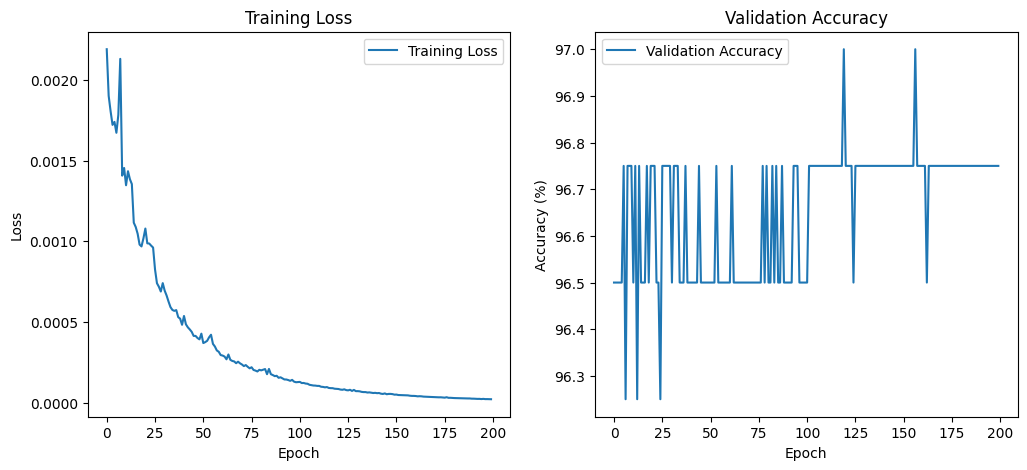
\includegraphics{cnu_deeplearning_files/figure-pdf/cell-17-output-2.png}



\end{document}
